\clearpage
\documentclass[a4paper,12pt,notitlepage]{article}

\frenchspacing
\usepackage{a4}
\usepackage[pdftitle={Vypracovane otazky k bakalarskym statnicim}, pdfauthor={študenti MFF}, pdfdisplaydoctitle=true, colorlinks=false,unicode=true,pdfborder=0 0 0]{hyperref}
\usepackage{slovak}
\usepackage{ucs}
\usepackage[utf8x]{inputenc}

\title{Vypracovane otazky k bakalarskym statnicim}
\author{študenti MFF}

\usepackage{graphicx}
\usepackage{amsmath,amssymb,amsthm}
\usepackage{color}
\usepackage[left=3cm, right=3cm, top=3cm, bottom=3cm]{geometry} % nastavení dané velikosti okrajů


%Vacsina prostredi je dvojjazicne. V pripade, ze znenie napr pozorovania je pisane po slovensky, malo by byt po slovensky aj oznacenie.

\newenvironment{pozadavky}{\pagebreak[2]\noindent\textbf{Požadavky}\par\noindent\leftskip 10pt}{\par\bigskip}
\newenvironment{poziadavky}{\pagebreak[2]\noindent\textbf{Požiadavky}\par\noindent\leftskip 10pt}{\par\bigskip}

\newenvironment{definice}{\pagebreak[2]\noindent\textbf{Definice}\par\noindent\leftskip 10pt}{\par\bigskip}
\newenvironment{definiceN}[1]{\pagebreak[2]\noindent\textbf{Definice~}\emph{(#1)}\par\noindent\leftskip 10pt}{\par\bigskip}
\newenvironment{definicia}{\pagebreak[2]\noindent\textbf{Definícia}\par \noindent\leftskip 10pt}{\par\bigskip}
\newenvironment{definiciaN}[1]{\pagebreak[2]\noindent\textbf{Definícia~}\emph{(#1)}\par\noindent\leftskip 10pt}{\par\bigskip}

\newenvironment{pozorovani}{\pagebreak[2]\noindent\textbf{Pozorování}\par\noindent\leftskip 10pt}{\par\bigskip}
\newenvironment{pozorovanie}{\pagebreak[2]\noindent\textbf{Pozorovanie}\par\noindent\leftskip 10pt}{\par\bigskip}
\newenvironment{poznamka}{\pagebreak[2]\noindent\textbf{Poznámka}\par\noindent\leftskip 10pt}{\par\bigskip}
\newenvironment{poznamkaN}[1]{\pagebreak[2]\noindent\textbf{Poznámka~}\emph{(#1)}\par\noindent\leftskip 10pt}{\par\bigskip}
\newenvironment{lemma}{\pagebreak[2]\noindent\textbf{Lemma}\par\noindent\leftskip 10pt}{\par\bigskip}
\newenvironment{lemmaN}[1]{\pagebreak[2]\noindent\textbf{Lemma~}\emph{(#1)}\par\noindent\leftskip 10pt}{\par\bigskip}
\newenvironment{veta}{\pagebreak[2]\noindent\textbf{Věta}\par\noindent\leftskip 10pt}{\par\bigskip}
\newenvironment{vetaN}[1]{\pagebreak[2]\noindent\textbf{Věta~}\emph{(#1)}\par\noindent\leftskip 10pt}{\par\bigskip}
\newenvironment{vetaSK}{\pagebreak[2]\noindent\textbf{Veta}\par\noindent\leftskip 10pt}{\par\bigskip}
\newenvironment{vetaSKN}[1]{\pagebreak[2]\noindent\textbf{Veta~}\emph{(#1)}\par\noindent\leftskip 10pt}{\par\bigskip}

\newenvironment{dusledek}{\pagebreak[2]\noindent\textbf{Důsledek}\par\noindent\leftskip 10pt}{\par\bigskip}
\newenvironment{dosledok}{\pagebreak[2]\noindent\textbf{Dôsledok}\par\noindent\leftskip 10pt}{\par\bigskip}

\newenvironment{dokaz}{\pagebreak[2]\noindent\leftskip 10pt\textbf{Dôkaz}\par\noindent\leftskip 10pt}{\par\bigskip}
\newenvironment{dukaz}{\pagebreak[2]\noindent\leftskip 10pt\textbf{Důkaz}\par\noindent\leftskip 10pt}{\par\bigskip}

\newenvironment{priklad}{\pagebreak[2]\noindent\textbf{Příklad}\par\noindent\leftskip 10pt}{\par\bigskip}
\newenvironment{prikladSK}{\pagebreak[2]\noindent\textbf{Príklad}\par\noindent\leftskip 10pt}{\par\bigskip}
\newenvironment{priklady}{\pagebreak[2]\noindent\textbf{Příklady}\par\noindent\leftskip 10pt}{\par\bigskip}
\newenvironment{prikladySK}{\pagebreak[2]\noindent\textbf{Príklady}\par\noindent\leftskip 10pt}{\par\bigskip}

\newenvironment{algoritmusN}[1]{\pagebreak[2]\noindent\textbf{Algoritmus~}\emph{(#1)}\par\noindent\leftskip 10pt}{\par\bigskip}
%obecne prostredie, ktore ma vyuzitie pri specialnych odstavcoch ako (uloha, algoritmus...) aby nevzniklo dalsich x prostredi
\newenvironment{obecne}[1]{\pagebreak[2]\noindent\textbf{#1}\par\noindent\leftskip 10pt}{\par\bigskip}


\newenvironment{penumerate}{
\begin{enumerate}
  \setlength{\itemsep}{1pt}
  \setlength{\parskip}{0pt}
  \setlength{\parsep}{0pt}
  %\setlength{\topsep}{200pt}
  \setlength{\partopsep}{200pt}
}{\end{enumerate}}

\def\pismenka{\numberedlistdepth=2} %pouzit, ked clovek chce opismenkovany zoznam...

\newenvironment{pitemize}{
\begin{itemize}
  \setlength{\itemsep}{1pt}
  \setlength{\parskip}{0pt}
  \setlength{\parsep}{0pt}
}{\end{itemize}}

\definecolor{gris}{gray}{0.95}
\newcommand{\ramcek}[2]{\begin{center}\fcolorbox{white}{gris}{\parbox{#1}{#2}}\end{center}\par}

\clearpage

\title{\LARGE Učební texty k státní bakalářské zkoušce \\ Matematika}


\begin{document}

\maketitle

\vspace{10mm}
\begin{center}

\includegraphics[scale=0.5]{../common/logo.pdf}
\end{center} 

\clearpage
\emph{Vážený studente/čtenáři},

po úspěšné edici vypracovaných otázek k bakalářským státnicím přichází očekávaný druhý díl, snažící se poskytnout studijní materiály i pro státní závěrečnou zkoušku na navazujícím magiterském programu.

Tento úkol je však řádově náročnější, než u bakalářských státnic, protože magisterské studium se dělí na více studijních oborů a ty dále na mnoho dalších studijních plánů.

Otázky jsou vypracované studenty, nebyly zkontrolované vyučujícími a není tedy garantovaná správnost ani úplnost i když se o ni snažíme.   

Velmi uvítáme, pokud do publikace přispějete. Mějte prosím na paměti, že publikace by měla být pokud možno psána česky a slovensky.

Texty je možné dále používat a šířit pod licencí \textbf{GNU GFDL}, což zároveň pro přispivatele znamená, že s uveřejněním svých textů pod touto licencí musí souhlasit. 

Věříme, že Vám tyto texty pomůžou s úspěšným složením státních zkoušek.

\begin{center}
\line(1,0){300}
\end{center}

\clearpage

\tableofcontents


\newpage
\section{Čísla}

\begin{pozadavky}
\begin{pitemize}
\item Vlastnosti přirozených, celých, racionálních, reálných a komplexních čísel
\item Posloupnosti a limity
\item Cauchyovské posloupnosti
\end{pitemize}
\end{pozadavky}

\subsection{Reálná čísla}
Množinou všech reálných čísel (značíme ji $\mathbb{R}$) budeme rozumět množinu, na níž je definováno sčítání (značíme $x+y$), násobení (značíme $x\cdot y$) a uspořádání (značíme $x \le y$), která spňují tyto axiomy:

\begin{penumerate}
	\item (Algebraické operace)
	\begin{penumerate}
		\item $\forall x,y,z \in \mathbb{R} : x+(y+z) = (x+y)+z \hfill\textit{(asociativní zákon pro sčítání)}$
		\item $\forall x,y \in \mathbb{R} : x+y = y+x \hfill\textit{(komutativní zákon pro sčítání)}$
		\item v $\mathbb{R}$ existuje nulový prvek (značíme ho 0) tak, že $\forall x \in \mathbb{R}: x+0 = x$
		\item pro každý $x \in \mathbb{R}$ existuje opačný prvek (značíme ho $-x$) tak, že $x+(-x)=0$
		\item $\forall x,y,z \in \mathbb{R}: x\cdot (y\cdot z)=(x\cdot y)\cdot z \hfill\textit{(asociativní zákon pro násobení)}$
		\item $\forall x,y \in \mathbb{R} : x\cdot y = y\cdot x \hfill\textit{(komutativní zákon pro násobení)}$
		\item v $\mathbb{R}$ existuje jednotkový prvek (značíme ho 1) tak, že $\forall x \in \mathbb{R}: x\cdot 1=x$
		\item pro každý $x \in \mathbb{R}, x \neq 0$ existuje inverzní prvek (značíme ho $x^{-1}$) tak, že $x\cdot x^{-1}=1$
		\item $\forall x,y,z \in \mathbb{R}: (x+y)\cdot z = x\cdot z + y\cdot z \hfill\textit{(distributivní zákon)}$
	\end{penumerate}
	\item (Uspořádání)
	\begin{penumerate}
		\item $\forall x,y,z \in \mathbb{R}: ((x \le y) \wedge (y \le z)) \Rightarrow (x \le z) \hfill\textit{(tranzitivita)}$
		\item $\forall x,y \in \mathbb{R}: (((x \le y) \wedge (y \le x)) \Rightarrow (x=y) \hfill\textit{(slabá antisymetrie)}$
		\item $\forall x,y \in \mathbb{R}: (x \le y) \vee (y \le x)$
		\item $\forall x,y,z \in \mathbb{R}: (x \le y) \Rightarrow (x+z \le y+z)$
		\item $\forall x,y,z \in \mathbb{R}: (x \le y) \wedge (0 \le z) \Rightarrow (x\cdot z \le y\cdot z)$
	\end{penumerate}
	\item (Netrivialita)
	\begin{penumerate}
		\item $0 \neq 1$
	\end{penumerate}
	\item (Úplnost)
		\\\begin{definiceN}{Axiom suprema}
		Nechť $M \subset \mathbb{R}$ je neprázdná a shora omezená. Pak existuje číslo $s \in \mathbb{R}$, které má vlastnosti:
		\begin{penumerate}
			\item $\forall x \in M: x \le s$
			\item $\forall s' \in \mathbb{R}, s' < s\;\; \exists x \in M: x > s'$
		\end{penumerate}
		
		Číslo $s$ z axiomu suprema je jednoznačně určeno, značí se $\sup M$ a říká se mu \emph{supremum množiny $M$}. Supremum množiny je její nejmenší horní závora (\emph{horní závora} je každý takový prvek, pro který platí bod (a) definice suprema). Největší dolní závoru množiny $M$ (pokud existuje -- a dá se dokázat, že existuje, je-li množina zdola omezená) nazýváme \emph{infimem množiny $M$} a značíme $\inf M$.
		\end{definiceN}
\end{penumerate}

\begin{poznamka}
Relace \uv{$<$} na reálných číslech (a stejně tak na přirozených a racionálních číslech) se definuje takto: $a<b$, právě když $a\leq b$ a zároveň $a\neq b$.
\end{poznamka}

\subsection{Přirozená čísla}

\begin{definice}
	Řekneme, že množina $S \subset \mathbb{R}$ je \emph{induktivní}, jestliže platí
	\begin{pitemize}
		\item $1 \in S$
		\item $[x \in S \Rightarrow (x+1) \in S]$
	\end{pitemize}
	Množinu \emph{přirozených čísel $\mathbb{N}$} definujeme jako průnik všech induktivních podmnožin $\mathbb{R}$, tedy
	$$
		N := \bigcap \{ S; S \subset \mathbb{R}; \textit{S induktivní}\}
	$$
\end{definice}

\begin{vetaN}{Induktivnost přirozených čísel}
	Množina $\mathbb{N}$ je induktivní.
\end{vetaN}

\begin{vetaN}{Vlastnosti přirozených čísel}
	Množina $\mathbb{N}$ má nasledujúcí vlastnosti:
	\begin{penumerate}
		\item $n \in \mathbb{N} \Rightarrow n \ge 1$
		\item $n \in \mathbb{N} \backslash \{1\} \Rightarrow \exists m \in \mathbb{N}: n=m+1$
		\item $m,n \in \mathbb{N}, m < n \Rightarrow m + 1 \le n$ %před pravou stranou \exists byt nemusi -- Tuetschek
		\item každá neprázdná podmnožina $\mathbb{N}$ má nejmenší prvek
	\end{penumerate}
\end{vetaN}

\begin{vetaN}{Archimédova vlastnost reálných čísel}
	Pro každé $x \in \mathbb{R}$ existuje $n \in \mathbb{N}$ takové, že $x < n$
\end{vetaN}

\begin{vetaN}{Peanove axiómy pre zavedenie prirodzených čísel}
\begin{pitemize}
	\item Existuje číslo 0 (to neznamená, že nula je prirodzené číslo, v $\mathbb{N}$ roli tejto nuly hraje jednotka).
	\item Na množine prirodzených čísel je definovaná unárna operácia \uv{nasledovník}, označovaná S.
	\item Neexistuje žiadne prirodzené číslo, ktorého nasledovníkom je 0.
	\item Rôzne prirodzené čísla majú rôznych nasledovníkov: $a \neq b \Rightarrow S(a) \neq S(b)$ (t.j. funkcia nasledovníka je prostá).
	\item Ak číslo 0 spĺňa nejakú vlastnosť a súčasne ju spĺňa každý nasledovník prirodzeného čísla, potom túto vlastnosť spĺňajú všetky prirodzené čísla (\emph{axióm matematickej indukcie}).
\end{pitemize}
\end{vetaN}

\begin{vetaN}{Konštrukcia prirodzených čísel založená na teórii množín}
	Označme $0 := \{ \}$ a definujme $S(a) = a \cup \{a\}$ pre všetky a. Množina prirodzených čísel je potom definovaná ako prienik všetkých množín obsahujúcich $0$, ktoré sú uzavreté vzhľadom na funkciu nasledovníka. Predpokladajúc platnost axiómu nekonečnosti, dá sa dokázať, že táto definícia spĺňa Peanove axiómy. \emph{Axióm nekonečnosti} vyzerá takto:
$$\exists\mathbb{N}:\emptyset\in\mathbb{N}\wedge(\forall x:x\in \mathbb{N}\Rightarrow x\cup\{x\}\in\mathbb{N})$$
	
	V \uv{klasickom} zápise čísel potom každému prirodzenému číslu zodpovedá množina prirodzených čísel menších ako ono samo, takže
	\begin{pitemize}
		\item $0=\{\}$
		\item $1 = \{0\} = \{\{ \}\}$
		\item $2 = \{0,1\} = \{0, \{0\}\} = \{\{ \}, \{\{ \}\}\}$
		\item $3 = \{0,1,2\} = \{0, \{0\}, \{0, \{0\}\}\} = \{\{ \}, \{\{ \}\}, \{\{ \}, \{\{ \}\}\}\}$
	\end{pitemize}

	$\mathbb{N}$ je uzavretá na sčítanie.
\end{vetaN}

\subsection{Celá a racionální čísla}
\begin{definice}
	Kromě symbolů $\mathbb{R}$ a $\mathbb{N}$, které jsme již zavedli, budeme značit symbolem $\mathbb{Z}$ množinu \emph{celých čísel}, tedy
	$$\mathbb{Z} = \mathbb{N} \cup \{0\} \cup \{-n, n \in \mathbb{N}\}$$
	a symbolem $\mathbb{Q}$ množinu \emph{racionálních čísel}, tedy
	$$\mathbb{Q} = \left\{ \frac{p}{q}, p \in \mathbb{Z}, q \in \mathbb{N} \right\}$$
	
	$\mathbb{Z}$ je uzavřena na sčítání, odčítání a násobení,
	$\mathbb{Q}$ je uzavřena na sčítání, odčítání, násobení a dělení nenulovým číslem.
	
\end{definice}

\begin{vetaN}{Existence celé části}
	Pro každé $x \in \mathbb{R}$ existuje právě jedno číslo $[x] \in \mathbb{Z}$ splňující
	$$x-1 < [x] \le x$$
	Toto číslo nazýváme \emph{celou částí čísla x}.
\end{vetaN}

\begin{vetaN}{Hustota $\mathbb{Q}$ a $\mathbb{R} \backslash \mathbb{Q}$}
	Nechť $a,b \in \mathbb{R}, a < b$. Pak existují $q \in \mathbb{Q}$ a $r \in \mathbb{R} \backslash \mathbb{Q}$ takové, že
	$$a < q < b,\ a < r < b$$
\end{vetaN}

\begin{vetaN}{o existenci n-té odmocniny}
	Nechť $x \in \mathbb{R}, x \ge 0$ a nechť $n \in \mathbb{N}$. Pak existuje právě jedno $y \in \mathbb{R}, y \ge 0$ takové, že $y^n = x$
\end{vetaN}

\subsection{Komplexní čísla}
\begin{definice}
Komplexním číslem nazveme číslo tvaru $a + bi$, kde $a,b \in \mathbb{R}$ nazýváme \textbf{reálnou a imaginární částí} komplexního čísla. Tento tvar komplexního čísla se nazývá \textbf{algebraický}. Písmeno $i$ značí \textbf{imaginární jednotku}, která se formálně zavádí jako číslo splňující rovnici $i^2 +1 = 0$ tj. jako $\sqrt{-1}$ , která v reálných číslech neexistuje.

Pokud je $b = 0$, je dotyčné číslo reálným číslem, tj. reálná čísla tvoří podmnožinu čísel komplexních. Pokud je $a = 0$, mluvíme o \textbf{ryze imaginárním čísle}.
\end{definice}

\subsubsection{Aritmetika}
$$(a + ib) + (c+ id) = (a+c) + i(b+d)$$
$$(a + ib) - (c+ id) = (a-c) + i(b-d)$$
$$(a + ib) \cdot (c+ id) = (ac-bd) + i(ad+bc)$$
$$\frac{a+ib}{c+id}  = \frac{(a+ib)(c-id)}{(c+id)(c-id)} = \frac{(ac+bd) + i(bc-ad)}{c^2+d^2} = \left( \frac{ac+bd}{c^2+d^2} \right) + i \left( \frac{bc-ad}{c^2+d^2} \right)$$

Komplexní čísla se zobrazují v \textbf{komplexní (Gaussově) rovině} jako body se souřadnicemi $[x,y]$; $x$ je reálná část komplexního čísla, $y$ imaginární část. Na ose $x$ leží reálná čísla, na ose $y$ ryze imaginární čísla.

Pojmem \textbf{komplexně sdružené číslo} komplexního čísla $z = a + ib$ se nazývá číslo $\bar{z} = a - ib$

\textbf{Absolutní hodnotu} komplexního čísla $z = a + bi$ lze vyjádřit takto:
$$|z| = \sqrt{a^2 + b^2}$$


Následující vlastnosti platí pro všechna komplexní čísla $z$ a $w$, není-li uvedeno jinak.

$$\overline{z + w} = \overline{z} + \overline{w}$$

$$\overline{zw} = \overline{z}\ \overline{w}$$

$$\overline{\left({\frac{z}{w}}\right)} = \frac{\overline{z}}{\overline{w}}, \textit{pro w nenulové}$$

$$\overline{z} = z, \textit{právě když je z reálné číslo}$$

$$\left| \overline{z} \right| = \left| z \right|$$

$${\left| z \right|}^2 = z\overline{z}$$

$$z^{-1} = \frac{\overline{z}}{{\left| z \right|}^2}, \textit{pro z nenulové}$$

\begin{figure}
\centering%
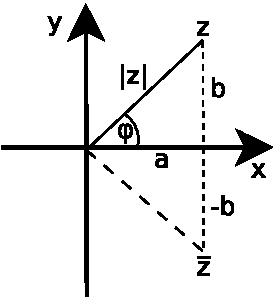
\includegraphics{matematika/obrazky/01-dia1}
\caption{Komplexní číslo ve 2D}
\label{fig:ComplexNum2D}
\end{figure}


Každé komplexní číslo z různé od nuly je možné jednoznačně vyjádřit v \textbf{goniometrickém tvaru}. Pokud si v komplexní rovině zvolíme polární souřadnicový systém, vzdálenost čísla $z$ od počátku je právě jeho absolutní hodnota $|z|$ (také nazývaná \textbf{modul}) a orientovaný úhel $\varphi = |\sphericalangle JOZ|$ (\emph{argument}), kde $J$ je bod $J[1,0]$, $O$ je počátkem soustavy a $Z$ je obraz komplexního čísla $a + bi$ se souřadnicemi $Z[a,b]$, platí:
$$z = |z| (\cos \varphi + i\cdot \sin \varphi)$$

Argument $\varphi$ lze vyjádřit ze vztahů: $\cos \varphi = \frac{a}{|z|}$ a $\sin \varphi = \frac{b}{|z|}$

Pro dělení komplexních čísel $z_1 = |z_1|\cdot (\cos\varphi_1 + i\cdot \sin
\varphi_1)$ a $z_2 = |z_2|\cdot (\cos \varphi_2 + i\cdot \sin \varphi_2)$ platí následující rovnice:
$$\frac{z_1}{z_2} = \frac{|z_1|}{|z_2|}\cdot \left[ \cos(\varphi_1 - \varphi_2) + i\cdot \sin(\varphi_1 - \varphi_2) \right]$$

Pro násobení komplexních čísel $z_1$ a $z_2$ z předchozího příkladu slouží vzorec:
$$z_1 \cdot  z_2 = |z_1|\cdot |z_2|\cdot \left[ \cos(\varphi_1 + \varphi_2) + i\cdot \sin(\varphi_1 + \varphi_2) \right]$$

Pro \textbf{n-tou mocninu komplexní čísla} v goniometrickém tvaru platí tzv. \textbf{Moivreova věta}:
$$z^n = |z|^n (\cos n \varphi + i\cdot \sin n \varphi)$$

\subsection{Posloupnosti a limity}
\begin{definiceN}{posloupnost}
\emph{Posloupností reálných čísel} nazýváme jakékoli zobrazení z množiny $\mathbb{N}$ do množiny $\mathbb{R}$. Posloupnost obvykle značíme symbolem $\{a_n\}^{\infty}_{n=1}$ nebo $\{a_n\}_{n \in \mathbb{N}}$. Pro každé konkrétní $n \in \mathbb{N}$ nazýváme reálné číslo $a_n$ \emph{n-tým členem} posloupnosti $\{a_n\}$.
\end{definiceN}

\begin{definiceN}{Omezené posloupnosti}
\begin{penumerate}
	\item Posloupnost $\{a_n\}$ je \emph{shora omezená}, je-li $\{a_n; n \in \mathbb{N}\}$ shora omezená.
	\item Posloupnost $\{a_n\}$ je \emph{zdola omezená}, je-li $\{a_n; n \in \mathbb{N}\}$ zdola omezená.
	\item Posloupnost $\{a_n\}$ je \emph{omezená}, je-li zdola omezená a shora omezená.
\end{penumerate}
\end{definiceN}

\begin{definiceN}{Rostoucí a klesající posloupnosti}
\begin{penumerate}
	\item Posloupnost $\{a_n\}$ je \emph{klesající}, jestliže $\forall n \in \mathbb{N}: a_n > a_{n+1}$.
	\item Posloupnost $\{a_n\}$ je \emph{rostoucí}, jestliže $\forall n \in \mathbb{N}: a_n < a_{n+1}$.
	\item Posloupnost $\{a_n\}$ je \emph{neklesající}, jestliže $\forall n \in \mathbb{N}: a_n \le a_{n+1}$.
	\item Posloupnost $\{a_n\}$ je \emph{nerostoucí}, jestliže $\forall n \in \mathbb{N}: a_n \ge a_{n+1}$.
	\item Posloupnost $\{a_n\}$ je \emph{monotónní}, jestliže je nerostoucí nebo neklesající.
	\item Posloupnost $\{a_n\}$ je \emph{ryze monotónní}, jestliže je rostoucí nebo klesající.
\end{penumerate}
\end{definiceN}

\subsubsection{Vlastní limity}
\begin{definice}
Nechť $\{a_n\}$ je posloupnost reálných čísel a $A \in \mathbb{R}$. Řekneme, že A je \emph{vlastní limitou posloupnosti} $\{a_n\}$, jestliže
$$\forall \varepsilon > 0\ \exists n_0 \in \mathbb{N}: \forall n \ge n_0, n \in \mathbb{N}: |a_n - A| < \varepsilon$$
značíme
$$\lim_{n \rightarrow \infty} a_n = A$$
\noindent Dá se jednoduše ukázat, že toto je splněno i pokud máme vždy od $n_0$ dále zaručeno jen to, že $|a_n - A| < K\cdot\varepsilon$ pro nějaké $K>0$.
\end{definice}

\begin{definice}
Jestliže existuje $A \in \mathbb{R}$ tak, že $\lim_{n \rightarrow \infty}a_n = A$, pak říkáme, že posloupnost $\{a_n\}$ má \emph{vlastní limitu} nebo že \emph{konverguje} (je \emph{konvergentní}). V opačném případě říkáme, že posloupnost \emph{diverguje}.
\end{definice}

\begin{pozorovani}
Ne každá posloupnost je konvergentní. Například posloupnost 0,1,0,1,0,... nemá vlastní limitu a podobně posloupnost $\{2^n\}$ nemá vlastní limitu.
\end{pozorovani}

\begin{priklady}
\begin{pitemize}
	\item $\lim_{n \rightarrow \infty} (\sqrt{n+1} - \sqrt{n}) = 0$
	\item $\lim_{n \rightarrow \infty} \sqrt[n]{n} = 1$
\end{pitemize}
\end{priklady}

\begin{vetaN}{o jednoznačnosti limity posloupnosti}
Každá posloupnost má nejvýše jednu limitu.
\end{vetaN}

\begin{vetaN}{o omezenosti konvergentní posloupnosti}
Každá konvergentní posloupnost je omezená.
\end{vetaN}

\begin{definice}
Nechť $\{a_n\}_{n \in \mathbb{N}}$ je posloupnost reálných čísel. Řekneme, že posloupnost $\{b_k\}_{k \in \mathbb{N}}$ je \emph{vybraná} z posloupnosti, neboli že posloupnost $\{b_k\}_{k \in \mathbb{N}}$ je \emph{podposloupností} posloupnosti $\{a_n\}_{n \in \mathbb{N}}$, jestliže existuje rostoucí posloupnost přirozených čísel $\{n_k\}$ taková, že $b_k = a_{n_k}$ pro všechna $k \in \mathbb{N}$.
\end{definice}

\begin{vetaN}{o limitě vybrané posloupnosti}
Nechť $\{a_n\}_{n \in \mathbb{N}}$ je posloupnost reálných čísel a nechť $\lim_{n \rightarrow \infty} a_n = A$. Nechť posloupnost $\{b_k\}_{k \in \mathbb{N}}$ je vybraná z posloupnosti $\{a_n\}_{n \in \mathbb{N}}$. Pak $\lim_{k \rightarrow \infty} b_k = A$.
\end{vetaN}

\begin{vetaN}{o aritmetice limit}
Nechť $\{a_n\}_{n \in \mathbb{N}}$ a $\{b_n\}_{n \in \mathbb{N}}$ jsou dvě posloupnosti reálných čísel a nechť $\lim_{n \rightarrow \infty} a_n = A \in \mathbb{R}$ a $\lim_{n \rightarrow \infty} b_n = B \in \mathbb{R}$. Pak platí:
\begin{penumerate}
	\item $\lim_{n \rightarrow \infty} (a_n+b_n) = A+B$
	\item $\lim_{n \rightarrow \infty} (a_n \cdot  b_n) = A\cdot B$
	\item je-li $\forall n \in \mathbb{N}: b_n \neq 0$ a $B \neq 0$, pak $\lim_{n \rightarrow \infty} \frac{a_n}{b_n}=\frac{A}{B}$
\end{penumerate}
\end{vetaN}

\begin{vetaN}{o limitě a uspořádání}
Nechť $\{a_n\}_{n \in \mathbb{N}}$ a $\{b_n\}_{n \in \mathbb{N}}$ jsou dvě posloupnosti reálných čísel a nechť $\lim_{n \rightarrow \infty} a_n = A \in \mathbb{R}$ a $\lim_{n \rightarrow \infty} b_n = B \in \mathbb{R}$. Pak platí:
\begin{penumerate}
	\item Jestliže $A < B$, potom $\exists n_0 \in \mathbb{N}\ \forall n > n_0: a_n < b_n$
	\item Jestliže $\exists n_0 \in \mathbb{N}\ \forall n \ge n_0: a_n \ge b_n$, pak $A \ge B$
\end{penumerate}

\noindent Pozor, ostrost nerovností v tomto případě je důležitá.
\end{vetaN}

\begin{vetaN}{o policajtech}
Nechť $\{a_n\}_{n \in \mathbb{N}}$, $\{b_n\}_{n \in \mathbb{N}}$ a $\{c_n\}_{n \in \mathbb{N}}$ jsou posloupnosti reálných čísel, splňující
\begin{penumerate}
	\item $\exists n_0 \in \mathbb{N}\ \forall n > n_0: a_n \le c_n \le b_n$
	\item $\lim_{n \rightarrow \infty}a_n = \lim b_n = A \in \mathbb{R}$
\end{penumerate}
Pak
$$
\lim c_n = A
$$
\end{vetaN}

\begin{vetaN}{o limitě součinu mizející ($\lim=0$) a omezené posloupnosti}
Nechť $\{a_n\}_{n \in \mathbb{N}}$ a $\{b_n\}_{n \in \mathbb{N}}$ jsou posloupnosti reálných čísel, nechť je $\lim_{n \rightarrow \infty} a_n = 0$ a $\{b_n\}$ omezená. Pak
$$
\lim_{n \rightarrow \infty}(a_n \cdot b_n) = 0
$$
\end{vetaN}

\subsubsection{Nevlastní limity}
\begin{definice}
Řekneme, že posloupnost  $\{a_n\}$ má \emph{nevlastní limitu} $+ \infty$, jestliže:
$$ \forall K \in \mathbb{R}\ \exists n_0 \in \mathbb{N}: \forall n \ge n_0, n \in \mathbb{N}: a_n \ge K $$

Obdobně řekneme, že posloupnost  $\{a_n\}$ má \emph{nevlastní limitu} $- \infty$, jestliže:
$$ \forall K \in \mathbb{R}\ \exists n_0 \in \mathbb{N}: \forall n \ge n_0, n \in \mathbb{N}: a_n \le K $$

Má-li posloupnost nevlastní limitu, říkáme o ní, že diverguje, stejně jako v případě, že žádnou limitu nemá.
\end{definice}

\begin{poznamka}
Všechny možné situace jsou znázorněny na následujícím diagramu:

limita posloupnosti:
\begin{pitemize}
	\item neexistuje
	\item existuje
	\begin{pitemize}
		\item vlastní
		\item nevlastní
		\begin{pitemize}
			\item $- \infty$
			\item $+ \infty$
		\end{pitemize}
	\end{pitemize}
\end{pitemize}

\end{poznamka}

\begin{definice}
Množinu $\mathbb{R}^* := \mathbb{R} \cup \{ + \infty, - \infty \}$ nazýváme \emph{rozšířenou reálnou osou}.
\end{definice}

\begin{poznamka}
Věty o jednoznačnosti limity, o limitě vybrané posloupnosti, o limitě a uspořádání a o policajtech platí v nezměněné podobě, jestliže připustíme nevlastní limity. Věta o omezenosti konvergentní posloupnosti zrejmě neplatí - neboť je-li $\lim_{n \rightarrow \infty} a_n=\infty$ (nebo $- \infty$), pak posloupnost $\{a_n\}$ není omezená. Větu o aritmetice limit pro rozšírenou osu uvedeme zvlášť.
\end{poznamka}

\begin{vetaN}{o aritmetice limit pro nevlastní limity}
Nechť $\{a_n\}_{n \in \mathbb{N}}$ a $\{b_n\}_{n \in \mathbb{N}}$ jsou dvě posloupnosti reálných čísel a nechť $\lim_{n \rightarrow \infty} a_n = A \in \mathbb{R}^*$ a $\lim_{n \rightarrow \infty} b_n = B \in \mathbb{R}^*$. Pak platí:
\begin{penumerate}
	\item $\lim_{n \rightarrow \infty} (a_n+b_n) = A+B \textit{, pokud je výraz A+B definován}$
	\item $\lim_{n \rightarrow \infty} (a_n \cdot  b_n) = A\cdot B\textit{, pokud je výraz }A\cdot B\textit{ definován}$
	\item je-li $\forall n \in \mathbb{N}: b_n \neq 0$ a $B \neq 0$, pak $\lim_{n \rightarrow \infty} \frac{a_n}{b_n}=\frac{A}{B} \textit{, pokud je výraz } \frac{A}{B} \textit{ definován}$
\end{penumerate}
\end{vetaN}

\begin{definiceN}{Supremum a infimum na rozšířené reálné ose}
\begin{pitemize}
	\item Nechť množina $A \subset \mathbb{R}$ je shora neomezená. Pak klademe $\sup A := +\infty$
	\item Nechť množina $A \subset \mathbb{R}$ je zdola neomezená. Pak klademe $\inf A := -\infty$
	\item Nechť $A=\emptyset$. Pak klademe $\sup A := -\infty$ a $inf A := +\infty$
\end{pitemize}
\end{definiceN}

\begin{poznamka}
Prázdná množina je jediná množina, jejíž supremum je menší než její infimum.
\end{poznamka}

\begin{vetaN}{o limitě podílu kladné a mizející posloupnosti}
Nechť $\{a_n\}_{n \in \mathbb{N}}$ a $\{b_n\}_{n \in \mathbb{N}}$ jsou posloupnosti reálných čísel, nechť je $\lim_{n \rightarrow \infty} a_n = A \in \mathbb{R}^*, A>0$ a nechť $\lim_{n \rightarrow \infty}\{b_n\}=0$. Nechť
$$
	\exists n_0 \in \mathbb{N} \textit{ } \forall n \ge n_0, n \in \mathbb{N}: b_n>0
$$
Pak
$$
	\lim_{n \rightarrow \infty} \frac{a_n}{b_n} = + \infty
$$
\end{vetaN}

\subsubsection{Monotónní posloupnosti}
\begin{vetaN}{o limitě monotónní posloupnosti}
Každá monotónní posloupnost má limitu.
\end{vetaN}

\begin{poznamka}
Je-li posloupnost neklesající (nerostoucí) a navíc shora (zdola) omezená, pak má vlastní limitu.
Je-li posloupnost neklesající (nerostoucí) a navíc shora (zdola) neomezená, pak má limitu $+ \infty$ ($- \infty$).
\end{poznamka}

\begin{definiceN}{Limes superior a limes inferior}
Nechť $\{a_n\}_{n \in \mathbb{N}}$ je posloupnost reálných čísel. Je-li $\{a_n\}$ shora omezená, definujeme posloupnost $\{b_n\}_{n \in \mathbb{N}}$ předpisem:
$$
	b_n := \sup\{a_k; k \ge n \}
$$
Je-li $\{a_n\}$ zdola omezená, definujeme posloupnost $\{c_n\}_{n \in \mathbb{N}}$ předpisem:
$$
	c_n := \inf\{a_k; k \ge n \}
$$
V takovém případě definujeme:
$$
\lim \sup~a_n := \left\{
\begin{array}{ll} \lim_{n \rightarrow \infty} b_n & \textit{jestliže je } \{a_n\} \textit{ shora omezená} \\ \infty & \textit{jestliže je } \{a_n\} \textit{ shora neomezená} \end{array}
\right.
$$
Tuto hodnotu nazýváme \emph{limes superior} posloupnosti $\{a_n\}_{n \in \mathbb{N}}$. Obdobně definujeme \emph{limes inferior} posloupnosti $\{a_n\}_{n \in \mathbb{N}}$ předpisem:
$$
\lim \inf~a_n := \left\{
\begin{array}{ll} \lim_{n \rightarrow \infty} c_n & \textit{jestliže je } \{a_n\} \textit{ zdola omezená} \\ - \infty & \textit{jestliže je } \{a_n\} \textit{ zdola neomezená} \end{array}
\right.
$$
\end{definiceN}

\begin{poznamka}
Limes superior a limes inferior jsou vždy dobře definované hodnoty a platí
$$
\lim \sup~a_n \in \mathbb{R}^*, \lim \inf~a_n \in \mathbb{R}^*, 
$$
Na rozdíl od limity, která nemusí existovat, tyto dvě hodnoty existují pro
libovolnou posloupnost reálných čísel.
\end{poznamka}

\begin{vetaN}{o vztahu limity, limes superior a limes inferior}
Nechť $\{a_n\}_{n \in \mathbb{N}}$ je posloupnost reálných čísel. Potom 
$$
	\lim a_n = A \in \mathbb{R}^{*}
$$
právě tehdy, když
$$
\lim \sup~a_n = \lim \inf~a_n = A \in \mathbb{R}^*
$$
\end{vetaN}

\begin{definice}
Nechť $\{a_n\}_{n \in \mathbb{N}}$ je posloupnost reálných čísel. Pak $A \in \mathbb{R}^*$ nazveme \emph{hromadnou hodnotou} posloupnosti $\{a_n\}$, jestliže existuje vybraná posloupnost taková $\{a_{n_k}\}$, že $\lim_{k \rightarrow \infty} a_{n_k} = A$. Množina všech hromadných hodnot značíme $H(\{a_n\})$
\end{definice}

\begin{vetaN}{o vztahu limes superior, limes inferior a hromadných hodnot}
Nechť $\{a_n\}_{n \in \mathbb{N}}$ je posloupnost reálných čísel. Potom $H\{(a_n)\} \neq \emptyset$,
$$
\lim \sup~a_n = \max H(\{a_n\}) \textit{ a } \lim \inf~a_n = \min H(\{a_n\})
$$
\end{vetaN}

\subsection{Cauchyovské posloupnosti}

Tato sekce je vypracovaná podle skript Prof. A. Pultra z matematické analýzy\\
(\texttt{http://kam.mff.cuni.cz/\~{}pultr/})
\bigskip

\begin{definiceN}{Bolzano-Cauchyova podmínka}
Řekneme, že posloupnost $\{a_n\}_{n\geq 0}$ je \emph{cauchyovská}, nebo-li že splňuje \emph{Bolzano-Cauchyho podmínku}, pokud pro ní platí:
$$
\forall \varepsilon > 0~~\exists n_0 \in \mathbb{N}: \forall m, n \in \mathbb{N}: m \ge n_0, n \ge n_0: |a_n - a_m| < \varepsilon
$$
\end{definiceN}

\begin{vetaN}{Bolzano-Weierstrassova}
Z každé omezené posloupnosti lze vybrat konvergentní podposloupnost. Jsou-li $a_n$ v kompaktním intervalu $[a,b]$, je limita vybrané posloupnosti v tomto intervalu.

\medskip\begin{dukaz}
První část dokážeme nalezením takové posloupnosti. Vezmeme $A:=\lim\sup~a_n$ a definujeme pro každé $k\in\mathbb{N}$ množinu $M_k:=\{j\in\mathbb{N}|j>n_{k-1},a_j\in\langle A - \frac{1}{2^k}, A + \frac{1}{2^k}\rangle\}$ a $n_k:=\min M_k$. Potom $\{a_{n_k}\}$ je vybraná posloupnost, která konverguje. Druhá část je přímým důsledkem věty o limitě a uspořádání.
\end{dukaz}
\end{vetaN}

\begin{lemma}
Má-li cauchyovská posloupnost konvergentní podposloupnost, je konvergentní.

\medskip\begin{dukaz}
Nechť $\lim a_{n_k} = x$. Pro $\varepsilon > 0$ zvolme $n_0$, aby pro $m,n\geq n_0$ platilo $|a_m-a_n|<\frac{\varepsilon}{2}$ a $|a_k-x|<\frac{\varepsilon}{2}$. Protože $k_n\geq n$, platí $|a_n-x|=|a_n-a_{k_n}|+|a_{k_n}-x|<\varepsilon$.
\end{dukaz}
\end{lemma}


\begin{vetaN}{Bolzano-Cauchyova}
Posloupnost $\{a_n\}$ má vlastní limitu, právě když je cauchyovská.

\medskip\begin{dukaz}
\begin{penumerate}
    \item Implikace \uv{$\Rightarrow$} je hned vidět -- stačí vzít k $\varepsilon$ takové $n_0$, že $|a_n-x|<\frac{\varepsilon}{2}\ \forall n\geq n_0$. Potom je $|a_n-a_m|=|a_n-x+x-a_m|\leq|a_n-x|+|x-a_m|\leq\varepsilon\ \forall m,n\geq n_0$.\medskip
    \item Pro druhou implikaci stačí dokázat, že je cauchyovská posloupnost omezená a zbytek dostaneme z předchozího lemmatu a Bolzano-Weierstrassovy věty. Pro $\varepsilon=1$ existuje $n_0$ takové, že $a_{n_0}-1<a_n<a_{n_0}+1$ pro každé $n\geq n_0$ (to plyne přímo z podmínky), takže zbývá jen konečný počet členů mimo toto rozmezí (pro $n<n_0$), a ty vždy tvoří omezený systém.
\end{penumerate}
\end{dukaz}
\end{vetaN}


\newpage
\def\tg{\mathrm{tg}}
\def\cotg{\mathrm{cotg}}
\def\arctg{\mathrm{arctg}}
\def\arccotg{\mathrm{arccotg}}

\section{Základy diferenciálního počtu}

\begin{pozadavky}
\begin{pitemize}
	\item Reálné funkce jedné reálné proměnné
	\item Spojitost, limita funkce v bodě (vlastní i nevlastní)
	\item Některé konkrétní funkce (polynomy, racionální lomené funkce, goniometrické a cyklometrické funkce, logaritmy a exponenciální funkce)
	\item Derivace: definice a základní pravidla, věty o střední hodnotě, derivace vyšších řádů
	\item Některé aplikace (průběhy funkcí, Newtonova metoda hledání nulového bodu, Taylorův polynom se zbytkem)
\end{pitemize}
\end{pozadavky}

\subsection{Reálné funkce jedné reálné proměnné}
\begin{definiceN}{Reálná funkce}
Reálná funkce jedné proměnné je zobrazení $f: M \rightarrow \mathbb{R}$, kde $M \subseteq \mathbb{R}$. \\
$f$ je na $M$:
\begin{pitemize}
	\item \emph{rostoucí}: $\forall x, y: x < y \Rightarrow f(x) < f(y)$
	\item \emph{klesající}: $\forall x, y: x < y \Rightarrow f(x) > f(y)$
	\item \emph{neklesající}: $\forall x, y: x < y \Rightarrow f(x) \le f(y)$
	\item \emph{nerostoucí}: $\forall x, y: x < y \Rightarrow f(x) \ge f(y)$

	\item \emph{sudá}: $x \in M \Rightarrow -x \in M \wedge f(x)=f(-x), \forall x \in M$
	\item \emph{lichá}: $x \in M \Rightarrow -x \in M \wedge f(x)=-f(-x), \forall x \in M$
	\item \emph{periodická} s periodou $p\in\mathbb{R}$: $x \in M \Rightarrow x \pm p \in M \wedge f(x)=f(x+p)=f(x-p), \forall x \in M$
\end{pitemize}
\end{definiceN}

\begin{definiceN}{Okolí bodu}
$P(a, \delta) = (a-\delta, a) \cup (a, a+\delta)$ (prstencové okolí)

\noindent
$P^{+}(a, \delta)=(a, a+\delta)$ (pravé prstencové okolí)

\noindent
$P^{-}(a, \delta)=(a-\delta, a)$ (levé prstencové okolí)

\noindent
$B(a, \delta)=(a-\delta, a+\delta) = P(a, \delta)+\{a\}$ ($\delta$-okolí)

\noindent
Podobně se definuje i levé a pravé $\delta$-okolí bodu $a$.
\end{definiceN}

\subsection{Spojitost, limita funkce v bodě (vlastní i nevlastní)}

\begin{definiceN}{Limita}
Řekneme, že $f$ má v bodě $a \in \mathbb{R}^{*}$ limitu $A \in \mathbb{R^{*}}$, jestliže
$$\forall \varepsilon>0\ \exists \delta>0: \forall x \in P(a, \delta) \Rightarrow f(x) \in B(A, \varepsilon)$$
a značíme $\lim_{x \rightarrow a} f(x) = A$

\medskip
Platí-li tato vlastnost jen pro pravá okolí bodů $a$ a $A$, mluvíme o \emph{jednostranné limitě zprava} a podobně zleva.
\end{definiceN}

\begin{definiceN}{Spojitost v bodě}
Řekneme, že $f$ je spojitá v bodě $a \in \mathbb{R}$, jestliže $\lim_{x \rightarrow a} f(x) = f(a)$
\end{definiceN}

\begin{vetaN}{Heineho věta}
Nechť  $f: M \rightarrow \mathbb{R}, M \subseteq \mathbb{R}$. Nechť $f$ je definováno na nějakém prstencovém okolí bodu $a \in \mathbb{R}^{*}$. Potom následující dvě tvrzení jsou ekvivalentní:
\begin{penumerate}
	\item $lim_{x \rightarrow a} f(x) = A \in \mathbb{R}^{*}$
	\item Pro každou posloupnost $\{x_n\}_{n=1}^{\infty}$ splňující $x_n \in D(f)\ \forall n \in \mathbb{N}$ a  $\lim x_n = a, x_n \neq a\ \forall n$ platí $\lim_{n \rightarrow \infty} f(x_n)=A$
\end{penumerate}
Heineho věta umožňuje tvrzení, vyslovená o limitách posloupností, převádět na limity funkcí v bodě.
\end{vetaN}

\begin{vetaN}{Věta o jednoznačnosti limity funkce}
Funkce $f$ má v každém bodě nejvýše jednu limitu.
\end{vetaN}

\begin{vetaN}{O lokální omezenosti funkce s vlastní limitou}
Nechť funkce $f$ má v bodě $a \in \mathbb{R}^{*}$ vlastní limitu. Potom existuje $\delta > 0$ takové, že $f$ je na $P(a, \delta)$ omezená.
\end{vetaN}

\begin{vetaN}{Aritmetika limit pro funkce}
Nechť $\lim_{x \rightarrow a} f(x)=A$, $\lim_{x \rightarrow a} g(x)=B$, $a \in R^{*}$. Potom
\begin{penumerate}
	\item $\lim (f(x)+g(x)) = A+B$, je-li výraz na pravé straně definován.
	\item $\lim (f(x)g(x)) = A\cdot B$, je-li výraz na pravé straně definován.
	\item $\lim \frac{f(x)}{g(x)} = \frac{A}{B}$, je-li výraz na pravé straně definován.
\end{penumerate}
\end{vetaN}

\begin{vetaN}{Limita a uspořádání - policajti pro funkce}
\begin{penumerate}
	\item Nechť $\lim_{x \rightarrow a} f(x) > \lim_{x \rightarrow a} g(x)$, $a \in R^{*}$.\\Potom $\exists P(a, \delta): f(x)>g(x) \ \forall x \in P(a, \delta)$
	\item Nechť $f(x) \le g(x), \forall x \in P(a, \delta), \delta > 0$ a existují $\lim_{x \rightarrow a} f(x)$, $\lim_{x \rightarrow a} g(x)$.\\Potom $\lim_{x\to a} f(x) \le \lim_{x\to a} g(x)$.
	\item Nechť $f(x) \le h(x) \le g(x), \forall x \in P(a, \delta), \delta > 0$ a $\lim_{x \rightarrow a} f(x) = \lim_{x \rightarrow a} g(x)$.\\Potom existuje $\lim h(x)$ a $\lim_{x \rightarrow a} h(x) = \lim_{x \rightarrow a} f(x) = \lim_{x \rightarrow a} g(x)$.
\end{penumerate}
Pozor na ostrost nerovností, v tomto případě je velmi důležitá.
\end{vetaN}

\begin{definiceN}{Jednostranná spojitost funkce v bodě}
\begin{pitemize}
	\item $\textit{funkce f je spojitá v a} \Leftrightarrow \lim_{x \rightarrow a} f(x)=f(a) \Leftrightarrow \forall \varepsilon>0~\exists \delta >0: f(B(a, \delta)) \subseteq B(f(a), \varepsilon)$
	\item $\textit{funkce f je spojitá v a zprava} \Leftrightarrow \lim_{x \rightarrow a^{+}} f(x)=f(a) \Leftrightarrow \forall \varepsilon>0~\exists \delta >0: f(B^{+}(a, \delta)) \subseteq B(f(a), \varepsilon)$
	\item $\textit{funkce f je spojitá v a zleva} \Leftrightarrow \lim_{x \rightarrow a^{-}} f(x)=f(a) \Leftrightarrow \forall \varepsilon>0~\exists \delta >0: f(B^{-}(a, \delta)) \subseteq B(f(a), \varepsilon)$
\end{pitemize}
\end{definiceN}

\begin{vetaN}{O limitě složené funkce}
Nechť $\lim_{x \rightarrow a} g(x) = A$, $\lim_{y \rightarrow A} f(y) = B$, $a, A, B \in \mathbb{R}^{*}$. Nechť navíc platí jeden z předpokladů:\\
(P1) $f$ je spojitá v $A$\hfill \textit{(vnější funkce je spojitá)}\\
(P2) $\exists \delta > 0: g(x) \neq A$ pro $\forall x \in P(a, \delta)$\hfill \textit{(vnitřní je \uv{lokálně prostá})}\\
Potom $\lim_{x \rightarrow a} (f \circ g)(x) = B$.
\end{vetaN}

\begin{definiceN}{Interval}
Nechť $a, b \in \mathbb{R}^{*}, a < b$. Pak \emph{otevřeným intervalem} $(a, b)$ nazveme $\{x | a<x<b\}$, \emph{(uzavřeným) intervalem} $\left<a, b\right>$ (pro $a, b \in \mathbb{R}$) nazveme $I=\{x | a \le x \le b\}$. Uzavřený interval se někdy značí i $[a,b]$.
\end{definiceN}

\begin{vetaN}{Věta o limitě monotónní funkce}
Nechť je funkce $f$ monotónní na $(a, b)$, $a, b \in \mathbb{R}^{*}, a < b$. Potom $\exists \lim_{x \rightarrow a^{+}} f(x)$, $\exists \lim_{x \rightarrow b^{-}} f(x)$.
\end{vetaN}

\begin{definiceN}{Spojitost na intervalu}
Je-li $\left<a, b\right>$ interval, pak $a$ nazýváme počátečním bodem, $b$ koncovým bodem a $x \in (a, b)$ vnitřními body.

Řekneme, že $f$ \emph{je spojitá na intervalu $I$}, jestliže je spojitá zprava ve všech bodech kromě koncového a spojitá zleva ve všech bodech kromě počátečního.
\end{definiceN}

\begin{vetaN}{O spojitém obrazu intervalu}
Nechť funkce $f: I \rightarrow \mathbb{R}$ je spojitá na intervalu $I$. Potom $f(I)$ je také interval.
\end{vetaN}

\begin{vetaN}{Darbouxova o nabývaní mezihodnot}
Nechť funkce $f$ je spojitá na $\left<a, b\right>$ a $f(a)<f(b)$, potom $\forall y \in (f(a), f(b))$ existuje $x \in (a, b)$ takové, že $f(x)=y$.
\end{vetaN}

\begin{definice}
$f: M \rightarrow \mathbb{R}, M \subseteq \mathbb{R}$. $f$ nabývá v bodě $a \in M$:
\begin{pitemize}
	\item \emph{maxima} na M $\Leftrightarrow \forall x \in M: f(x) \le f(a)$
	\item \emph{minima} na M $\Leftrightarrow \forall x \in M: f(x) \ge f(a)$
	\item \emph{ostrého maxima} na M $\Leftrightarrow \forall x \in M\setminus \{a\}: f(x) < f(a)$
	\item \emph{ostrého minima} na M $\Leftrightarrow \forall x \in M\setminus \{a\}: f(x) > f(a)$
	\item \emph{lokálního} maxima (minima, ostrého...)$\Leftrightarrow \exists \delta > 0: f$ nabývá na $M \bigcap B(a, \delta)$ maxima (minima, ...)
\end{pitemize}
\end{definice}

\begin{vetaN}{Vztah spojitosti a extrémů}
Nechť $f$ je spojitá na $\left<a, b\right>$. Potom $f$ nabývá na $\left<a, b\right>$ svého maxima i minima.
\end{vetaN}

\begin{vetaN}{Vztah spojitosti a omezenosti}
Spojitá funkce na uzavřeném intervalu $\left<a, b\right>$ je omezená.
\end{vetaN}

\begin{definiceN}{prostá funkce, inverzní funkce}
Funkce $f$ je \emph{prostá}, jestliže $\forall x, y \in D(f): x \neq y \Rightarrow f(x) \neq f(y)$.

Nechť $f$ je prostá na $M$, tedy $f: M \rightarrow f(M)$. Pak \emph{inverzní funkce} $f^{-1}$ k funkci $f$ je definovaná na $f(M)$ předpisem: $y \in f(M)$, pak $f^{-1}(y)=x \Leftrightarrow y=f(x)$.
\end{definiceN}

\begin{vetaN}{O inverzní funkci}
Nechť $I$ je interval a funkce $f$ je definovaná, spojitá a rostoucí (klesající) na $I$. Potom inverzní funkce $f^{-1}$ je definována, spojitá a rostoucí (klesající) na $f(I)$.
\end{vetaN}

\subsection{Některé konkrétní funkce (polynomy, racionální lomené funkce, goniometrické a cyklometrické funkce, logaritmy a exponenciální funkce)}

\begin{vetaN}{Exponenciální funkce}
Existuje právě jedna reálná funkce \textbf{exp}, splňující:
\begin{pitemize}
	\item $\exp(x+z)=\exp(x) \exp(z), \forall x,z \in \mathbb{R}$
	\item $\exp(x) \ge 1+x, \forall x \in \mathbb{R}$
\end{pitemize}
\end{vetaN}

\begin{poznamkaN}{Některé vlastnosti $\exp$}
Platí:
\begin{pitemize}
    \item $\exp 0=1$
    \item $\exp (-x) = \frac{1}{\exp x}$
    \item $\exp (x) \neq 0\ \forall x\in \mathbb{R}$
    \item $\lim_{x\to\infty}\exp x=\infty$, $\lim_{x\to-\infty}\exp x=0$
    \item $\exp$ je rostoucí na $\mathbb{R}$
    \item $\lim_{x\to 0}\frac{\exp x - 1}{x}=1$
\end{pitemize}
\end{poznamkaN}

\begin{vetaN}{Vlastnosti $\log$}
Funkce $\log$, definovaná předpisem $\log=\exp^{-1}$ má následující vlastnosti:
\begin{pitemize}
	\item $D(\log)=(0, \infty)$, $\log ((0, \infty)) \rightarrow \mathbb{R}$
	\item $\log(x\cdot y) = \log x + \log y, \forall x, y \in (0, \infty)$, $\log(x^n)=n\log x$
	\item log je spojitá, rostoucí na $(0, \infty)$, $\log 1=0$, $\log e = 1$
	\item $lim_{x \rightarrow 0_{+}} \log x = - \infty$, $lim_{x \rightarrow \infty} \log x = \infty$
	\item $lim_{x \rightarrow 1} \frac{\log x}{x-1} = 1$, $lim_{x \rightarrow 0} \frac{\log x+1}{x} = 1$
\end{pitemize}
\end{vetaN}

\begin{definiceN}{obecná mocnina}
Obecná mocnina $a^b=\exp(b \log a)$ pro $a>0, b \in \mathbb{R}$. Speciálně pro $a=e: e^x=\exp x$
\end{definiceN}

\begin{veta}
Existuje právě jedna reálná funkce $s$ a právě jedna reálná funkce $c$ taková, že:

\begin{pitemize}
	\item $s(x+y) = s(x)c(y) + c(x)s(y)$
	\item $c(x+y) = c(x)c(y) - s(x)s(y)$
	\item $s$ je lichá, $c$ sudá
	\item $s>0~\textit{na}~(0,1), s(1)=0$
\end{pitemize}
\end{veta}

\begin{definice}
\noindent Podle $s$ a $c$ definujeme \emph{Goniometrické funkce}:\\
$\sin(x)=s(\frac{x}{\pi})$, $\cos(x)=c(\frac{x}{\pi})$, $\tg(x)=\frac{\sin(x)}{\cos(x)}$, $\cotg(x)=\frac{\cos(x)}{\sin(x)}$

\noindent \emph{Cyklometrické funkce}:
\begin{pitemize}
	\item $\arcsin x = y \Leftrightarrow y \in <-\frac{\pi}{2}, \frac{\pi}{2}> \wedge \sin y=x$
	\item $\arccos x = y \Leftrightarrow y \in <0, \pi> \wedge \cos y=x$
	\item $\arctg~x = y \Leftrightarrow y \in (-\frac{\pi}{2}, \frac{\pi}{2}) \wedge \tg~y=x$
	\item $\arccotg~x = y \Leftrightarrow y \in (0, \pi) \wedge \cotg~y=x$
\end{pitemize}

\noindent a platí
$$\lim_{x \rightarrow 0} \frac{\arcsin x}{x} = 1$$
$$\lim_{x \rightarrow 0} \frac{\arccos x}{\sqrt{1-x}} = \lim_{x \rightarrow 0} \frac{\arctg x}{x} = 1$$
\end{definice}

\subsection{Derivace: definice a základní pravidla, věty o střední hodnotě, derivace vyšších řádů}
\begin{definice}
Nechť $f$ je reálná funkce jedné proměnné, $a \in \mathbb{R}$. Derivací funkce $f$ v bodě $a$ nazveme
$$f'(a) = \lim_{h \rightarrow 0} \frac{f(a+h)-f(a)}{h} \textrm{, pokud existuje}$$

\noindent Derivací zprava a zleva rozumíme:
$$f'_{+}(a) = \lim_{h \rightarrow 0_+} \frac{f(a+h)-f(a)}{h}, \, f'_{-}(a) = \lim_{h \rightarrow 0_-} \frac{f(a+h)-f(a)}{h}$$
\end{definice}

\begin{vetaN}{Vztah derivace a spojitosti}
Má-li $f$ v $a$ vlastní derivaci, potom je $f$ v $a$ spojitá.
\end{vetaN}

\begin{vetaN}{Aritmetika derivací}
Nechť existují $f'(a)$, $g'(a)$:
\begin{penumerate}
	\item $(f+g)'(a)=f'(a)+g'(a)$, je-li pravá strana definována
	\item je-li $g$ nebo $f$ spojitá v $a$, pak $(fg)'(a)=f'(a)g(a)+f(a)g'(a)$
	\item je-li $g$ spojitá v $a$, $g(a) \neq 0$, pak $(\frac{f}{g})'(a)=\frac{f'(a)g(a)-f(a)g'(a)}{g^2(a)}$
\end{penumerate}
\end{vetaN}

\begin{vetaN}{O derivaci složené funkce}
Nechť funkce $f$ má derivaci v $y_0$, $g$ má derivaci v $x_0$, $g$ je spojitá v $x_0$ a $y_0=g(x_0)$. Potom $(f \circ g)'(x_0)=f'(y_0)\cdot g'(x_0)=f'(g(x_0))\cdot g'(x_0)$.
\end{vetaN}

\begin{vetaN}{O derivaci inverzní funkce}
Nechť funkce $f$ je na intervalu $(a,b)$ spojitá a ryze monotonní a má v bodě $x_0 \in (a,b)$ derivaci $f'(x_0)$ vlastní a různou od nuly. Potom má funkce $f^{-1}$ derivaci v bodě $y_0=f(x_0)$ a platí rovnost
$$(f^{-1})'(y_0) = \frac{1}{f'(f^{-1}(y_0))}.$$
\begin{poznamka}
Pokud v situaci popsané v právě uvedené větě je $f'(x_0)$ nevlastní, je $(f^{-1})'(y_0)=0$. Je-li $f'(x_0)=0$, je $(f^{-1})'(y_0)=+\infty$ (je-li $f$ rostoucí), resp. $=-\infty$ (je-li $f$ klesající).
\end{poznamka}
\end{vetaN}

\begin{vetaN}{Nutná podmínka lokálního extrému}
Nechť $M \subseteq \mathbb{R}$, $f: M \rightarrow \mathbb{R}$. Nechť $f$ má v $a \in M$ lokální extrém. Pak buď neexistuje $f'(a)$, nebo $f'(a)=0$.
\end{vetaN}

\begin{vetaN}{Rolleova věta}
Nechť $f$ je spojitá na $\left<a, b\right>$ a nechť existuje $f'(x)\ \forall x \in (a,b)$. Nechť $f(a)=f(b)$. Potom existuje $\xi \in (a,b): f'(\xi)=0$.
\end{vetaN}

\begin{vetaN}{Lagrangeova o střední hodnotě}
Nechť $f$ je spojitá na $\left<a, b\right>$ a nechť existuje $f'(x)\ \forall x \in (a,b)$. Potom existuje $$\xi \in (a,b): f'(\xi)=\frac{f(b)-f(a)}{b-a}$$
\end{vetaN}

\begin{vetaN}{Cauchyova o střední hodnotě}
Nechť $f$ a $g$ jsou spojité na $\left<a, b\right>$, nechť existuje $f'(x)\ \forall x \in (a,b)$ a nechť existuje $g'(x)$ vlastní a nenulové. Potom existuje $$\xi \in (a,b): \frac{f(b)-f(a)}{g(b)-g(a)}=\frac{f'(\xi)}{g'(\xi)}$$

\begin{dukaz}
$g(a) \neq g(b)$, neboť jinak by podle Rolleovy věty existovalo $\xi \in (a,b): g'(\xi)=0$. Definujeme $H(x)=(f(x)-f(a))(g(b)-g(a))-(g(x)-g(a))(f(b)-f(a))$. Potom $H(a)=H(b)=0$, $H$ je spojitá na $\left<a, b\right> \Rightarrow \exists H' na (a,b)$. Tedy podle Rolleovy věty $\exists \xi: 0 = H'(\xi)=f'(\xi)(g(b)-g(a))-g'(\xi)(f(b)-f(a))$. Tedy $\frac{f(b)-f(a)}{g(b)-g(a)}=\frac{f'(\xi)}{g'(\xi)}$, neboť $g'(\xi) \neq 0$ a $g(b)-g(a)\neq 0$ 
\begin{flushright}$\square$\end{flushright}
\end{dukaz}
\end{vetaN}

\begin{vetaN}{L'Hospitalovo pravidlo}
\csprimeson
Nechť $a \in \mathbb{R}^{*}$ a funkce $f$, $g$ jsou definovány na nějakém $P(a, \delta)$, $f, g$ mají v $P(a,\delta)$ vlastní derivaci, $\forall x \in P(a,\delta): g'(x)\not=0$ a existuje $\lim_{x \rightarrow a} \frac{f'(x)}{g'(x)}$. Nechť platí i jedna z následujících podmínek:
\begin{penumerate}
	\item $\lim_{x \rightarrow a} f(x)=\lim_{x \rightarrow a} g(x)=0$
	\item $\lim_{x \rightarrow a+} |g(x)|=+\infty$
\end{penumerate}
Potom existuje i $\lim_{x \rightarrow a} \frac{f(x)}{g(x)}$ a platí $\lim_{x \rightarrow a} \frac{f(x)}{g(x)}=\lim_{x \rightarrow a} \frac{f'(x)}{g'(x)}$.
\end{vetaN}

\begin{vetaN}{O limitě derivací}
Nechť funkce $f$ je spojitá zprava v $a \in \mathbb{R}$ a nechť existuje $\lim_{x \rightarrow a_+} f'(x)=A \in \mathbb{R}^*$. Potom $f'_+(a)=A$.
\end{vetaN}

\begin{vetaN}{Vztah derivace a monotonie}
Nechť $I$ je nezdegenerovaný interval (tj. nejde o jediný bod) a $Int(I)=\{\textit{vnitřní body I}\}$. Nechť $f$ je spojitá na $I$ a existuje $f'$ vlastní na $Int(I)$.:
\begin{penumerate}
	\item je-li $f' > 0$ na $Int(I)$, pak f je rostoucí na I
	\item je-li $f' \ge 0$ na $Int(I)$, pak f je neklesající na I
	\item je-li $f' < 0$ na $Int(I)$, pak f je klesající na I
	\item je-li $f' \le 0$ na $Int(I)$, pak f je nerostoucí na I
\end{penumerate}
\end{vetaN}

\begin{definiceN}{Tečna, inflexe}
Nechť funkce $f$ má v $a \in \mathbb{R}$ vlastní derivaci. Označíme $T_a=\{[x,y]\in \mathbb{R}^2, y=f(a)+f'(a)(x-a)\}$. Řekneme, že $[x, f(x)] \in \mathbb{R}^2$ leží nad (pod) tečnou $T_a$, jestliže $f(x)>f(a)+f'(a)(x-a)$ ($f(x)<f(a)+f'(a)(x-a)$).

Nechť $f$ má v $a \in \mathbb{R}$ vlastní derivaci. Řekneme, že $f$ má v $a$ \emph{inflexi}, jestliže $\exists \delta > 0$: buď $\forall x \in (a-\delta, a): [x, f(x)]$ leží nad $T_a$ $\wedge$ $\forall x \in (a, a+\delta): [x, f(x)]$ leží pod $T_a$, nebo opačně.
\end{definiceN}

\begin{vetaN}{Nutná podmínka existence inflexe}
Jestliže $f''(a) \neq 0$, pak $f$ nemá v $a$ inflexi.
\end{vetaN}

\begin{vetaN}{Postačující podmínka existence inflexe}
Nechť $f$ má spojitou první derivaci na $(a,b)$. Nechť $z \in (a,b)$. Nechť $\forall x \in (a,z): f''(x)>0$ a $\forall x \in (z, b): f''(x)<0$ (nebo naopak). Pak $z$ je bod inflexe $f$.
\end{vetaN}

\begin{definice} % definice se x_1,x_2,x_3 je podle me srozumitelnejsi, ale jak myslis ... -- Tuetschek
Řekneme, že funkce $f$ je na intervalu $I$:
\begin{pitemize}
	\item \emph{konvexní}, jestliže pro každé $x_1, x_2 \in I$ a každé $\lambda \in \left<0, 1\right>$ platí\\$f(\lambda x_1 + (1-\lambda)x_2) \le \lambda \cdot f(x_1)+(1-\lambda)\cdot f(x_2)$.
	\item \emph{konkávní}, jestliže pro každé $x_1, x_2 \in I$ a každé $\lambda \in \left<0, 1\right>$ platí\\$f(\lambda x_1 + (1-\lambda)x_2) \ge \lambda \cdot f(x_1)+(1-\lambda)\cdot f(x_2)$.
	\item \emph{ryze konvexní}, jestliže pro každé $x_1, x_2 \in I, x_1 \neq x_2$ a každé $\lambda \in (0, 1)$ platí\\$f(\lambda x_1 + (1-\lambda)x_2) < \lambda \cdot f(x_1)+(1-\lambda)\cot f(x_2)$.
	\item \emph{ryze konkávní}, jestliže pro každé $x_1, x_2 \in I, x_1 \neq x_2$ a každé $\lambda \in (0, 1)$ platí\\$f(\lambda x_1 + (1-\lambda)x_2) > \lambda \cdot f(x_1)+(1-\lambda)\cdot f(x_2)$.
\end{pitemize}
\end{definice}

\begin{veta}
Nechť funkce $f$ je konvexní na $I$ a $a \in Int(I)$. Potom $\exists f'_+(a) \in \mathbb{R}$ a $\exists f'_-(a) \in \mathbb{R}$. Tj. konvexnost implikuje existenci vlastních jednostranných derivací, neznamená to ale, že existuje derivace.
\end{veta}

\begin{vetaN}{Vztah konvexity a spojitosti}
Nechť $f$ je konvexní na otevřeném intervalu $(a, b)$. Pak $f$ je na $(a, b)$ spojitá.
\end{vetaN}

\begin{veta}
Nechť $f$ má spojitou první derivaci na $I=(a, b)$. Potom:
\begin{pitemize}
	\item $f''(x)>0\ \forall x \in (a, b)$, pak f je ryze konvexní na $(a, b)$
	\item $f''(x) \ge 0\ \forall x \in (a, b)$, pak f je konvexní na $(a, b)$
	\item $f''(x)<0\ \forall x \in (a, b)$, pak f je ryze konkávní na $(a, b)$
	\item $f''(x) \le 0\ \forall x \in (a, b)$, pak f je konkávní na $(a, b)$
\end{pitemize}
\end{veta}

\begin{definiceN}{Asymptota}
Funkce $f$ má \textit{asymptotu} $ax+b$ v $+\infty$ $(-\infty)$, jestliže $f$ je definována na nějakém okolí $+\infty (- \infty)$ a platí
$$\lim_{\substack{x \rightarrow \infty \\ (x \rightarrow -\infty)}} (f(x)-ax-b)=0$$
\end{definiceN}

\begin{vetaN}{Výpočet asymptoty}
Funkce $f$ má v $\infty$ asymptotu $ax+b$, právě když $$\lim_{x \rightarrow \infty}\frac{f(x)}{x}=a \in \mathbb{R},\,\lim_{x \rightarrow \infty}(f(x)-ax)=b \in \mathbb{R}$$
Analogicky pro $- \infty$.
\end{vetaN}

\subsection{Některé aplikace (průběhy funkcí, Newtonova metoda hledání nulového bodu, Taylorův polynom se zbytkem)}

\subsubsection*{Vyšetření průběhu funkce:}
\begin{penumerate}
	\item Určíme definiční obor a obor spojitosti funkce.
	\item Zjistíme symetrie: lichost, sudost, periodicita.
	\item Dopočítáme limity v \uv{krajních bodech definičního oboru}.
	\item Spočítáme první derivaci (tam, kde existuje, případně jednostranné derivace), určíme intervaly monotonie a nalezneme lokální a globální extrémy. Určíme obor hodnot.
	\item Spočteme druhou derivaci a určíme intervaly, kde funkce f je konvexní nebo konkávní. Určíme inflexní body.
	\item Vypočteme asymptoty funkce.
	\item Načrtneme graf funkce.
\end{penumerate}

\subsubsection*{Taylorův polynom se zbytkem}

\begin{definice}
Nechť $f$ je reálná funkce, $a \in \mathbb{R}$, $n \in \mathbb{N}$ a $f$ má derivace do řádu $n$. Pak funkci
$$T^{f,a}_n(x)=f(a) + f'(a)(x-a) + \dots + \frac{f^{(n)}(a)}{n!}(x-a)^n$$
nazýváme \emph{Taylorovým polynomem funkce $f$ řádu $n$ v bodě $a$}.
\end{definice}

\begin{veta}
Nechť $f$ je reálná funkce, $a \in \mathbb{R}$, nechť existuje vlastní $f^{(n)}(a)$. Nechť $P$ je polynom stupně $\le n$. Pak $$\lim_{x \rightarrow a} \frac{f(x)-P(x)}{(x-a)^n}=0 \Leftrightarrow P=T^{f,a}_{n}$$
\end{veta}

\begin{vetaN}{Obecný tvar zbytku}
Nechť $f$ má vlastní (n+1)-ní derivaci v intervalu $\left<a,x\right>, x>a$. Nechť $\varphi$ je spojitá funkce na $\left<a,x\right>$, která má na $(a,x)$ vlastní nenulové derivace. Pak:
$$\exists \xi \in (a, x): R^{f,a}_{n}(x)=f(x)-T^{f,a}_n(x)=\frac{1}{n!}.\frac{\varphi(x)-\varphi(a)}{\varphi'(\xi)}.f^{(n+1)}(\xi).(x-\xi)^n$$

\begin{dukaz}
Věta je důsledkem Cauchyho věty o střední hodnotě, aplikované na funkci $F(t):=f(x)-T^{f,t}_n(x)$, definované pro $t\in[a,x]$. (Ošklivou a pracnou) derivací této funkce vyjde, že $F'(t) = -\frac{f^{(n+1)}(t)}{n!}(x-t)^n\ \forall t\in(a,x)$ a teď použijeme onu Cauchyho větu a dostaneme 
$$\frac{-\frac{f^{(n+1)}(\xi)}{n!}(x-\xi)^n}{\varphi'(\xi)} = \frac{F'(\xi)}{\varphi'(\xi)} = \frac{F(x)-F(a)}{\varphi(x)-\varphi(a)} = \frac{0-R_n^{f,a}(x)}{\varphi(x)-\varphi(a)}$$
což už dává kýžený tvar zbytku.
\begin{flushright}$\square$\end{flushright}
\end{dukaz}
\end{vetaN}

\begin{dusledek}
\emph{Lagrangeův tvar zbytku}:
Je-li $\varphi(t)=(x-t)^{n+1}$, dostaneme
$$R^{f,a}_{n}(x)=\frac{1}{(n+1)!} f^{(n+1)}(\xi) (x-a)^{n+1}$$
\emph{Cauchyho tvar zbytku}:
Je-li $\varphi(t)=t$, dostaneme
$$R^{f,a}_{n}(x)=\frac{1}{n!} f^{(n+1)}(\xi) (x-\xi)^{n} (x-a)$$
\end {dusledek}

\subsubsection*{Newtonova metoda hledání nulového bodu}
Zdroje: \\
\texttt{http://www.kvd.zcu.cz/cz/materialy/numet/\_numet.html\#\_Toc501178905},\\ 
\texttt{http://www.mojeskola.cz/Vyuka/Php/Learning/Derivace/matika\_krokem5.php} :-)

\medskip
Newtonova metoda je numerická...

Jde o nalezení nulového bodu nějaké funkce, tedy bodu, kde $f(x) = 0$ pro nějakou reálnou funkci $f$ na intervalu $\left<A,B\right>$.

Jako první aproximaci ($x_1$) kořene rovnice v intervalu $\left<A,B\right>$ použijeme střed tohoto intervalu. V něm sestrojíme tečnu a její průsečík s osou $x$ je novou aproximací ($x_2$) kořene. V tomto bodě sestrojíme opět tečnu atd.

Další, přesnější, novou aproximaci kořene tedy hledáme jako průsečík tečny ve staré aproximaci s osou $x$.

Máme-li řešit rovnici $f(x) = 0$, pak rovnice tečny ve starém průsečíku ($x_n$) bude $y - f(x_n) = f'(x_n)(x - x_n)$
Průsečík s osou $x$ získáme vyjádřením $x$ z rovnice: $0 - f(x_n) = f'(x_n)(x - x_n)$ Tedy: $x = x_n - \frac{f(x_n)}{f'(x_n)}$
Tento průsečík bude novou aproximací ($x_{n+1}$) kořene.

Výsledný vztah pro výpočet nové aproximace tedy zní: 
$$x_{n+1} = x_n - \frac{f(x_n)}{f'(x_n)}$$

Lze očekávat při každé iteraci dojde ke zdvojnásobení počtu platných číslic. Pro odhad chyby lze použít vzorec $\textit{chyba} \le \frac{|f(x_i)|}{m}$, kde $m$ je minimum hodnoty první derivace v intervalu od počáteční aproximace ke kořeni. Nevýhodou této metody je ovšem to, že nemusí konvergovat vždy. Také kriterium použitelnosti může značně omezit oblast jejího používání:
\begin{pitemize}
	\item funkce musí být v okolí kořene spojitá
	\item funkce nesmí mít v okolí kořene nulovou derivaci a musí být splněna podmínka $\left|\frac{f(x)f''(x)}{[f'(x)]^2}\right| \le m < 1$
\end{pitemize}

Řešení je pro konvexní i konkávní funkce stejné, pouze je zapotřebí jinak volit výchozí bod. U konvexních funkcí je zapotřebí zvolit výchozí bod nad očekávaným kořen a přibližovat se k němu shora. U konkávních funkcí je třeba zvolit výchozí pod kořenem a ke kořenu se přibližovat zdola. Princip Newtonovy metody pro konvexní funkce je znázorněn na následujícím obrázku:

\begin{center} 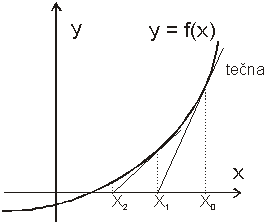
\includegraphics[width=4cm]{matematika/obrazky/newton.png} \end{center}

\newpage
\section{Posloupnosti a řady funkcí}

\begin{pozadavky}
\begin{pitemize}
	\item Spojitost za předpokladu stejnoměrné konvergence
	\item Mocninné řady
	\item Taylorovy řady
	\item Fourierovy řady
\end{pitemize}
\end{pozadavky}

Táto otázka je vypracovaná hlavne podľa skrípt prof. Kalendu, takže je možné že niektoré vety (napr. od prof. Pultra) budú mať iné znenie. Hlavne časť o Fourierových funkciách vyzerá byť prednášaná odlišne (menej obecne)\dots ;-(
\begin{flushright}
\textit{andree}
\end{flushright}

\subsection{Spojitost za předpokladu stejnoměrné konvergence}

\begin{definiceN}{Bodová/stejnoměrná konvergence posloupnosti funkcí}
Řekneme, že posloupnost funkcí $f_n$ \emph{konverguje bodově k funkci $f$ na množině $M$} (značíme $f_n \rightarrow f$), jestliže pro každé  $x \in M$ platí $\lim_{n \rightarrow \infty} f_n(x) = f(x)$, tj. jestliže
$$\forall x \in M\, \forall \varepsilon > 0\, \exists n_0 \in \mathbb{N}\, \forall n \in \mathbb{N}, n \ge n_0: |f_n(x)-f(x)| < \varepsilon$$

Řekneme, že posloupnost $f_n$ \emph{konverguje stejnoměrně k funkci $f$ na množině $M$} (značíme $f_n \rightrightarrows f$), jestliže
$$\forall \varepsilon > 0\, \exists n_0 \in \mathbb{N}\, \forall n \in \mathbb{N}, n \ge n_0\, \forall x \in M: |f_n(x)-f(x)| < \varepsilon$$

Řekneme že posloupnost funkcí je \emph{stejnoměrně konvergentní} na $M$, jestliže konverguje k nějaké funkci na $M$.
\end{definiceN}

\begin{definice}
$\{f_n\}$ \emph{konverguje lokálně stejnoměrně} k funkci $f$ na množině $M$ (značíme $f_n \rightrightarrows^{loc} f$ na $M$), jestliže pro každé $x \in M$ existuje $\varepsilon > 0$ takové, že $f_n \rightrightarrows f$ na $M \cap (x-\varepsilon, x+\varepsilon)$. 
\end{definice}

\begin{vetaN}{Kritérium stejnoměrné konvergence}
Nechť $M$ je (neprázdná) množina, $f$ funkce definovaná na $M$ a $\{f_n\}_{n=1}^{\infty}$ posloupnost funkcí definovaných na $M$. Pak $f_n \rightrightarrows f$, právě když:
$$\lim_{n \rightarrow \infty} \sup\{|f_n(x)-f(x)|; x \in M\} = 0, $$
tj. existuje $n_0 \in \mathbb{N}$ takové, že pro $n \ge n_0$ je $sup\{|f_n(x)-f(x)|; x \in M\}$ definováno (a konečné) a tato posloupnost má limitu 0.
\end{vetaN}

\begin{vetaN}{Bolzano-Cauchyho podmínka pro stejnoměrnou konvergenci}
Nechť $M$ je (neprázdná) množina, $\{f_n\}_{n=1}^{\infty}$ posloupnost funkcí definovaných na $M$. Pak posloupnost $f_n$ je stejnoměrně konvergentní na $M$, právě když:
$$\forall \varepsilon > 0\, \exists n_0 \in \mathbb{N}\, \forall m, n \in \mathbb{N}, m \ge n_0, n \ge n_0\, \forall x \in M: |f_n(x)-f_m(x)| < \varepsilon$$
\end{vetaN}

\begin{vetaN}{O záměně limit, Moore-Osgoodova}
Nechť $a, b \in \mathbb{R}^*, a<b$, $f$ je funkce definovaná na $(a,b)$ a $\{f_n\}_{n=1}^{\infty}$ posloupnost funkcí definovaných na $(a,b)$. Dále nechť $f_n \rightrightarrows f$ na $(a,b)$ a pro každé $n \in \mathbb{N}$ existuje vlastní $\lim_{x \rightarrow a+} f_n(x) = c_n$. Pak existují vlastní limity $\lim_{n \rightarrow \infty} c_n$ a $\lim_{x \rightarrow a+} f(x)$ a platí:
$$\lim_{n \rightarrow \infty} c_n =\lim_{x \rightarrow a+} f(x)$$
Analogicky v bodě $b$ zleva...

\begin{poznamka}
Jiný zápis je, že platí:
$$\lim_{n \rightarrow \infty} \lim_{x \rightarrow a+} f_n(x) = \lim_{x \rightarrow a+} \lim_{n \rightarrow \infty} f_n(x)$$
a navíc jsou tyto limity vlastní, pokud pro každé $n \in \mathbb{N}$ existuje vlastní limita $\lim_{x \rightarrow a+} f_n(x)$ a posloupnost $f_n$ je stejnoměrně konvergentní na $(a,b)$ pro nějaké $b>a$. Tato věta platí i pro \uv{oboustranné} limity.
\end{poznamka}
\end{vetaN}

\begin{vetaN}{Spojitost limitní funkce}
Nechť $I \subset \mathbb{R}$ je interval, f funkce definovaná na $I$ a $\{f_n\}_{n=1}^{\infty}$ posloupnost funkcí definovaných na $I$. Jestliže $f_n$ je spojitá na I pro každé $n \in \mathbb{N}$ a $f_n \rightrightarrows^{loc} f$ na $I$, pak $f$ je spojitá na $I$.
\end{vetaN}

\begin{vetaN}{Záměna limity a derivace}
Nechť $a, b \in \mathbb{R}, a<b$ a $\{f_n\}_{n=1}^{\infty}$ je posloupnost funkcí definovaných na intervalu $(a, b)$, které mají v každém bodě $(a,b)$ vlastní derivaci. Nechť dále platí:
\begin{penumerate}
	\item Existuje takové $x_0 \in (a,b)$, že posloupnost $\{f_n(x_0)\}$ je konvergentní
	\item Posloupnost $\{f_n'\}$ je stejnoměrně konvergentní na $(a,b)$
\end{penumerate}
Pak posloupnost $\{f_n\}$ je stejnoměrně konvergentní na $(a,b)$, a označíme-li $f$ její limitu, pak funkce $f$ má v každém bodě $x \in (a,b)$ vlastní derivaci a platí $f'(x) = \lim_{n \rightarrow \infty} f_n'(x)$.
\end{vetaN}

\begin{definiceN}{Bodová/stejnoměrná konvergence řady funkcí}
Řekneme, že řada $\sum_{n=1}^{\infty} u_n$ \emph{konverguje bodově na množině $M$}, pokud posloupnost jejich částečných součtů je bodově konvergentní na $M$, tj, pro každé $x \in M$ konverguje řada $\sum_{n=1}^{\infty} u_n(x)$.

\emph{Součtem řady} $\sum_{n=1}^{\infty} u_n$ nazveme funkci
$$S(x) = \sum_{n=1}^{\infty} u_n(x) = \lim_{n \rightarrow \infty} s_n(x), \, x \in M,$$
pokud řada konverguje bodově na $M$.

Řekneme, že řada $\sum_{n=1}^{\infty} u_n$ \emph{konverguje stejnoměrně na množině $M$}, pokud posloupnost jejich částečných součtů je stejnoměrně konvergentní na $M$.

Je-li navíc $M \subset \mathbb{R}$, řekneme, že řada $\sum_{n=1}^{\infty} u_n$ \emph{konverguje lokálně stejnoměrně na množině $M$}, pokud posloupnost jejich částečných součtů je lokálně stejnoměrně konvergentní.
\end{definiceN}

\begin{vetaN}{Nutná podmínka stejnoměrné konvergence řady}
Nechť řada $\sum_{n=1}^{\infty} u_n$ konverguje stejnoměrně na množině $M$. Pak $u_n \rightrightarrows 0$ na $M$.
\end{vetaN}

\begin{vetaN}{Srovnávací kritérium pro stejnoměrnou konvergenci}
Nechť M je (neprázdná) množina a $\{u_n\}_{n=1}^{\infty}$, $\{v_n\}_{n=1}^{\infty}$ dvě posloupnosti funkcí definovaných na M, pro které platí $|u_n(x)| \le v_n(x)$ pro všechna $x \in M$. Jestliže řada $\sum_{n=1}^{\infty} v_n$ konverguje stejnoměrně na M, pak i řada $\sum_{n=1}^{\infty} u_n$ konverguje stejnoměrně na $M$.
\end{vetaN}

\begin{vetaN}{Weierstrassovo kritérium}
Nechť $M$ je (neprázdná) množina, $\{u_n\}_{n=1}^{\infty}$ posloupnost funkcí definovaných na $M$ a $\sum_{n=1}^{\infty} c_n$ konvergentní řada reálných čísel. Pokud pro každé $x \in M$ platí $|u_n(x)| \le c_n$, pak řada $\sum_{n=1}^{\infty} u_n$ konverguje stejnoměrně na $M$.
\end{vetaN}

\begin{vetaN}{Leibnizovo kritérium pro stejnoměrnou konvergenci}
Nechť $M$ je (neprázdná) množina, $\{u_n\}_{n=1}^{\infty}$ posloupnost funkcí definovaných na $M$ splňujících \emph{obě} podmínky:

\begin{penumerate}
	\item Pro všechna $x \in M$ a $n \in \mathbb{N}$ je $u_n(x) \ge u_{n+1}(x) \ge 0$
	\item $u_n \rightrightarrows 0$ na $M$
\end{penumerate}
Pak řada $\sum_{n=1}^{\infty} (-1)^{n}u_n$ konverguje stejnoměrně na $M$.
\end{vetaN}

\begin{vetaN}{Dirichletovo a Abelovo kritérium}
Nechť $M$ je (neprázdná) množina a $\{u_n\}_{n=1}^{\infty}$, $\{v_n\}_{n=1}^{\infty}$ dvě posloupnosti funkcí definovaných na $M$, přičemž pro každé $x \in M$ a každé $n \in \mathbb{N}$ platí $v_n(x) \ge v_{n+1}(x) \ge 0$. Nechť navíc platí alespoň jedna z podmínek:
\begin{enumerate}
	\item (Abelovo) Řada $\sum_{n=1}^{\infty} u_n$ konverguje stejnoměrně na M, % a funkce $v_1$ je shora omezená na $M$ -- to je malo, ne? (Tuetschek)
	pro každé pevné $x$ je posloupnost hodnot funkcí $\{v_n(x)\}$ monotónní (klidně pro každé $x$ jinak)
	a existuje $K\in\mathbb{R}$ takové, že $\forall n\in\mathbb{N}\ \forall x\in M: |v_n(x)|<K$ 
	(tj. $\{v_n\}$ je stejnoměrně omezená na $M$). % tahle verze Abelova kriteria je podle Picka a Klazara
	\item (Dirichletovo) Existuje $K \in \mathbb{R}$ takové, že pro všechna $x \in M$ a $n \in \mathbb{N}$ je $|u_1(x) + \dots + u_n(x)| \le K$
	(tj. posloupnost část. součtů $\{\sum_{i=1}^n u_n(x)\}$ je \emph{stejnoměrně omezená} na $M$)
	a dále $v_n \rightrightarrows 0$ na $M$ (konverguje stejnoměrně k nulové funkci).
\end{enumerate}

Pak řada $\sum_{n=1}^{\infty} u_n\cdot v_n$ konverguje stejnoměrně na $M$.
\end{vetaN}

(\emph{Pozn. autora: Dále platí i věty ekvivalentní větám o záměně limit při posloupnostech\dots})

\subsection{Mocninné řady}

\begin{definice}
Nechť $a \in \mathbb{R}$ a $\{c_n\}_{n=0}^{\infty}$ je posloupnost reálných čísel. Nekonečnou řadu funkcí tvaru $\sum_{n=0}^{\infty} c_n(x-a)^n$ nazýváme \emph{mocninnou řadou o středu $a$}.
\end{definice}

\begin{definice}
Nechť $\sum_{n=0}^{\infty} c_n(x-a)^n$ je mocninná řada o středu $a$. Jejím \emph{poloměrem konvergence} rozumíme číslo
$$R = \sup\{r \in \left<0, +\infty\right); \sum_{n=0}^{\infty}|c_n|r^n \textit{konverguje}\}\textrm{,}$$
je-li uvedená množina shora omezená. Není-li shora omezená, klademe $R = +\infty$.
\end{definice}

\begin{veta}
Nechť $\sum_{n=0}^{\infty} c_n(x-a)^n$ je mocninná řada o středu $a$ a $R$ její poloměr konvergence.
\begin{penumerate}
	\item Je-li $|x-a| < R$, pak řada $\sum_{n=0}^{\infty} c_n(x-a)^n$ konverguje absolutně;\\
		Je-li $|x-a| > R$, pak řada $\sum_{n=0}^{\infty} c_n(x-a)^n$ diverguje.
	\item Je-li $r \in (0,R)$, pak řada $\sum_{n=0}^{\infty} c_n(x-a)^n$ konverguje stejnoměrně na množině $\overline{B}(a,r) = \{x \in \mathbb{R}; |x-a|\le r\}=\left<a-r,a+r\right>$.
	\item Řada $\sum_{n=0}^{\infty} c_n(x-a)^n$ konverguje lokálně stejnoměrně na množině $B(a,R) = \{x \in \mathbb{R}; |x-a| < R\}$.
\end{penumerate}

Body 2. a 3. jsou vlastně ekvivalentní. Je-li $R=\infty$, pak řada konverguje lokálně stejnoměrně na celém $\mathbb{R}$. 
\end{veta}

\begin{poznamka}
Množině $B(a, R)$, kde $R$ je poloměr konvergence mocninné řady $\sum_{n=0}^{\infty} c_n(x-a)^n$, se říká \emph{kruh konvergence}.
\end{poznamka}

\begin{vetaN}{Výpočet poloměru konvergence}
Nechť $\sum_{n=0}^{\infty} c_n(x-a)^n$ je mocninná řada o středu $a$ a $R$ její poloměr konvergence.
\begin{penumerate}
	\item Jestliže $L = \limsup_{n \rightarrow \infty} \sqrt[n]{|c_n|}$, pak
		$$R=\left\{ \begin{array}{ll} \frac{1}{L}, & L>0, \\ +\infty, & L=0 \end{array}\right.$$
	\item Týž vzoreček platí, je-li $L = \limsup_{n \rightarrow \infty} \left|\frac{c_{n+1}}{c_n}\right|$
\end{penumerate}
První bod plyne z Cauchyova odmocninového kritéria konvergence řady, druhý z D'Alembertova podílového kritéria. Stejné tvrzení platí i pro limity daných výrazů v případě, že existují.
\end{vetaN}

\begin{vetaN}{...\uv{jen} pomocná pro následující}
Nechť $\sum_{n=0}^{\infty} c_n(x-a)^n$ je mocninná řada o středu $a$ a $R$ její poloměr konvergence. Pak i mocninné řady $\sum_{n=0}^{\infty} n.c_n(x-a)^{n-1}$ a $\sum_{n=0}^{\infty} \frac{c_n}{n+1}(x-a)^{n+1}$ mají poloměr konvergence R.
\end{vetaN}

\begin{vetaN}{Derivace a integrace mocninné řady}
Nechť $\sum_{n=0}^{\infty} c_n(x-a)^n$ je mocninná řada o středu $a$ a $R>0$ její poloměr konvergence. Definujme funkci $f(x) = \sum_{n=0}^{\infty} c_n(x-a)^n, x \in B(a,R)$. Pak platí:
\begin{penumerate}
	\item Funkce $f$ je spojitá na $B(a, R)$.
	\item Funkce $f$ má v každém bodě $x \in B(a,R)$ vlastní derivaci a platí $f'(x) = \sum_{n=0}^{\infty} n\cdot c_n(x-a)^{n-1}$.
	\item Funkce $F(x) = \sum_{n=0}^{\infty} \frac{c_n}{n+1}(x-a)^{n+1}$ je primitivní funkcí k $f$ na $B(a, R)$.
\end{penumerate}
\end{vetaN}


\subsection{Taylorovy řady}

\begin{definice}
Nechť funkce $f$ má v bodě $a$ derivace všech řádů. Pak řadu $\sum_{n=0}^{\infty} \frac{f^{(n)}(a)}{n!}(x-a)^n$ nazýváme \emph{Taylorovou řadou funkce $f$ o středu $a$ v bodě $x$}.
\end{definice}

\begin{poznamka}
Nechť funkce $f$ má v bodě $a$ derivace všech řádů a $x \in \mathbb{R}$. Pak funkce $f$ je v bodě $x$ součtem své Taylorovy řady o středu $a$, právě když $\lim_{n \rightarrow \infty} (f(x) - T_n^a(x))=0$.
\end{poznamka}

\begin{veta}
Nechť $x > a$ a funkce $f$ má v každém bodě intervalu $\left<a,x\right>$ derivace všech řádů. Jestliže platí podmínka
\begin{pitemize}
	\item existuje $C \in \mathbb{R}$ takové, že pro každé $t \in (a,x)$ a každé $n \in \mathbb{N}$ je $|f^{(n)}(t)| \le C$,
\end{pitemize}
pak funkce $f$ je v bodě x součtem své Taylorovy řady o středu $a$. Analogicky pro případ $x < a$.
\end{veta}

\begin{veta}
Nechť $\sum_{n=0}^{\infty} c_n(x-a)^n$ je mocninná řada o středu $a$ a $R>0$ její poloměr konvergence. Definujme funkci $f(x) = \sum_{n=0}^{\infty} c_n(x-a)^n, x \in B(a,R)$. Pak řada $$\sum_{n=0}^{\infty} c_n(x-a)^n$$ je \emph{Taylorovou řadou funkce $f$} o středu $a$, tj. pro každé $n \in \mathbb{N} \cup \{0\}$ platí $c_n = \frac{f^{(n)}(a)}{n!}$.
\end{veta}

\textbf{Význam Taylorových řad}:
\begin{pitemize}
\item aproximace funkcí -- příklady (Taylorovy řady elementárních funkcí):
	$$\forall x \in \mathbb{R}: \exp x=\sum_{k=0}^{\infty} \frac{1}{k!}x^k$$
	$$\forall x \in \mathbb{R}: \sin x=\sum_{k=0}^{\infty} \frac{(-1)^{k-1}}{(2k-1)!}x^{2k-1} \;\;\;\;\dots$$
\item zjednodušení důkazů -- příklad (Důkaz binomické věty): % Zdroj: Pultrova skripta
    \par\medskip
    Rozvineme funkci $f(x)=(1+x)^{\alpha}$ v okolí nuly. Indukcí lze ověřit, že 
    $f^{(k)}(x)=\alpha(\alpha-1)\cdot\dots\cdot(\alpha-k+1)\cdot(1+x)^{\alpha-k}$. 
    Taylorova řada funkce $f(x)=(1+x)^{\alpha}$ konverguje na $(-1,1)$ a je rovna hodnotě $(1+x)^{\alpha}$:
    $$(1+x)^{\alpha}=\sum_{k=0}^{\infty}\frac{\alpha(\alpha-1)\cdot\dots\cdot(\alpha-k+1)}{k!}x^k=\sum_{k=0}^{\infty}\binom{\alpha}{k}x^k$$
    a to dává binomickou větu.
\end{pitemize}

\subsection{Fourierovy řady}

\subsubsection{Obecné Fourierovy řady}

\begin{definice}
Nechť $\{\varphi_n\}_{n=1}^{\infty}$ je posloupnost komplexních funkcí na $\left<a,b\right>$, z nichž žádná není konstantně nulová. Řekneme, že tato posloupnost tvoří \emph{ortogonální (krátce OG) systém na $\left<a,b\right>$}, jestliže pro každá dvě různá $m, n\in \mathbb{N}$ platí:
$$\int_a^b \varphi_m \overline{\varphi_n} = 0$$
Pokud navíc
$$\int_a^b |\varphi_n|^2= 1$$
pro všechna $n \in \mathbb{N}$, říkáme, že jde o \emph{ortonormální systém}.
\end{definice}

\begin{poznamka}
Příklady OG systémů:
\begin{pitemize}
	\item Systém tvořený funkcemi $\exp \frac{2k\pi i x}{p}, k \in \mathbb{Z}$ je OG na intervalu $\left<a, a+p\right>$ pro každé $a \in \mathbb{R}$
	\item Systém tvořený funkcemi $1, \cos \frac{2k\pi x}{p}, \sin \frac{2k\pi x}{p}, k \in \mathbb{N}$ je OG na intervalu \par$\left<a, a+p\right>$ pro každé $a \in \mathbb{R}$
\end{pitemize}
\end{poznamka}

\begin{veta}
Nechť $\{\varphi_n\}_{n=1}^{\infty}$ je posloupnost komplexních funkcí na $\left<a,b\right>$, $\{a_n\}_{n=0}^{\infty}$ je posloupnost komplexních čísel. Jestliže
$$f(x) = \sum_{n=1}^{\infty} a_n \varphi_n(x), \, x \in \left<a,b\right>,$$
a uvedená řada konverguje stejnoměrně na $\left<a,b\right>$, pak pro každé $n \in \mathbb{N}$ platí
$$a_n = \frac{\int_a^b f\overline{\varphi_n}}{\int_a^b |\varphi_n|^2}.$$
\end{veta}

\begin{definiceN}{po částech spojitá funkce}
Řekneme, že funkce $f$ je \emph{po částech spojitá na $\left<a,b\right>$}, jestliže existuje $D=\{x_i\}_{j=0}^{N}$ dělení intervalu $\left<a,b\right>$ takové, že pro každé $j \in \{1,\dots,N\}$ je funkce $f$ spojitá na intervalu $(x_{j-1}, x_j)$ a v krajních bodech tohoto intervalu má vlastní jednostranné limity.
\end{definiceN}

\begin{definice}
Nechť $\{\varphi_n\}_{n=1}^{\infty}$ je OG systém na $\left<a,b\right>$ a funkce $f$ je po částech spojitá na $\left<a,b\right>$. Pro $n \in \mathbb{N}$ položme
$$a_n = \frac{\int_a^b f\overline{\varphi_n}}{\int_a^b |\varphi_n|^2}.$$
Tato čísla nazýváme \emph{Fourierovými koeficienty funkce $f$ vzhledem k OG systému $\{\varphi_n\}_{n=1}^{\infty}$ na $\left<a,b\right>$} a řadu
$$\sum_{n=1}^{\infty} a_n \varphi_n$$
nazýváme \emph{Fourierovou řadou $f$ vzhledem k OG systému $\{\varphi_n\}_{n=1}^{\infty}$ na $\left<a,b\right>$}.
\end{definice}

\subsubsection{Trigonometriké Fourierovy řady}

\begin{definiceN}{po částech spojitá periodická funkce}
Buď funkce $f$ periodická s periodou $p > 0$. Řekneme, že je \emph{po částech spojitá}, je-li po částech spojitá na intervalu $\left<0,p\right>$.
\end{definiceN}

\begin{poznamka}
Nechť $f$ je $p$-periodická funkce a $a,b \in \mathbb{R}$.
\begin{penumerate}
	\item Pak $f$ je počástech spojitá na $\left<a, a+p\right>$, právě když je po částech spojitá na $\left<b, b+p\right>$.
	\item $\int_a^{a+p}f = \int_b^{b+p}f$, pokud alespoň jeden z těchto integrálů existuje.
\end{penumerate}
\end{poznamka}

\begin{definice}
Nechť funkce $f$ je $p$-periodická po částech spojitá funkce. Jejími \emph{trigonometrickými Fourierovými koeficienty} rozumíme čísla
$$a_n = \frac{2}{p} \int_0^p f(x)\cos \frac{2\pi nx}{p}dx, \, n \in \mathbb{N} \cup \{0\}$$
$$b_n = \frac{2}{p} \int_0^p f(x)\sin \frac{2\pi nx}{p}dx, \, n \in \mathbb{N}$$
\end{definice}

\begin{definice}
\emph{Trigonometrickou Fourierovou řadou} funkce $f$ pak rozumíme řadu
$$\frac{a_0}{2} + \sum_{n=1}^{\infty} \left( a_n \cos \frac{2\pi nx}{p} + b_n \sin \frac{2\pi nx}{p}\right)$$
\end{definice}

\begin{poznamkaN}{Besselova nerovnost}
Besselova nerovnost pro trigonometrické Fourierovy řady má tvar
$$\frac{|a_0|^2}{4}p + \sum_{n=1}^{\infty} (|a_n|^2 + |b_n|^2)\frac{p}{2} \le \int_0^p |f|^2.$$
Podobná nerovnost platí i pro obecné Fourierovy řady.
\par\medskip\noindent
(Riemann-Lebesgue) důsledkem této nerovnosti je fakt, že $\lim a_n = \lim b_n = 0$.
\end{poznamkaN}

\begin{vetaN}{Persevalova rovnost}
Pro trigonometrické Fourierovy řady platí v Besselově nerovnosti rovnost. Pro funkce s periodou $2\pi$ potom platí:
$$\frac{1}{\pi} \int_{-\pi}^{\pi} |f|^2= \frac{|a_0|^2}{2}+\sum_{n=1}^{\infty} (|a_n|^2 + |b_n|^2) \,\,\,\textit{(jedna z variant zápisu)}$$
\end{vetaN}

\begin{poznamka}
Nechť $f$ je $p$-periodická po částech spojitá funkce taková, že všechny její trigonometrické Fourierovy koeficienty jsou nulové. Pak $f(x)=0$ pro všechna $x \in \left<0,p\right>$ s výjimkou konečně mnoha bodů.
\end{poznamka}

\begin{vetaN}{Symetrie funkce a Trigonometrické Fourierovy koeficienty}
Nechť $f$ je $p$-periodická po částech spojitá funkce, $a_n, n \in \mathbb{N} \cup \{0\}$ a $b_n, n \in \mathbb{N}$, její trigonometrické Fourierovy koeficienty. Pak platí
\begin{penumerate}
	\item Pro všechna $n \in \mathbb{N} \cup \{0\}$ je $a_n=0$, právě když $f(-x) = -f(x)$ pro všechna $x \in \left<0,p\right>$ s výjimkou konečně mnoha bodů.
	\item Pro všechna $n \in \mathbb{N}$ je $b_n=0$, právě když $f(-x) = f(x)$ pro všechna $x \in \left<0,p\right>$ s výjimkou konečně mnoha bodů.
\end{penumerate}
\end{vetaN}

\begin{definice}
Nechť $f$ je $p$-periodická po částech spojitá funkce. Řekneme, že $f$ je \emph{po částech hladká}, jestliže $f'$ je po částech spojitá.
\end{definice}

\begin{vetaN}{O konvergenci Fourierových řad}
Nechť $f$ je po částech hladká p-periodická funkce. Pak platí:
\begin{penumerate}
	\item Trigonometrická Fourierova řada funkce $f$ konverguje bodově na $\mathbb{R}$ a její součet v bodě $x \in \mathbb{R}$ je $\frac{1}{2} \left( \lim_{t\rightarrow x-} f(t) + \lim_{t\rightarrow x+} f(t)\right)$
	\item Je-li $f$ navíc spojitá na intervalu $(a,b)$, pak její trigonometrická Fourierova řada konverguje lokálně stejnoměrně na $(a,b)$ a její součet je $f(x)$ pro každé $x \in (a,b)$.
	\item Je-li navíc spojitá na $\mathbb{R}$, pak její trigonometrická Fourierova řada konverguje stejnoměrně na $\mathbb{R}$ a její součet je $f(x)$ pro každé $x \in \mathbb{R}$.
\end{penumerate}
\end{vetaN}

% derivacia FR?: podle me netreba, ani Pick ani Klazar ani Pultr to nemaji ve skriptech / neprednaseli -- Tuetschek

\newpage
\def\d{\mathrm{d}}
\def\vol{\mathrm{vol\ }}


\section{Integrál}

\begin{pozadavky}
\begin{pitemize}
	\item Primitivní funkce, metody výpočtu
	\item Určitý (Riemannův) integrál, užití určitého integrálu
	\item Vícerozměrný integrál a Fubiniho věta
\end{pitemize}
\end{pozadavky}

\subsection{Primitivní funkce, metody výpočtu}

\begin{definice}
Nechť funkce $f$ je definována na otevřeném intervalu $I$. Řekneme, že funkce $F$ je \emph{primitivní funkce k $f$ na $I$}, jestliže pro každé $x \in I$ existuje $F'(x)$ a platí $F'(x)=f(x)$.
\end{definice}

\begin{vetaN}{Tvar primitivní funkce}
Nechť $F$ a $G$ jsou dvě primitivní funkce k funkci $f$ na otevřeném intervalu $I$. Pak existuje $c \in \mathbb{R}$ tak, že $F(x)=G(x)+c$ pro každé $x \in I$.
\end{vetaN}

\begin{vetaN}{Linearita primitivní funkce}
Nechť f má na otevřeném intervalu $I$ primitivní funkci $F$, funkce $g$ má na na $I$ primitivní funkci $G$ a $\alpha, \beta \in \mathbb{R}$. Potom funkce $\alpha F + \beta G$ je primitivní funkcí k $\alpha f + \beta g$ na $I$.

\begin{poznamka}
Předchozí tvrzení často zapisujeme (pokud alespoň jedno z čísel $\alpha, \beta$ je různé od nuly)
$$\int (\alpha f(x) + \beta g(x)) \d x = \alpha \int f(x) \d x + \beta \int g(x) \d x.$$
\end{poznamka}
\end{vetaN}

\begin{vetaN}{Spojitost a existence primitivní funkce}
Nechť $f$ je spojitá funkce na otevřeném intervalu $I$. Pak $f$ má na $I$ primitivní funkci.
\end{vetaN}

\begin{vetaN}{O substituci}
\begin{penumerate}
\item Nechť $F$ je primitivní funkce k $f$ na $(a,b)$. Nechť $\varphi$ je funkce definována na $(\alpha, \beta)$ s hodnotami v intervalu $(a,b)$, která má v každém bodě $t \in (\alpha, \beta)$ vlastní derivaci. Pak
$$\int f(\varphi(t))\varphi'(t)dt=F(\varphi(t))+C \textit{ na } (\alpha,\beta)$$
\item Nechť funkce $\varphi$ má v každém bodě intervalu $(\alpha,\beta)$ nenulovou vlastní derivaci a $\varphi((\alpha,\beta)) = (a,b)$. Nechť funkce $f$ je definována na intervalu $(a,b)$ a platí
$$\int f(\varphi(t))\varphi'(t)dt=G(t)+C \textit{ na } (\alpha,\beta)$$
Pak
$$\int f(x)\d x=G(\varphi^{-1}(x))+C \textit{ na } (a,b)$$
\end{penumerate}
\end{vetaN}

\begin{vetaN}{Integrace per partes}
Nechť $I$ je otevřený interval a funkce $f$ a $g$ jsou spojité na $I$. Nechť $F$ je primitivní funkce k $f$ na $I$ a $G$ je primitivní funkce ke $g$ na $I$. Pak platí
$$\int g(x)F(x)\d x=G(x)F(x) - \int G(x)f(x)\d x \textit{ na } I$$

(\emph{Poznámka autora}: $\int u'v = uv - \int uv'$)
\end{vetaN}

\subsubsection{Postup integrace racionální funkce}

\begin{vetaN}{Dělení polynomu}
Nechť P a Q jsou polynomy s reálnými koeficienty, přičemž Q není identicky roven nule. Pak existují (jednoznačně určené) polynomy R a S takové, že stupeň S je menší než stupeň Q a pro všechna $x \in \mathbb{R}$ platí $P(x)=R(x)Q(x)+S(x)$.
\end{vetaN}

\begin{vetaN}{Základní věta algebry}
Nechť $P(x)=a_nx^n+\dots+a_1x+a_0$ je polynom stupně $n$ s reálnými koeficienty. Pak existují čísla $x_1,\dots,x_n \in \mathbb{C}$ taková, že
$$P(x)=a_n(x-x_1)\dots(x-x_n), \,\, x \in \mathbb{R}$$
\end{vetaN}

\begin{vetaN}{O kořenech polynomu}
Nechť $P$ je polynom s reálnými koeficienty a $z \in \mathbb{C}$ je kořen $P$ násobnosti $k \in \mathbb{N}$. Pak i $\overline{z}$ je kořen $P$ násobnosti k.
\end{vetaN}

\begin{vetaN}{O rozkladu polynomu}
Nechť $P(x)=a_nx^n +\dots+a_1x+a_0$ je polynom stupně $n$ s reálnými koeficienty. Pak existují reálná čísla $x_1,\dots,x_k,\alpha_1,\dots,\alpha_l,\beta_1,\dots,\beta_l$ a přirozená čísla $p_1,\dots,p_k,q_1,\dots,q_l$ taková, že:

\begin{penumerate}
	\item $P(x)=a_n(x-x_1)^{p_1} \dots (x-x_k)^{p_k}(x^2+\alpha_1x+\beta_1)^{q_1}\dots(x^2+\alpha_lx+\beta_l)^{q_l}$,
	\item žádné dva z mnohočlenů $x-x_1,x-x_2,\dots,x-x_k,x^2+\alpha_1x+\beta_1,\dots,x^2+\alpha_lx+\beta_l$ nemají společný kořen,
	\item mnohočleny $x^2+\alpha_1x+\beta_1,\dots,x^2+\alpha_lx+\beta_l$ nemají žádný reálný kořen.
\end{penumerate}
\end{vetaN}

\begin{vetaN}{O rozkladu na parciální zlomky}
Nechť $P,Q$ jsou polynomy s reálnými koeficienty takové, že

\begin{penumerate}
	\item stupeň $P$ je ostře menší než stupeň $Q$,
	\item $Q(x)=a_n(x-x_1)^{p_1}\dots(x-x_k)^{p_k} (x^2+\alpha_1x+\beta_1)^{q_1}\dots(x^2+\alpha_lx+\beta_l)^{q_l}$,
	\item $a_n,x_1,\dots,x_k,\alpha_1,\dots,\alpha_l,\beta_1,\dots,\beta_l \in \mathbb{R}, a_n \neq 0$
	\item $p_1,\dots,p_k,q_1,\dots,q_l \in \mathbb{N}$
	\item žádné dva z mnohočlenů $x-x_1, x-x_2,\dots,x-x_k,x^2+\alpha_1x+\beta_1,\dots,x^2+\alpha_lx+\beta_l$ nemají společný kořen
	\item mnohočleny $x^2+\alpha_1x+\beta_1, \dots, x^2+\alpha_lx+\beta_l$ nemají reálný kořen
\end{penumerate}

Pak existují jednoznačně určená čísla $A_1^1,\dots,A_{p_1}^{1},\dots,A_1^k,\dots,A_{p_k}^k,\\B_1^1,C_1^1,\dots,B_{q_1}^1,C_{q_1}^{1},\dots,B_1^l,C_1^l,\dots,B_{q_l}^l,C_{q_l}^l$ taková, že platí


\begin{align*}
\frac{P(x)}{Q(x)} & = \frac{A_1^1}{(x-x_1)^{p_1}} + \dots + \frac{A_{p_1}^1}{(x-x_1)} + \dots + \frac{A_1^k}{(x-x_k)^{p_k}} + \dots + \frac{A_{p_k}^k}{(x-x_k)}\\
&+ \frac{B_1^1x+C_1^1}{(x^2+\alpha_1x+\beta_1)^{q_1}} + \dots + \frac{B_{q_1}^1x+C_{q_1}^1}{x^2+\alpha_1x+\beta_1} + \dots\\
&+ \frac{B_1^lx+C_1^l}{(x^2+\alpha_lx+\beta_l)^{q_l}} + \dots + \frac{B_{q_l}^lx+C_{q_l}^l}{x^2+\alpha_lx+\beta_l}.
\end{align*}

\end{vetaN}

\textbf{Postup integrace racionální funkce $\frac{P(x)}{Q(x)}$ je:}
\begin{penumerate}
\item Vydělíme polynomy $P$ a $Q$ - najdeme polynomy $R$ a $S$ takové, že
	$$\frac{P(x)}{Q(x)} = R(x) + \frac{S(x)}{Q(x)}$$
	a stupeň S je menší než stupeň Q.

\item Najdeme rozklad polynomu Q ve tvaru uvedeném ve \emph{větě o rozkladu polynomu}.

\item Najdeme rozklad $\frac{S}{Q}$ na parciální zlomky ve tvaru uvedeném ve \emph{větě o rozkladu na parciální zlomky}.

\item Najdeme primitivní funkce ke všem parciálním zlomkům.
\end{penumerate}

\subsection{Určitý (Riemannův) integrál, užití určitého integrálu}

\begin{definice}
Konečnou posloupnost $D=\{x_j\}_{j=0}^n$ nazýváme \emph{dělením intervalu} $\left<a,b\right>$, jestliže platí
$$a=x_0 < x_1 < \dots < x_n = b$$

Body $x_0,\dots,x_n$ nazýváme dělícími body. \emph{Normou dělení} $D$ rozumíme číslo
$$\upsilon(D)=\max\{x_j-x_{j-1}; j=1,\dots,n\}.$$

Řekneme, že dělení $D'$ intervalu $\left<a,b\right>$ je \emph{zjemněním dělení} $D$ intervalu $\left<a,b\right>$, jestliže každý dělící bod $D$ je i dělícím bodem $D'$.
\end{definice}

\begin{definice}
Nechť $f$ je omezená funkce definovaná na intervalu $\left<a,b\right>$ a $D=\{x_j\}_{j=0}^n$ je dělení $\left<a,b\right>$. Označme
$$S(f,D)=\sum_{j=1}^{n} M_j(x_j-x_{j-1}), \textit{ kde } M_j=\sup\{f(x); x\in \left<x_{j-1},x_j\right>\}$$
$$s(f,D)=\sum_{j=1}^{n} m_j(x_j-x_{j-1}), \textit{ kde } m_j=\inf\{f(x); x\in \left<x_{j-1},x_j\right>\}$$

\begin{poznamka}
Nechť $f$ je omezená funkce definovaná na intervalu $\left<a,b\right>$.
\begin{penumerate}
	\item Pro každé dělaní $D$ intervalu $\left<a,b\right>$. platí $s(f,D)\le S(f,D)$.
	\item Je-li $D_1$ zjemněním $D_2$, pak $s(f,D_1) \ge s(f,D_2)$ a $S(f,D_1) \le S(f, D_2)$
	\item Jsou-li $D_1$ a $D_2$ dělení intervalu $\left<a,b\right>$, pak $s(f,D_1) \le S(f, D_2)$.
\end{penumerate}
\end{poznamka}
\end{definice}

\begin{definice}
Nechť $f$ je omezená funkce definovaná na intervalu $\left<a,b\right>$.
\begin{penumerate}
\item
Označme
$$\overline{\int_a^b}f=\inf\{S(f,D); D \textit{ je dělením intervalu } \left<a,b\right>\}$$
\begin{center}(tzv. horní \emph{Riemannův integrál funkce} $f$ přes $\left<a,b\right>$),\end{center}

$$\underline{\int_a^b}f=\sup\{s(f,D); D \textit{ je dělením intervalu } \left<a,b\right>\}$$
\begin{center}(tzv. dolní \emph{Riemannův integrál funkce} $f$ přes $\left<a,b\right>$)\end{center}

\item Řekneme, že funkce $f$ má \emph{Riemannův integrál přes} $\left<a,b\right>$, pokud $\overline{\int_a^b}f=\underline{\int_a^b}f$. Hodnota tohoto integrálu je pak rovna $\overline{\int_a^bf}$ a značíme ji $\int_a^bf$. 

Pokud $a>b$, definujeme $\int_a^bf=-\int_b^af$, v případě, že $a=b$, definujeme $\int_a^b=0$.
\end{penumerate}
\end{definice}

\begin{vetaN}{Kritérium existence Riemannova integrálu}
Nechť $a<b$ a $f$ je funkce omezená na $\left<a,b\right>$. Pak $\int_a^bf$ existuje, právě když pro každé $\varepsilon > 0$ existuje dělení $D$ intervalu $\left<a,b\right>$ takové, že $S(f,D)-s(f,D)<\varepsilon$
\end{vetaN}

\begin{vetaN}{Monotonie a linearita Riemannova integrálu}
Nechť $a,b\in \mathbb{R}, a<b$ a funkce $f,g$ mají Riemannův integrál přes interval $\left<a,b\right>$. Pak platí:
\begin{penumerate}
	\item Jestliže pro každé $x \in \left<a,b\right>$ je $f(x) \le g(x)$, pak $\int_a^bf \le \int_a^bg$
	\item $\int_a^b(f+g) = \int_a^bf + \int_a^bg$
	\item $\int_a^bcf=c\int_a^bf$ pro každé $c \in \mathbb{R}$
\end{penumerate}
\end{vetaN}

\begin{vetaN}{Spojitost a Riemannovská integrovatelnost}
Nechť $a,b\in \mathbb{R}, a<b$ a funkce $f$ je spojitá na intervalu $\left<a,b\right>$. Pak existuje $\int_a^bf$.
\begin{poznamka}
Platí dokonce: Pokud je $f$ omezená na $\left<a,b\right>$ a je spojitá ve všech bodech intervalu $\left<a,b\right>$ s výjimkou konečně mnoha, pak existuje $\int_a^bf$.
\end{poznamka}
\end{vetaN}


\begin{vetaN}{Monotonie a Riemannovská integrovatelnost}
Je li $f$ omezená a monotónní na uzavřeném intervalu, pak je Riemannovsky integrovatelná. % Proc ty otazniky? to plati. -- Tuetschek
\end{vetaN}

\begin{vetaN}{Vlastnosti $\int$}
Nechť $a,b\in \mathbb{R}, a<b$ a funkce $f$ je omezená na intervalu $\left<a,b\right>$. Pak platí
\begin{penumerate}
	\item Jestliže existuje $\int_a^bf$, pak pro každý interval $\left<c,d\right> \subset \left<a,b\right>$ existuje $\int_c^df$.
	\item Je-li $c \in (a,b)$, pak $\int_a^bf=\int_a^cf+\int_c^bf$, má-li alespoň jedna strana smysl (\emph{aditivita Riemannova integrálu jako funkce intervalu})
\end{penumerate}
\end{vetaN}

\begin{vetaN}{Riemannův integrál jako primitivní funkce}
Nechť $a,b\in \mathbb{R}, a<b$ a funkce $f$ je omezená na intervalu $\left<a,b\right>$. Pro $x \in \left<a,b\right>$ položme $F(x)=\overline{\int_a^x}f$. Potom platí:
\begin{penumerate}
	\item Funkce $F$ je spojitá na $\left<a,b\right>$
	\item Je-li $x_0 \in (a,b)$ a funkce $f$ je v bodě $x_0$ spojitá, pak $F'(x_0)=f(x_0)$.
\end{penumerate}
Stejná tvrzení platí i pro funkci $G(x)=\underline{\int_a^x}f$
\end{vetaN}

\begin{poznamka}
Pro Riemannovy integrály lze použít i metodu per partes nebo pravidlo substituce. % tohle by mozna chtelo formulovat nejak formalneji -- Tuetschek
\end{poznamka}


\begin{vetaN}{Základní věta analýzy}
Nechť $a,b\in \mathbb{R}, a<b$ a funkce $f$ je spojitá na intervalu $\left<a,b\right>$. Nechť $F$ je primitivní funkce k $f$ na intervalu $(a,b)$. Pak existují vlastní limity $\lim_{x\rightarrow a+}F(x)$ a $\lim_{x\rightarrow b-}F(x)$ a platí:
$$\int_a^bf = (\lim_{x\rightarrow b-}F(x))-(\lim_{x\rightarrow a+}F(x))$$
\end{vetaN}


\begin{definiceN}{Newtonův integrál}
Nechť funkce $f$ je definována na intervalu $(a,b)$ a $F$ je primitivní funkce k $f$ na $(a,b)$. \emph{Newtonovým integrálem} funkce $f$ přes interval $(a,b)$ nazýváme číslo
$$(N)\int_a^bf = (\lim_{x\rightarrow b-}F(x))-(\lim_{x\rightarrow a+}F(x))$$
pokud obě limity na pravé straně existují a jsou vlastní.
\end{definiceN}

\begin{poznamkaN}{Vztah Riemannova a Newtonova integrálu}
Je-li funkce $f$ spojitá na intervalu $\left<a,b\right>$, pak platí: 
$$(N)\int_a^b f(x) \d x = (R)\int_a^b f(x) \d x$$

Množiny funkcí integrovatelných newtonovsky a riemannovsky jsou neporovnatelné.
\end{poznamkaN}


\subsubsection{Užití určitého integrálu}

Obsahy rovinných útvarů...

\begin{vetaN}{Délka křivky}
Nechť $f$ má na $(a,b)$ spojitou derivaci. Délka křivky v $\mathbb{R}^2$, vyznačené průběhem funkce $f$ z $[a;f(a)]$ do $[b;f(b)]$ potom je dána předpisem:
$$L(f)=\int_a^b \sqrt{1+(f'(x))^2}\d x.$$
\end{vetaN}

\begin{vetaN}{Objem rotačního tělesa}
Nechť $f$ je definována na $\left<a,b\right>$ a $f>0$. Objem tělesa vzniknutého rotací křivky je $V=\pi \int_a^bf(x)^2\d x$
\end{vetaN}

\begin{vetaN}{Integrální kritérium konvergence řad}
Nechť $f$ je spojitá, nezáporná a nerostoucí na $\left<n_0-1,\infty\right)$, kde $n_0 \in \mathbb{N}$. Potom

$$\sum_{n=1}^{\infty} f(n) \textit{ konverguje} \Leftrightarrow (N)\int_{n_0}^{\infty}f(t)dt < \infty$$
\end{vetaN}

\subsection{Vícerozměrný integrál a Fubiniho věta}

\begin{definice}
(Kompaktním) \emph{intervalem} v $n$-rozměrném euklidovském prostoru $E_n$ rozumíme součin
$$J = \left<a_1,b_1\right> \times \dots \times \left<a_n,b_n\right>$$
kde $\left<a_i,b_i\right>$ jsou kompaktní intervaly v $\mathbb{R}$.
\end{definice}

\begin{definice}
\begin{pitemize}
\item \emph{Rozdělením} $D$ takového intervalu $J$ rozumíme $n$-tici $D_1, \dots, D_n$, kde $D_i$ je rozdělení intervalu $\left<a_i,b_i\right>$.
\item Rozdělení $D=(D_1,\dots,D_n)$ je \emph{zjemněním} $D'=(D'_1,\dots,D'_n)$ jestliže $D_i$ zjemňuje $D'_i$.
\end{pitemize}
\end{definice}

\begin{pozorovani}
Každé dvě rozdělení mají společné zjemnění.
\end{pozorovani}

\begin{definice}
\emph{Člen rozdělení} $D=(D_1,\dots,D_n)$ je kterýkoliv interval $K=\left<t_{1, i_1}, t_{1, i_1+1}\right> \times \dots \times \left<t_{n, i_n}, t_{n, i_n+1}\right>$, kde $D_k: t_{k0} < \dots < t_{k,r(k)}, \, \, 0 \le i_j \le r(j)$. Množina všech členů rozdělení $D$ bude označována $|D|$. % urcite tu melo byt podrozdeleni?? -- Tuetschek
\end{definice}

\begin{definice}
\emph{Objem intervalu} $J=\left<a_1,b_1\right> \times \dots \times \left<a_n,b_n\right>$ je číslo
$$\vol J=(b_1-a_1).(b_2-a_2)\dots(b_n-a_n)$$
\end{definice}

\begin{definice}
Buď $f$ omezená funkce na intervalu $J$, buď $D$ rozdělení $J$. \emph{Dolní (resp. horní) sumou} funkce $f$ v rozdělení $D$ rozumíme číslo
$$s(f,D)=\sum_{K\in |D|}m_K\cdot\vol K \textit{\;\;resp.\;\;} S(f,D) = \sum_{K \in |D|} M_K\cdot\vol K,$$
kde $m_K$ je infimum a $M_k$ supremum funkce $f$ na intervalu $K$.
\end{definice}

\begin{pozorovani}
Pro libovolná dvě rozdělení $D$ a $D'$ platí $s(f,D) \le S(f,D')$
\end{pozorovani}

\begin{definice}
Dolní a horní Riemannův integrál definujeme jako
$$\underline{\int}_Jf=\sup_Ds(f,D), \;\;\; \overline{\int}_Jf=\inf_DS(f,D)$$
a při rovnosti těchto hodnot mluvíme o Riemannově integrálu a píšeme prostě
$$\int_Jf \textit{ nebo } \int_Jf(x_1,\dots,x_n)\d x_1\dots x_n, \;\;\;\int_Jf(\overrightarrow{x})d\overrightarrow{x}.$$
\end{definice}

\begin{veta}
Pro vícerozměrný Riemannův integrál platí (podobně jako pro jednorozměrný případ) že $f$ je Riemannovsky integrovatelná, právě když ke každému $\varepsilon > 0$ existuje rozdělení $D$ takové, že
$$S(f,D)-s(f,D)<\varepsilon$$

Platí i věta, že spojitá funkce na intervalu $J$ je Riemannovsky integrovatelná.
\end{veta}

\begin{vetaN}{Vlastnosti Riemannova vícerozměrného integrálu}
Platí:
\begin{penumerate}
	\item $|\int_J f| \le \int_J|f|$ (existují-li příslušné integrály)
	\item Buďte $f,g$ Riemannovsky integrovatelné funkce na $J$, buď $f \le g$. Potom $\int_J f \le \int_J g$.
	\item Speciálně, je-li $f(\overrightarrow{x})\le C$ pro nějakou konstantu $C$, platí $\int_J f \le C\cdot \vol J$
\end{penumerate}
\end{vetaN}

\begin{vetaN}{Fubiniova}
Buďte $J' \subseteq E^n, J'' \subseteq E^m$ intervaly, $J=J' \times J''$, buď $f$ spojitá funkce definovaná na $J$. Potom
$$\int_J f(\overrightarrow x,\overrightarrow y)d\overrightarrow x\overrightarrow y =
\int_{J'}\left(\int_{J''}f(\overrightarrow x,\overrightarrow y)d\overrightarrow y\right)d\overrightarrow x =
\int_{J''}\left(\int_{J'}f(\overrightarrow x,\overrightarrow y)d\overrightarrow x\right)d\overrightarrow y
$$

(Inými slovami: Hodnota \uv{integrálu} cez celý interval je rovná hodnote po integrovaní postupne cez (jednotlivé) \uv{rozmery} - pričom je možné integrovať v ľubovoľnom poradí.)
\end{vetaN}

\begin{definiceN}{Parciální derivace}
\emph{Parciální derivace} funkce $f$ v bodě $a\in\mathbb{R}^n$ podle proměnné $x_i$ se definuje následovně:
$$\frac{\partial f}{\partial x_i}(a)=\lim_{h\to 0}\frac{f(a_1,\dots,a_{i-1},a_i + h,a_{i+1},\dots,a_n)-f(a_1,\dots,a_n)}{h}$$
\end{definiceN}

\begin{definiceN}{Jacobiho matice, jakobián}
\emph{Jacobiho matice} funkce $\overrightarrow f:D\to \mathbb{R}^n$ v bodě $a\in D$, kde $D$ je otevřená množina v $\mathbb{R}^m$ a $f_1,f_2,\dots f_n$ jsou souřadnicové funkce $f$, je dána předpisem:
$$
\left(\frac{\partial f_i}{\partial x_j}(a)\right)_{i,j=1}^{n,m} =
\left( \begin{matrix}
	\frac{\partial f_1}{\partial x_1} & \cdots & \frac{\partial f_1}{\partial x_m} \\
	\vdots & \ddots & \vdots \\
	\frac{\partial f_n}{\partial x_1} & \cdots & \frac{\partial f_n}{\partial x_m}
\end{matrix} \right)
$$

\noindent Táto čtvercová matice se obvykle značí $\frac{D(f_1,\dots,f_n)}{D(x_1,\dots,x_n)}$ -- a je-li $m=n$, její determinant se nazývá \emph{Jakobián} (a značí se rovnako???).
\end{definiceN}

\begin{definiceN}{Regulární zobrazení}
Nechť $U \subseteq \mathbb{R}^n$ je otevřená množina, $\overrightarrow f: U \rightarrow \mathbb{R}^n$ má spojité parciální derivace. \emph{Zobrazení $\overrightarrow f$ je regulární}, je-li jakobián
$$\frac{D(f_1,\dots,f_n)}{D(x_1,\dots,x_n)}(\overrightarrow x) \neq 0, \,\, \forall \overrightarrow x \in U$$
\end{definiceN}


\begin{vetaN}{O substituci}
Nechť $\varphi: U \subseteq \mathbb{R}^n \rightarrow \mathbb{R}^n$ je regulární zobrazení, $A$ je uzavřená množina v $\mathbb{R}^n$, $A \subseteq U$ na které existuje $\int_{\varphi(A)}f(\overrightarrow x)d\overrightarrow x$. Potom platí:
$$\int_A f(\overrightarrow{\varphi}(\overrightarrow t)) \frac{D(\overrightarrow \varphi)}{D(\overrightarrow t)}d\overrightarrow t = \int_{\varphi (A)} f(\overrightarrow x)d\overrightarrow x$$
\end{vetaN}

\newpage
\section{Základy teorie funkcí více proměnných}

\begin{pozadavky}
\begin{pitemize}
	\item Parciální derivace a totální diferenciál
	\item Věty o střední hodnotě
	\item Extrémy funkcí více proměnných
	\item Věta o implicitních funkcích
\end{pitemize}
\end{pozadavky}

\subsection{Parciální derivace a totální diferenciál}

\begin{definiceN}{Parciální derivace}
Nechť $f: \mathbb{R}^n \rightarrow \mathbb{R}$, $t \in \mathbb{R}$, $X = [x_1, \ldots, x_n], X \in \mathbb{R}^n$. Potom \textit{parciální derivací funkce $f$ podle i-té složky v bodě X} nazveme limitu
$$\frac{\partial f}{\partial x_i}(X) = \displaystyle\lim_{t \rightarrow 0}~\frac{f(x_1,\ldots,x_i + t,\ldots,x_n) - f(x_1,\ldots,x_n)}{t}$$
pokud tato limita existuje a je vlastní.
\end{definiceN}

\begin{definiceN}{Derivace ve směru vektoru}
Nechť $f: \mathbb{R}^n \rightarrow \mathbb{R}$, $v \in \mathbb{R}^n\setminus\{0^n\}$, $X = [x_1, \ldots, x_n], X \in \mathbb{R}^n$. Potom \textit{derivací funkce $f$ ve směru vektoru v} nazveme limitu
$$D_vf(X) = \displaystyle\lim_{t \rightarrow 0}~\frac{f(X + t \cdot v) - f(X)}{t}$$
pokud tato limita existuje a je vlastní.
\end{definiceN}

\begin{definiceN}{Gradient}
Nechť $f: \mathbb{R}^n \rightarrow \mathbb{R}$, $X = [x_1, \ldots, x_n], X \in \mathbb{R}^n$ a nechť existují všechny parciální derivace funkce $f$ v bodě $X$ a jsou vlastní. Pak vektor $\nabla f(X) = [\frac{\partial f}{\partial x_1}(X),\ldots,\frac{\partial f}{\partial x_n}(X)]$ nazýváme \textit{gradientem funkce $f$ v bodě $X$}.
\end{definiceN}

\begin{definiceN}{Totální diferenciál}
Nechť $f: \mathbb{R}^n \rightarrow \mathbb{R}$, $X = [x_1, \ldots, x_n], X \in \mathbb{R}^n$ a nechť $v \in \mathbb{R}^n$. Existuje-li lineární zobrazení $Df(X)(v)$ takové, že platí:
$$\displaystyle\lim_{\|h\| \rightarrow 0}~\frac{f(X + h) - f(X) - Df(X)(h)}{\|h\|} = 0$$
\noindent potom toto zobrazení nazýváme \textit{totální diferenciál funkce $f$ v bodě $X$}.
\end{definiceN}

\begin{definiceN}{Parciální derivace druhého řádu}
Nechť $M \subseteq \mathbb{R}^n$ otevřená, a nechť má funkce $f$ parciální derivaci $\frac{\partial f}{\partial x_i}$. Pak pro $a \in M$ definujeme \textit{parciální derivaci druhého řádu (podle i-té a j-té složky)} jako $\frac{\partial^2f}{\partial x_i \partial x_j}(a) = \frac{\partial}{\partial x_j} (\frac{\partial f}{\partial x_i}(a))$.
\end{definiceN}

\begin{definiceN}{Druhý diferenciál}
Nechť $f: \mathbb{R}^n \rightarrow \mathbb{R}$ a $a \in \mathbb{R}^n$. Řekneme, že $f$ má v bodě $a$ \textit{druhý diferenciál}, pokud každá parciální derivace $f$ má v bodě $a$ totální diferenciál. Druhý diferenciál je bilineární zobrazení $D^2f(a): \mathbb{R}^n \times \mathbb{R}^n \rightarrow \mathbb{R}$ a má tedy následující tvar:
$$D^2f(a)(h, k) = \sum_{i=1}^n\sum_{j=1}^n\frac{\partial^2f}{\partial x_i \partial x_j}(a)h_ik_j$$
Použijeme-li analogii gradientu pro první diferenciál, můžeme říct, že druhý diferenciál je reprezentován maticí:
\begin{equation}
\left(
\frac{\partial^2 f}{\partial x_i \partial x_j}(a)
\right)
^{n, n}
_{i = 1, j = 1}
\end{equation}
\end{definiceN}

\begin{definiceN}{Klasifikace bilineárních forem}
Nechť $F: \mathbb{R}^n \times \mathbb{R}^n \rightarrow \mathbb{R}$ je bilineární forma.
\begin{pitemize}
\item $F$ se nazývá \textit{pozitivně definitní}, pokud $\exists \varepsilon > 0$ tak, že $F(h, h) \geq \varepsilon\| h \|^2$, $\forall h \in \mathbb{R}^n$.
\item $F$ se \textit{nazývá negativně definitní}, pokud je $-F$ pozitivně definitní.
\item $F$ se nazývá \textit{indefinitní}, pokud $F(g,g) < 0$ a $F(h,h) > 0$ pro nějaké $g, h \in \mathbb{R}^n$.
\end{pitemize}
\end{definiceN}

\begin{poznamka}
Při určování toho, zda je bilineární forma pozitivně definitní, negativně definitní, nebo indefinitní nám může pomoci tzv. Sylvestrovo kritérium, které tvrdí následující:
\begin{pitemize}
\item jsou-li všechny hlavní subdeterminanty matice reprezentující bilineární formu $F$ kladné, potom je $F$ pozitivně definitní.
\item jestliže je první hlavní subdeterminant této matice záporný a poté alterují znaménka, je forma negativně definitní.
\item nenastává-li ani jedna z předchozích dvou možností a všechny hlavní subdeterminanty jsou nenulové, je $F$ indefinitní.
\end{pitemize}
Pakliže nenastane žádná z výše uvedených možností, Sylvestrovo kritérium nám nepomůže a je nutno o typu bilineární formy rozhodovat jiným způsobem (např. pomocí vlastních čísel).
\end{poznamka}

\begin{vetaN}{Tvar totálního diferenciálu}
Nechť $f: \mathbb{R}^n \rightarrow \mathbb{R}$ má v bodě $a \in \mathbb{R}^n$ totální diferenciál. Potom:
\begin{pitemize}
\item pro $\forall v \in \mathbb{R}^n\setminus\{0^n\}$ existuje $D_vf(a)$ vlastní a platí $D_vf(a) = Df(a)(v)$.
\item existují všechny parciální derivace a pro $\forall v \in \mathbb{R}^n: Df(a)(v) = \sum_{i=0}^n\frac{\partial f}{\partial x_i}(a) \cdot v_i$ (neboli $Df(a)(h) = \left<\grad f(a), h\right>$).
\item $f$ je spojitá v $a$.
\end{pitemize}
\end{vetaN}

\begin{vetaN}{Aritmetika totálního diferenciálu}
Nechť $f, g: \mathbb{R}^n \rightarrow \mathbb{R}$ mají v bodě $a \in \mathbb{R}^n$ totální diferenciál. Nechť $\alpha \in \mathbb{R}$. Potom existují totální diferenciály $D(f + g)(a)$, $D(\alpha f)(a)$, $D(f \cdot g)(a)$. Pokud navíc $g(a) \neq 0$ existuje i $D(f \div g)(a)$. Navíc platí:
\begin{pitemize}
\item $D(f + g)(a) = Df(a) + Dg(a)$
\item $D(\alpha f)(a) = \alpha Df(a)$
\item $D(f \cdot g)(a) = g(a)Df(a) + f(a)Dg(a)$.
\item $D(f \div g)(a) = \frac{g(a)Df(a) - f(a)Dg(a)}{g^2(a)}$.
\end{pitemize}
\end{vetaN}

\begin{vetaN}{Diferenciál složeného zobrazení}
Mějme funkci $f: \mathbb{R}^n \rightarrow \mathbb{R}$ a $n$ funkcí $g_j: \mathbb{R}^m \rightarrow \mathbb{R}$. Nechť $a \in \mathbb{R}^m$ a $b \in \mathbb{R}^n$ a $b_j = g_j(a)$. Nechť existují $Df(a)$ a $Dg_i(a), i = 1 \ldots n$. Definujeme-li zobrazení $H: \mathbb{R}^m \rightarrow \mathbb{R}$ předpisem $H(x) = f(g_1(x), \ldots, g_n(x))$, potom $H$ má v bodě $a$ totální diferenciál a pro $h \in \mathbb{R}^m$ platí
$$DH(a)(h) = \sum_{i = 1}^n\left(\sum_{j = 1}^n\frac{\partial f}{\partial y_j}(b)\frac{\partial g_j}{\partial x_i}(a)\right)h_i$$
Z čehož plyne tzv. \emph{řetízkové pravidlo}, tj.:
$$\frac{\partial H}{\partial x_i}(a)=\sum_{j=1}^n \frac{\partial f}{\partial y_j}(b)\frac{\partial g_j}{\partial x_i}(a)$$
\end{vetaN}

\begin{vetaN}{Postačující podmínka pro existenci totálního diferenciálu}
Nechť $f: \mathbb{R}^n \rightarrow \mathbb{R}$ má v bodě $a \in \mathbb{R}^n$ spojité všechny parciální derivace. Potom má $f$ v bodě $a$ totální diferenciál.
\end{vetaN}

\begin{vetaN}{Postačující podmínka pro existenci druhého diferenciálu}
Nechť $M \subseteq \mathbb{R}^n$ je otevřená a $f$ má spojité parciální derivace druhého řádu na M. Potom $f$ má v každém bodě z $M$ druhý diferenciál.
\end{vetaN}

\begin{vetaN}{Záměnnost parciálních derivací druhého řádu}
Mějme funkci $f: \mathbb{R}^n \rightarrow \mathbb{R}$. Nechť $f$ má spojitou parciální derivaci $\frac{\partial^2f}{\partial x_i \partial x_j}(a)$. Potom existuje i $\frac{\partial^2f}{\partial x_j \partial x_i}(a)$ a obě tyto parciální derivace druhého řádu se rovnají.
\end{vetaN}

\begin{dusledek}
Důsledkem dvou právě uvedených vět je fakt, že matice, která reprezentuje druhý diferenciál funkce $f$ v bodě $a$ (tedy hovoříme o situaci, kdy $f$ má v bodě $a$ druhý diferenciál), je symetrická.
\end{dusledek}

\subsection{Věty o střední hodnotě}

\begin{vetaN}{O střední hodnotě pro funkce více proměnných}
Nechť $f: \mathbb{R}^n \rightarrow \mathbb{R}$ a $a, b \in \mathbb{R}^n$. Nechť $f$ má všechny parciální derivace spojité v každém bodě úsečky $(a, b)$. Potom $\exists \xi \in (0, 1)$ takové, že
$$f(b) - f(a) = \nabla f(a + \xi(b - a)) \cdot (b - a) = \sum_{i=1}^n\frac{\partial f}{\partial x_i}(a + \xi(b - a))(b_i - a_i)$$

\begin{dukaz}
Plyne z Lagrangeovy věty o střední hodnotě pro funkci $F:[0,1]\to\mathbb{R}$ definovanou předpisem $F(t)=f(a+t(b-a))$ a řetízkového pravidla.
\end{dukaz}
\end{vetaN}

\subsection{Věta o implicitních funkcích}

\begin{vetaN}{O implicitní funkci (pro obecné křivky v $R^2$)}
Nechť $F([x,y]): \mathbb{R}^2 \rightarrow \mathbb{R}$ má spojité parciální derivace. Mějme dva body $x_0, y_0 \in \mathbb{R}$ takové, že $F([x_0, y_0]) = 0$.  Nechť navíc $\frac{\partial F}{\partial y}([x_0, y_0]) \neq 0$. Potom exisuje okolí $U$ bodu $x_0$ a okolí $V$ bodu $y_0$ tak, že pro $\forall x \in U$ existuje právě jedno $y \in V$ takové, že $F([x, y]) = 0$. Označíme-li takto definovanou (implicitní) funkci jako $y = \varphi(x)$, potom $\varphi$ je diferencovatelná na $U$ a platí:
$$\frac{\partial \varphi}{\partial x}(x) = -\frac{\frac{\partial F}{\partial x}([x,\varphi(x)])}{\frac{\partial F}{\partial y}([x,\varphi(x)])}$$
\end{vetaN}

\begin{vetaN}{Věta o implicitní funkci (případ v $R^{n + 1}$)}
Nechť $F: G \rightarrow \mathbb{R}$, kde $G \subseteq \mathbb{R}^{n+1}$ je otevřená množina. Uvažujme body $x_0 \in \mathbb{R}^n$, $y_0 \in \mathbb{R}$ takové, že $[x_0, y_0] \in G$ a $F([x_0, y_0]) = 0$. Nechť $F$ má spojité parciální derivace a nechť navíc $\frac{\partial F}{\partial y}([x_0, y_0]) \neq 0$. Potom existuje okolí $U \subseteq \mathbb{R}^n$ bodu $x_0$ a okolí $V \subseteq \mathbb{R}$ bodu $y_0$ takové, že pro $\forall x \in U$ existuje právě jedno $y \in V$ takové, že $F([x,y]) = 0$. Navíc, označíme-li $y = \varphi(x)$, potom $\varphi$ má spojité parciální derivace na $U$ a platí:
$$\frac{\partial \varphi}{\partial x_i}(x) = -\frac{\frac{\partial F}{\partial x_i}([x, \varphi(x)])}{\frac{\partial F}{\partial y}([x, \varphi(x)])}$$
\end{vetaN}

\begin{poznamka}
Na tomto místě uvedeme malou, ale pro nás důležitou poznámku z algebry. Mějme bod $a \in \mathbb{R}^n$ a funkce $F_j, j=1 \ldots n$, $F_j: \mathbb{R}^n \rightarrow \mathbb{R}$, které mají všechny své parciální derivace. Potom determinant
\begin{equation}
JF_{j=1}^n(a)= \left|\frac{\partial (F_1, \ldots, F_n)}{\partial (x_1,\ldots,x_n)}\right| = \det
\left(
\frac{\partial F_i}{\partial x_j}(a)
\right)
_{i = 1, j = 1}^{n,n}
\end{equation}
nazveme Jakobiánem funkcí $F_j$ (v bodě $a$) vzhledem k proměnným $x_1, \ldots, x_n$. Pojem Jakobián lze ekvivalentně zavést i pomocí vektorových funkcí. To zde však nebudeme potřebovat.
\end{poznamka}

\begin{vetaN}{O implicitních funkcích (případ v $R^{n + m}$)}
Nechť $F_j: G \rightarrow \mathbb{R}, j=1 \ldots m$, kde $G \subseteq \mathbb{R}^{n+m}$ je otevřená množina. Uvažujme body $x_0 \in \mathbb{R}^n$, $y_0 \in \mathbb{R}^m$ takové, že $[x_0, y_0] \in G$ a $F_j([x_0, y_0]) = 0$ pro všechny $j=1 \ldots m$. Nechť každá funkce $F_j$ má spojité parciální derivace a nechť navíc $JF_{j=1}^m([x_0, y_0]) \neq 0$. Potom existuje okolí $U \subseteq \mathbb{R}^n$ bodu $x_0$ a okolí $V \subseteq \mathbb{R}^m$ bodu $y_0$ takové, že pro $\forall x \in U$ existuje právě jedno $y \in V$ takové, že $F_j([x,y]) = 0, j=1 \ldots m$. Navíc, označíme-li $y_j = \varphi_j(x), j=1 \ldots m$, potom $\varphi_j$ má spojité parciální derivace na $U$ a platí:
$$\frac{\partial \varphi_i}{\partial x_j}(x) = -\frac{\left|\frac{\partial (F_1, \ldots, F_m)}{\partial (y_1,\ldots,y_{i-1},x_j,y_{i+1},\ldots,y_m)}\right|}{\left|\frac{\partial (F_1, \ldots, F_m)}{\partial (y_1,\ldots,y_m)}\right|}$$
\end{vetaN}

\begin{vetaN}{O inverzních funkcích}
Důsledkem věty o implicitních funkcích je následující věta:  Nechť $f : U \to \mathbb{R}^m$, kde $U \subseteq \mathbb{R}^m$ je okolí bodu $x_0$, je zobrazení se spojitými parciálními derivacemi, které má v $x_0$ nenulový jakobián. Potom existují okolí $U_1 \subseteq U$ a $V \subseteq \mathbb{R}^m$ bodů $x_0$ a $y_0 = f(x_0)$ taková, že $f : U_1 \to V$ je bijekce, inverzní zobrazení $f^{-1} : V \to U_1$ má spojité parciální derivace a pro každé $x \in U_1$ v bodě $y = f(x) \in V$ máme
$$Df^{-1}(y) = (Df(x))^{-1}$$
Jacobiho matice zobrazení $f^{-1}$ v bodě $y$ je tedy inverzní k Jacobiho matici zobrazení $f$ v bodě $x$.
\end{vetaN}

\subsection{Extrémy funkcí více proměnných}

\begin{definiceN}{Extrémy funkce}
Nechť $f: \mathbb{R}^n \rightarrow \mathbb{R}$, $\overline{X} \in \mathbb{R}^n$, $M \subseteq \mathbb{R}^n$. Řekneme, že bod $\overline{X}$ je bodem \textit{maxima funkce $f$ na množině $M$}, pokud $\forall X \in M: f(\overline{X}) \geq f(X) $. Analogicky definujeme \textit{minimum funkce $f$ na množině $M$}.
\end{definiceN}

\begin{definiceN}{Lokální extrémy funkce}
Nechť $f: \mathbb{R}^n \rightarrow \mathbb{R}$, $\overline{X} \in \mathbb{R}^n$, $M \subseteq \mathbb{R}^n$. Řekneme, že bod $\overline{X}$ je bodem \textit{\textbf{lokálního} maxima funkce $f$ na $M$}, pokud $\exists \delta > 0$ tak, že $\forall X \in M \cap B(\overline{X}, \delta): f(\overline{X}) \geq f(X) $. Analogicky definujeme \textit{\textbf{lokální} minimum funkce $f$ na množině $M$}.
\end{definiceN}

\begin{definiceN}{Stacionární bod}
Nechť $M \subseteq \mathbb{R}^n$ otevřená, $f: M \rightarrow \mathbb{R}$, $\overline{X} \in M$. Řekneme, že bod $\overline{X}$ je \textit{stacionárním bodem funkce $f$}, pokud existují všechny parciální derivace funkce $f$ v bodě $\overline{X}$ a jsou nulové.
\end{definiceN}

\begin{vetaN}{Nutná podmínka existence lokálního extrému}
Pokud $a \in \mathbb{R}^n$ je bodem lokálního extrému funkce $F: \mathbb{R}^n \rightarrow \mathbb{R}$ a v $a$ existují všechny parciální derivace funkce $F$, potom jsou tyto nulové.
\end{vetaN}

\begin{vetaN}{Postačující podmínka pro existenci lokálního extrému}
Nechť $G \subseteq \mathbb{R}^n$ je otevřená množina a $a \in G$. Nechť $F: G \rightarrow \mathbb{R}$ má spojité parciální derivace druhého řádu. Jestliže $Df(a) = 0$, potom platí:
\begin{pitemize}
\item je-li $D^2f(a)$ pozitivně definitní, potom $a$ je bodem lokálního minima
\item je-li $D^2f(a)$ negativně definitní, potom $a$ je bodem lokálního maxima
\item je-li $D^2f(a)$ indefinitní, potom v bodě $a$ není lokální extrém
\end{pitemize}
\end{vetaN}

\begin{vetaN}{O vázaných extrémech (Lagrangeovy multiplikátory)}
Nechť $G \subseteq \mathbb{R}^n$ je otevřená. Mějme funkce $F, g_1, \ldots g_m,~m<n$, které mají spojité parciální derivace. Zadefinujme množinu $M$ společných nulových bodů funkcí $g_i$, $i=1 \ldots m$, tedy:
$$M = \{ x \in \mathbb{R}^n: g_1(x) = \ldots = g_m(x) = 0\}$$
Je-li bod $a = [a_1,\ldots,a_n]$ bodem lokálního extrému funkce $F$ na $M$ a platí-li, že vektory $\nabla g_1(a), \ldots, \nabla g_m(a)$ jsou lineárně nezávislé, potom existují tzv. Lagrangeovy multiplikátory $\lambda_1, \ldots, \lambda_m$ takové, že:
$$DF(a) + \lambda_1 Dg_1(a) + \ldots + \lambda_m Dg_m(a) = 0$$
neboli
$$\frac{\partial F}{\partial x_i}(a) = \sum_{k=1}^m\lambda_k\frac{\partial g_k}{\partial x_i}(a),~i=1,\ldots,n$$
\end{vetaN}

\newpage
\def\Real{\mathbb{R}}
\def\Euklid{\mathbb{E}}
\def\impl{\ \Rightarrow\ }

\section{Metrické prostory}

\begin{pozadavky}
\begin{pitemize}
    \item Definice metrického prostoru, příklady.
    \item Spojitost a stejnoměrná spojitost.
    \item Kompaktní prostory a jejich vlastnosti, úplné prostory.
\end{pitemize}
\end{pozadavky}

\begin{center}
Při přepracovávání a rozšiřování této otázky jsem použil skripta Prof. A. Pultra z matematické analýzy \\
(\texttt{http://kam.mff.cuni.cz/\~{}pultr/ma.ps})
\end{center}
\begin{flushright}
-- Tuetschek
\end{flushright}

\subsection{Definice metrického prostoru, příklady}

\subsubsection*{Metrický prostor, metrika}

\begin{definiceN}{Metrický prostor}
\emph{Metrický prostor} je dvojice $(M, d)$, kde $M$ je množina a $d: M \times M \rightarrow \mathbb{R}$ je zobrazení, zvané \emph{metrika}, splňující tři axiomy:
\begin{penumerate}
\item $d(x, y) = 0 \Leftrightarrow x = y$
\item $d(x, y) = d(y, x)$ \hfill \emph{(symetrie)}
\item $d(x, y) \le d(x, z) + d(z, y)$ \hfill\emph{(trojúhelníková nerovnost)}
\end{penumerate}
Metrické prostory jsou abstrakcí jevu vzdálenosti. Z axiomů 1. a 3. vyplývá nezápornost hodnot metriky (která se ale většinou explicitně uvádí jako součást prvního axiomu). Prvky metrického prostoru nazveme \emph{body}.
\end{definiceN}

\begin{obecne}{Příklady metrik}
Nechť $M = \mathbb{R}^n$ a $p \ge 1$ je reálné číslo. Na $M$ definujeme metriky\\(kde $x = (x_1, x_2, \dots, x_n)$, $y = (y_1, y_2, \dots , y_n)$)
$$d_p(x, y) = \left(\sum_{i=1}^{n}|x_i - y_i|^p\right)^{1/p}$$

\noindent Potom:\begin{penumerate}
\item Pro $p = 1, n = 1$ dostáváme metriku $|x − y|$.
\item Pro $p = 2, n \ge 2$ dostáváme euklidovskou metriku
$$d_2(x, y) = \parallel x − y \parallel = \sqrt{(x_1-y_1)^2+(x_2-y_2)^2+\dots+(x_n-y_n)^2}$$
\item Pro $p = 1, n \ge 2$ dostáváme tzv. pošťáckou metriku a pro $p \rightarrow \infty$ maximovou
metriku
$$d_1(x, y) = \max_{1 \le i \le n} |x_i − y_i|$$
\end{penumerate}
\par\medskip\noindent
Buď $X$ libovolná množina. $F(X)$ označme množinu všech omezených funkcí $f:X\to\Real$ a definujme funkci $d$ předpisem
$$d(f,g)=\sup_{x\in X}|f(x)-g(x)|$$
Pak $(F(X),d)$ je metrický prostor (s tzv. supremovou metrikou).
\par\medskip\noindent
Úplně triviální příklad metriky dostaneme, když na nějaké množině $X$ položíme $d(x,y)=1$ pro $x\neq y$ a $d(x,x)=0$.
\end{obecne}

\begin{definiciaN}{euklidovský priestor}
\textbf{Euklidovským priestorom} rozumieme metrický priestor $(\Real^n, d_2)$, kde $d_2$ je funkcia daná predpisom $d_2(x,y)=\sqrt{\sum_{i=1}^n(x_i-y_i)^2}$.
\end{definiciaN}

\subsubsection*{Otevřené a uzavřené množiny}

\begin{definiciaN}{otvorená a uzavretá guľa}
Nech $(M,d)$ je metrický priestor, $x \in M, r > 0$, potom
\begin{pitemize}
\item \textbf{otvorenou guľou} (\emph{$r$-okolím}) so stredom $x$ a polomerom $r$ nazveme množinu
$$B(x,r)=\{y \in M | d(x,y)<r\}$$
\item \textbf{uzavretou guľou} (\emph{$r$-okolím}) so stredom $x$ a polomerom $r$ nazveme množinu
$$\overline{B}(x,r) = \{y \in M | d(x,y) \le r \}$$
\end{pitemize}
\end{definiciaN}

\begin{definiciaN}{otvorená a uzavretá množina}
Nech $(M,d)$ je metrický priestor, $G \subseteq M$, potom
\begin{pitemize}
\item $G$ je \textbf{otvorená} v $M$, ak
$$\forall x \in G\;\exists r >\;0:\; B(x,r)\subseteq G$$
(tj. množina $G$ je okolím každého svojho bodu)
\item $G$ je \textbf{uzavretá} v $M$, ak jej doplnok $M \setminus G$ je otvorený v $M$.
\end{pitemize}
\par\medskip\noindent
Otvorená guľa je otvorená množina v každom metrickom priestore. Podobné tvrdenie platí aj pre uzavretú guľu.
\end{definiciaN}

\begin{vetaSKN}{vlastnosti otvorených množín}
Nech $(M,d)$ je metrický priestor, potom platí
\begin{penumerate}
\item $\emptyset$, $M$ sú otvorené v $M$
\item konečný prienik otvorených množín je otvorená množina v $M$
\item ľubovoľne veľké zjednotenie otvorených množín je otvorená množina v $M$
\end{penumerate}
\end{vetaSKN}

\begin{vetaSKN}{vlastnosti uzavretých množín}
Nech $(M,d)$ je metrický priestor, potom platí
\begin{penumerate}
\item $\emptyset$, $M$ sú uzavreté v $M$
\item ľubovoľný prienik uzavretých množín je uzavretá množina v $M$
\item konečné zjednotenie uzavretých množín je uzavretá množina v $M$
\end{penumerate}
\end{vetaSKN}

\begin{definiciaN}{uzáver}
\textbf{Uzáverom} množiny $A$ v metrickom priestore $(M,d)$ nazývame množinu
$$\overline{A} = \bigcap_{\forall F}\{F|F \text{ uzavretá}, A \subseteq F \subseteq M\}$$
\end{definiciaN}

\begin{definiciaN}{vnútro}
\textbf{Vnútrom} množiny $A$ v metrickom priestore $(M,d)$ nazývame množinu
$$\mathrm{int }A = A^0 = \bigcup_{\forall F}\{F|F \subset A, F \text{ otvorená}\}$$
\end{definiciaN}

\begin{definiceN}{Vzdálenost bodu od množiny}
V metrickém prostoru $(X,\rho)$ buď $A\subset X$ množina a $x\in(X,\rho)$ bod. \emph{Vzdálenost bodu $x$ od množiny $A$} je číslo $\rho(x,A)=\inf\{\rho(x,y)|y\in A\}$.
\end{definiceN}

\begin{vetaSKN}{vlastnosti uzáveru}
Nech $(M,d)$ je metrický priestor a $A,B$ množiny v nem, potom platí:
\begin{penumerate}
\item $\overline{\emptyset} = \emptyset$, $\overline{M} = M$
\item $A \subset B \Rightarrow \overline{A} \subset \overline{B}$
\item $\overline{\overline{A}} = \overline{A}$
\item $\overline{A \cup B} = \overline{A} \cup \overline{B}$
\item charakteristika uzáveru: $\overline{A} = \{x \in M| d(x,A) = 0\}$
\item $\overline{A}$ je najmenšia uzavretá množina obsahujúci $A$, preto $A$ je uzavretá práve keď $\overline{A}=A$.
\end{penumerate}
\end{vetaSKN}

\subsubsection*{Posloupnost bodů}

\begin{definiceN}{Konvergence posloupnosti bodů}
Řekneme, že posloupnost bodů $(x_n)_{n\geq 0}$ nějakého metrického prostoru $(X,\rho)$ \emph{konverguje k bodu $x$} ($x_n\to x$), nebo že $x=\lim_{n\geq 0} x_n$,  jestliže
$$\forall\varepsilon>0\ \exists n_0:n\geq n_0\impl\rho(x_n,x)<\varepsilon$$
\end{definiceN}

\begin{poznamkaN}{vlastnosti konvergence}
Nechť je dán metrický prostor $(X,\rho)$ a v něm posloupnost bodů $(x_n)_{n\geq 0}$. Potom platí:
\begin{penumerate}
    \item Jestliže pro nějaký bod $y\in X$ platí $\exists n_0\in\mathbb{N}: \forall n\geq n_0: x_n = y$, pak $x_n\to y$
    \item Nechť $x_n\to y_1$ a zároveň $x_n\to y_2$. Potom $y_1=y_2$.
    \item Vybraná posloupnost z konvergentní posloupnosti konverguje ke stejnému bodu.
\end{penumerate}
\end{poznamkaN}

\begin{poznamkaN}{Ekvivalentní definice uzavřené množiny}
Množina $M\subset(X,\rho)$ je uzavřená, jestliže každá posloupnost bodů $(x_n)_{n\geq 0}$, která v $M$ leží a konverguje, v $M$ má také svou limitu.
\end{poznamkaN}

\subsection{Spojitost a stejnoměrná spojitost}

\subsubsection*{Spojitá a stejnoměrně spojitá zobrazení}

\begin{definiceN}{Spojité zobrazení}
Pro metrické prostory $(X,\rho)$ a $(Y,\sigma)$ je zobrazení $f:X\to Y$ \emph{spojité v bodě} $x\in X$, jestliže
$$\forall\varepsilon>0\ \exists\delta>0: \rho(x,y)<\delta\impl \sigma(f(x),f(y))<\varepsilon$$
Zobrazení $f$ je \emph{spojité}, pokud je spojité v každém bodě $x\in X$.
\end{definiceN}

\begin{vetaN}{Vlastnosti spojitosti}
Nechť je dáno zobrazení $f:X\to Y$ mezi dvěma metrickými prostory $(X,\rho)$, $(Y,\sigma)$. Pak jsou následující tvrzení ekvivalentní:
\begin{penumerate}
    \item $f$ je spojité
    \item pro každou konvergentní posloupnost $(x_n)_{n\geq 0}$ v $X$ platí $f(\lim x_n)=\lim f(x_n)$
    \item pro každé $x$ a každé okolí $U$ bodu $f(x)$ existuje okolí $V$ bodu $x$ takové, že $f[V]\subseteq U$
    \item obrazy otevřených množin z $Y$ zobrazením $f^{-1}(U)$ jsou v $X$ otevřené
    \item obrazy uzavřených množin z $Y$ zobrazením $f^{-1}(U)$ jsou v $X$ uzavřené
    \item pro každou $M\subseteq X$ platí $f[\overline{M}]\subseteq \overline{f[M]}$
\end{penumerate}
\end{vetaN}

\begin{definiceN}{Stejnoměrně spojité zobrazení}
Řekneme, že zobrazení$f:(X,\rho)\to(Y,\sigma)$ je \emph{stejnoměrně spojité}, jestliže
$$\forall\varepsilon>0\ \exists\delta>0\text{ takové, že }\forall(x,y)\text{ platí }\rho(x,y)<\delta\impl\sigma(f(x),f(y))<\varepsilon$$
\end{definiceN}

\begin{vetaN}{Skládání zobrazení}
Složení dvou spojitých (nebo stejnoměrně spojitých) zobrazení je spojité (resp. stejnoměrně spojité).
\end{vetaN}

\begin{definiceN}{homeomorfismus}
Existuje-li ke (stejnoměrně) spojitému zobrazení $f:(X,\rho)\to(Y,\sigma)$ inverzní (stejnoměrně) spojité zobrazení $f^{-1}$, řekneme, že $f$ je \emph{(stejnoměrný) homeomorfismus} a prostory $X$ a $Y$ jsou \emph{(stejnoměrně) homeomorfní}. Pokud je takové $f$ identické zobrazení z $(X,\rho_1)$ do $(X,\rho_2)$, říkáme, že metriky $\rho_1$ a $\rho_2$ jsou \emph{(stejnoměrně) ekvivalentní} (jiná definice ekvivalentních metrik je, že dvě metriky jsou ekvivalentní, jestliže mají metrické prostory $(X,\rho_1)$ a $(X,\rho_2)$ tytéž otevřené množiny).
\end{definiceN}

\begin{vetaN}{aritmetika zobrazení}
Jsou-li $f,g$ spojité funkce $(X,\rho)\to\Real$ (kde $(X,\rho)$ je metrický prostor) a $\alpha\in\Real$, potom i funkce $f+g$, $\alpha\cdot f$, $f\cdot g$ a $\frac{f}{g}$ (má-li tato smysl) jsou spojité. Platí i pro spojitost zobrazení v nějakém bodě $x_0\in X$.

\begin{dukaz}
Důkaz této věty je vlastně stejný jako důkaz věty o aritmetice limit pro reálné funkce (jen pracujeme se zobrazeními na metrických prostorech).
\end{dukaz}
\end{vetaN}

\begin{definiceN}{Stejnoměrná konvergence posloupnosti zobrazení}
Řekneme, že posloupnost $(f_n)_{n\geq 0}$ zobrazení z $(X,\rho)$ do $(Y,\sigma)$ \emph{konverguje stejnoměrně} k zobrazení $f:X\to Y$ ($f_n\rightrightarrows f$), jestliže
$$\forall\varepsilon>0\ \exists n_0:\forall n\geq n_0\ \forall x\in X\ \sigma(f_n(x),f(x))<\varepsilon$$ 
\end{definiceN}

\begin{vetaN}{spojitost limitního zobrazení}
Jsou-li $f_n$ spojité a $f_n\rightrightarrows f$, pak je i $f$ spojité.
\end{vetaN}

\subsubsection*{Podprostor metrického prostoru}

\begin{definiceN}{Podprostor}
Pro metrický prostor $(X,\rho)$ a množinu $X_1\subset X$ vezmeme funkci $\rho_1:X_1\times X_1\to\Real$ danou předpisem $\rho_1(x,y)=\rho(x,y)\ \forall x,y\in X_1$. Pak $(X_1,\rho_1)$ je \emph{podprostor} metrického prostoru $(X,\rho)$ (indukovaný podmnožinou $X_1$).
\end{definiceN}

\begin{poznamka}
Zobrazení vložení $j:(X_1,\rho)\to(X,\rho)$, $j(x)=x\ \forall x\in X_1$ je stejnoměrně spojité.
\end{poznamka}

\begin{vetaN}{Vlastnosti podprostorů}
Buď $Y$ podprostor metrického prostoru $X$. Potom platí:
\begin{penumerate}
    \item o okolí bodů: $B_Y(x,\varepsilon)=B_X(x,\varepsilon)\cap Y$
    \item $U$ je otevřená množina v $Y$, právě když existuje otevřená mn. $V$ v $X$ taková, že $U=V\cap Y$ (to samé platí i pro uzavřené množiny)
    \item o uzávěru množiny: $\overline{A}^Y=\overline{A}^X\cap Y$
\end{penumerate}
\end{vetaN}

\begin{vetaN}{Podprostor zachovává spojitost}
Pro $f:(X,\rho)\to (Y,\sigma)$ (stejnoměrně) spojité zobrazení a $X_1\subseteq X$, $Y_1\subseteq Y$ takové, že $f[X_1]\subseteq Y_1$ je $f_1:X_1\to Y_1$ definované předpisem $f_1(x)=f(x)\ \forall x\in X_1$ (stejnoměrně) spojité.
\end{vetaN}

\subsection{Kompaktní prostory a jejich vlastnosti, úplné prostory}

\subsubsection*{Kompaktní metrické prostory}

\begin{definiceN}{Kompaktní prostor}
Řekneme, že metrický prostor je \emph{kompaktní}, jestliže v něm lze z každé posloupnosti bodů vybrat konvergentní podposloupnost.
\end{definiceN}

\begin{priklady}
\begin{pitemize}
    \item Každý konečný prostor je kompaktní.
    \item Každý omezený uzavřený interval je kompaktní.
\end{pitemize}
\end{priklady}

\begin{vetaN}{Uzavřenost kompaktního podprostoru}
Každý kompaktní podprostor $Y$ libovolného metrického prostoru $X$ je uzavřený. Je-li $X$ kompaktní, je každý jeho uzavřený podprostor taky kompaktní.

\begin{dukaz}
Obě tvrzení se dokážou z definice uzavřených množin -- všechny konvergentní posloupnosti v nich mají svou limitu.
\end{dukaz}
\end{vetaN}

\begin{definiceN}{omezená podmnožina}
Podmnožina $M$ metrického prostoru $(X,\rho)$ je \emph{omezená}, pokud existuje konečné $K$ takové, že 
$$x,y\in M\impl \rho(x,y)<K$$
\end{definiceN}

\begin{vetaN}{Omezený euklidovský podprostor}
\begin{penumerate}
    \item Podprostor $X$ euklidovského prostoru dimenze $n$ ($\Euklid_n$) je kompaktní, právě když je uzavřený a omezený. 
    \item Kompaktní podprostor $X\subseteq\Real$ ($\equiv\Euklid_1$) má největší a nejmenší prvek.
\end{penumerate}
\end{vetaN}

\begin{vetaN}{Spojitá zobrazení a kompaktní množiny}
Buď $f:(X,\rho)\to(Y,\sigma)$ spojité zobrazení a $X$ kompaktní metrický prostor. Potom platí:
\begin{penumerate}
    \item Zobrazení $f$ je stejnoměrně spojité.
    \item $f[X]$ je kompaktní podmnožina $Y$.
    \item Je-li $f$ navíc prosté, je $f$ stejnoměrný homeomorfismus.
\end{penumerate}
\end{vetaN}

\begin{dusledek}
Z bodu 2. předchozího tvrzení a 1. před-předchozího plyne, že spojitá reálná funkce nabývá na kompaktním prostoru minima i maxima.
\end{dusledek}


\subsubsection*{Úplné prostory}

\begin{definiceN}{Cauchyovská posloupnost bodů}
Posloupnost $(x_n)_{n\geq 0}$ bodů z metrického prostoru $(X,\rho)$ budiž \emph{cauchyovská}, jestliže
$$\forall\varepsilon>0\ \exists n_0: m,n\geq n_0\impl \rho(x_m,x_n)<\varepsilon$$
\end{definiceN}

\begin{poznamka}
Je-li posloupnost $\{x_n\}$ konvergentní, pak je cauchyovská. Obrácená implikace obecně neplatí.
\end{poznamka}

\begin{definiceN}{Úplný prostor}
Prostor je \emph{úplný}, pokud v něm každá cauchyovská posloupnost konverguje.
\end{definiceN}

\begin{vetaN}{O podposloupnosti}
Pokud má cauchyovská posloupnost nějakou konvergentní podposloupnost, pak konverguje sama.
\end{vetaN}

\begin{priklady}
\begin{pitemize}
    \item $\Real$ je úplný prostor (díky Bolzano-Cauchyho podmínce)
    \item Každý kompaktní prostor je úplný (podle předchozí věty)
    \item $\Euklid_n$ je úplný prostor (bez důkazu; vyžaduje součiny prostorů)
\end{pitemize}
\end{priklady}

\begin{vetaN}{Zachování úplnosti}
Stejnoměrný homeomorfismus zachovává úplnost (protože stejnoměrně spojité zobrazení zachovává cauchyovské posloupnosti).

\begin{poznamka}
Používá se zejména při nahrazování metriky metrikou s ní stejnoměrně ekvivalentní. Tvrzení pro \uv{obyčejnou} spojitost neplatí.
\end{poznamka}
\end{vetaN}

\begin{vetaN}{O úplném podprostoru}
Podprostor $Y$ úplného prostoru $X$ je úplný, právě když je $Y$ v $X$ uzavřená množina.
\end{vetaN}


\subsubsection*{Věta o pevném bodě}

\begin{definiceN}{kontrahující zobrazení}
Zobrazení $f:(X,\rho)\to(Y,\sigma)$ mezi dvěma metrickými prostory nazveme \emph{kontrahující}, pokud existuje číslo $q$, $0<q<1$ takové, že
$$\forall x,y\in X: \sigma(f(x),f(y))\leq q\cdot\rho(x,y)$$

Takové zobrazení je jistě stejnoměrně spojité.
\end{definiceN}

\begin{definiceN}{pevný bod, posloupnost iterací}
\emph{Pevný bod zobrazení} $f:X\to X$ z nějaké množiny do sebe sama je takový bod $x\in X$, že $f(x)=x$. \emph{Posloupnost iterací} zobrazení $f:X\to X$ je taková posloupnost $(x_n)_{n\geq 0}$, pro kterou platí $x_i=f(x_{i-1})\ \forall i\geq 1$ (a $x_0$ je libovolný \emph{startovací bod} iterací).
\end{definiceN}

\begin{vetaN}{Pickardova-Banachova o pevném bodě}
Každé kontrahující zobrazení $f$ úplného metrického prostoru $(M,d)$ do sebe má právě jeden pevný bod. Navíc každá posloupnost iterací $(x_n)_{n\geq 0}$ tohoto zobrazení konverguje k tomuto pevnému bodu.
\end{vetaN}



\newpage
\def\Real{\mathbb{R}}
\def\COne{\mathcal{C}^1}
\def\F{\mathcal{F}}
\def\e{\mathrm{e}}
\def\Nat{\mathbb{N}}
\def\Complex{\mathbb{C}}
\def\d{\mathrm{d}}

\section{Diferenciální rovnice}

\begin{pozadavky}
\begin{pitemize}
	\item Soustavy lineárních diferenciálních rovnic prvního řádu
	\item lineární rovnice n-tého řádu s konstantními koeficienty 
	\item Jejich řešení a speciální vlastnosti.
\end{pitemize}
\end{pozadavky}

\begin{center}
Vypracováno podle textu Dr. M. Klazara pro Matematickou analýzu III\\
\texttt{http://kam.mff.cuni.cz/\~{}klazar/vseMAIII.pdf}
\end{center}

\subsection{Obyčejné diferenciální rovnice}

\begin{definiceN}{Diferenciální rovnice}
\emph{Diferenciální rovnice} je (neformálně) rovnicový popis relací mezi hodnotami derivací nějakých neznámých funkcí. Rozlišují se dva druhy diferenciálních rovnic (přičemž my se omezíme na první z nich, a ještě speciálnější):
\begin{pitemize}
    \item \emph{Obyčejné diferenciální rovnice} - takové rovnice, kde vystupují pouze derivace funkcí jedné proměnné
    \item \emph{Parciální diferenciální rovnice} - v nich se objevují parciální derivace funkcí více proměnných.
\end{pitemize}
\end{definiceN}

\begin{definiceN}{Obecný tvar obyčejné diferenciální rovnice}
Obyčejná diferenciální rovnice v obecném tvaru pro neznámou funkci $y=y(x)$ vypadá následovně:
$$F(x,y,y',y'',\dots,y^{(n)})=0$$
(a $F$ je nějaká funkce $n+2$ proměnných.) Nejvyšší řád derivace, která se v rovnici vyskytuje, označujeme jako \emph{řád rovnice}.
\end{definiceN}

\begin{definiceN}{Lineární diferenciální rovnice}
Speciálním případem obyčejných diferenciálních rovnic jsou rovnice \emph{lineární}. Jsou to všechny rovnice, které se dají zapsat ve tvaru:
$$a_n(x)y^{(n)}+a_{n-1}(x)y^{(n-1)}+\dots+a_1(x)y'+a_0(x)y=b(x)$$

\par\noindent Funkce $a_i(x)$ a $b(x)$ jsou zadané a $y=y(x)$ je neznámá. $b(x)$ se označuje jako \emph{pravá strana} rovnice. Je-li funkce $b(x)$ identicky nulová, mluvíme o takové rovnici jako o \emph{homogenní}.
\end{definiceN}

\begin{definiceN}{Algebraické diferenciální rovnice}
Pokud je $F(x,y,y',\dots,y^{(n)})=0$ (obyčejná) diferenciální rovnice a $F$ je nějaký polynom, mluvíme o této rovnici jako o \emph{algebraické}. Lineární diferenciální rovnice jsou speciálním případem algebraických.
\end{definiceN}

\begin{definiceN}{Řešení diferenciální rovnice}
\emph{Řešením} diferenciální rovnice $F(x,y,y',\dots,y^{(n)})=0$ rozumíme dvojici $(y,I)$, kde $I\subseteq\Real$ je otevřený interval a $y:I\to\Real$ je na $I$ $n$-krát diferencovatelná funkce, pro níž v každém bodě $a$ intervalu $I$ platí $F(a,y(a),y'(a),y^{(n)}(a))=0$.
\end{definiceN}

\subsection{Řešení některých speciálních typů obyčejných diferenciálních rovnic}

TODO
\begin{pitemize}
\item Metoda integračního faktoru (pro 1 lin. rovnici)
\item Variace konstant (pro 1 lin. rovnici)
\item Separované proměnné
\item Exaktní rovnice
\end{pitemize}

\subsection{Soustavy lineárních diferenciálních rovnic}

\begin{definiceN}{Soustava lineárních diferenciálních rovnic 1. řádu}
Diferenciální rovnice 1. řádu jsou takové, ve kterých se vyskytují maximálně první derivace. Soustavou lineárních diferenciálních rovnic prvního řádu rozumíme soustavu rovnic
$$y_i'=a_{i,1}y_1+\dots+a_{i,n}y_n+b_i\ \ 1\leq i\leq n$$
a $y_i$ je $n$ neznámých funkcí, $a_{i,j}=a_{i,j}(x)$ a $b_i=b_i(x)$ jsou zadané funkce (celkem je jich $n^2+n$) na otevřeném intervalu $I\subseteq\Real$.

\noindent Maticově lze totéž vyjádřit jako:
$$y'=Ay+b$$
\end{definiceN}

\begin{poznamkaN}{Převod jedné rovnice n-tého řádu na soustavu prvního řádu}
Je zřejmé, že funkce $y=y(x)$ je na otevřeném intervalu $I$ řešením rovnice $$F(x,y,y',y'',\dots,y^{(n)})=0$$, právě když jsou funkce $y,y_1,y_2,\dots,y_n$ řešením soustavy
\begin{align*}
y_1 &= y'\\
y_2 &= y_1'\\
\vdots\\
y_n &= y'_{n-1}\\
F(x,y,y_1,\dots,y_n)&=0
\end{align*}
\par\noindent
Lineární diferenciální rovnice $n$-tého řádu je pak ekvivalentní soustavě lin. rovnic 1. řádu:
\begin{align*}
y_1 &= y'\\
\vdots\\
y_n &= y'_{n-1}\\
y_n+a_{n-1}y_{n-1}+\dots+a_0y+b&=0
\end{align*}
\end{poznamkaN}


\begin{vetaN}{O jednoznačném řešení soustavy lineárních diferenciálních rovnic}
Nechť $a_{i,j},b_i:I\to\Real$ jsou spojité funkce definované na $I$ pro $i\in\{1,\dots,n\}$. Potom soustava lineárních diferenciálních rovnic 1. řádu 
$$y'(x)=Ay(x)+b$$
s počátečními podmínkami $y(\alpha)=\beta$ (kde $\alpha\in I$, $\beta\in\Real^{n}$) má na $I$ jednoznačné řešení, tj. existuje právě jedna matice funkcí $y_1,\dots,y_n$ se spojitými derivacemi (neboli z množiny $\COne(I)$), která splňuje
$$y_i(\alpha)=\beta_i,\ y'_i(x)=\sum_{j=1}^n a_{i,j}(x)y_j(x) + b_i(x)$$
pro každé $i\in\{1,2,\dots,n\}$ a každé $x\in I$.
\end{vetaN}

\begin{dusledek}
Pokud se dvě řešení soustavy lineárních diferenciálních rovnic prvního řádu shodují v jednom bodě intervalu $I$, pak se shodují na celém $I$.
\end{dusledek}

\begin{definiceN}{Množiny řešení homogenní a nehomogenní soustavy}
Pro soustavy lineárních dif. rovnic prvního řádu definujeme:
\begin{pitemize}
    \item $H=\{y\in\COne(I)^n | y'=Ay\ \forall a\in I\} $ jako množinu řešení homogenní soustavy,
    \item $M=\{y\in\COne(I)^n | y'=Ay+b\ \forall a\in I\} $ jako množinu řešení nehomogenní soustavy.
\end{pitemize} 
\end{definiceN}

\begin{vetaN}{O množinách řešení}
Pro nějakou lineární dif. rovnici prvního řádu je $H$ z přechozí definice vektorový podprostor prostoru $\COne(I)^n$ o dimenzi $n$. $M$ je afinní podprostor $\COne(I)^n$ dimenze $n$ a platí $\forall y\in M: M=y+H=\{y+z|z\in H\}$.
\end{vetaN}

\begin{definiceN}{Fundamentální systém řešení}
Každou bázi prostoru $H=\{y\in\COne(I)^n| y'=Ay\ \forall a\in I\}$ nazveme \emph{fundamentálním systémem řešení}.
\end{definiceN}

\begin{definiceN}{Wronskián}
Wronského determinant neboli \emph{wronskián} $n$-tice funkcí $f_1,\dots,f_n$ (kde $f_i:I\to\Real^n$ a $I\subset\Real^n$) je funkce $W:I\to\Real$ definovaná předpisem:
$$W(x)=W_{f_1,\dots,f_n}=\det\left(\begin{matrix}
f_{1,1} & f_{1,2} & \cdots & f_{1,n} \\
f_{2,1} & f_{2,2} & \cdots & f_{2,n} \\
\vdots & \vdots & \ddots & \vdots \\
f_{n,1} & f_{n,2} & \cdots & f_{n,n}
\end{matrix}\right)$$
Tato matice funkcí se někdy označuje jako \emph{fundamentální matice}.
\end{definiceN}

\begin{vetaN}{Wronskián a fundamentání systém řešení}
V případě, že funkce $f_1,\dots,f_n$ jsou řešením homogenní soustavy lin. diferenciálních rovnic prvního řádu $(f_i)'=Af_i\ 1\leq i\leq n$, platí:
\begin{center}
$f_1,\dots,f_n$ jsou lineárně závislé, právě když $W(x)=0\ \forall x\in I$.
\end{center}
A wronskián je nulový ve všech bodech intervalu $I$, právě když je nulový pro jedno $x\in I$. To znamená, že pokud $f_1,\dots,f_n$ má na $I$ v nějakém bodě nulový wronskián, pak není fundamentálním systémem řešení rovnice $(f_i)'=Af_i\ 1\leq i\leq n$, v opačném případě však ano.
\end{vetaN}

\begin{vetaN}{O variaci konstant pro soustavu lin. diferenciálních rovnic 1. řádu}
Nechť $I\subseteq\Real^n$ je otevřený interval, $A:I\to\Real^{n\times n}$, $b:I\to\Real^n$ spojité maticové funkce a $y^1,\dots,y^n$ (kde $y^i:I\to\Real\ \forall i$) je fundamentální systém řešení homogenní soustavy rovnic $y'=Ay$. Nechť $x_0\in I$ a $y^0\in\Real^n$ jsou dané počáteční podmínky a $Y=Y(x)$ je matice funkcí fundamentálního systému řešení -- fundamentální matice (jejíž determinant by byl wronskián).

Pak vektorová funkce $z:I\to\Real^n$ daná předpisem 
$$z(x)=Y(x)(\int_{x_0}^x Y(t)^{-1}b(t)\d t + Y(x_0)^{-1}y_0)$$
je řešením nehomogenní soustavy $y'=Ay+b$ a splňuje počáteční podmínku $z(x_0)=y^0$.
\end{vetaN}

\begin{poznamka}
Variace konstant nám dovoluje získat řešení soustavy pro nějakou konkrétní pravou stranu rovnic, známe-li fundamentální systém řešení.
\end{poznamka}


\subsection{Lineární diferenciální rovnice s konstantními koeficienty}

\begin{definiceN}{Lineární rovnice s konstantními koeficienty}
Rovnici $R(y)$ tvaru 
$$a_ny^{(n)}+\dots+a_1y'+a_0y=0$$
pro $a_i\in\Real\ \forall i$ konstanty, $a_n$ nenulové a $y=y(x)$ neznámou funkci nazveme \emph{lineární diferenciální rovnicí řádu $n$ s konstantními koeficienty}. Definiční interval $I$ je zde $I=\Real$.
\end{definiceN}

\begin{definiceN}{Charakteristický polynom}
\emph{Charakteristickým polynomem} lineární diferenciální rovnice s konstantními koeficienty rozumíme 
$$p(x)=a_n x^n+\dots+a_1 x+a_0\text{.}$$
Podle základní věty algebry má množinu kořenů $K(p)=\{\lambda\in\Complex | p(\lambda)=0\}$, jejichž násobnost označíme $n(\lambda)\in\Nat$.
\end{definiceN}

\begin{definiceN}{Množiny $\F(R,\Complex)$ a $\F(R,\Real)$}
Pro lineární dif. rovnici $R(y)$ definujeme množiny
\begin{align*}
    \F(R,\Complex)&=\{x^k\cdot \e^{\lambda x}|\lambda\in K(p), 0\leq k\leq n(\lambda)\}\text{ a }\\
	\F(R,\Real)&=\{x^k\cdot \e^{\lambda x}|\lambda\in K(p)\cap\Real, 0\leq k\leq n(\lambda)\}\\
	&\cup\{x^k \e^{\lambda x}\sin(\mu x)|\lambda +\mu i\in K(p),\lambda,\mu\in\Real,\mu\geq 0,0\leq k\leq n(\lambda+\mu i)\}\\
	&\cup\{x^k \e^{\lambda x}\cos(\mu x)|\lambda +\mu i\in K(p),\lambda,\mu\in\Real,\mu\geq 0,0\leq k\leq n(\lambda+\mu i)\}
\end{align*}
\noindent kde $i$ značí imaginární jednotku komplexních čísel.
\end{definiceN}

\begin{vetaN}{O řešení rovnic s konstatními koeficienty}
Každá funkce z $\F(R,\Complex)$ i každá funkce z $\F(R,\Real)$ je řešením rovnice $R(y)=0$.
\end{vetaN}

\begin{vetaN}{O lineární nezávislosti kořenů}
Funkce z $\F(R,\Real)$ jsou lineárně nezávislé.
\end{vetaN}

TODO: doplnit -- podle rozsahu souborkových textů???

\newpage
\def\Real{\mathbb{R}}
\def\Whole{\mathbb{Z}}
\def\Complex{\mathbb{C}}
\def\Rational{\mathbb{Q}}
\def\Nat{\mathbb{N}}
\def\ifandonlyif{\ \Leftrightarrow\ }
\def\implies{\ \Rightarrow\ }
\def\lmod{\mathrm{lmod}}
\def\rmod{\mathrm{rmod}}
\def\ker{\mathrm{ker}}
\def\id{\mathbf{id}}
\def\NSD{\mathbf{NSD}}
\def\deg{\mathrm{deg}\ }
\def\st{\mathrm{st}\ }

\section{Algebra}

\begin{pozadavky}
\begin{pitemize}
    \item Grupa, okruh, těleso -- definice a příklady
    \item Podgrupa, normální podgrupa, faktorgrupa, ideál
    \item Homomorfismy grup 
    \item Dělitelnost a ireducibilní rozklady polynomů 
    \item Rozklady polynomů na kořenové činitele pro polynom s reálnými, racionálními, komplexními koeficienty. 
    \item Násobnost kořenů a jejich souvislost s derivacemi mnohočlenu
\end{pitemize}
\end{pozadavky}


\subsection{Grupa, okruh, těleso -- definice a příklady}

\begin{definiceN}{algebra}
Pro množinu $A$ je zobrazení $\alpha : A^n \to A$, kde $ n \in \{0,1, ...\}$ \emph{n-ární operace} ($n$ je \emph{arita}). Jsou-li $\alpha_i, i \in I$ operace arity $\Omega_i$ na množině $A$, pak $(A, \alpha_i|i\in I )$ je \emph{algebra}.
\end{definiceN}

\begin{definiceN}{grupoid}
Algebra s 1 binární operací je \emph{grupoid}. V něm je $e\in G: e\cdot g = g\cdot e = g\ \forall g\in G$ \emph{neutrální prvek}. Algebra s jednou asociativní binární operací a neutrálním prvkem vzhledem k ní je \emph{monoid}. Nechť je dán monoid s neutrálním prvkem $(M, \cdot,e)$ a nějakým prvek $m\in M$. Potom řekneme, že prvek $m^{-1}\in M$ je \emph{inverzní} k prvku $m$, pokud $m\cdot m^{-1} = m^{-1}\cdot m = e$. Prvek je \emph{invertibilní}, pokud má nějaký inverzní prvek.
\end{definiceN}

\begin{poznamka}
Každý grupoid obsahuje nejvýš 1 neutrální prvek. V libovolném monoidu platí, že pokud $(a\cdot b = e)\ \&\ (b\cdot c = e)$, pak $a = c$ (tj. inverzní prvek zleva a zprava musí být ten samý). Každý inverzní prvek je sám invertibilní.
\end{poznamka}

\begin{definiceN}{grupa}
Algebra $(G,\cdot,^{-1},e)$ je \emph{grupa}, pokud je $(G,\cdot,e)$ monoid a $^{-1}$ je operace inv. prvku (tedy unární operace, která každému prvku přiřadí prvek k němu inverzní).
Grupa $G$ je \emph{komutativní (abelovská)}, pokud je operace \uv{$\cdot$} komutativní.
\end{definiceN}

\begin{priklady}
Příklady grup:
\begin{pitemize}
    \item Množina $\Real$ s operací sčítání, inverzním prvkem $-x$ a neutrálním prvkem $0$
    \item Množina $\Real_{+}$ (kladných reálných čísel, tedy bez nuly, protože k té bychom inverzní prvek nenašli) s operací násobení, inverzním prvkem $x^{-1}$ a neutrálním prvkem $1$
    \item Množina $\Whole_n=\{0,\dots,n-1\}$ pro $n$ libovolné přirozené číslo; s operací sčítání modulo $n$, inverzním prvkem $(-x)$ modulo $n$ a neutrálním prvkem $0$
    \item Množina polynomů stupně $\leq n$ se sčítáním, opačným polynomem (s opačnými koeficienty) a neutrálním prvkem $0$
    \item Množina všech permutací prvků $(1,\dots,n)$ s operací skládání permutací, opačnou permutací (takovou, že její složení s původní dává identitu) a neutrálním prvkem $\id$ (na rozdíl od všech předchozích pro permutace délky větší než 3 není abelovská)
    \item Množina regulárních matic $n\times n$ s operací maticového násobení, inverzními maticemi a jednotkovou maticí (taktéž není obecně abelovská)
\end{pitemize}
\end{priklady}


\begin{definiceN}{okruh}
Nechť $(R,+,\cdot,-,0,1)$ je algebra taková, že $(R,+,-,0)$ tvoří komutativní grupu, $(R,\cdot,1)$ je monoid a platí $a(b+c)=ab+ac$ a $(a+b)c=ac+bc\ \forall a,b,c\in R$ (tedy distributivita sčítání vzhledem k násobení). Pak je $(R,+,\cdot,-,0,1)$ \emph{okruh}.
\end{definiceN}

\begin{priklady}
Příklady okruhů:
\begin{pitemize}
    \item Množina $\Whole$ s operacemi sčítání a násobení, inverzem vůči sčítání -- unárním minus a neutrálními prvky $0$ a $1$.
    \item Množina všech lineárních zobrazení na $\Real^n$ s operacemi sčítání a skládání, \uv{opačným} zobrazením (kde $(-f)(x)=-(f(x))$), nulovým zobrazením a identitou (pro obecná zobrazení toto nefunguje, neplatí distributivita)
\end{pitemize}
\end{priklady}


\begin{poznamkaN}{Vlastnosti okruhů}
V okruhu $(R,+,\cdot,-,0,1)$ pro každé 2 prvky $a,b\in R$ platí: 
\begin{penumerate}
    \item $0\cdot a = a\cdot 0 = 0$
    \item $(-a)\cdot b = a\cdot(-b)=-(a\cdot b)$
    \item $(-a)\cdot(-b)=a\cdot b$
    \item $|R|>1 \ifandonlyif 0 \neq 1$
\end{penumerate}
\end{poznamkaN} 

\begin{definiceN}{těleso}
\emph{Těleso} je okruh $(F,+,-,\cdot,0,1)$, pro který navíc platí, že pro každé $x\in F$ kromě nuly existuje $y\in F$ takové, že $x\cdot y = y\cdot x = 1$, tj. pro všechny prvky kromě nuly existuje inverzní prvek vůči operaci \uv{$\cdot$} -- \uv{$x^{-1}$}. Navíc v $F$ musí platit, že $0\neq 1$ (vyloučení triviálních okruhů).  

\emph{Komutativní těleso} je takové těleso, ve kterém je operace \uv{$\cdot$} komutativní.
\end{definiceN}

\begin{priklady}
Příklady těles:
\begin{pitemize}
    \item Tělesa $\Complex$ a $\Real$
    \item Racionální čísla $\Rational = \{ \frac{a}{b}\ | a,b\in\Whole, b\neq 0\}$
    \item $\Whole_{p^{n}}=\{0,\dots,p^n-1\}$, kde $p$ je prvočíslo a $n$ přirozené číslo -- tzv. \emph{Gallois field}, pro dané $p$ a $n$ existuje vždy až na isomorfismus (přejmenování prvků) jen jedno.
\end{pitemize}
Všechna uvedená tělesa jsou komutativní. Obecně všechna konečná tělesa jsou komutativní (Wedderburnova věta).
\end{priklady}


\subsection{Podgrupa, normální podgrupa, faktorgrupa, ideál}

\begin{definiceN}{podalgebra}
Množina $B$ je \emph{uzavřená} na operaci $\alpha$, když $\forall b_1,\dots b_n \in B$ platí $\alpha(b_1, ... b_n) \in B$. Pro algebru $(A, \alpha_i|i\in I)$ je množina $B\subseteq A$ spolu s operacemi $\alpha_i$ \emph{podalgebra} $A$, je-li množina $B$ uzavřená na operaci $\alpha_i\ \forall i\in I$.
\end{definiceN}

\begin{definiceN}{podgrupa}
Podalgebra grupy je \emph{podgrupa} (tj. jde o podmnožinu pův. množiny prvků, uzavřenou na \uv{$\cdot$} a \uv{$^{-1}$}, spolu s původními operacemi). Podgrupa $H$ grupy $G$ je \emph{normální}, pokud pro každé $g \in G$ (z původní množiny!) a pro každé $h \in H$ platí, že $g^{-1}\cdot h\cdot g \in H$ (někdy se píše zkráceně $G^{-1}HG\subseteq H$).
\end{definiceN}

\begin{poznamkaN}{Vlastnosti podgrup}
Průnik podgrup $G\cap H$ je opět podgrupa. To určitě neplatí o sjednocení $G\cup H$ (to je podgrupou jen pokud je $G\subset H$ nebo $H\subset G$). Každá podmnožina grupy má nějakou nejmenší podgrupu, která ji obsahuje -- to je \emph{podgrupa generovaná} touto \emph{množinou}. Podgrupa (i grupa) generovaná jedním prvkem se nazývá \emph{cyklická}. Každá podgrupa cyklické grupy je také cyklická. 

Podgrupy každé grupy společně s průnikem jako infimem a podgrupou generovanou sjednocením jako supremem tvoří úplný svaz (algebru se dvěma operacemi se speciálními vlastnostmi, supremem a infimem, definovanými pro všechny její podmnožiny). Úplný svaz se stejnými operacemi tvoří také normální podgrupy (jde o podsvaz prvního).
\end{poznamkaN}

\begin{priklady}
Příklady podgrup:
\begin{pitemize}
    \item $G$ a $\{e\}$ jsou vždy normální podgrupy grupy $(G,\cdot,^{-1},e)$. 
    \item Množina $Z(G)=\{z\in G|gz = zg\ \forall g\in G\}$ je normální podgrupou $G$ (\uv{\emph{centrum grupy}}).
    \item $\Whole_8$ má dvě netriviální podgrupy -- $\{0,4\}$ a $\{0,2,4,6\}$ (je sama cyklická, takže obě jsou cyklické), plus samozřejmě triviální $\Whole_8$ a $\{0\}$.
\end{pitemize}
\end{priklady}

\begin{definice}
Pro grupu $G$ a její podgrupu $H$ se relace $\rmod_H$ definuje předpisem : $(a,b)\in\rmod_H\equiv ab^{-1}\in H$. Symetricky se definuje relace $\lmod_H$ ($(a,b)\in\lmod_H\equiv a^{-1}b\in H$). Tyto relace jsou ekvivalence. \emph{Index podgrupy v grupě} je $[G:H]=|G/\rmod_H|=|G/\lmod_H|$ (počet tříd ekvivalence podle $\rmod_H$ nebo $\lmod_H$).
\end{definice}

\begin{vetaN}{Lagrangeova}
Pro grupu $G$ a její podgrupu $H$ platí: $|G|=[G:H]\cdot|H|$. Z toho plyne, že velikost podgrupy dělí velikost konečné grupy.
\end{vetaN}


\begin{definiceN}{faktorgrupa}
Pro grupu $(G,\cdot,^{-1},e)$ a nějakou její normální podgrupu $N$ je \emph{faktorgrupa} $G/N=\{gn|g\in G,n\in N\}$. Běžně se definuje jako množina všech levých rozkladových tříd podle nějaké normální podgrupy (kde levá \emph{rozkladová třída} podle podgrupy je $gH=\{gh|h\in H\}$). Faktorgrupa cyklické nebo abelovské grupy je také cyklická, resp. abelovská.
\end{definiceN}

\begin{priklady}
Příklady faktorgrup:
\begin{pitemize}
    \item Pro grupu celých čísel $\Whole$ a její normální podgrupu sudých celých čísel $2\Whole$ je $\Whole/2\Whole$ faktorgrupou, isomorfní s grupou $\{0,1\}$. Podobně to platí pro libovolné $n\Whole$, kde $n$ je přirozené.
    \item $\Real/\Whole$ je faktorgrupa grupy $\Real$ (rozkladové třídy jsou tvaru $a + \Whole$, kde $a$ je reálné číslo v intervalu $\langle 0,1)$.
    \item Faktorová grupa $\Whole_4/\{0,2\}$ je isomorfní se $\Whole_2$. 
\end{pitemize}
\end{priklady}

\begin{definiceN}{kongruence}
Obecně v algebrách je \emph{ relace $\rho$ slučitelná s operací $\alpha$} arity $n$, pokud $a_1,\dots a_n, b_1,\dots b_n : (a_i,b_i)\in\rho\ \forall i$ implikuje $(\alpha(a_1,\dots a_n),\alpha(b_1,\dots b_n))\in\rho$. \emph{Kongruence} je každá ekvivalence slučitelná se všemi operacemi algebry.
\end{definiceN}

\begin{poznamka}
Faktorgrupa je vlastně grupa, v níž jsou jednotlivé prvky třídy ekvivalence na původní grupě podle nějaké kongruence (levé rozkladové třídy tvoří kongruence).
\end{poznamka}

\begin{definiceN}{ideál}
Nechť $(R,+,\cdot,-,0,1)$ je okruh a $I\subseteq R$. Pak $I$ je \emph{pravý ideál}, pokud $I\leq (R,+,-,0)$ (tzn. $I$ je podgrupou grupy $R$; je i normální, protože grupa $R$ je z definice okruhu komutativní) a pro každé $i\in I$ a $r\in R$ platí $i\cdot r\in I$. \emph{Levý ideál} se definuje stejně, jen poslední podmínka zní $r\cdot i\in I$. Každý levý i pravý ideál $I$ je podle této definice uzavřený na násobení. 

$I$ je \emph{ideál}, pokud je pravý a zároveň levý ideál. Ideál je \emph{netriviální (vlastní)}, pokud $I\neq R$ a $I\neq \{0\}$. 
\end{definiceN}

\begin{priklady}
Příklady ideálů:
\begin{pitemize}
    \item $\{0\}$ a $R$ jsou (nevlastní, triviální) ideály v každém okruhu $R$
    \item Sudá celá čísla tvoří ideál v okruhu $\Whole$, podobně to platí pro $n\Whole$, kde $n$ je přirozené.
    \item Množina polynomů dělitelných $x^2+1$ je ideálem v okruhu všech polynomů s 1 proměnnou a reálnými koeficienty
    \item Množina matic $n\times n$ s nulovým posledním sloupcem vpravo je levý ideál v okruhu všech matic $n\times n$, není to ale pravý ideál (podobně s řádky a opačnými ideály)
\end{pitemize}
\end{priklady}


\begin{poznamkaN}{Vlastnosti ideálů}
Průnik (levých, pravých) ideálů tvoří opět (levý, pravý) ideál. \emph{Ideál generovaný podmnožinou} $X$ okruhu $R$ je průnik všech ideálů v $R$, které $X$ obsahují. Všechny ideály nad nějakým okruhem s průniky a ideály generovanými sjednocením tvoří úplný svaz.

$I$ je \emph{maximální ideál}, pokud je netriviální a žádný jiný netriviální ideál není jeho nevlastní nadmnožinou. \emph{Prvoideál} $P$ v okruhu $R$ je takový ideál, že pro každé $a,b\in R$, pokud je $ab\in P$, potom musí být $a\in P$ nebo $b\in P$. Prvoideály mají v některých ohledech podobné vlastnosti jako prvočísla.\par
Je-li ideál vlastní, pak neobsahuje $1$. Každý ideál je neprázdný, protože jako podgrupa $(R,+,-,0)$ musí obsahovat $0$. 
\end{poznamkaN}

\subsection{Homomorfismy grup}

\subsubsection*{Obecná tvrzení o homomorfismech algeber (platí i pro grupy)}

\begin{definiceN}{homomorfismus}
O zobrazení $f: A\to B$ řekneme, že je \emph{slučitelné} s operací $\alpha$, pokud pro každé $a_1,\dots a_n\in A$ platí $f(\alpha_{(A)}(a_1, ... a_n )) = \alpha_{(B)}( f(a_1), ... f(a_n) )$. Pro algebry stejného typu (se stejným počtem operací stejné arity) je zobrazení $f:A\to B$ \emph{homomorfismus}, pokud je slučitelné se všemi jejich operacemi.

Bijektivní homomorfismus se nazývá \emph{isomorfismus}, algebry stejného typu jsou \emph{isomorfní}, existuje-li mezi nimi aspoň 1 isomorfismus.
\end{definiceN}

\begin{poznamkaN}{Vlastnosti homomorfismů}
Složení homomorfismů je homomorfismus. Je-li $f$ bijekce a homomorfismus, je $f^{-1}$ taky homomorfismus.
\end{poznamkaN}

\begin{definiceN}{přirozená projekce, jádro zobrazení}
\emph{Přirozená projekce} množiny $A$ podle kongruence $\rho$ je $\pi_{\rho}: A\rightarrow A/\rho$, kde    $\pi_{\rho}(a) = [a]_{\rho}$. Pro zobrazení $f:A\to B$ se \emph{jádro zobrazení} definuje jako relace $\ker f$ předpisem $(a_1,a_2)\in \ker f \equiv^{def} f(a_1) = f(a_2)$.
\end{definiceN}

\begin{poznamkaN}{homomorfismy a kongruence}
Pro každou kongruenci $\rho$ na libovolné algebře $A$ je přirozená projekce $\pi_{\rho}:A\to A/\rho$ homomorfismus.
\end{poznamkaN}

\begin{vetaN}{O homomorfismu}
Nechť $f:A\to B$ je homomorfismus algeber stejného typu a $\rho$ kongruence na $A$. Potom:
\begin{penumerate}
    \item existuje homomorfismus $g:A/\rho\to B$ takový, že $f=g\pi_{\rho}$  právě když $\rho\subseteq \ker f$,
    \item $g$ je navíc isomorfismus, právě když $f$ je na (surjekce) a $\rho = \ker f$.
\end{penumerate}
\end{vetaN}

\begin{vetaN}{Věty o isomorfismu}
\begin{penumerate}
    \item Nechť $f:A\to B$ je homomorfismus algeber stejného typu, pak $f(A)$ je podalgebra $B$ a $^{A}/_{\ker f}$ je isomorfní algebře $f(A)$.
    \item Nechť $\rho\subseteq\eta$ jsou dvě kongruence na algebře $A$. Pak algebra $^{(A/\rho)}/_{(\eta/\rho)}$ je isomorfní algebře $^A/_{\eta}$.
\end{penumerate}
\end{vetaN}

\subsubsection*{Homomorfismy grup}

\begin{vetaN}{O homomorfismu grup}
Je-li zobrazení $f:G\to H$, kde $G,H$ jsou grupy, slučitelné s bin. operací, pak je homomorfismus. (Důkaz: nejdřív dokázat slučitelnost s \uv{$e$} a pak \uv{$^{-1}$}, oboje přímo z definice grupy.)
\end{vetaN}

\begin{definiceN}{mocnina prvku}
V grupě lze definovat \emph{$g^n$} (kde $n\in\Whole$) jako: 
\begin{pitemize}
    \item $g^0=1$, 
    \item $g^{n+1}=g\cdot g^n\ \ (n>0)$, 
    \item $g^{n}=(g^{-1})^{-n}\ \ (n<0)$.
\end{pitemize}

\emph{Mocninná podgrupa} grupy $G$ je potom cyklická podgrupa -- pro nějaký prvek $g\in G$ jde o množinu $\{\dots,g^{-1},g^0,g,g^2,\dots\}$.
\end{definiceN}

\begin{poznamkaN}{O mocnině prvku}
Je-li zobrazení $\varphi:\Whole\to G$ definováno předpisem  $\varphi_g (n) = g^{n}$ (tj. jde o mocniny prvku $g$), kde $g\in (G,\cdot,^{-1},1)$, pak je $\varphi$ grupový homomorfismus $(\Whole,+,-,0)$ a $(G,\cdot,^{-1},1)$.
\end{poznamkaN}

\begin{poznamkaN}{Vlastnosti cyklických grup}
Nechť grupa $(G,\cdot,^{-1},1)$ je cyklická. Potom platí:
\begin{penumerate}
    \item Je-li $G$ nekonečná, pak $G\simeq(\Whole,+,-,0)$ (je isomorfní s celými čísly).
    \item Je-li $n = |G|$ konečné, pak $(G,\cdot,^{-1},1)\simeq(\Whole_n,+,-,0)$ (je isomorfní s grupou zbytkových tříd odpovídající velikosti).
\end{penumerate}
\end{poznamkaN}

\subsection{Dělitelnost a ireducibilní rozklady polynomů}

\begin{center}
Zdroje následujících sekcí: texty J. Žemličky k přednášce Algebra II\\
\texttt{http://www.karlin.mff.cuni.cz/\~{}zemlicka/cvic6-7/algi.htm}\\
a skripta R. El Bashira k přednášce Algebra I a II pro matematiky\\
\texttt{http://www.karlin.mff.cuni.cz/\~{}bashir/}\\
\end{center}

\subsubsection*{Největší společný dělitel}

\begin{definiceN}{Komutativní monoid s krácením}
Monoid $(S,\cdot, 1)$ je \emph{komutativní monoid s krácením}, pokud operace \uv{$\cdot$} je komutativní a navíc splňuje $$\forall a,b,c\in S: a\cdot c=b\cdot c\implies a = b$$
\end{definiceN}

\begin{definiceN}{Dělení, asociovanost}
O prvcích $a,b$ nějakého komutativního monoidu s krácením $S$ řekneme, že \emph{$a$ dělí $b$} ($a|b$, $b$ je dělitelné $a$), pokud existuje takové $c\in S$, že $b=a\cdot c$. Řekneme, že \emph{$a$ je asociován s $b$} ($a||b$), jestliže $a|b$ a zároveň $b|a$.
\end{definiceN}

\begin{definiceN}{Obor integrity}
\emph{Obor integrity} je takový komutativní okruh $(R,+,\cdot,-,0,1)$, ve kterém platí, že $a\cdot b=0$ implikuje $a=0$ nebo $b=0$.
\end{definiceN}

\begin{priklady}
\begin{penumerate}
    \item $(\Whole,+,\cdot,-,0,1)$ je obor integrity.
    \item Pro každý obor integrity $(R,+,\cdot,-,0,1)$ je $(R\setminus\{0\},\cdot,1)$ komutativní monoid s krácením (\uv{multiplikativní monoid}).
\end{penumerate}
\end{priklady}

\begin{poznamkaN}{Vlastnosti \uv{$||$}}
V komutativním monoidu s krácením $(S,\cdot,1)$ platí pro $a,b\in S$, že $a||b$, právě když existuje invertibilní prvek $u$ z $S$  takový, že $a=b\cdot u$. Relace \uv{$||$} tvoří kongruenci na $S$ a faktoralgebra $(S/||,\cdot,[1]_{||})$ podle této kongruence je také komutativní monoid s krácením (relace \uv{$|$} na něm tvoří uspořádání).
\end{poznamkaN}


\begin{definiceN}{Největší společný dělitel}
Mějme komutativní monoid s krácením $(S,\cdot,1)$ a v něm prvky $a_1,\dots,a_n$. Prvek $c$ nazveme největším společným dělitelem prvků $a_1,\dots,a_n$, pokud $c|a_i$ pro všechna $i\in\{1,\dots,n\}$ a zároveň libovolný prvek $d\in S$, který dělí všechna $a_i$ dělí i $c$. Píšeme $\NSD(a_1,\dots,a_n)=c$. 

Stejně se definuje největší společný dělitel pro obory integrity (bereme obor integrity $(R,+,\cdot,-,1,0)$ jako komutativní monoid s krácením $(R\setminus\{0\},\cdot,1)$).
\end{definiceN}

\begin{definiceN}{Ireducibilní prvek, prvočinitelé}
Prvek $c$ komutativního monoidu s krácením $(S,\cdot,1)$ nazveme \emph{ireducibilním}, pokud $c$ není invertibilní a zároveň $c=a\cdot b$ pro nějaké $a,b\in S$ vždy implikuje $c||a$ nebo $c||b$. Prvek $c$ nazveme \emph{prvočinitelem}, pokud není invertibilní a zároveň $c|a\cdot b$ pro $a,b\in S$ vždy implikuje $c|a$ nebo $c|b$. 

Na oborech integrity se prvočinitelé a ireducibilní prvky definují stejně.
\end{definiceN}


\begin{vetaN}{Vlastnosti $\NSD$}
V komutativním monoidu s krácením $(S,\cdot,1)$ pro prvky $a,b,c,d,e$ platí:
\begin{penumerate}
    \item $d=\NSD(a,b)\ \&\ e=\NSD(a\cdot c,b\cdot c) \implies (d\cdot c)||e$.
    \item $1=\NSD(a,b)\ \&\ a|(b\cdot c)\ \&$ $\NSD(a\cdot c,b\cdot c)$ existuje $\implies$ $a|c$.
\end{penumerate}
\end{vetaN}

\begin{vetaN}{Vlastnosti prvočinitelů}
V komutativním monoidu s krácením je každý prvočinitel ireducibilní. Pokud navíc pro každé dva jeho prvky existuje největší společný dělitel, je každý ireducibilní prvek prvočinitelem.
\end{vetaN}

\subsubsection*{Polynomy}

\begin{definiceN}{Okruh polynomů}
Nad okruhem $(R,+,\cdot,-,0,1)$ a monoidem $(M,\cdot,e)$ definujme okruh $(R[M],+,\cdot,-,0,1)\text{,}$ kde:
\begin{pitemize}
    \item $R[M]=\{ p:M\to R | \{m|p(m)\neq 0\} \text{ je konečné } \}$
    \item prvek $p\in R[M]$ se dá zapsat jako $p=\sum_{m\in M}(p(m).m)$
    \item operace \uv{$+$} je definována jako: $p+q=\sum_{m\in M}((p(m)+q(m)).m)$
    \item \uv{$\cdot$} je definováno následovně: $p\cdot q=\sum_{m\in M}((\sum_{r\cdot s=m} p(r)\cdot q(s)).m)$
    \item další operace:
    \begin{pitemize}
	\item $-p=\sum_{m\in M}(-p(m))\cdot m$,
	\item $0=\sum_{m\in M}0.m$,
	\item $1=(1\cdot e)+\sum_{m\in M\setminus\{e\}}0.m$.
    \end{pitemize}
\end{pitemize}
\par
Pro okruh $(R,+,\cdot,-,0,1)$ a monoid $(\Nat_0,+,0)$ nezáporných celých čísel se sčítáním nazveme $R[\Nat_0]$ (označme $R[x]$) \emph{okruh polynomů jedné neznámé}. Jeho prvky potom nazveme \emph{polynomy} a budeme je zapisovat ve tvaru $p=\sum_{n\in\Nat_0}p(n).x^n$. 
% ta tecka tady fakt ma smysl, sice je mnohem osklivejsi ale jde o jinou operaci nez nasobeni v tom
% okruhu !
\end{definiceN}

\begin{poznamka}
$R[x]$ nad okruhem $R$ je obor integrity, právě když $R$ je obor integrity.
\end{poznamka}


\begin{definiceN}{Stupeň polynomu}
Pro polynom $p$ v okruhu $R[x]$ nad $(R,+,\cdot,-,0,1)$ definujeme \emph{stupeň polynomu} ($\deg p$, $\st p$) následovně: $$\deg p=\begin{cases}
\text{největší }n\in\Nat_0:p(n)\neq 0\text{, je-li }p\neq 0\\
-1\text{, je-li }p=0
\end{cases}$$
\end{definiceN}

\begin{poznamkaN}{Vlastnosti $\deg p$}
V okruhu $R[x]$ nad $(R,+,\cdot,-,0,1)$ platí pro $p,r\in R[x]$:
\begin{pitemize}
    \item $\deg -p = \deg p$
    \item $\deg (p+q) = \max(\deg p,\deg q)$
    \item Je-li $p\neq 0, q\neq 0$, pak $\deg (p\cdot q)\leq \deg p + \deg q$ (na oborech integrity platí rovnost)
\end{pitemize}
\end{poznamkaN}

\begin{vetaN}{Dělení polynomů se zbytkem}
Nechť jsou na oboru integrity $(R[x],+,\cdot,-,0,1)$ (nad oborem integrity $R$) dány prvky $a,b\in R[x]$. Nechť navíc $m=\deg b\geq 0$ a $b_m$ je invertibilní v $R$. Potom existují jednoznačně určené polynomy $q,r\in R[x]$ takové, že $a=b\cdot q+r$ a $\deg r<\deg b$.
\end{vetaN}

\begin{poznamka}
Polynom $q$ je \emph{podíl} polynomů $a$ a $b$, polynom $r$ je \emph{zbytek} při dělení.
\end{poznamka}

\subsubsection*{Největší společný dělitel}

\begin{definiceN}{Eukleidovský obor integrity}
Obor integrity $(R,+,\cdot,-,0,1)$ je \emph{eukleidovský}, jestliže existuje zobrazení $\nu:R\to \Nat_0\cup\{-1\}$ (\emph{eukleidovská funkce}), které pro každé $a,b\in R$ splňuje:
\begin{penumerate}
    \item Jestliže $a|b$ a $b\neq 0$, pak $\nu(a)\leq\nu(b)$
    \item Pokud $b\neq 0$, existují $q,r\in R$ taková, že $a=b\cdot q + r$ a $\nu(r)<\nu(b)$
\end{penumerate}
\end{definiceN}

\begin{poznamka}
Je-li $(T,+,\cdot,-,0,1)$ nějaké komutativní těleso, pak $T[x]$ je eukleidovským oborem integrity s eukleidovskou funkcí danou stupněm polynomů. Příkladem eukleidovského oboru integrity jsou např. i celá čísla (se sčítáním, násobením, unárním minus, jedničkou a nulou), kde eukleidovská funkce je funkce absolutní hodnoty prvku.
\end{poznamka}

\begin{algoritmusN}{Eukleidův algoritmus}
Na eukleidovském okruhu $R$ s eukleidovskou funkcí $\nu$ pro dva prvky $a_0,a_1\in R\setminus\{0\}$ najdeme největší společný dělitel následujícím postupem:
\begin{pitemize}
    \item Je-li $i\geq 1$ a $a_i\not |\ a_{i-1}$, vezmeme $a_{i+1}\in R$ takové, že $a_{i-1}=a_i\cdot q_i+a_{i+1}$ pro nějaké $q_i$ a $\nu(a_{i+1})<\nu(a_i)$. $i$ zvýšíme o $1$ a pokračujeme další iterací.
    \item Je-li $i\geq 1$ a $a_i|a_{i-1}$, potom $a_i = \NSD(a_0,a_1)$ a výpočet končí.
\end{pitemize}
Dá se dokázat, že se výpočet zastaví a kroky jsou dobře definované (lze nalézt $a_{i+1}$ a $q_i$), tedy libovolné dva polynomy mají největšího společného dělitele.
\end{algoritmusN}

\begin{poznamka}
Největší společný dělitel je v polynomech $R[x]$ určen až na asociovanost ($||$) jednoznačně. Pro asociované polynomy $p,q$ vždy platí, že $\deg p=\deg q$ a $p=r\cdot q$ pro nějaké $r\in R$.
\end{poznamka}


\subsection{Rozklady polynomů na kořenové činitele}

\subsubsection*{Rozklady polynomů}

\begin{poznamkaN}{Ireducibilní polynomy}
Polynom je ireducibilní, pokud není součinem dvou polynomů nižších stupňů a jeho stupeň je větší nebo roven jedné. Všechny polynomy stupně 1 jsou ireducibilní. Jedinými děliteli ireducibilního polynomu jsou asociované polynomy a nenulové skaláry (tj. polynomy stupně 0).
\end{poznamkaN}


\begin{vetaN}{Rozklad polynomu}
Každý polynom stupně alespoň 1 má až na asociovanost jednoznačný rozklad na součin ireducibilních polynomů. \\\textit{Důkaz existence:} indukcí podle $\deg p$ -- najdeme vždy dělitel $p$ nejmenšího možného kladného stupně, vydělíme a pokračujeme, dokud nedostaneme polynom, který nemá dělitel kladného stupně menšího než je jeho vlastní.
\end{vetaN}


\begin{definiceN}{Dosazování do polynomů}
Nechť $(S,+,\cdot,-,0,1)$ je okruh, $R$ jeho podokruh ($R\subset S$) a nechť $\alpha\in S$. Potom zobrazení $j_\alpha : R[x]\to S$, dané předpisem $j_\alpha(\sum_{n\in\Nat_0}a_n.x^n) = \sum_{n\in\Nat_0}a_n\cdot\alpha^n$ je okruhový homomorfismus. Nazývá se \emph{dosazovací homomorfismus}.
\end{definiceN}

\begin{poznamkaN}{Dosazovaní a $\deg p$}
Pro obor integrity $R[x]$ nad oborem integrity $(R,+,\cdot,-,0,1)$ je polynom $p[x]$ invertibilní, právě když $\deg p=0$ a $j_0(p)=p(0)$ je invertibilní na $R$.
\end{poznamkaN}

\begin{definiceN}{Kořen polynomu}
Pro okruh $(S,+,\cdot,-,0,1)$ a jeho podokruh $R$ je \emph{kořen polynomu} $p\in R[x]$ takové $\alpha\in S$, že $j_\alpha(p)=p(\alpha)=0$ (při dosazení $\alpha$ se polynom $p$ zobrazí na $0$).
\end{definiceN}

\begin{definiceN}{Kořenový činitel, rozklad}
Je-li $a=c\cdot p_1^{k_1}\cdot\dots p_n^{k_n}$ rozklad polynomu $p\in R[x]$ na ireducibilní polynomy, potom \emph{kořenovým činitelem} polynomu $p$ nazveme takové $p_i$, které je ve tvaru $x-\alpha$ (tedy stupně 1 s koeficienty $1$ a $\alpha$). Řekneme, že polynom $p\in R[x]$ se \emph{rozkládá na kořenové činitele} v $R[x]$, jestliže existuje takový jeho rozklad na ireducibilní polynomy, že všechny $p_i$ jsou kořenové činitele. Potom nazveme $k_i$ \emph{násobnostmi kořenů}.
\end{definiceN}

\begin{vetaN}{kořen a kořenový činitel}
Na oboru integrity $R[x]$ nad oborem integrity $R$ je $\alpha\in R$ kořenem polynomu $p\in R[x],p\neq 0$, právě když $(x-\alpha)|p$. 
\end{vetaN}

\subsubsection*{Komplexní, reálné a racionální polynomy}

\begin{definiceN}{Algebraicky uzavřené těleso}
Nechť $T$ je těleso a $S$ jeho nadtěleso. Prvek $a\in S$ je \emph{algebraický} nad $T$, pokud existuje nějaký nenulový polynom z $T[x]$, jehož je $a$ kořenem. Pokud žádný takový polynom neexistuje, nazývá se prvek \emph{transcendentní}. Těleso $T$ je \emph{algebraicky uzavřené}, pokud všechny nad ním algebraické prvky jsou i jeho prvky (jsou v něm obsaženy).
\end{definiceN}

\begin{poznamka}
Každý polynom v okruhu polynomů o jedné neznámé nad algebraicky uzavřeným tělesem se rozkládá na kořenové činitele.
\end{poznamka}

\begin{vetaN}{Základní věta algebry}
Těleso $\Complex$ komplexních čísel je algebraicky uzavřené.
\end{vetaN}

\begin{dusledek}
Proto má každý polynom $p(x)\in\Complex[x]$ stupně alespoň 1 v $\Complex[x]$ rozklad tvaru $p(x)=a(x-\beta_1)^{k_1}\cdot\dots\cdot(x-\beta_s)^{k_s}$, kde $\sum_{i=1}^s k_i=n$ a $\beta_i$ jsou navzájem různá.
\end{dusledek}

\begin{vetaN}{Komplexně sdružené kořeny v $\Complex$}
Má-li polynom $p$ nad $\Complex[x]$ s reálnými koeficienty ($a_i\in\Real$) kořen $\alpha\in\Complex$, pak je jeho kořenem i $\overline{\alpha}$, tedy číslo komplexně sdružené s $\alpha$.
\end{vetaN}

\begin{dusledek}
Polynom $p(x)\in\Real[x]$ stupně alespoň 1 má v $\Real[x]$ rozklad tvaru 
$$p(x)=a(x-\alpha_1)^{k_1}\cdot\dots(x-\alpha_r)^{k_r}\cdot(x^2-a_1 x+b_1)^{l_1}\cdot\dots(x^2-a_s x+b_s)^{l_s}$$
a polynomy $x^2+a_j x+b_j$, kde $j\in\{1,\dots s\}$ mají za kořeny dvojice komplexně sdružených čísel (která nejsou čistě reálná). Navíc $\deg p=k_1+\dots+k_r+2(l_1+\dots+l_s)$.
\end{dusledek}

\begin{dusledek}
Každý polynom v $\Real[x]$ lichého stupně má alespoň jeden reálný kořen.
\end{dusledek}

\begin{vetaN}{Ireducibilní polynomy v $\Rational$}
V $\Rational[x]$ existují ireducibilní polynomy libovolného stupně většího nebo rovného jedné (tj. ne vždy existuje rozklad na kořenové činitele, ani rozklad na polynomy stupně max. 2 jako v reálných číslech).
\end{vetaN}

\subsection{Násobnost kořenů a jejich souvislost s derivacemi mnohočlenu}

\begin{vetaN}{o počtu kořenů}
Každý nenulový polynom $p\in R[x]$, kde $R[x]$ je okruh polynomů nad oborem integrity $(R,+,\cdot,-,0,1)$, má nejvýše $\deg p$ kořenů (plyne z vlastností $\deg p$).
\end{vetaN}

\begin{definiceN}{vícenásobný kořen}
Pro komutativní okruh $(R,+,\cdot,-,0,1)$ a polynom $p\in R[x]$ je $\alpha\in R$ \emph{vícenásobný kořen}, pokud polynom $(x-\alpha)(x-\alpha)$ dělí $p$.
\end{definiceN}

\begin{definiceN}{Derivace polynomu}
Pro polynom $p=\sum_{i\geq 0}a_i x^i$ z okruhu polynomů $R[x]$ nad komutativním okruhem $(R,+,\cdot,-,0,1)$ definujeme \emph{derivaci} ($p'$, $p'\in R[x]$) předpisem $$p'=\sum_{i\geq 0}(i+1)a_{i+1}x^i$$
\end{definiceN}

\begin{poznamkaN}{Vlastnosti derivace}
Pro okruh $(R,+,\cdot,-,0,1)$, prvek $\alpha\in R$ a polynomy $p,q\in R[x]$ platí:
\begin{pitemize}
    \item $(p+q)'=p'+q'$
    \item $(\alpha p)'=\alpha p'$
    \item $(p\cdot q)' = p'\cdot q + p\cdot q'$
\end{pitemize}
\end{poznamkaN}

\begin{vetaN}{derivace a vícenásobný kořen}
Nad oborem integrity $(R,+,\cdot,-,0,1)$ buď $p\in R[x]$ polynom. Je-li $\alpha\in R$ jeho kořen, pak $\alpha$ je vícenásobný kořen, právě když je $\alpha$ kořenem $p'$.
\end{vetaN}

\begin{definiceN}{Charakteristika oboru integrity}
Pro obor integrity $(R,+,\cdot,-,0,1)$ definujeme \emph{charakteristiku oboru integrity} jako
\begin{pitemize}
    \item $0$ (nebo někdy $\infty$), pokud cyklická podgrupa grupy $(R,+,0)$ generovaná prvkem $1$ je nekonečná.
    \item $p$, pokud cyklická pogrupa grupy $(R,+,0)$ generovaná jedničkou má konečný řád $p$.
\end{pitemize}
\end{definiceN}

\begin{vetaN}{derivace snižuje stupeň polynomu}
Nad oborem integrity charakteristiky $0$ $(R,+,\cdot,-,0,1)$ buď $p$ polynom ($p\in R[x]$) stupně $n>0$. Potom $p'$ je polynom stupně $n-1$.
\end{vetaN}

\begin{vetaN}{derivace a násobný kořen}
Nad tělesem charakteristiky $0$ $(T,+,\cdot,-,0,1)$ buď $p$ polynom ($p\in T[x]$) stupně alespoň 1. Potom prvek $\alpha\in U$, kde $U$ je nějaké nadtěleso $T$, je $k$-násobným kořenem $p$, právě když platí obě následující podmínky:
\begin{pitemize}
    \item $p(\alpha)=j_{\alpha}(p)=0$, $p'(\alpha)=0$, $\dots$ $p^{(k-1)}(\alpha)=0$
    \item $p^{(k)}(\alpha)\neq 0$
\end{pitemize}
\end{vetaN}

\begin{vetaN}{derivace a největší společný dělitel}
Mějme těleso $(T,+,\cdot,-,0,1)$ charakteristiky $0$ a nad ním něm polynom $p\in T[x]$ stupně alespoň $1$. Potom platí:
\begin{pitemize}
    \item Pokud $\NSD(p,p')=1$, pak $p$ nemá žádný vícenásobný kořen.
    \item Každý $k$-násobný kořen $p$ je $(k-n)$-násobným kořenem $n$-té derivace $p$.
    \item Polynom $q\in R[T]$ takový, že $q\cdot\NSD(p,p')=p$ má stejné kořeny jako $p$, ale jednoduché.
\end{pitemize}
\end{vetaN}

\begin{veta}
Nechť $(R,+,\cdot,-,0,1)$ je obor integrity a jeho charakteristika nedělí přir. číslo $n$. Potom polynomy $x^n-1$ a $x^{n+1}-x$ v $R[x]$ nemají vícenásobný kořen.
\end{veta}

\newpage
\section{Vektorové priestory}

\begin{poziadavky}
\begin{pitemize}
\item Základné vlastnosti vektorových priestorov, podpriestorov generovania, lineárna závislost a nezávislosť.
\item Veta o výmene
\item Konečne generované vektorové priestory, báza.
\item Lineárne zobrazenie.
\end{pitemize}
\end{poziadavky}

\noindent Ako zdroj pre vypracovanie otázky boli použité vlastné poznámky z prednášok Lineárna algebra Jiřího Fialu a suborkové texty.

\subsection{Definície}
\begin{definicia}
Nech $(T,+,\cdot)$ je teleso a $V$ je množina (jej prvky nazývame \emph{vektory}) s binárnou operáciou $+$ a $\cdot :T \times V\to V$ je zobrazenie, potom $(V,+,\cdot)$ sa nazýva \textbf{vektorový prostor} nad telesom $T$ ak je splnených nasledujúcich 8 axiomov.
\begin{penumerate}
\item[(SA)] $\forall u,v,w \in V: \quad (u+v)+w = u+(v+w)$ \hfill\textit{(asociativita súčtu)}
\item[(SK)] $\forall u,v \in V: \quad u+v = v+u$ \hfill\textit{(komutativita súčtu)}
\item[(S0)] $\exists {\bf 0}\in V: \quad u + {\bf 0} = {\bf 0} + u = u$ \hfill\textit{(neutrálný prvok súčtu)}
\item[(SI)] $\forall u \in V \, \exists -u \in V: \quad u + (-u) = {\bf 0}$ \hfill\textit{(inverzný prvok súčtu)}
\item[(NA)] $\forall a,b \in T \, \forall u \in V: \quad (a\cdot b) \cdot u = a \cdot (b \cdot u)$ \hfill\textit{(asociativita súčinu)}
\item[(N1)] $\forall u \in V: \quad 1 \cdot u = u$ \hspace{0.5cm} kde $1 \in T$ je jednotkový prvok telesa T
\item[(D1)] $\forall a,b \in T \, \forall u \in V: \quad (a+b) \cdot u = a \cdot u + b \cdot u$ \hfill\textit{(distributivita)}
\item[(D2)] $\forall a \in T \, \forall u,v \in V: \quad a \cdot (u+v) = a \cdot u + a \cdot v$ \hfill\textit{(distributivita)}
\end{penumerate}
\end{definicia}

\pagebreak[2]
\begin{prikladySK}
\begin{pitemize}
\item $\{{\bf 0}\}$ \dots  triviálny vektorový priestor
\item $T^{n}$ aritmetický vektorový priestor dimenzie $n$ nad telesom $T$. Ide o usporiadané $n$-tice, kde + je definované predpisom
$$(x_{1}, \dots, x_{n}) + (y_{1}, \dots, y_{n}) = (x_{1} + y_{1}, \dots ,x_{n} + y_{n})$$
a násobenie predpisom
$$\alpha(x_1, \dots, x_n)=(\alpha x_1, \dots, \alpha x_n)$$
\item Z každého telesa $T$ je možné vybudovať vektorový priestor rovnakej veľkosti $V=T^{1}$
\item $\mathbb{R}$, $\mathbb{Q}$, $\mathbb{C}$, $\mathbb{Z}_{p}$, \dots, $\mathbb{R}^{2}$, $\mathbb{Q}^{2}$, \dots 
\item Matice typu $m \times n$ nad $T$ (pre konkrétne $m$, $n$)
\item Polynomy nad $T$ (napríklad obmedzeného stupňa)
\end{pitemize}
\end{prikladySK}

\subsection{Vlastnosti vektorových priestorov}

\begin{pozorovanie}
\begin{penumerate}
\item ${\bf 0}$, $-u$ sú určené jednoznačne.
\item $\forall a \in T \ \forall u \in V: \quad a \cdot {\bf 0} = 0 \cdot u = {\bf 0}$
\item $\forall a \in T \ \forall u \in V: \quad a \cdot u = {\bf 0} \ \Rightarrow\ a = 0 \ \lor\ u = {\bf 0}$.
\end{penumerate}
\end{pozorovanie}

\begin{definicia}
Nech $(V,+, \cdot )$ je vektorový priestor nad telesom T a $U \subseteq V, U \not= \emptyset$ taká, že
\begin{pitemize}
\item $\forall u,v \in U: \quad u+v \in U$ \hfill\textit{(uzavretosť na súčet)}
\item $\forall u \in U \, \forall a \in T: \quad a \cdot u \in U$ \hfill\textit{(uzavretosť na súčin)}
\end{pitemize}
potom $(U,+, \cdot )$ nazývame \textbf{podpriestorom} $V$.
\end{definicia}

\begin{pozorovanie}
Podpriestor je tiež vektorový priestor.
\end{pozorovanie}

\begin{vetaSK}
Prienik ľubovolného systému podpriestorov je podpriestor.
\end{vetaSK}

\begin{definiciaN}{Lineárny obal, množina generátorov}
Nech $V$ je vektorový priestor nad telesom T a $X$ je podmnožina $V$, potom 
$$\mathcal{L}(X) = \bigcap\{U|X \subseteq U, U \,\mathrm{je\ podpriestor}\, V\}$$
je podpriestor $V$ generovaný $X$ nazývaný \textbf{lineárny obal $X$}. Množina $X$ sa potom nazýva \emph{systém generátorov} podpriestoru $\mathcal{L}(X)$. 

Keď $\mathcal{L}(X)=V$, potom $X$ je systém generátorov vektorového priestoru $V$.
\end{definiciaN}

\begin{definice}
\textbf{Spojení dvou podprostorů} je podprostor
$$W_1 \oplus W_2 = \mathcal{L}(W_1 \cup W_2)$$
\end{definice}

\begin{vetaSK}
Lineárny obal $\mathcal{L}(X)$ obsahuje všetky lineárne kombinácie vektorov z~X.
$$\mathcal{L}(X) = \{w\big|w = \sum_{i=1}^{n}{a_{i}u_{i}}, n \geq 0, n \,\mathrm{\textit{konečné}}, \forall i: \, a_{i} \in T, u_{i} \in X\}$$
Špeciálne v prípade, že $X=\emptyset$ a teda $n=0$, platí $\mathcal{L}(X)=\{0\}$.
\end{vetaSK}

\begin{definicia}
Nech $V$ je vektorový priestor nad telesom T, potom $n$-tica vektorov $v_{1}, \dots ,v_{n} \in V$ je \textbf{lineárne nezávislá}, ak rovnica
$$a_{1}v_{1} + a_{2}v_{2} + \dots + a_{n}v_{n} = {\bf 0}$$
má iba triviálne riešenie $a_{i} = 0$ pre všetky $i \in \{1, 2, \dots, n\}$

Nekonečná množina vektorov je lineárne nezávislá, ak každá jej konečná podmnožina je lineárne nezávislá.
\end{definicia}

\begin{pozorovanie}
$X$ je lineárne nezávislá práve keď $\forall u \in X: \, u \not\in \mathcal{L}(X \setminus \{u\})$
\end{pozorovanie}

\pagebreak[3]
\begin{veta}
\begin{penumerate}
\item Obsahuje-li systém $x_1, \dots, x_n$ nulový vektor, je závislý.
\item Obsahuje-li systém $x_1, \dots, x_n$ dva stejné vektory, je závislý.
\item Pro libovolná reálná čísla $\beta_2, \dots, \beta_n$ je systém $x_1, \dots, x_n$ lineárně závislý, právě když je systém $x_1+\sum_{i=2}^n \beta_i x_i, x_2, \dots, x_n$ lineárně závislý. \textit{(Inak povedané, ak pričítame k jednému vektoru ľubovolnú lineárnu kombináciu ostatných vektorov, nezmeníme tým ich lineárnu závislosť.)}
\end{penumerate}
\end{veta}

\begin{veta}
\begin{penumerate}
	\item Podsystém lineárně nezávislého systému je lineárně nezávislý.
	\item Nadsystém systému generátorů je systém generátorů.
\end{penumerate}
\end{veta}

\begin{definicia}
Nech $V$ je vektorový priestor. Množina $X \subseteq V$ sa nazýva \textbf{báza} vektorového priestoru $V$ ak
\begin{pitemize}
	\item je lineárne nezávislá
	\item $\mathcal{L}(X) = V$
\end{pitemize}
\textit{(Inak povedané, báza je lineárne nezávislý systém generátorov.)}
\end{definicia}

\begin{vetaSK}
Každý prvok vektorového priestoru možem vyjadriť ako lineárnu kombináciu prvkov jeho báze a toto vyjadrenie je jednoznačné.
\end{vetaSK}

\begin{definicia}
Vyjadrenie vektoru $u \in V$ vzhladom k báze $X$ sa nazýva \textbf{vektor súradníc}. Značí sa $[u]_{X}$.

$(x_{1}, \dots , x_{n}) = X$ je báza $V$, $u \in V: u = a_{1}x_{1} + a_{2}x_{2} + \dots +a_{n}x_{n}$

$[u]_{X} = (a_{1}, \dots , a_{n})$
\end{definicia}

\subsection{Veta o výmene}
\begin{lemmaN}{o výmene}
Nech $v_{1},v_{2}, \dots ,v_{n}$ je systém generátorov priestoru $V$ a pre $u \in V$ platí $u = a_{1}v_{1} + a_{2}v_{2} + \dots +a_{n}v_{n}$, potom platí 
$$\forall i: \, a_{i} \not= 0 \Rightarrow \mathcal{L}(v_{1},v_{2}, \dots, v_{i-1}, u, v_{i+1}, \dots, v_{n}) = V$$
\textit{(Inak povedané, vektor bázy ktorý sa ``podielal'' na vytvorení vektoru $u$, možme s $u$ zameniť.)}
\end{lemmaN}

\begin{dokaz}
Pre ľubovolné $w \in V$, môžme písať $w = b_{1}v_{1} + b_{2}v_{2} + \dots b_{n}v_{n}$.
Do tohoto vyjadrenia miesto $v_{i}$ dosadíme vyjadrenie $v_i$ z rovnice $u = a_{1}v_{1} + a_{2}v_{2} + \dots + a_{n}v_{n}$, čím dostaneme vyjadrenie ľubovolného $w$ pomocou $v_{1},v_{2}, \dots, v_{i-1}, u, v_{i+1}, \dots, v_{n}$, z čoho výplýva, že tieto vektory sú tiež systém generátorov.
\end{dokaz}

\pagebreak[3]
\begin{vetaSKN}{Steinitzova o výmene}
Nech $V$ je vektorový priestor, $X \subseteq V$ je lineárne nezávislá a $Y \subseteq V$je konečný systém generátorov. Potom existuje $Z \subseteq V$ také, že
\begin{pitemize}
	\item $|Z| = |Y|$
	\item $\mathcal{L}(Z) = V$
	\item $Z \setminus X \subseteq Y$
	\item $X \subseteq Z$
\end{pitemize}
\textit{(V krátkosti povedané - každý nezávislý systém vektorov $X$ je možné, pridaním vektorov zo systému generátorov $Y$, rozšíriť na systém generátorov $V$.)}
\end{vetaSKN}

\begin{dokaz}
Ak $X \subseteq Y$ sme hotoví a $Z=Y$.
Inak vezmeme $Y$ a postupne do neho začneme pridávať prvky z $X \setminus Y$.
Pri každom pridaní, podľa lemmy o výmene, jeden prvok z tejto množiny odstránime. Po poslednej iterácii získame hľadané $Z$.

(Pri každej iterácií vyhadzujeme jeden prvok, ktorý nepatrí do $X$, pretože $X$ je lineárne nezávislá.)
\end{dokaz}

\begin{dosledok}
Ak má $V$ konečnú bázu, majú všetky bázy rovnakú veľkosť.
\end{dosledok}

\begin{dosledok}
Ak má $V$ konečnú bázu, potom môžme každú lineárne nezávislú množinu $X$ doplniť na bázu.
\end{dosledok}

\begin{definicia}
Veľkosť bázy konečne generovaného priestoru $V$ sa nazýva \textbf{dimenzia} priestoru $V$. Značíme $\dim(V)$.
\end{definicia}

\begin{veta}
Buďte $W_1, W_2$ konečně generované podprostory vektorového
prostoru $V.$ Potom
$$\dim W_1+\dim W_2 = \dim(W_1 \cap W_2)+\dim(W_1 \oplus W_2)$$
\end{veta}

\subsection{Lineárne zobrazenie}

\begin{definiceN}{lineární zobrazení}
Mějme vektorové prostory $V,W$. Řekneme, že zobrazení $f: V \to W$ je \textbf{lineární}, jestliže pro libovolná $x,y \in V$ a $a, b \in T$ platí
$$f(a \cdot x + b \cdot y) = a \cdot f(x) + b \cdot f(y)$$
\end{definiceN}

\begin{definiceN}{lineární operátor}
Lineární zobrazení $f: V \rightarrow V$ se nazývá \emph{lineární operátor}.
\end{definiceN}

\begin{priklady}
\begin{penumerate}
    \item Identické zobrazení $V$ na $V$ (to je příklad lineárního operátoru).
    \item Buď $\alpha$ pevné reálné číslo. Zobrazení $V \to V$ dané předpisem $x \to \alpha x.$
    \item Derivace je lineární zobrazení z množiny reálných spojitých funkcí $C_1(J)$ do množiny reálných funkcí $F(J).$
    \item V $\mathbb{R}^2$ jsou lineární zobrazení např. zrcadlení $(x,y)\mapsto(-x,y)$ nebo zkosení $(x,y)\mapsto(x+y,y)$.
\end{penumerate}
\end{priklady}

\begin{definiceN}{Hodnost lineárního zobrazení}
Pro lineární zobrazení $f:U\to V$ mezi dvěma vekt. prostory definujeme \emph{jádro zobrazení} ($\mathrm{Ker\ }f$) jako množinu $\mathrm{Ker\ }f=f^{-1}[\{0\}]$. \emph{Obraz} zobrazení $f$ ($\mathrm{Im\ }f$) je množina $\mathrm{Im\ }f=f[U]$. Jako \emph{hodnost zobrazení} $f$ označíme číslo $\mathrm{dim}(\mathrm{Ker\ }f)$.
\end{definiceN}


\begin{vetaN}{Základní vlastnosti lineárního zobrazení}
Nechť $f: V \rightarrow W$ je lineární zobrazení. Potom platí:
\begin{penumerate}
	\item $f(\mathbf{0}_V) = \mathbf{0}_W$
	\item $\mathrm{Im\ }f$ je podprostor prostoru W
	\item $\mathrm{Ker\ }(f)$ je podprostor prostoru V
	\item $f$ je prosté, právě když $\mathrm{Ker\ }(f) = \{0\}$
	\item je-li $\dim V = \dim W$ a je-li zobrazení $f$ prosté, potom je $f$ bijekce a inversní zobrazení $f^{-1}: W \rightarrow V$ je opět lineární.
\end{penumerate}
\end{vetaN}

\begin{vetaN}{O dimenzi obrazu a jádra}
Pro $f:U\to V$ mezi dvěma vektorovými prostory konečné dimenze platí:
$$\mathrm{dim}(\mathrm{Ker\ }f)+\mathrm{dim}(\mathrm{Im\ }f)=\mathrm{dim}(U)$$
\end{vetaN}

\begin{vetaN}{Báze určuje lineární zobrazení}
Mějme dány vektorové prostory $V,W$ a bázi $B=b_1,\dots,b_n$ prostoru $V$. Potom pro každé lineární zobrazení $f:B\to W$ existuje právě jedno lineární zobrazení $g:V\to W$ takové, že $f(b_i)=g(b_i)\ \forall i\in\{1,\dots,n\}$.

\emph{Jiná formulace:} Pro libovolné vektory $y_1,\dots,y_n\in W$ existuje právě jedno lineární zobrazení $g:V\to W$ takové, že $g(b_i)=y_i\ \forall i\in\{1,\dots,n\}$.
\end{vetaN}


\begin{definiceN}{Isomorfismus}
Lineární zobrazení se nazývá \emph{isomorfismus}, existuje-li k němu inversní lineární zobrazení. Pokud existuje isomorfismus $V \to W$, říkáme, že prostory $V$ a $W$ jsou \emph{isomorfní}.
\end{definiceN}

\begin{veta}
Je-li lineární zobrazení bijektivní, je to isomorfismus.
\end{veta}

\begin{vetaN}{Isomorfismus vekt. prostorů nad $\mathbb{T}$}
Každý $n$-dimensionální vektorový prostor nad tělesem $\mathbb{T}$ je isomorfní vekt. prostoru $\mathbb{T}^n$ (tj. jehož prvky jsou uspořádané $n$-tice prvků z $\mathbb{T}$).
\end{vetaN}

\begin{vetaN}{Další vlastnosti lin. zobrazení}
\begin{penumerate}
    \item Je-li lineární zobrazení prosté, zachovává lineární nezávislost.
    \item Je-li na (surjekce), zachovává vlastnost \uv{být systémem generátorů}.
\end{penumerate}
\end{vetaN}

\begin{vetaN}{Skládání lineárních zobrazeni}
Nechť $f: U \rightarrow V$, $g: V \rightarrow W$ jsou lineární zobrazení. Potom složené zobrazení $g \circ f: U \rightarrow W$ definované předpisem
$$ (g \circ f)(x) = g(f(x)) \,\, \textit{pro } x \in U$$
je rovněž lineárním zobrazením.
\end{vetaN}


\begin{vetaN}{Sčítání a násobky lin. zobrazení}
Nechť $f, g$ jsou lineární zobrazení z vekt. prostoru $V$ do $W$, $\alpha$ skalár. Potom zobrazení $f+g: V \rightarrow W$ a $\alpha f: V \rightarrow W$ definovaná předpisem
$$(f+g)(x) = f(x) + g(x), \, x \in V$$
$$(\alpha f)(x) = \alpha f(x), \, x \in V$$
jsou lineární zobrazení $V$ do $W$.
\end{vetaN}

\begin{vetaN}{Množina lineárních zobrazení je vekt. prostor}
Množina lineárních zobrazení prostoru $V$ do prostoru $W$ s operacemi sčítání a násobení skalárem, definovanými v předchozí větě, tvoří vektorový prostor, který značíme $L(V,W)$.
\end{vetaN}

\begin{veta}
Nechť $\dim V=n$ a $\dim W=m$. Potom prostor $L(V,W)$ je isomorfní prostoru $\mathbb{R}^{m\times n}$. V důsledku toho je
$$\dim L(V,W) = mn$$
\end{veta}



\newpage
\section{Skalární součin}

\begin{pozadavky}
\begin{pitemize}
	\item Vlastnosti v reálném i komplexním případě
	\item Norma
	\item Cauchy-Schwarzova nerovnost
	\item Kolmost
	\item Ortogonální doplněk a jeho vlastnosti
\end{pitemize}
\end{pozadavky}

\subsection{Vlastnosti v reálném i komplexním případě}
\begin{definice}
Nechť $V$ je vektorový prostor nad $\mathbb{C}$. Potom zobrazení (funkce) z kartézského součinu $V \times V \rightarrow \mathbb{C}$, které dvojici vektorů $x$ a $y$ přiradí číslo $\left<x,y\right>$ se nazývá \emph{skalární součin}, pokud splňuje následující axiomy (pro všechny $x, x', y \in V$ a $\alpha, \beta \in \mathbb{C}$):
\begin{penumerate}
	\item $\left<x,x\right> \ge 0, \,\, \left<x,x\right> =0 \Leftrightarrow x = 0 \hfill \textit{(positivní definitnost)}$
	\item $\left<\alpha x+\beta x', y\right> = \alpha \left<x,y\right> + \beta \left<x',y\right> \hfill \textit{(bilinearita)}$
		\begin{penumerate}
			\item $\left<\alpha x,y\right> = \alpha \left<x,y\right>$
			\item $\left<x+x',y\right> = \left<x,y\right> + \left<x',y\right>$
		\end{penumerate}
	\item $\left<x,y\right> = \overline{\left<y,x\right>} \hfill \textit{(symetrie - komplexně sdružené)}$ \\
		\begin{poznamka}
			Pro $V'$ nad $\mathbb{R}$ a vektory $\forall x,y \in V'$: $\left<x,y\right>=\left<y,x\right>$
		\end{poznamka}
\end{penumerate}

Skalární součin značíme: $\left<x,y\right>$, $\left<x|y\right>$, $x.y$ \dots
\end{definice}

\begin{pozorovani}
\begin{pitemize}
	\item $\left<x,x\right>=\overline{\left<x,x\right>}$, tedy je nutně reálné ($\in\mathbb{R}$) i pro skalární součiny nad $\mathbb{C}$
	\item $\left<x,\alpha y\right> = \overline{\left<\alpha y,x\right>} = \overline{\alpha}.\overline{\left<y,x\right>} = \overline{\alpha}.\left<x,y\right>$
	\item Skalární součin může nabývat záporných hodnot
\end{pitemize}
\end{pozorovani}

\begin{definice}
Ekvivalentní definice: \emph{Skalární součin} je pozitivně definitní (1) bilineární forma (2). V $\mathbb{R}$ navíc symetrická (3). V $\mathbb{C}$ navíc forma, jejíž matice je hermitovská (3).
\end{definice}

\begin{priklady}
\begin{pitemize}
	\item \uv{Standardní} skalární součin pro $\mathbb{C}^n, \mathbb{R}^n$: $$\left<x,y\right> = \sum_{i=1}^{n} x_i \overline{y_i}$$
	\item Jiný součin v $\mathbb{R}^n$ definovaný pomocí regulární matice $A$ řádu $n$
		$$\left<x,y\right>=x^T A^T A y \;\;\;\;\;\; (\textit{pozorování: } \left<x,x\right> = x^T A^T A x = \sum_{i=1}^n (Ax)_i^2)$$
	\item Skalární součin ve vektorovém prostoru $C[a,b]$ (integrovatelných funkcí na intervalu $[a,b]$):
		$$\left<f,g\right> = \int_a^b f(x) g(x) dx$$
\end{pitemize}
\end{priklady}

\subsection{Norma}

\begin{definiceN}{Norma}
\emph{Norma} na vektorovém prostoru V (nad $\mathbb{R}$ nebo nad $\mathbb{C}$) je zobrazení $V \rightarrow \mathbb{R}$, které přiradí vektoru $x \in V$ číslo $\|x\|$ a splňuje axiomy:
\begin{penumerate}
	\item $\forall x \in V: \|x\| \ge 0, \|x\|=0 \Leftrightarrow x = 0$
	\item $\forall x \in V, \forall \alpha \in \mathbb{C} (\mathbb{R}): \|\alpha x\| = |\alpha|.\|x\|$
	\item $\forall x,y \in V: \|x\| \ge 0, \|x+y\| \le \|x\| + \|y\| \hfill \textit{(trojúhelníková nerovnost)}$
\end{penumerate}
Norma $\|x\|$ má význam \uv{délky} vektoru $x$.
\end{definiceN}

\begin{definiceN}{Normovaný vekt. prostor}
Vektorový prostor s nějakou normou nazýváme \emph{normovaný}.
\end{definiceN}

\begin{priklady}
\begin{pitemize}
\item Norma určená skalárním součinem
	$$\|x\| = \sqrt{\left<x,x\right>}$$
	\begin{dukaz}
		(1), (2) plyne z axiomů skalárního součinu, (3):
		\begin{align*}
			\left<x,y\right>^2 \le \left<x,x\right>\left<y,y\right> & \Rightarrow & \left<x,y\right> & \le & \sqrt{\left<x,x\right> \left<y,y\right>} \\
			& \Leftrightarrow & \left<x,x\right>+\left<y,y\right>+2\left<x,y\right> & \le & (\sqrt{\left<x,x\right>} + \sqrt{\left<y,y\right>})^2 \\
			& \Leftrightarrow & \left<x+y,x+y\right> & \le & (\sqrt{\left<x,x\right>} + \sqrt{\left<y,y\right>})^2 \\
			& \Leftrightarrow & \|x+y\| & \le & \|x\| + \|y\|
		\end{align*}
		Kde první nerovnost je důsledek Cauchy-Swarzovy nerovnosti...

		Ze standardního skalárního součinu na $\mathbb{R}^n$ dostaneme euklidovskou normu (tj. \uv{délku} vektoru podle Pythagorovy věty) a euklidovskou vzdálenost (vzdálenost bodů $u$ a $v$ je $\|u-v\|$). Každý vektorový prostor se skalárním součinem $\left<.,.\right>$ je normovaným vektorovým prostorem ($\|x\|=\sqrt{\left<x,x\right>}$), tedy i metrickým prostorem ($d(x,y)=\|x-y\|$) a tedy i topologickým prostorem.
	\end{dukaz}
\item $L_1$ norma na $\mathbb{R}^n$:
	$$\|x\| = \sum_{i=1}^{n} |x_i|$$
\item $L_2$ norma na $\mathbb{C}^n$ - Euklidovská norma:
	$$\|x\| = \sqrt{\sum_{i=1}^{n} x_i \overline{x_i}}$$
\item $L_p$ norma na $\mathbb{R}^n$:
	$$\|x\| = \sqrt[p]{\sum_{i=1}^{n} |x_i|^p}$$
\item $L_{\infty}$ norma (stejně jako $L_1$ norma neodpovídá žádnému skalárnímu součinu):
	$$\|x\| = \max_{i=1,\dots,n} \left( |x_i| \right)$$
\item Norma v prostoru integrovatelných funkcí na intervalu $[a,b]$ - $C[a,b]$
	$$\|f(x)\| = \int_a^b f^2(x) dx$$
\end{pitemize}
\end{priklady}


\subsection{Cauchy-Schwarzova nerovnost}


\begin{vetaN}{Cauchyho-Schwarzova nerovnost}
Nechť $V$ je prostor se skalárním součinem nad $\mathbb{C}$ a $\|x\|$ je norma odvozená ze skalárního součinu. Potom platí:
$$\left|\left<x,y\right>\right| \le \|x\|\cdot\|y\| \;\;\;\;\;\; (\forall x,y \in V)$$

\begin{dukaz}
Pro $x=0$ nebo $y=0$ máme $0 \le 0$.

Pro libovolné $\alpha \in \mathbb{C}$ platí $\|x+\alpha y\|^2 \ge 0$ (platí i bez $( )^2$)
\begin{align*}
\|x+\alpha y\|^2 = \left<x+\alpha y, x+\alpha y\right> = \left<x, x+\alpha y\right> + \alpha \left<y, x+\alpha y\right> = \\
= \left<x,x\right> + \overline{\alpha}\left<x,y\right> + \alpha\left<y,x\right> + \alpha \overline{\alpha}\left<y,y\right>
\end{align*}
Zvolíme $\alpha = \frac{-\left<x,y\right>}{\left<y,y\right>}$ (\emph{tím se eliminují $\overline{\alpha}\left<x,y\right>$ a $\alpha \overline{\alpha}\left<y,y\right>$})

Po dosazení:
\begin{align*}
0 &\le& \left<x,x\right> + \alpha \left<y,x\right> \\
0 &\le& \left<x,x\right> - \frac{\left<x,y\right>}{\left<y,y\right>}\left<y,x\right> \\
\left<x,y\right>.\left<y,x\right> &\le& \left<x,x\right>.\left<y,y\right> \\
|\left<x,y\right>|^2 & \le & \|x\|^2 . \|y\|^2 \\
\textit{...a po odmocnění} \\
|\left<x,y\right>| & \le & \|x\|.\|y\|
\end{align*}

\end{dukaz}

\begin{obecne}{Druhý možný důkaz}
\noindent Nadefinujeme proměnnou $t\in\mathbb{R}$ a zavedeme funkci
$$p(t):=\left<u+t\cdot v,u+t\cdot v\right>=||u+tv||^2$$

\noindent
Víme: $p(t)\geq 0\ \forall t\in\mathbb{R}$ (z axiomu 1 skal. součinu). Z linearity plyne, že $\left<u+tv,u+tv\right>=\left<u,u+tv\right>+t\left<v,u+tv\right>=\left<u,u\right>+t\left<u,v\right>+t\left<v,u\right>+t^2\left<v,v\right>=||u||^2+2t\left<u,v\right>+t^2||v||^2$. Tj. dostáváme $p(t)$ jako kvadratickou funkci proměnné $t$:
$$p(t)=t^2||v||^2+2t\left<u,v\right>+||u||^2$$

\noindent
Protože $p(t)$ má nezáporné hodnoty na celém $\mathbb{R}$, musí mít tato rovnice max. jedno řešení, tj. diskriminant při počítání kořenů nesmí být kladný:
$$D=b^2-4ac=4\left<u,v\right>^2-4||u||^2||v||^2\leq 0$$

\noindent
Po vydělení čtyřmi a odmocnění dostáváme:
$$|\left<u,v\right>|\leq ||u||\cdot||v||$$
\end{obecne}

\begin{dusledek}
Platnost trojúhelníkové nerovnosti pro normy odvozené od skalárního součinu -- tj. normy odvozené od skalárního součinu splňují všechny axiomy normy.
\end{dusledek}

\begin{dusledek}
Nechť $x=(x_1,x_2,\dots,x_n)^T$, $y=(1,1,\dots,1)^T$ jsou dva vektory, pak pro standardní skalární součin platí
\begin{align*}
|\left<x,y\right>| &= \sum_{i=1}^n x_i\cdot 1\\
\|x\| &= \sqrt{\sum_{i=1}^n x_i^2}\\
\|y\| &= \sqrt{n}
\end{align*}
po dosazení do Cauchy-Schwarzovy nerovnosti okamžitě dostaneme nerovnost mezi aritmetickým a kvadratickým průměrem
$$\frac{1}{n}\sum_{i=1}^{n} x_i \le \sqrt{\frac{1}{n}\sum_{i=1}^{n} x_i^2}$$
\end{dusledek}



\begin{dusledek}
Ve vektorových prostorech nad $\mathbb{R}$ a $\mathbb{C}$ lze definovat \emph{úhel}, svíraný dvěma vektory: 
$$\cos\varphi = \frac{\left<u,v\right>}{\|u\|\ \|v\|}$$
a Cauchyho-Schwarzova nerovnost zaručuje, že $|\cos\varphi|\leq 1$.
\end{dusledek}

\begin{dusledek}
Z takto definovaného úhlu mezi dvěma vektory plyne i \emph{kosinová věta}: 
$$\|u-v\|^2=\|u\|^2+\|v\|^2-2\|u\|\ \|v\|\cos\varphi$$
\end{dusledek}
\end{vetaN}


\subsection{Kolmost}
\begin{definiceN}{kolmé vektory}
Vektory $x$ a $y$ z prostoru se skalárním součinem jsou vzájemně \emph{kolmé} (\emph{ortogonální}), pokud $\left<x,y\right>=0$, značíme $x \bot y$.
\end{definiceN}

\begin{definiceN}{ortogonální a ortonormální systém}
Soustava (systém) vektorů $v_1, \dots, v_n$ se nazývá \emph{ortogonální}, jestliže $\left<v_i,v_j\right> = 0$ ($v_i \bot v_j$) pro $\forall i \neq j$ (tj. všechny její vektory jsou navzájem kolmé). 

\noindent
Platí-li ještě navíc $\|v_i\|=1$ pro $\forall i=1,\dots,n$, jedná se o soustavu \emph{ortonormální} (vektory jsou kolmé a navíc mají jednotkovou normu).
\end{definiceN}

\begin{pozorovani}
Každý systém nenulových vzájemně kolmých vektorů (tj. i ortonormální nebo ortogonální) je lineárně nezávislý.
\end{pozorovani}

\begin{dusledek}
Jestliže ortogonální systém generuje celý vektorový prostor, je jeho bází.
\end{dusledek}

\begin{algoritmusN}{Gram-Schmidtova ortogonalizace}
Tento algoritmus zajišťuje převedení libovolné báze $(v_1,\dots,v_n)$ vektorového prostoru $V$ na ekvivalentní ortogonální bázi $(w_1,\dots,w_n)$. Ortonormalizace báze už po jeho proběhnutí znamená jen vynásobení každého $w_i$ číslem $\frac{1}{\|w_i\|}$. Jeho průběh:
\begin{penumerate}
    \item Zvolme $w_1 := v_1$.
    \item Pro $i$ postupně od $1$ do $n$ opakujme:
\par\noindent
    Najdi $w_i=v_i-a_{i,1}w_1 - a_{i,2}w_2 - \dots - a_{i,i-1}w_{i-1}$ tak, aby pro $\forall j\in\{1,\dots,i\}$ platilo:
    $$w_i\bot w_j$$
    Dá se ukázat že koeficienty $a_{i,j}$ jsou tvaru
    $$a_{i,j}=\frac{\left<v_i,w_j\right>}{\|w_j\|^2}$$
    \item Po $n$ iteracích dostaneme $w_1,\dots,w_n$ jako ortogonální bázi prostoru $V$.
\end{penumerate}

\textbf{Alternativní postup - Gram-Schmidtova normalizace}:
\begin{penumerate}
	\item Dány: $x_1,\dots,x_m \in V$ lineárně nezávislé.
	\item Pro $k=1,\dots,m$ proveď:
		$$y_k := x_k - \sum_{j=1}^{k-1} \left<x_k,z_j\right>z_j$$
		$$z_k := \frac{1}{\|y_k\|}y_k$$
	\item Ukonči: $z_1,\dots,z_m$ je ortonormální systém ve $V$ a\\$\mathcal{L}(z_1,\dots,z_m) = \mathcal{L}(x_1,\dots,x_m)$
\end{penumerate}
\end{algoritmusN}

\begin{dusledek}
Buď $(v_1,\dots,v_n)$ báze vekt. prostoru se skal. součinem. Potom existuje ortonormální báze $(w_1,\dots,w_n)$, kdy pro každé $k\in\{1,\dots,n\}$ je $\mathcal{L}(v_1,\dots,v_k)=\mathcal{L}(w_1,\dots,w_k)$. Díky tomu se každý ortogonální systém vektorů v konečnědimensionálním vekt. prostoru se skalárním součinem dá rozšířit na ortogonální bázi (to můžeme díky Gram-Schmidtově ortogonalizaci a Steinitzově větě o výměně).
\end{dusledek}

\begin{vetaN}{Fourierovy koeficienty}
Máme-li danou nějakou ortonormální bázi $B=b_1,\dots,b_n$ vektorového prostoru $V$, pak pro každé $x\in V$ platí:
$$x=\sum_{i=1}^n\left<x,b_i\right>b_i$$
a souřadnice $\left<x,b_i\right>$ nazveme \emph{Fourierovy koeficienty} vektoru $x$.
\end{vetaN}

\begin{poznamka}
Fourierovy řady jsou souřadnice funkcí ve vektorovém prostoru spojitých funkcí na $[-\pi,\pi]$ se skalárním součinem $\left<f,g\right>=\int_{-\pi}^{\pi}f(x)g(x)\mathrm{d}x$
\end{poznamka}


\subsection{Ortogonální doplněk a jeho vlastnosti}
\begin{definice}
Nechť $V$ je množina vektorů ve vektorovém prostoru $W$ se skalárním součinem. \emph{Ortogonálním doplňkem} $V$ (značíme $V^{\bot}$) rozumíme množinu
$$V^{\bot}=\left\{v \in W; \forall x \in V: \left<v,x\right> = 0 \right\}$$
\end{definice}

\begin{lemmaN}{Vlastnosti}
Nechť $V$ je podprostor prostoru $W$ konečné dimenze. Potom platí:
\begin{penumerate}
	\item $V^{\bot}$ je podprostor $W$
	\item $\dim(V^{\bot})=\dim(W)-\dim(V)$
	\item $(V^{\bot})^{\bot} = V \hfill \textit{(z rozšiřitelnosti ortogonální báze)}$ 
	\item $V \cap V^{\bot} = \{0\}, \;\;\; V \oplus V^{\bot} = W \\ \textit{(operace} \oplus \textit{je spojení dvou podprostorů...} \mathcal{L}(V \cup V^{\bot})\textit{)}$
	\item $U,V$ podprostory $W$. Je-li $U \subseteq V$, pak $U^{\bot} \supseteq V^{\bot}$\\
		$(x \in V^{\bot} \Leftrightarrow x \bot y \in V \Rightarrow x \bot u \in U \Leftrightarrow x \in U^{\bot})$
	\item $(U \cap V)^{\bot} = U^{\bot} \oplus V^{\bot}$
	\item $(U \oplus V)^{\bot} = U^{\bot} \cap V^{\bot}$
\end{penumerate}
\end{lemmaN}

\begin{definiceN}{Ortogonální projekce}
\emph{Ortogonální projekce} vekt. prostoru $V$ na podprostor $U\subset V$ je zobrazení, které každému vektoru $v\in V$ přiřadí vektor $u\in U$ tak, že 
$$\|v-u\|=\min\{\|v-w\|, w \in U\}$$
tedy vektor $u \in U$, který má ze všech vektorů z $U$ nejmenší vzdálenost od $v$. Ten se pak nazývá \emph{ortogonální projekcí} vektoru $v$.
\end{definiceN}

\newpage
\def\b#1{\mathbf{#1}}
\def\Ker{\mathrm{Ker\ }}
\def\Real{\mathbb{R}}
\def\rank{\mathrm{rank}}
\def\dim{\mathrm{dim}}
\def\Span{\mathcal{L}}


\section{Řešení soustav lineárních rovnic}

\begin{pozadavky}
\begin{pitemize}
    \item Lineární množiny ve vektorovém prostoru, jejich geometrická interpretace
    \item Řešení soustavy rovnic je lineární množina
    \item Frobeniova věta 
    \item Řešení soustavy úpravou matice 
    \item Souvislost soustavy řešení s ortogonálním doplňkem
\end{pitemize}
\end{pozadavky}

Pojem \uv{lineární množina} moc používaný není, proto se držím výrazu \uv{afinní podprostor}. Vypracováno s použitím poznámek a syllabu z lineární algebry Prof. Matouška a textu Doc. M. Čadka z MU Brno k lineární algebře \\(\texttt{ftp://ftp.math.muni.cz/pub/math/people/Cadek/lectures/linearni\_algebra/LA2.pdf})\\

\subsection{Lineární množiny ve vektorovém prostoru}

\begin{definiceN}{lineární množina / afinní podprostor}
Podmnožina vektorového prostoru $V$, která je buď prázdná, nebo tvaru
$$\b{x}+U=\{\b{x}+\b{u}|\b{u}\in U\}$$
kde $\b{x}\in V$ a $U\subset V$ je nějaký podprostor $V$, se nazývá \emph{afinní podprostor}, \emph{lineární množina} nebo \emph{lineál}.
\end{definiceN}

\begin{poznamkaN}{Nejednoznačnost určení afinního podprostoru}
Jeden afinní podprostor je možné určit více způsoby, např. pro vektorový prostor $V$ s vektorem $\b{v}$ a jeho podprostorem $U$ dávají $\b{v}+U$ a $2\b{v}+U$ stejný afinní podprostor.
\end{poznamkaN}

\begin{vetaN}{Afinní podprostor určuje vekt. prostor}
Mějme nějaký afinní podprostor $F$ ve vektorovém prostoru $V$. Je-li dáno:
\begin{align*}
    F &= U + \b{x} \\
    F &= U' + \b{x'}
\end{align*}
pak jistě $U=U'$.

\begin{dukaz}
Označíme $\tilde{U}=\{\b{y}-\b{z}|y,z\in F\}$ a dokážeme, že $\tilde{U}=U$ i $\tilde{U}=U'$.
\end{dukaz} 
\end{vetaN}

\begin{vetaN}{Lin. zobrazení určuje afinní podprostor}
Budiž dáno lineární zobrazení $f:U\to V$ mezi nějakými dvěma vekt. prostory. Pro libovolné $b\in f[U]$ potom platí:
$$f^{-1}(\b{b})=\{\b{u}\in U|f(\b{u})=\b{b}\}=\{\b{x}_0 + \Ker f\}$$
kde $x_0$ je libovolný vektor z množiny $f^{-1}(\b{b})$ a $\Ker f$ je jádro zobrazení $f$ (tj. $\Ker f=f^{-1}(\b{0})$).

\begin{dukaz}
Plyne z faktu, že $\Ker f$ je vektorový podprostor $U$ a z linearity $f$.
\end{dukaz}
\end{vetaN}

\subsection{Geometrická interpretace}

\begin{definiceN}{dimenze afinního podprostoru, nadroviny}
\emph{Dimenzi} afinního podprostoru $\b{x}+U$, kde $U\subseteq V$ je vektorový podprostor nějakého vekt. prostoru $V$, definujeme jako $\dim(U)$. 

Jednodimensionání afinní podprostor se nazývá \emph{přímka}, dvoudimensionální \emph{rovina}, $n-1$-dimensionální afinní podprostor $n$-dimensionálního prostoru se jmenuje \emph{nadrovina}.
\end{definiceN}

\begin{poznamka}
Totéž platí pro afinní podprostory v $n-$rozměrném eukleidovském geometrickém prostoru -- takže např. roviny nebo přímky v trojrozměrném eukleidovském prostoru jsou afinní podprostory.
\end{poznamka}

\begin{definiceN}{Afinní kombinace bodů}
$\b{a},\b{b}$ buďte dva body (vektory) ve vektorovém prostoru $V$ nad tělesem $T$. Potom pro $\alpha,\beta\in T$ lineární kombinace
$$\alpha\b{a}+\beta\b{b},\ \alpha+\beta=1_T$$
určující nadrovinu se nazývá \emph{afinní kombinace bodů}. Afinní kombinace několika bodů $\b{a}_1,\dots,\b{a}_k$ jsou pro $\alpha_i\in T$ body 
$$\sum_{i=1}^k\alpha_i\b{a}_i,\ \sum_{i=1}^k\alpha_i=1_T$$
\end{definiceN}

\begin{vetaN}{Geometrické vyjádření afinního podprostoru}
V afinním podprostoru $F$ nějakého vekt. prostoru $V$ leží s každými $k$ body $\b{f}_1 \ldots \b{f}_k \in F$ i jejich afinní kombinace. Naopak každá množina $F$ ve vekt. prostoru $V$, v níž pro každé dva body leží i jejich afinní kombinace, je afinní podprostor.

\begin{dukaz}
$F=\{U+\b{x}\}$ pro nějaký podprostor $U\subset V$. Potom $$\forall i\in\{1,\dots,k\}:\b{f}_i=\b{x}+\b{u}_i$$ pro nějaké $\b{u}_i\in U$. Platí:
$$\sum_{i=1}^k(\b{x}+\b{u}_i)\alpha_i = \sum_{i=1}^k\alpha_i\b{x} + \sum_{i=1}^k\alpha_i\b{u}_i = 1\cdot\b{x} + \sum_{i=1}^k\alpha_i\b{u}_i\in F$$

Opačně zvolme $\b{u}\in F$, potom $F=\b{u}+\{\b{v}-\b{u},\b{v}\in F\}$ a stačí dokazát, že $U=\{\b{v}-\b{u},\b{v}\in F\}$ je podprostor $V$ (uzavřenost na skalární násobky a součty).
\end{dukaz}
\end{vetaN}


\subsection{Řešení soustavy rovnic je lineární množina}

\begin{definiceN}{Maticový zápis soustavy rovnic}
Uvažujme soustavu $m$ lineárních rovnic o $n$ neznámých ve tvaru:
$$\begin{matrix}
a_{1,1}x_1 &+ a_{1,2}x_2 &+ \dots &+ a_{1,n}x_n &=& b_1 \\
a_{2,1}x_1 &+ a_{2,2}x_2 &+ \dots &+ a_{2,n}x_n &=& b_2 \\
    \vdots &             &        &  \vdots     & & \vdots \\
a_{m,1}x_1 &+ a_{m,2}x_2 &+ \dots &+ a_{m,n}x_n &=& b_m \\
\end{matrix}$$
Takovou soustavu lze zapsat jako 
$$A\b{x}=\b{b}$$
kde 
\begin{pitemize}
    \item $A$ je \emph{matice soustavy} typu $m\times n$ (s $m$ řádky a $n$ sloupci), kde na souřadnicích $[i,j]$ je koeficient $a_{i,j}$,
    \item $\b{b}$ je sloupcový vektor pravých stran (matice typu $m\times 1$) a
    \item $\b{x}$ je sloupcový vektor neznámých (matice typu $n\times 1$)
\end{pitemize}
Maticový součin $A\b{x}=\b{b}$ zřejmě dává stejný výsledek jako explicitní zápis soustavy.
\end{definiceN}



\begin{vetaN}{Řešení soustavy rovnic je afinní podprostor}
Pro soustavu lineárních rovnic $A\b{x}=\b{b}$, kde $A$ je matice typu $m\times n$, $\b{b}$ je vektor \uv{pravých stran} a $\b{x}$ vektor neznámých, platí, že množina jejích řešení je
\begin{penumerate}
    \renewcommand{\labelenumi}{\alph{enumi})} 
    \item prázdná
    \item tvaru $\{\b{x}_0+L\}$, kde $\b{x}_0$ je jedno z řešení soustavy $A\b{x}=\b{b}$ a $L$ je množina všech řešení \emph{homogenní} soustavy $A\b{x}=0$.
\end{penumerate}

\begin{dukaz}
Je-li $F$ množina řešení rovnic $A\b{x}=\b{b}$ neprázdná, potom platí:
\begin{penumerate}
    \item řádky matice $A$ generují nějaký podprostor $L$, $\forall\b{u}\in L:A\b{u}=0$.
    \item jestliže pro nějaké $\b{l}$ platí $A\b{l}=0$ (tedy $\b{l}\in L$) a mám nějaké $\b{x}_0$, pro které platí $A\b{x}_0=\b{b}$, potom z distributivity násobení matic plyne $A(\b{x}_0+\b{l})=\b{b}$.
\end{penumerate}
\end{dukaz}
\end{vetaN}

\begin{vetaN}{Afinní podprostor lze popsat soustavou rovnic}
Opačné tvrzení platí také -- každý afinní podprostor lze popsat soustavou lineárních rovnic.

\begin{dukaz}
Ve vekt. prostoru $V$ mějme afinní podprostor $F=\{U+\b{v}\}$, kde $U\subseteq V$ je podprostor $V$ a $\b{x}\in V$. $\b{u}_1,\dots,\b{u}_k$ buď báze $U$. Potom každé $\b{x}\in F$ vyhovuje soustavě rovnic
$$\left(\begin{matrix}\b{u}_1\\\vdots\\\b{u}_k\end{matrix}\right)\b{x}=\b{v}$$
\end{dukaz}
\end{vetaN}

\begin{dusledek}
Je-li dána soustava rovnic $A\b{x}=\b{b}$, kde matice $A$ má $n$ řádků, potom jí určený afinní podprostor má dimenzi $n - \rank(A)$.
\end{dusledek}


\begin{vetaN}{(neprázdný) průnik afinních podprostorů je afinní podprostor}
Mějme dány afinní podprostory $F_1=\{U_1+\b{x}_1\}$ a $F_2=\{U_2+\b{x}_2\}$ pro nějaké podprostory $U_1,U_2$ vektorového prostoru $V$. Pokud $F_1\cap F_2\neq \emptyset$, potom $F_1\cap F_2$ je afinní podprostor $V$.

\begin{dukaz}
Plyne z předchozích vět o vztahu afinních podprostorů a soustav rovnic -- vezmeme rovnicové popisy $F_1$ a $F_2$ a složíme je pod sebe, tím dostaneme rovnicový popis dalšího afinního podprostoru (pokud daná soustava rovnic má řešení, tedy průnik je neprázdný).
\end{dukaz}

\begin{priklad}
Např. průnik přímky a roviny v $\Real^3$ -- jeden bod -- je afinní podprostor :-).
\end{priklad}
\end{vetaN}


\subsection{Frobeniova věta }
 

\begin{vetaN}{Frobeniova}
Soustava lineárních rovnic $A\b{x}=\b{b}$ (kde $A$ je matice s $n$ sloupci) má alespoň jedno řešení, právě když platí
$$\rank(A)=\rank((A\ \b{b}))$$
kde $(A\ \b{b})$ představuje tzv. \emph{rozšířenou matici soustavy}, tj. matici $A$ s \uv{přilepeným} vektorem pravých stran $\b{b}$ v posledním sloupci.
\par\medskip
\begin{dukaz}
$n$-tice skalárů $\alpha_1,\dots,\alpha_n$ je řešením soustavy $A\b{x}=\b{b}$, jinak zapsáno $A_1\alpha_1+\dots+A_n\alpha_n=\b{b}$, právě když sloupec $\b{b}$ je lineární kombinací sloupců $A_i, i\in\{1,\dots,n\}$, tedy $\b{b}\in\Span(A_1,\dots,A_n)$. To znamená, že $\Span(A_1,\dots,A_n,\b{b})=\Span(A_1,\dots,A_n)$ a tedy
$$\rank(A)=\dim(\Span(A_1,\dots,A_n))=\dim(\Span(A_1,\dots,A_n,\b{b}))=\rank((A\ \b{b}))$$
\end{dukaz}
\end{vetaN} 

\subsection{Řešení soustavy úpravou matice }

\begin{definiceN}{Elementární operace}
Následující tři operace nazýváme \emph{elementárními operacemi} s maticí A (všechny jsou ekvivalentní vynásobení vhodnou regulární maticí zleva):
\begin{penumerate}
    \item vynásobení i-tého řádku číslem $\alpha \neq 0$ \\ 
	(zapsáno formou maticového násobení $A' = (I+(\alpha -1)e_i e_i^T)A$)
    \item vynásobení i-tého řádku číslem $\alpha$ a přičtení k j-tému řádku, $j \neq i$  \\
	(maticový zápis $A' = (I+\alpha e_j e_i^T)A$)
    \item výměna i-tého a j-tého řádku, $i \neq j$ (je možné \uv{složit} z předcházejících dvou) \\
	(maticový zápis $A' = (I+(e_i - e_j)(e_j-e_i)^T) A$)
\end{penumerate}
\end{definiceN}

\begin{vetaN}{O elementárních operacích}
Elementární operace na rozšířené matici $(A\ \b{b})$ soustavy rovnic $A\b{x}=\b{b}$ nemění množinu řešení soustavy.
\par\medskip
\begin{dukaz}
Důkaz stačí pro operace 1. a 2., protože třetí je jejich kombinací. Pro úpravy:
\begin{penumerate}
    \item Po úpravě jsou všechny rovnice (řádky matice) až na $i$-tou nezměněné, tedy každé $\b{x}$ řešení původní soustavy je splňuje. Pro upravený řádek platí $$\alpha(a_{i,1}x_1+\dots+a_{i,n}x_n)=\alpha\cdot b_i$$ což je zřejmě také splněno. Podobně se dokáže, že každé $\b{x}$ řešení upravené matice splňuje i všechny rovnice původní.
    \item Všechny řádky až na $j$-tý jsou nezměněné a pro $j$-tý řádek platí: 
$$\alpha(a_{i,1}x_1+\dots+a_{i,n}x_n)+(a_{j,1}x_1+\dots+a_{j,n}x_n)=\alpha b_i + b_j$$
a to je také splněno. Opačná implikace se dokáže podobně.
\end{penumerate}
\end{dukaz}
\end{vetaN}

\begin{definiceN}{Odstupňovaný tvar matice}
Řekneme, že matice $A$ typu $m\times n$ je v (řádkově) \emph{odstupňovaném tvaru}, jestliže jsou splněny následující podmínky:
\begin{penumerate}
    \item existuje $r: 0\leq r \leq m$ takové, že řádky $1,\dots,r$ jsou nenulové a $r+1,\dots,m$ nulové
    \item pro $j(i)=\min\{j | a_{i,j}\neq 0\}$ platí $j(1)\leq j(2)\leq \dots\leq j(r)$
\end{penumerate}
\end{definiceN}

\begin{algoritmusN}{Řešení soustavy lin. rovnic}
Soustavu lineárních rovnic $A\b{x}=\b{b}$ lze řešit následovně
\begin{penumerate}
    \item Sestavit rozšířenou matici soustavy
    \item Převést pomocí elementárních úprav matici do odstupňovaného tvaru
    \item Pomocí zpětné substituce popsat všechna řešení
\end{penumerate}
\end{algoritmusN}

\begin{algoritmusN}{Gaussova eliminace}
\emph{Gaussova eliminace} je algoritmus pro úpravu dané matice $A$ na odstupňovaný tvar elementárními řádkovými úpravami. Postup:
\begin{penumerate}
    \item Utřídíme řádky podle délek úseků počátečních nul vzestupně
    \item Najdeme-li dva řádky se stejně dlouhým úsekem poč. nul ($j(i)=j(i+1)$), potom k $i+1$-tému řádku přičteme $-\frac{a_{i+1,j(i)}}{a_{i,j(i)}}$-násobek i-tého řádku
    \item Kroky 1. -- 2. opakujeme, dokud existují dva řádky se stejně dlouhým úsekem poč. nul.
\end{penumerate}

\noindent
Je zaručeno, že algoritmus skončí, protože s každým cyklem roste součet délek počátečních úseků nul všech řádků minimálně o 1 a ten je omezený číslem $m\times n$. Složitost algoritmu je $O(m\cdot n^2)$.
\end{algoritmusN}

\begin{algoritmusN}{Zpětná substituce}
Buď $E$ rozšířená matice soustavy $A\b{x}=\b{b}$ v odstupňovaném tvaru (získaná pomocí elementárních úprav). Pokud počáteční úsek nul na nějakém řádku má délku $n$ (tedy nenulové číslo je jen ve sloupci pravých stran), soustava nemá řešení. Jinak nazveme \emph{bázové proměnné} ty, v jejichž sloupci je v nějakém řádku první nenulové číslo ($x_{j(1)},\dots,x_{j(m)}$), ostatní nazveme \emph{volné}. Existuje potom jednoznačné přiřazení hodnot bázovým proměnným tak, že dohromady tvoří řešení soustavy. Každé řešení je navíc možné získat touto metodou.

\medskip \noindent \emph{Postup:}

\noindent Indukcí podle $i=r,r-1,\dots,2,1$. Nechť $x_{j(i)}$ je i-tá bázová proměnná a hodnoty proměnných $x_k$ pro $k>j(i)$ jsou dané (buď jsou volné, nebo využívám ind. předpoklad). Potom po dosazení do $i$-té rovnice získám 
$$0x_1+\dots+0x_{j(i)-1}+a_{i,j(i)}x_{j(i)}+\dots+a_{i,j(n)}x_n=b_i$$
tedy jednu rovnici o 1 neznámé, která má jednoznačné řešení. Libovolné řešení této soustavy $x_1,\dots,x_n$ lze získat touto metodou -- stačí nastavit volné proměnné podle něj a bázové vyjdou správně, protože jejich hodnota je určena jednoznačně. Navíc které proměnné jsou volné a které jsou bázové je také určeno jednoznačně -- jinak vždy najdu různé množiny řešení (což je pro stejnou soustavu rovnic nesmysl).
\end{algoritmusN}

\begin{algoritmusN}{Gauss-Jordanova eliminace}
Gauss-Jordanova eliminace je varianta Gaussovy eliminace, která převádí matici na tzv. \emph{redukovaný odstupňovaný tvar}, to je takový tvar, kde v každém sloupci, příslušejícím nějaké bázové proměnné, je pouze jedno nenulové číslo. Zpětná substituce je pak jednodušší, ale je třeba více aritmetických operací (asymptoticky jsou však algoritmy stejné)

TODO: zkontrolovat \& doplnit podrobněji
\end{algoritmusN}

\begin{poznamka}
S řešením soustav rovnic Gaussovou metodou nastává problem při strojových výpočtech -- i malá zaokrouhlovací chyba může způsobit velmi radikální změnu množiny řešení (takové matice soustav se nazývají \emph{špatně podmíněné}).
\end{poznamka}

\subsection{Souvislost soustavy řešení s ortogonálním doplňkem}

\begin{definiceN}{Ortogonální doplněk}
Ve vektorovém prostoru $V$ se skaláním součinem definujeme \emph{ortogonální doplněk} množiny $M\subseteq V$ jako $$M^{\bot}=\{\b{v}\in V:\left<\b{v},\b{x}\right>=0\ \forall\b{x}\in M\}$$
\end{definiceN}

\begin{vetaN}{Množina řešení homogenní soustavy je ortog. doplněk řádků její matice}
Mějme dánu homogenní soustavu lineárních rovnic $A\b{x}=\b{0}$ potom její množina řešení je ortogonální doplněk množiny jejích řádků 
$$\{\b{x}|A\b{x}=\b{0}\}=\{A_1,A_2,\dots,A_n\}^{\bot}$$
přičemž uvažujeme standardní skalární součin $\left<\b{x},\b{y}\right>=x_1y_1+\dots+x_ny_n$.
\end{vetaN}

TODO: tady je toho dost málo (ač je to všechno co jsme kdy probírali), jestě něco sem doplnit ???

\newpage
\def\rank{\mathrm{rank}}
\def\Ker{\mathrm{Ker\ }}
\def\dim{\mathrm{dim}}

\section{Matice}

\begin{pozadavky}
\begin{pitemize}
	\item Matice a jejich hodnost
	\item Operace s maticemi a jejich vlastnosti
	\item Inversní matice
	\item Regulární matice, různé charakteristiky
	\item Matice a lineární zobrazení, resp. změny souřadných soustav
\end{pitemize}
\end{pozadavky}

\subsection{Matice a jejich hodnost} 

\begin{definice}
Obdélníkové schéma sestavené z reálných čísel
$$A=\left( \begin{array}{cccc} a_{11} & a_{12} & \dots & a_{1n} \\ a_{21} & a_{22} & \dots & a_{2n} \\ \vdots & \vdots & \ddots & \vdots \\ a_{m1} & a_{m2} & \dots & a_{mn} \end{array} \right)$$
nazýváme (reálnou) maticí typu $m \times n$. Prvek $a_{ij}$ se nazývá $ij$-tý \emph{koeficient} matice A. Množinu všech reálných matic typu  $m \times n$ značíme $\mathbb{R}^{m \times n}$. Je-li $m=n$, říkáme, že matice je čtvercová řádu $n$.

Podobně definujeme množinu komplexních matic typu $m \times n$ a značíme ji $\mathbb{C}^{m \times n}$, lze takto definovat množinu matic nad libovolným tělesem.
\end{definice}

\begin{definiceN}{Jednotková matice}
Čtvercová matice řádu $n$ tvaru 
$$I=\left( \begin{array}{cccc} 1 & 0 & \dots & 0 \\ 0 & 1 & \dots & 0 \\ \vdots & \vdots & \ddots & \vdots \\ 0 & 0 & \dots & 1 \end{array} \right)$$
se nazývá \emph{jednotková matice}.
\end{definiceN}

\begin{definiceN}{Nulová matice}
Čtvercovou matici $A$ typu $m\times n$, pro kterou $a_{i,j}=0\ \forall i\in\{1,\dots,m\},\forall j\in\{1,\dots,n\}$ nazveme \emph{nulová matice} a označíme $\mathbf{0}$.
\end{definiceN}



\begin{definiceN}{Prostory související s maticí}
Buď $A$ matice typu $m\times n$ nad tělesem $\mathbb{K}$. Potom jsou s ní spojené tyto vektorové prostory:
\begin{pitemize}
    \item \emph{sloupcový prostor, též sloupcový modul} -- podprostor $\mathbb{K}^m$ generovaný sloupci $A$
    \item \emph{řádkový prostor, též řádkový modul} -- podprostor $\mathbb{K}^n$ generovaný řádky $A$
    \item \emph{jádro matice} ($\Ker A$) -- podprostor $\mathbb{K}^n$ generovaný všemi řešeními soustavy $Ax=0$
\end{pitemize}

\noindent Je zřejmé, že elementární maticové úpravy nemění ani řádkový prostor, ani jádro.
\end{definiceN}

\begin{definiceN}{Hodnost matice}
Hodnost matice $A$ je maximální počet lineárně nezávislých sloupců matice $A$ (jako vektorů), značíme ji $\rank(A)$. Hodnost matice je rovna dimenzi sloupcového prostoru (to je ekvivalentní definice).
\end{definiceN}

\begin{vetaN}{O hodnosti matice}
Pro libovolnou matici $A$ typu $m\times n$ je dimenze jejího sloupcového prostoru rovna dimenzi řádkového prostoru. Tedy hodnost matice je rovna i dimenzi řádkového prostoru a platí $$\rank(A)\leq\min\{m,n\}$$

\begin{dukaz}
Pro horní trojúhelníkové matice je tato skutečnost zřejmá, dokazuje se, že Gaussova eliminace (tj. elementární maticové úpravy -- násobení vhodnou regulární maticí zleva) nemění hodnost sloupcového prostoru (při operacích s řádky).
\end{dukaz}
\end{vetaN}

\begin{vetaN}{O dimenzích maticových prostorů}
Pro matici $A$ s $n$ sloupci platí:
$$\dim(\Ker A)+\rank(A)=n$$
\end{vetaN}

\begin{poznamka}
Po provedení \emph{Gaussovy eliminace} na matici A ($\Rightarrow A^R$) je hodnost matice A rovna počtu nenulových řádků matice $A^R$.
\end {poznamka}


\begin{definiceN}{Regulární matice}
Čtvercová matice $A$ se nazývá \emph{regulární}, jestliže soustava
$$Ax=0$$
má jediné řešení $x=0$ (tzv. \emph{triviální}).

\medskip\noindent
V opačném případě se nazývá \emph{singulární} (tj. platí $Ax=0$ pro nějaký vektor $x \neq 0$).
\end{definiceN}


\subsection{Operace s maticemi a jejich vlastnosti}

\subsubsection*{Součet a násobení skalárem}

\begin{definiceN}{Sčítání}
Nechť $A,B$ jsou matice typu $m \times n$. Potom jejich \emph{součtem} $A+B$ nazýváme matici typu $m \times n$ s koeficienty $$(A+B)_{ij} = A_{ij} + B_{ij}$$ pro $i=1,\dots,m; j=1,\dots,n$. Jsou-li $A,B$ různých typů, potom součet $A+B$ není definován.
\end{definiceN}

\begin{definiceN}{Násobení skalárem}
Nechť $A,B$ jsou matice typu $m \times n$ a $\alpha$ skalár. Potom $\alpha\cdot A$ je matice typu $m \times n$ s koeficienty $$(\alpha\cdot A)_{ij} = \alpha\cdot A_{ij}$$ pro $i=1,\dots,m; j=1,\dots,n$. Nikdy nepíšeme $A\cdot\alpha$.
\end{definiceN}

\begin{lemmaN}{Vlastnosti součtu matic a násobení matic skalárem}
Nechť $A,B,C$ jsou matice typu $m \times n$ a $\alpha, \beta$ skaláry. Potom platí:
\begin{penumerate}
	\item $A+B=B+A \hfill \textit{(komutativita)}$
	\item $(A+B)+C=A+(B+C) \hfill \textit{(asociativita)}$
	\item $A+\mathbf{0}=A \hfill \textit{(existence nulového prvku)}$
	\item $A+(-1)A=\mathbf{0} \hfill \textit{(existence opačného prvku)}$
	\item $\alpha(\beta A)=(\alpha \beta)A$
	\item $1\cdot A=A$
	\item $\alpha(A+B)=\alpha A + \alpha B \hfill \textit{(distributivita)}$
	\item $(\alpha+\beta)A=\alpha A + \beta A \hfill \textit{(distributivita)}$
\end{penumerate}
Tedy prostor matic typu $m\times n$ odpovídá vektorovému prostoru.
\end{lemmaN}

\subsubsection*{Násobení}

\begin{definiceN}{Maticové násobení}
Je-li A matice typu $m \times p$ a B matice typu $p \times n$, potom $A\cdot B$ je matice typu $m \times n$ definaná předpisem $$(A\cdot B)_{ij} = \sum_{k=1}^p A_{ik} B_{kj}$$ pro $i=1,\dots,m; j=1,\dots,n$.
\end{definiceN}


\begin{lemmaN}{Vlastnosti součinu matic}
Nechť $A,B,C$ jsou matice, $\alpha$ skalár. Potom
\begin{penumerate}
	\item Jestliže součin $(AB)C$ je definován, potom i součin $A(BC)$ je definován a platí $(AB)C=A(BC)$.
	\item Jestliže $A(B+C)$ je definován, potom i $AB+AC$ je definován a platí $A(B+C)=AB+AC$.
	\item Jestliže $(A+B)C$ je definován, potom i $AC+BC$ je definován a platí $(A+B)C=AC+BC$.
	\item Je-li $AB$ definován, je $\alpha (AB)=(\alpha A)B=A(\alpha B)$
	\item Je-li $A$ typu $m \times n$, potom $I_m A=A I_n =A$.
\end{penumerate}

\noindent Násobení matic není komutativní - tj. obecně neplatí $AB=BA$.
\end{lemmaN}

\begin{vetaN}{O hodnosti součinu matic}
Pro matici $A$ typu $m\times p$ a matici $B$ typu $p\times n$ platí:
$$\rank(AB)\leq \min\{\rank(A),\rank(B)\}$$

\begin{dukaz}
Řádkový prostor $AB$ je určitě podprostorem řádkového prostoru matice $B$ a sloupcový prostor $AB$ podprostorem sloupcového prostoru matice $A$.
\end{dukaz}
\end{vetaN}


\subsubsection*{Transpozice}


\begin{definice}
Pro matici $A \in \mathbb{R}^{m \times n}$ definujeme \emph{transponovanou matici} $A^T \in \mathbb{R}^{n \times m}$ předpisem $$(A^T)_{ji} = A_{ij} \, (i=1, \dots, m; j=1, \dots, n)$$
\end{definice}

\begin{lemmaN}{Vlastnosti transpozice}

\begin{penumerate}
	\item $(A^T)^T = A$
	\item jsou-li $A,B$ stejného typu, je $(A+B)^T = A^T + B^T$
	\item $(\alpha A)^T=\alpha A^T$, pro každé $\alpha \in \mathbb{R}$
	\item je-li $AB$ definován, je i $B^T A^T$ definován a platí $(AB)^T = B^T A^T$.
\end{penumerate}
\end{lemmaN}

\begin{definiceN}{Symetrická matice}
Matice A se nazývá \emph{symetrická} jestliže $A^T=A$.
\end{definiceN}

\begin{veta}
Pro každou matici $A \in \mathbb{R}^{m \times n}$ je $A^T A$ symetrická.
\end{veta}
\begin{veta}
Pro každou matici $A \in \mathbb{R}^{m \times n}$ platí $\rank(A^T)=\rank(A)$.
\end{veta}


\subsection{Inversní matice}

\begin{veta}
Ke každé regulární matici $A \in \mathbb{R}^{n \times n}$ existuje právě jedna matice $A^{-1} \in \mathbb{R}^{n \times n}$ s vlastností
$$A A^{-1} = A^{-1}A=I$$
Naopak, existuje-li k $A \in \mathbb{R}^{n \times n}$ matice $A^{-1}$ s touto vlastností, potom je A regulární.
\end{veta}

\begin{definice}
Matici $A^{-1}$ s touto vlastností nazýváme \emph{inversní maticí} k matici A.
\end{definice}

\begin{poznamka}
Inverzní matici mají tedy právě regulární matice.
\end{poznamka}
\begin{dusledek}
Je-li A regulární, je i $A^{-1}$ regulární.
\end{dusledek}

\begin{vetaN}{Inversní matice je oboustranně inversní}
Jestliže pro $A,X \in \mathbb{R}^{n \times n}$ platí $XA=I$, potom A je regulární a $X=A^{-1}$. Analogicky, jestliže $AX=I$, potom A je regulární a $X=A^{-1}$.
\end{vetaN}

\begin{veta}
Je-li $A \in \mathbb{R}^{n \times n}$ regulární, potom pro každé $b \in \mathbb{R}^n$ je jediné řešení soustavy $Ax=b$ dáno vzorcem $x = A^{-1}b$.
\end{veta}

\begin{vetaN}{Výpočet inversní matice}
Pro čtvercovou matici $A$ řádu $n$ nechť je matice $(A\ I)$ (tj. zřetězení sloupců matice $A$ a jednotkové matice $I$ řádu $n$) převedena  Gauss-Jordanovou eliminací na tvar $(I\ X)$. Potom platí: 
$$X=A^{-1}$$ 
Jestliže Gauss-Jordanova eliminace není proveditelná až do konce, potom $A$ je singulární a nemá inversní matici.

\medskip
\begin{dukaz}
Víme, že Gauss-Jordanova eliminace je vlastně opakované násobení regulárními maticemi zleva. Součin všech těchto matic označme $Q$. Označme $H_{*,j}$ $j$-tý sloupec nějaké (obecné) matice. Potom pro $j\in\{1,\dots,n\}$ platí: $(I\ X)_{*,j}=I_{*,j}=Q(A\ I)_{*,j}=(QA)_{*,j}$, tedy $QA=I$, dále platí $(I\ X)_{*,n+j}=X_{*,j}=(QI)_{*,n+j}=Q_{*,j}$, takže $Q=X$ a tedy $AX=I$.
\end{dukaz}
\end{vetaN}

\begin{vetaN}{Vlastnosti inversní matice}
Nechť $A,B \in \mathbb{R}^{n \times n}$ jsou regulární matice. Potom platí:
\begin{penumerate}
	\item $(A^{-1})^{-1} = A$
	\item $(A^{T})^{-1} = (A^{-1})^{T}$
	\item $(\alpha A)^{-1} = \frac{1}{\alpha} A^{-1} \textit{ pro }\alpha \neq 0$
	\item $(AB)^{-1} = B^{-1} A^{-1}$
\end{penumerate}
\end{vetaN}


\subsection{Regulární matice, různé charakteristiky}

\begin{vetaN}{Násobení regulární maticí a hodnost}
Pro čtvercovou regulární matici $R$ řádu $m$ a matici $A$ typu $m\times n$ platí:
$$\rank(RA)=\rank(A)$$

\medskip
\begin{dukaz}
Nerovnost \uv{$\leq$} plyne přímo z věty o hodnosti součinu matic použité pro $RA$, opačná nerovnost z téže věty, použité na matici $R^{-1}\cdot(RA)=A$.
\end{dukaz}
\end{vetaN}

\begin{vetaN}{Násobení regulárních matic}
Jsou-li $A_1,A_2,\dots,A_q \in \mathbb{R}^{n \times n}$ regulární, $q \ge 1$, potom $A_1 A_2 \dots A_q$ je regulární.

\medskip
\begin{dukaz}
Plyne přímo z předchozí věty.
\end{dukaz}
\end{vetaN}


\begin{poznamkaN}{Podmínky regularity}
Čtvercová $A \in \mathbb{R}^{n \times n}$ je regulární matice, právě když:
\begin{pitemize}
 %	\item $\det A \neq 0$ -- determinanty v sekci 12 jeste neumime
	\item Její řádky jsou lineárně nezávislé
	\item Její sloupce jsou lineárně nezávislé
	\item Její hodnost je právě $n$
	\item $A^{T}$ je regulární
	\item $A^{-1}$ je regulární
\end{pitemize}
\end{poznamkaN}

Další charakteristiky regulárních matic:
\begin{pitemize}
	\item Matice A je regulární právě když je determinant nenulový.
	\item Právě když po provedení Gaussovy-Jordanovy eliminace dostaneme jednotkovou matici.
	\item Právě když lze napsat jako součin matic $E_k \times \dots \times E_2 \times E_1 \times I_n$, kde $I_n$ je jednotková matice a $E_1 \times E_k$ jsou elementární matice (odpovídají elementárním řádkovým úpravám, které matici A převádí na redukovaný, řádkově odstupňovaný tvar).
\end{pitemize}

\subsection{Matice a lineární zobrazení, resp. změny souřadných soustav}

\begin{definice}
Nechť V, W jsou vektorové prostory nad stejným tělesem (R nebo C). Zobrazení $f: V \rightarrow W$ nazýváme \emph{lineárním zobrazením} jestliže
\begin{penumerate}
	\item $f(x+y)=f(x)+f(y)$ pro každé $x,y \in V$
	\item $f(\alpha\cdot x)=\alpha\cdot f(x)$ pro každé $x \in V$ a každý skalár $\alpha$.
\end{penumerate}
\end{definice}

\begin{definiceN}{Souřadnicový vektor}
Nechť $\mathbb{B}=(x_1,\dots,x_n)$ je báze V. Každý vektor $x \in V$ lze potom vyjádřit právě jedním způsobem jako lineární kombinaci vektorů báze $\mathbb{B}$. Potom aritmetický vektor
$$[x]_{\mathbb{B}} = \left( \begin{array}{l}\alpha_1 \\ \vdots \\ \alpha_n \end{array} \right)$$
nazýváme \emph{souřadnicovým vektorem} vektoru x v bázi $\mathbb{B}$ (a $n=\dim V$ a souřadnicový vektor \emph{závisí na výběru báze}).
\end{definiceN}


\begin{definiceN}{Matice lineárního zobrazení}
Nechť $\mathbb{B}=\{x_1, \dots, x_n\}$ je báze vektorového prostoru $V$, $\mathbb{B}'=\{y_1, \dots, y_m\}$ je báze vekt. prostrou $W$ a nechť $f: V \rightarrow W$ je lineární zobrazení. Potom pro každé $j=1, \dots, n$ lze $f(x_j)$ zapsat právě jedním způsobem ve tvaru
$$f(x_j) = \sum_{i = 1}^{m} \alpha_{ij} y_j.$$

Matice $A=(\alpha_{ij}) \in \mathbb{R}^{m \times n}$ se nazývá maticí lineárního zobrazení $f$ vzhledem k bázím $\mathbb{B}, \mathbb{B}'$ a značí se
$$[f]_{\mathbb{B}\mathbb{B}'}.$$
\end{definiceN}

\begin{pozorovani}
$[f]_{\mathbb{B}\mathbb{B}'}.$ je matice sestavená ze sloupců
$$([f(x_1)]_{\mathbb{B}'}, \dots, [f(x_n)]_{\mathbb{B}'}),$$
které jsou souřadnicovými vektory vektorů $f(x_1), \dots, f(x_n)$ v bázi $\mathbb{B}'$.
\end{pozorovani}

\begin{veta}
Nechť $\mathbb{B}$ je báze V, $\mathbb{B}'$ je báze W, a nechť $f: V \rightarrow W$ je lineární zobrazení. Potom pro každé $x \in V$ platí
$$[f(x)]_{\mathbb{B}'} = [f]_{\mathbb{B} \mathbb{B}'}.[x]_{\mathbb{B}},$$
kde napravo stojí maticový součin.
\end{veta}

\begin{vetaN}{Složené zobrazení a maticový součin}
Nechť $f: U \rightarrow V$, $g: V \rightarrow W$ jsou lineární zobrazení a nechť $\mathbb{B}, \mathbb{B}', \mathbb{B}''$ jsou báze U, V, W. Potom platí
$$[g \circ f]_{\mathbb{B} \mathbb{B}''}=[g]_{\mathbb{B}'\mathbb{B}''} [f]_{\mathbb{B}\mathbb{B}'}$$
kde napravo stojí maticový součin.
\end{vetaN}

\begin{vetaN}{Matice inversního zobrazení}
Je-li $f: V \rightarrow W$ isomorfismus, potom inversní zobrazení $f^{-1}: W \rightarrow V$ je rovněž isomorfismus a vzhledem k libovolným bázím $\mathbb{B}, \mathbb{B}'$ prostorů V, W platí:
$$[f^{-1}]_{\mathbb{B}' \mathbb{B}} = [f]^{-1}_{\mathbb{B} \mathbb{B}'}$$
\end{vetaN}

\begin{vetaN}{Změna souřadnic vektoru při změně báze}
Nechť jsou dány dvě báze $\mathbb{B}, \mathbb{B}'$ vektorového prostoru $V$. Potom pro každé $x \in V$ platí:
$$[x]_{\mathbb{B}'} = [\mathrm{id}_V]_{\mathbb{B} \mathbb{B}'}.[x]_{\mathbb{B}}$$

Matice $[\mathrm{id}_V]_{\mathbb{B} \mathbb{B}'}$ se nazývá \emph{maticí přechodu} od báze $\mathbb{B}$ k bázi $\mathbb{B}'$.
\end{vetaN}

\begin{poznamka}
Předchozí vzorec vyžaduje znalost hodnot vektorů staré báze $\mathbb{B}$ v nové bází $\mathbb{B}'$. Typická situace ale je, že máme jen starou bázi $\mathbb{B}$ a pomocí ní vyjádříme novou bázi $\mathbb{B}'$. V tom případě můžeme použít vzorec
$$[x]_{\mathbb{B}'} = [\mathrm{id}_V]^{-1}_{\mathbb{B}' \mathbb{B}} [x]_{\mathbb{B}}$$
\end{poznamka}

\newpage
\def\sgn{\mathrm{sgn}}
\def\adj{\mathrm{adj\ }}

\section{Determinanty}

\begin{pozadavky}
\begin{pitemize}
\item Definice a základní vlastnosti determinantu
\item Úpravy determinantů, výpočet
\item Geometrický smysl determinantu
\item Minory a inversní matice
\item Cramerovo pravidlo.
\end{pitemize}
\end{pozadavky}

\subsection{Definice a základní vlastnosti determinantu}

\begin{obecne}{Neformálně}
V lineární algebře je \emph{determinant} zobrazení, které přiřadí každé čtvercové matici $A$ skalár $\det A$.

Determinantem čtvercové matice řádu $n$ nazýváme součet všech součinů $n$ prvků této matice takových, že v žádném z uvedených součinů se nevyskytují dva prvky z téhož řádku ani z téhož sloupce. Každý součin přitom násobíme čísly $r$ a $s$, kde $r$ představuje znaménko permutace příslušného pořadí prvních indexů a $s$ znaménko permutace příslušného pořadí druhých indexů.
\end{obecne}

\begin{definiceN}{permutace, znaménko}
\emph{Permutace} je libovolná bijekce $\sigma:X\to X$. Množina \emph{inversí} nějaké permutace $\sigma$ je $I(\sigma)=\{(i,j):i<j \ \&\ \sigma(i)>\sigma(j)\}$. Znaménko permutace $\sgn(\sigma)$ se pak definuje jako $\sgn(\sigma)=(-1)^{|I(\sigma)|}$. Nejjednodušší permutace -- záměna dvou prvků -- se pak nazývá \emph{transpozice}. Ta má vždy znaménko $-1$ a libovolná permutace je složením nějakých transpozic. Množinu všech permutací na množině $\{1,\dots,n\}$ značíme $S_n$.
\end{definiceN}

\begin{poznamka}
Pro skládání permutací platí $\sgn(p\circ q)=\sgn(p)\sgn(q)$. Pro inversní permutaci (inversní zobrazení) platí $\sgn(p)=\sgn(p^{-1})$.
\end{poznamka}

\begin{definiceN}{determinant}
Nechť $A = (a_{i,j})^{n}_{i,j=1}$ je čtvercová matice řádu $n$.
Determinant je definovaný pomocí \emph{Leibnizova vzorce}:

$$\det A = \sum_{\sigma \in S_n}sgn(\sigma) \prod_{i=1}^n a_{i,\sigma(i)}$$
\end{definiceN}

\begin{poznamka}
Suma se počítá přes všechny permutace $\sigma$ čísel \{1,2,\dots,n\}, takže tento vzorec obsahuje $n!$ (faktoriál) sčítanců, což jej s růstem \emph{n} rychle činí prakticky nepoužitelným pro výpočet. V praxi se proto používají jiné způsoby výpočtu.
\end{poznamka}

\begin{poznamka}
Konkrétně, pro matici řádu $n$, kde:
\begin{pitemize}
\item $n=1: \det A = a_{1,1}$
\item $n=2: \det A = a_{1,1} a_{2,2} - a_{2,1} a_{1,2}$
\item $n=3: \det A = a_{1,1} a_{2,2} a_{3,3} + a_{1,3} a_{2,1} a_{3,2} + a_{1,2} a_{2,3} a_{3,1} - a_{1,3} a_{2,2} a_{3,1} - a_{1,1} a_{2,3} a_{3,2} - a_{1,2} a_{2,1} a_{3,3}$
\end{pitemize}

Mnemotechnická pomůcka sloužící k zapamatování postupu výpočtu determinantu třetího řádu se nazývá \emph{Sarrusovo pravidlo}:
\begin{center} 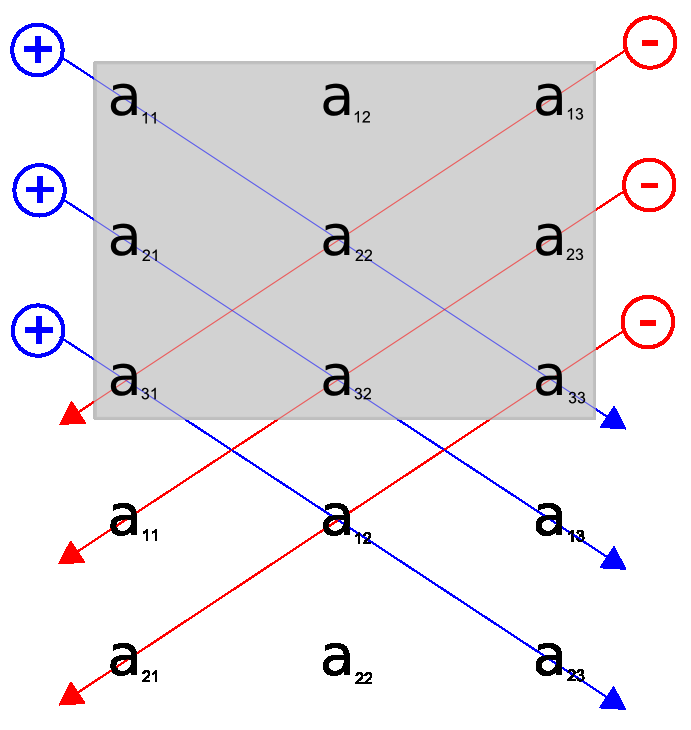
\includegraphics[width=5cm]{matematika/obrazky/sarrusovo_pravidlo.png} \end{center}
\end{poznamka}

\begin{poznamka}
Obecný vzorec lze také vyjádřit pomocí Levi-Civitova symbolu $\epsilon_{{j_1}{j_2}\dots{j_n}}$ jako
$$\det A = \sum_{{j_1},{j_2}, \dots ,{j_n}}\epsilon_{{j_1}{j_2} \dots {j_n}} a_{1,j_1}a_{2,j_2}  \dots  a_{n,j_n} = \sum_{{j_1},{j_2}, \dots ,{j_n}}\epsilon_{{j_1}{j_2} \dots {j_n}} a_{j_1,1}a_{j_2,2}  \dots  a_{j_n,n}$$
\end{poznamka}

\subsubsection*{Vlastnosti determinantu}

\begin{vetaN}{O determinantu transponované matice}
Pro čtvercovou matici $A$ řádu $n$ platí:
$$\det A=\det A^T$$

\begin{dukaz}
Plyne z faktu že $\sgn(p)=\sgn(p^{-1})$:
\begin{align*}
\det(A^T) & =\sum_{p\in S_n}\sgn(p)\prod_{i=1}^n(A^T)_{i,p(i)}=\\
 & =\sum_{p\in S_n}\sgn(p)\prod_{i=1}^n a_{p(i),i}=\sum_{p^{-1}\in S_n}\sgn(p^{-1})\prod_{i=1}^n a_{i,p^{-1}(i)}=\det(A)
\end{align*}
\end{dukaz}
\end{vetaN}

\begin{vetaN}{Přerovnání matice}
Přerovnání řádků nebo sloupců podle permutace $p$ nezmění determinant vůbec, pokud $\sgn(p)=1$ a změní jen jeho znaménko, pokud $\sgn(p)=-1$.

\begin{dukaz}
A buď původní matice a B přerovnaná:
\begin{align*}
\det(B) & =\sum_{p\in S_n}\sgn(p)\prod_{i=1}^n(B)_{i,p(i)} = \sum_{p\in S_n}\sgn(p)\prod_{i=1}^n(A)_{i,q^{-1}\left(p(i)\right)}=\\
 & =\sgn(q)\sum_{p\in S_n}\sgn(q)\sgn(p)\prod_{i=1}^n(A)_{i,q^{-1}\left(p(i)\right)}=\sgn(q)\sum_{p\in S_n}\sgn(h)\prod_{i=1}^n(A)_{i,h(i)}=\\
 & =\sgn(q)\det(A)
\end{align*}
\end{dukaz}
\end{vetaN}

\begin{dusledek}
Má-li matice dva shodné sloupce nebo řádky, má automaticky nulový determinant (přehozením právě těch dvou řádků nebo sloupců vzniknou shodné matice se stejným determinantem, ale má se změnit znaménko).
\end{dusledek}

\begin{vetaN}{Determinant jako lineární funkce}
Determinant matice $A$ je lineární funkcí každého jejího řádku i každého sloupce, tj. platí
\begin{penumerate}
    \item $$\det\left(\begin{matrix}
a_{1,1}& \dots & a_{1,n}\\
\vdots & & \vdots \\
b_{i,1}& \dots & b_{i,n}\\
\vdots & & \vdots \\
a_{n,1}& \dots & a_{n,n}\\
\end{matrix}\right)
+ \det\left(\begin{matrix}
a_{1,1}& \dots & a_{1,n}\\
\vdots & & \vdots \\
c_{i,1}& \dots & c_{i,n}\\
\vdots & & \vdots \\
a_{n,1}& \dots & a_{n,n}\\
\end{matrix}\right)
= \det\left(\begin{matrix}
a_{1,1}& \dots & a_{1,n}\\
\vdots & & \vdots \\
b_{i,1} + c_{i,1}& \dots & b_{i,n} + c_{i,n}\\
\vdots & & \vdots \\
a_{n,1}& \dots & a_{n,n}\\
\end{matrix}\right)$$
    \item $$\det\left(\begin{matrix}
a_{1,1}& \dots & a_{1,n}\\
\vdots & & \vdots \\
\kappa a_{i,n}& \dots & \kappa a_{i,n}\\
\vdots & & \vdots \\
a_{n,1}& \dots & a_{n,n}\\
\end{matrix}\right)
= \kappa \det(A)$$
\end{penumerate}

\begin{dukaz}
První část plyne z distributivity sčítání vzhledem k násobení -- každý člen sumy (produkt prvků) obsahuje jeden prvek typu $b_{i,p(i)} + c_{i,p(i)}$ pro nějakou permutaci a ten je možné rozepsat. Druhá část se dokáže podobně díky komutativitě násobení -- prvek $\kappa$ je také obsažen v každém členu sumy právě jednou, takže je ho možné \uv{vytknout}.
\end{dukaz}
\end{vetaN}

\begin{vetaN}{Determinant součinu matic}
Nechť $A$ a $B$ jsou čtvercové matice stejného řádu $n$ nad tělesem $T$. Potom platí:
$$\det(A\cdot B)=\det(A)\cdot\det(B)$$

\begin{dukaz}
Je-li jedna z matic singulární, je jejich součin singulární a tedy má nulový determinant; stejně jako je nulový součin determinantů původních matic. Jsou-li obě matice regulární, lze $A$ rozložit na nějaký součin $E_1\cdot E_2\cdot\dots\cdot E_k$ elementárních matic. Potom 
\begin{align*}
\det(AB) & = \det(E_1E_2\dots E_k B)=\det(E_1)\cdot\det(E_2\dots E_k B)\\
& =\det(E_1)\det(E_2)\dots\det(E_k)\det(B)=\det(A)\det(B)
\end{align*}
protože víme, jakým způsobem elementární úpravy (ekvivalent elementárních matic ve vzorci) mění determinant.
\end{dukaz}
\end{vetaN}

\begin{dusledek}
Čtvercová matice je regulární, právě když má nenulový determinant.
\end{dusledek}

\subsection{Úpravy determinantů, výpočet}

\begin{obecne}{Gaussova eliminace}
Gaussova metoda spočívá v provedení takových úprav matice, které nemění hodnotu determinantu, ale zjednoduší výpočet jeho hodnoty. Cílem prováděných úprav je získat trojúhelníkovou matici \textbf{A} (kde pro $i > j$ je $a_{i,j} = 0$), neboť pro trojúhelníkové matice platí

$$\det A = a_{1,1} a_{2,2}  \dots  a_{n,n}$$

\noindent
tzn. determinant je roven součinu prvků hlavní diagonály matice.

\noindent
Při úpravách matice pro výpočet determinantu postupujeme podle těchto pravidel:
\begin{pitemize}
\item Pokud \textbf{B} vznikne z \textbf{A} výměnnou dvou řádku nebo sloupců potom $\det B = -\det A$
\item Pokud \textbf{B} vznikne z \textbf{A} vynásobením řádku nebo sloupce skalárem c, potom $\det B = c.\det A$
\item Pokud \textbf{B} vznikne z \textbf{A} přičtením násobku jednoho řádku k jinému, nebo přidáním násobku sloupce k jinému sloupci potom $\det B = \det A$
\end{pitemize}

\noindent
Opakovaným použitím uvedených pravidel převedeme matici na trojúhelníkovou a pro tu poté snadno spočteme determinant.
\end{obecne}



\subsection{Geometrický smysl determinantu}

\begin{obecne}{Matice řádu 2}
Absolutní hodnotu determinantu matice řádu 2
$$\det\left(
\begin{array}{cc}
a & b\\
c & d
\end{array}
\right) = ad - bc
$$
lze interpretovat jako obsah rovnoběžníku s vrcholy v bodech $(0,0)$, $(a,c)$, $(b, d)$ a $(a+b, c+d)$. Znaménko determinantu určuje vzájemnou orientaci vektorů $(a,c)$, $(b, d)$. $\det A$ je kladný, pokud úhel mezi vektory $(a,c)$, $(b, d)$ měřený v kladném směru (tedy proti směru hodinových ručiček) menší než $\pi$, a záporný, pokud je tento úhel větší než $\pi$.
\end{obecne}

\begin{obecne}{Matice řádu 3}
Podobný geometrický význam jako pro matici řádu 2 najdeme i pro matice $B = (b_{i,j})$ řádu 3. Řádkové vektory

$$b_1 = (b_{1,1}, b_{1,2}, b_{1,3}), b_2 = (b_{2,1}, b_{2,2}, b_{2,3}), b_3 = (b_{3,1}, b_{3,2}, b_{3,3})$$

určují v třídimenzionálním prostoru rovnoběžnostěn, jehož objem je roven $\left| \det B \right|$. Pokud je $\det B$ kladný, tak je posloupnost vektorů $b_1, b_2, b_3$ pravotočivá, a levotočivá, pokud je $\det B$ záporný.
\end{obecne}

\begin{obecne}{Matice vyšších řádů}
I v reálných prostorech vyšších řádů lze determinant chápat jako objem obecného \emph{n}-rozměrného rovnoběžnostěnu, případně jako pravotočivost, respektive levotočivost posloupnosti $b_1, b_2,  \dots , b_n$.
\end{obecne}

\begin{definiceN}{Pravotočivá a levotočivá soustava prostorových kartézských souřadnic}
Představte si, že v místě, kde stojíte, je počátek prostorové kartézské soustavy. Osa x nechť směřuje přímo vpřed (směrem, kterým se díváte), osa y nechť směřuje vlevo a osa z nechť směřuje vzhůru. Taková soustava se nazývá \emph{pravotočivá souřadná soustava}.

Zaměníme-li osy x a y, získáme \emph{souřadnou soustavu levotočivou}. Obvykle se pracuje s pravotočivou souřadnou soustavou.

Mnemotechnická pomůcka: Soustava souřadnic je pravotočivá pokud při naznačení kladného směru osy z zdviženým palcem pravé ruky naznačují ostatní prsty směr od kladného směru osy x ke kladnému směru osy y.
\end{definiceN}


\subsection{Minory a inversní matice}

\begin{definiceN}{Minor}
Mějme čtvercovou matici $A_{ij}$, kterou získáme z matice $A$ odstraněním i-tého řádku a j-tého sloupce. Determinant matice $A_{ij}$, tzn. $\det A_{ij}$ nazýváme \emph{subdeterminantem} (též \emph{minorem}) příslušným k prvku $a_{i,j}$ matice $A$.
\end{definiceN}

\begin{obecne}{Výpočet determinantu rozvojem podle řádků (sloupců)}
Algebraický doplněk lze použít k výpočtu determinantu \emph{n}-tého řádu. Pro libovolné (pevně dané) \emph{i} lze determinant matice $A$ vyjádřit pomocí algebraických doplňků jako

$$\det( A ) = \sum_{j=1}^n a_{i,j}\cdot (-1)^{i+j}\det( A_{ij} )$$

Tento postup je označován jako \emph{rozvoj (rozklad) determinantu podle i-tého řádku}. Ekvivalentně lze determinant vyjádřit \emph{rozvojem (rozkladem) podle j-tého sloupce}. Číslo $(-1)^{i+j}\det( A_{ij} )$ se někdy nazývá \emph{kofaktorem} nebo \emph{algebraickým doplňkem}.
\end{obecne}

\begin{definiceN}{Adjungovaná matice}
Pro čtvercovou matici $A$ definujeme \emph{adjungovanou matici} $\adj A$ předpisem
$$(\adj A)_{i,j}=(-1)^{i+j}\cdot\det(A_{ji})$$
kde $A_{ji}$ jsou minory matice $A$ (s vynechaným $j$-tým řádkem a $i$-tým sloupcem -- pozor na obrácené pořadí indexů!). Prvky adjungované matice jsou vlastně algebraické doplňky v transponované matici $A^T$.
\end{definiceN}

\begin{definiceN}{Inversní matice}
Pro čtvercovou matici $A$ řádu $n$ definujeme inverzní matici $A^{-1}$ předpisem
$$A.A^{-1} = A^{-1}.A = I_n$$
kde $I_n$ je jednotková matice. Inversní matici lze sestrojit pouze pro regulární matici.
\end{definiceN}

\begin{vetaN}{Výpočet inversní matice podle minorů}
Pro každou regulární matici $A$ nad tělesem $T$ platí: 
$$A^{-1}=\frac{1}{\det A}\cdot(\adj A)$$
$$A^{-1}_{i,j}=(-1)^{i+j}\frac{\det(A_{ji})}{\det A}$$

\begin{dukaz}
Z maticového součinu $A\cdot\adj A$:
\begin{penumerate}
    \item $i$-tý řádek $A$ $\times$ $i$-tý sloupec $\adj A$ (obs. determinanty minorů odp. $i$-tému řádku) dá dohromady $\det A$
    (z rozvoje determinantu podle řádku)
    \item $j$-tý řádek $A$ $\times$ $i$-tý sloupec $\adj A$ dá dohromady $0$, protože jde o stejný princip pro matici, kde $i$-tý
    řádek je nahrazen $j$-tým (2 stejné řádky)
\end{penumerate}
Potom $A\cdot\adj A = \det A\cdot I_n$ a to už dává $\frac{1}{\det A}\adj A = A^{-1}$.
\end{dukaz}
\end{vetaN}


\subsection{Cramerovo pravidlo}
Cramerovo pravidlo je metoda umožňující nalezení řešení soustavy lineárních algebraických rovnic.

\begin{obecne}{Postup}
Mějme soustavu lineárních rovnic, která obsahuje stejný počet neznámých jako je počet rovnic. Označme matici soustavy $A$. Dále označme $A_i\;$ jako matici, kterou získáme z matice $A$, nahradíme-li v ní $i$-tý sloupec sloupcem pravých stran soustavy rovnic.

Pokud zapíšeme matice soustavy a vektor pravých stran jako

$$
A =
\left( \begin{array}{cccc}
    a_{11} & a_{12} & \dots  & a_{1n} \\
	a_{21} & a_{22} &  \dots  & a_{2n} \\
	\vdots  &  \vdots  &  \ddots  &  \vdots \\
	a_{m1} & a_{m2} &  \dots  & a_{mn}
\end{array} \right), 
B = \left( \begin{array}{cccc} b_1 \\b_2 \\ \vdots  \\b_m \end{array} \right)
$$

pak má tvar

$$
A_i=
\left( \begin{array}{cccccccc}
	a_{11} & a_{12} & \dots & a_{1,i-1} & b_1 & a_{1,i+1} & \dots  & a_{1n} \\
	a_{21} & a_{22} & \dots & a_{2,i-1} & b_2 & a_{2,i+1} & \dots  & a_{2n} \\
	\vdots & \vdots & \vdots & \vdots & \vdots & \vdots & \ddots & \vdots \\
	a_{m1} & a_{m2} & \dots & a_{m,i-1} & b_m & a_{m,i+1} & \dots & a_{mn}
\end{array} \right)
$$

Pokud je determinant matice soustavy nenulový, $\det A \neq 0$, tzn. matice je regulární, pak má soustava právě jedno řešení, pro které platí

$$x_i = \frac{\det A_i}{\det A}$$

pro $i = 1,2, \dots ,n$.
\end{obecne}

\begin{dukaz}
Pro soustavu $Ax=b$ -- rozepíšeme $x=A^{-1}b$, ze vzorce pro inversní matici plyne
$$x=\frac{1}{\det A}(\adj A)\cdot b$$
takže pro $x_i$ vychází 
$$x_i=\frac{1}{\det A}((\adj A)b)_i=\frac{1}{\det A}\cdot\sum_{j=1}^n(\adj A)_{i,j}\cdot b_j=\frac{1}{\det A}\cdot\det A_i$$
\end{dukaz}

\begin{priklad}
Úkolem je řešit soustavu rovnic
 $$x + y = 3$$
 $$x - 2y = 1$$

Determinant matice soustavy je
 $$\det A = \left| \begin{array}{cc}1 & 1 \\ 1 & -2\end{array} \right| = -3$$

Poněvadž je $\det A \neq 0$, lze použít Cramerovo pravidlo.

Dále určíme
 $$\det A_1 = \left| \begin{array}{cc}3 & 1 \\ 1 & -2\end{array} \right| = -7$$
 $$\det A_2 = \left| \begin{array}{cc}1 & 3 \\ 1 & 1\end{array} \right| = -2$$

Řešení má tedy tvar
 $$x = \frac{\det A_1}{\det A} = \frac{-7}{-3} = \frac{7}{3}$$
 $$y = \frac{\det A_2}{\det A} = \frac{-2}{-3} = \frac{2}{3}$$

Zkouškou se přesvědčíme, že se skutečně jedná o řešení uvedené soustavy.
\end{priklad}

\newpage
\section{Vlastní čísla a vlastní hodnoty}


\begin{pozadavky}
\begin{pitemize}
\item Vlastní čísla a vlastní hodnoty lineárního operátoru resp. čtvercové matice.
\item Jejich výpočet.
\item Základní vlastnosti.
\item Uvedení matice na diagonální tvar.
\item Informace o Jordanově tvaru v obecném případě.
\end{pitemize}
\end{pozadavky}

Otázka vychází především ze skript pana Jiřího Tůmy a částečně i ze skript pana Jiřího Rohna.

\subsection{Definice}
\begin{definice}
Nechť \textbf{A} je čtvercová matice řádu n s reálnými (komplexními) prvky. Jestliže platí
\begin{equation}\label{1}Ax = \lambda x\end{equation}
pro jisté $\lambda \in \mathbb{C}$ a pro \emph{nenulový vektor} $x \in \mathbb{R}^{n\times1}\ (\mathbb{C}^{n\times1}) $. Pak $\lambda$ nazveme \emph{vlastním číslem} matice
\textbf{A} a vektor x \emph{vlastním vektorem} příslušným k tomuto vlastnímu číslu.

Množinu všech vlastních čísel matice \textbf{A} nazýváme \emph{spektrum} matice \textbf{A} a označujeme ji $\sigma$(\textbf{A}).

Funkci $p(\lambda) = \det(\textbf{A} - \lambda \textbf{I}_n)$ nazveme \emph{charakteristický polynom} matice \textbf{A}.
\end{definice}

\begin{pozorovani}
Z definice přímo plyne:

$$\lambda \in \sigma(\textbf{A}) \Leftrightarrow \quad\textit{matice}\quad \textbf{A} - \lambda \textbf{I}_n \quad\textit{je\quad singulární}\quad \Leftrightarrow \det( \textbf{A} - \lambda \textbf{I}_n ) = 0$$

Poslední podmínka nám říká, jak najít vlastní čísla matice, pokud existují.
Vlastní vektory vypočteme úpravou (\ref{1}) na: \begin{displaymath}(\textbf{A}-\lambda \textbf{I}_n)x=0\end{displaymath}
\end{pozorovani}

\begin{definice}
Je-li $F:\textbf{V}\rightarrow$\textbf{V} lineární operátor na reálném (komplexním) vektorovém prostoru \textbf{V}, pak skalár $\lambda$ nazýváme \emph{vlastní číslo} lineárního operátoru \textbf{V}, pokud existuje nenulový vektor $x \in \textbf{V}$, pro který platí $F(x)=\lambda x$.
Je-li $\lambda$ vlastní číslo operátoru F, pak každý vektor $x \in \textbf{V}$, pro který platí $F(x)=\lambda x$, nazýváme \emph{vlastní vektor} lineárního operátoru $F$ příslušný vlastnímu číslu $\lambda$.
Množinu všech vlastních čísel operátoru $F$ označujeme $\sigma(F)$ a nazýváme \emph{spektrum} operátoru $F$.
\end{definice}

\begin{definiceN}{podobné matice, diagonalizovatelnost}
Řekneme, že matice \textbf{A} a \textbf{B} jsou \emph{podobné}, pokud existuje nějaká regulární matice \textbf{P} taková, že platí $\textbf{B}=\textbf{P}^{-1}\textbf{A}\textbf{P}$.

Reálná(komplexní) matice \textbf{A} řádu n  se nazývá \emph{diagonalizovatelná}, pokud existuje regulární reálná(komplexní) matice \textbf{P} řádu $n$, pro kterou platí, že součin $\textbf{P}^{-1}\textbf{A}\textbf{P}$ je diagonální matice, tj. pokud matice \textbf{A} je podobná nějaké diagonální matici.

Lineární operátor $F:\textbf{V}\rightarrow$\textbf{V} na reálném(komplexním) vektorovém prostoru \textbf{V} se nazývá \emph{diagonalizovatelný}, pokud existuje báze $\mathbb{B}$ prostoru \textbf{V}, pro kterou platí, že matice $[F]_B$ operátoru $F$ vzhledem k bázi $\mathbb{B}$ je diagonální.
\end{definiceN}

\subsection{Výpočet vlastních čísel a vlastních vektorů }

\begin{priklad}

$$\mathbf{A} =
\begin{pmatrix}
  3 & 2 \\
  2 & 6 \\
\end{pmatrix}\text{, spočítáme tedy kdy se } \det
\begin{pmatrix}
  3-\lambda & 2 \\
  2 & 6-\lambda \\
\end{pmatrix} = 0$$

$$\det\begin{pmatrix}
  3-\lambda & 2 \\
  2 & 6-\lambda \\
\end{pmatrix} = (3-\lambda)(6-\lambda)-4 = \lambda^2 - 9\lambda + 14$$

$$\lambda^2 - 9\lambda + 14 = 0 \quad \text{dává dvě řešení:} \quad \lambda_1 = 2 \text{ a } \lambda_2 = 7$$

\noindent vlastní vektor příslušný vlastnímu číslu $\lambda_1 = 2$:

$$\begin{pmatrix}
  3 & 2 \\
  2 & 6 \\
\end{pmatrix} -
\begin{pmatrix}
  2 & 0 \\
  0 & 2 \\
\end{pmatrix} =
\begin{pmatrix}
  1 & 2 \\
  2 & 4 \\
\end{pmatrix}$$

$$\begin{pmatrix}
  1 & 2 \\
  2 & 4 \\
\end{pmatrix}x = 0 \Rightarrow x=(-2,1)$$

\noindent vlastní vektor příslušný vlastnímu číslu $\lambda_2 = 7$:

$$\begin{pmatrix}
  3 & 2 \\
  2 & 6 \\
\end{pmatrix} -
\begin{pmatrix}
  7 & 0 \\
  0 & 7 \\
\end{pmatrix} =
\begin{pmatrix}
  -4 & 2 \\
  2 & -1 \\
\end{pmatrix}$$

$$\begin{pmatrix}
  -4 & 2 \\
  2 & -1 \\
\end{pmatrix}x = 0 \Rightarrow x=(1,2)$$
\end{priklad}

\subsection{Vlastnosti}

\begin{vetaN}{vlastnosti vlastních čísel}
Pro komplexní čtvercovou matici \textbf{A} řádu $n$ platí:
\begin{penumerate}
  \item charakteristický polynom matice \textbf{A} řádu $n$ je polynom stupně $n$ s vedoucím koeficientem rovným $(-1)^n$
  \item komplexní číslo $\lambda$ je vlastním číslem matice \textbf{A} právě když je kořenem charakteristického polynomu $p(\lambda)$ matice \textbf{A}
  \item matice \textbf{A} má $n$ vlastních komplexních čísel, počítáme-li každé tolikrát, kolik je jeho násobnost jako kořene charakteristického polynomu
  \item pokud \textbf{A} je reálná matice, pak $\lambda \in \sigma(\textbf{A})$ právě když komplexně sdružené $\overline{\lambda} \in \sigma(\textbf{A})$
\end{penumerate}

\medskip
\begin{dukaz}
\begin{penumerate}
    \item plyne z definice determinantu.
    \item $\exists x\neq 0: \mathbf{A}x=\lambda x\ \Leftrightarrow\ \mathbf{A}x-\lambda x=0\ \Leftrightarrow\ (\mathbf{A}-\lambda \textbf{I}_n)x=0$, tj. matice $(\mathbf{A}-\lambda \textbf{I}_n)$ je singulární, takže musí mít nulový determinant.
    \item plyne ze Základní věty algebry.
    \item taktéž.
\end{penumerate}
\end{dukaz}
\end{vetaN}

\begin{veta}
Determinant čtvercové matice je roven součinu jejích vlastních čísel.
\end{veta}

\begin{veta}
Vlastními čísly horní(dolní) trojúhelníkové matice jsou právě všechny diagonální prvky.
\end{veta}

\begin{veta}
Je-li \textbf{A} reálná symetrická matice, pak každé vlastní číslo matice \textbf{A} je reálné.
\end{veta}

\begin{veta}
Je-li \textbf{A} čtvercová reálná(komplexní) matice řádu n, \textbf{P} reálná(komplexní) regulární matice stejného řádu a $\textbf{B}=\textbf{P}^{-1}\textbf{A}\textbf{P}$, pak obě matice \textbf{A} a \textbf{B} mají stejný charakterictický polynom a tedy i stejné spektrum.

\medskip
\begin{dukaz}
$\det(\textbf{P}^{-1}\textbf{AP}-t\textbf{I})=\det(\textbf{P}^{-1}\textbf{AP}-t\textbf{P}^{-1}\textbf{IP})=\det(\textbf{P}^{-1})\cdot\det(\mathbf{A}-t\mathbf{I})\cdot{\det(\mathbf{P}})=\det(\mathbf{A}-t\mathbf{I})$.
\end{dukaz}
\end{veta}

\begin{veta}
Jsou-li \textbf{A}, \textbf{B} čtvercové matice stejného typu, potom \textbf{AB} a \textbf{BA} mají stejná vlastní čísla.
\end{veta}

\subsection{Uvedení matice na diagonální tvar}

\begin{vetaN}{O diagonalizovatelnosti a bázi}
Čtvercová reálná(komplexní) matice \textbf{A} řádu $n$ je diagonalizovatelná, právě když existuje báze prostoru \ $\mathbb{R}^n\ (\mathbb{C}^n)$, která je složena z vlastních vektorů matice \textbf{A}.

Lineární operátor $F:\textbf{V}\rightarrow$\textbf{V} na reálném(komplexním) vektorovém prostoru \textbf{V} je diagonalizovatelný právě když existuje báze prostoru \textbf{V} složená z vlastních vektorů operátoru $F$.

\medskip
\begin{dukaz}
Je-li \textbf{A} diagonalizovatelná, znamená to, že existuje regulární matice \textbf{R} taková, že $\textbf{R}^{-1}\textbf{AR} = \textbf{D}$ (a \textbf{D} je diagonální), což je to samé jako $\textbf{AR} = \textbf{RD}$. Sloupce matice R tvoří vlastní vektory příslušné vlastním číslům matice \textbf{A}. \textbf{R} je regulární, takže vlastní vektory jsou lineárně nezávislé a tedy tvoří bázi.

Mám-li $n$ lineárně nezávislých vlastních vektorů, mohu z nich sestavit matici \textbf{R} a pro ní už platí, že $\textbf{R}^{-1}\textbf{AR} = \textbf{D}$.
\end{dukaz}
\end{vetaN}

\begin{dusledek}
Je-li \textbf{A} čtvercová matice řádu n a \textbf{P} regulární matice taková, že $\textbf{P}^{-1}\textbf{A}\textbf{P}=\textbf{D}$ pro nějakou diagonální matici \textbf{D}, pak na hlavní diagonále matice \textbf{D} jsou všechna vlastní čísla matice \textbf{A}.
\end{dusledek}

\begin{vetaN}{Vlastní čísla a diagonalizovatelnost}
Platí:
\begin{penumerate}
    \item Jsou-li $\lambda_1,...,\lambda_m$ navzájem různá vlastní čísla matice \textbf{A} řádu $n$ a $u_i\neq0$ je vlastní vektor matice \textbf{A} příslušný vlastnímu číslu $\lambda_i$ pro libovolné $i=1,...,m$, pak je posloupnost vektorů $u_1,\dots,u_m$ lineárně nezávislá.

    \item Má-li matice \textbf{A} řádu $n$ celkem $n$ navzájem různých vlastních čísel, pak je diagonalizovatelná.

    \item Má-li lineární operátor $F:\textbf{V}\rightarrow\textbf{V}$ celkem $n$ navzájem různých vlastních čísel, pak je diagonalizovatelný.
\end{penumerate}

\medskip
\begin{dukaz}
\begin{penumerate}
    \item indukcí a sporem, $u_1,\dots,u_k$ dávají nejmenší protipříklad, pak z rovnice $0=\mathbf{A}0=\sum_{i=1}^k a_i\lambda_iu_i$ a $0=\lambda_k\cdot 0=\lambda_k\cdot\sum_{i=1}^k a_i u_i$, pak dostávám spor (buď byly $u_1,\dots,u_{k-1}$ závislé, nebo je $u_k$ nulové)
    \item z $n$ lineárně nezávislých vlastních vektorů sestrojím matici \textbf{R} a platí \textbf{AR}=\textbf{RD}, kde \textbf{D} je diagonální matice s vlastními čísly na diagonále.
\end{penumerate}
\end{dukaz}
\end{vetaN}

\begin{vetaN}{O diagonalizovatelnosti a násobnostech}
Čtvercová reálná(komplexní) matice \textbf{A} řádu $n$ je diagonalizovatelná, právě když pro každé vlastní číslo $\lambda$ matice \textbf{A} platí, že algebraická násobnost $\lambda$ se rovná dimenzi nulového prostoru matice $\textbf{A}-\lambda \textbf{I}_n$ , tj. číslu $\dim \mathcal{N}(\textbf{A}-\lambda \textbf{I}_n)$.

Neboli: čtvercová matice \textbf{A} řádu $n$ je diagonalizovatelná, právě když pro každé její vlastní číslo $\lambda_i$ s násobností $r_i$ platí $\mathrm{rank}(\mathbf{A}-\lambda_i I)=n-r_i$.

\medskip
\begin{dukaz}
Matice je diagonalizovatelná, právě když existuje báze prostoru $\mathbb{C}^n$ ($\mathbb{R}^n$), složená z vlastních vektorů, a tu lze rozložit na $k$ bází $\mathrm{Ker}(\textbf{A}-\lambda\textbf{I})$, které mají dimenzi $r_i$.
\end{dukaz}
\end{vetaN}

\begin{vetaN}{spektrální věta pro diagonalizovatelné matice}
Čtvercová matice \textbf{A} řádu n se spektrem $\sigma(\textbf{A}) = \{\lambda_1,...,\lambda_t\}$ je diagonalizovatelná právě když existují matice $\textbf{E}_1,...,\textbf{E}_t$ řádu n, pro které platí:
\begin{penumerate}
  \item $\textbf{A} = \lambda_1 \textbf{E}_1 + \lambda_2 \textbf{E}_2 + ... + \lambda_t \textbf{E}_t$
  \item ${\textbf{E}_i}^2 = \textbf{E}_i$ pro každé $i = 1,2,...,t$
  \item $\textbf{E}_i \textbf{E}_j = 0$ pro libovolné dva různé indexy $i,j = 1,2,...,t$
  \item $\textbf{E}_1 + \textbf{E}_2 + ... + \textbf{E}_t = \textbf{I}_n$

  \bigskip
  Dále pro diagonalizovatelnou matici \textbf{A} platí, že
  \item matice $\textbf{E}_i$ jsou jednoznačně určené maticí \textbf{A} a vlastnostmi \textit{1,2,3,4}
  \item hodnost každé z matic $\textbf{E}_i$ se rovná algebraické násobnosti vlastního čísla $\lambda_i$
  \item je-li $f(x)= c_0 + c_1 x + ... + c_k x^k$ libovolný polynom s komplexními koeficienty, pak platí $f(\textbf{A})= c_0 \textbf{I}_n + c_1 \textbf{A} + ... + c_k \textbf{A}^k = f(\lambda_1)\textbf{E}_1 + f(\lambda_2)\textbf{E}_2 + ... + f(\lambda_k)\textbf{E}_k$
  \item nějaká matice \textbf{B} komutuje s maticí \textbf{A} (tj. $\textbf{AB}=\textbf{BA}$) právě tehdy, když komutuje s každou z matic $\textbf{E}_i$ pro $i = 1,2,...,t$
\end{penumerate}
\end{vetaN}

\subsection{Jordanův tvar v obecném případě }
\begin{definiceN}{Jordanův tvar}
Diagonalizovatelné matice mají dobře pochopitelnou strukturu popsanou ve spektrální větě. Matice, které nelze diagonalizovat, nemají bázi složenou z vlastních vektorů, musí mít nějaké vícenásobné vlastní číslo $\lambda$, pro které je dimenze nulového prostoru $\mathcal{N}(\textbf{J}-\lambda \textbf{I}_n)$ menší než algebraická násobnost čísla $\lambda$. (viz věta o diagonalizovatelnosti a násobnostech)

Příklad takové matice řádu $n$, pro $n\geq2$

$$\textbf{J} = \begin{pmatrix}
  \lambda & 1 & 0 & 0 & \cdots & 0 & 0 \\
  0 & \lambda & 1 & 0 & \cdots & 0 & 0 \\
  0 & 0 & \lambda & 1 & \cdots & 0 & 0 \\
  0 & 0 & 0 & \lambda & \cdots & 0 & 0 \\
   &  & \vdots &  & \ddots &  & \vdots \\
  0 & 0 & 0 & 0 & \cdots & \lambda & 1 \\
  0 & 0 & 0 & 0 & \cdots & 0 & \lambda \\
\end{pmatrix}$$

Všechny prvky na diagonále se rovnají stejnému číslu $\lambda$, všechny prvky bezprostředně nad hlavní diagonálou  se rovnají 1, ostatní prvky jsou nulové.
\end{definiceN}
\begin{pozorovani}
Charakteristický polynom matice \textbf{J} se rovná:
$$p(t)=(\lambda - t)^n$$
\end{pozorovani}

\begin{pozorovani}
Matice $\textbf{J}-\lambda \textbf{I}_n$ je v řádkově odsťupňovaném tvaru, její hodnost se rovná $n-1$ a její nulový prostor $\mathcal{N}(\textbf{J}-\lambda \textbf{I}_n)$ má proto dimenzi rovnou 1, což se nerovná algebraické násobnosti vlastního čísla $\lambda$, matice \textbf{J} tedy není diagonalizovatelná.
\end{pozorovani}

\begin{definiceN}{Jordanova buňka}
Matice \textbf{J} se nazývá Jordanova buňka řádu $n$ příslušná vlastnímu číslu $\lambda$.
\end{definiceN}

\begin{vetaN}{O Jordanově kanonickém tvaru}
Pro každou čtvercovou matici \textbf{A} existuje regulární matice \textbf{P} taková, že

$$\textbf{P}^{-1}\textbf{A}\textbf{P} = \begin{pmatrix}
  \textbf{J}_1 & 0 & 0 & \cdots & 0 \\
  0 & \textbf{J}_2 & 0 & \cdots & 0 \\
  0 & 0 & \textbf{J}_3 & \cdots & 0 \\
   & \vdots &  & \ddots & \vdots \\
  0 & 0 & 0 & \cdots & \textbf{J}_k \\
\end{pmatrix}$$

kde každá z matic $\textbf{J}_i$ pro $i=1,...,k$ je Jordanova buňka nějakého řádu $n_i$ příslušná vlastnímu číslu $\lambda_i$. Čísla $\lambda_1,...,\lambda_k$ jsou všechna, nikoliv nutně různá, vlastní čísla matice \textbf{A} a platí dále $n_1 + ... + n_k = n$. Dvojice $n_i,\lambda_i$ pro $i=1,...,k$ jsou maticí \textbf{A} určené jednoznačně až na pořadí (tj. reprezentují třídu podobných matic).
\end{vetaN}


\begin{definiceN}{Hermitovskost}
Nechť \textbf{A} je komplexní matice, potom matici $\textbf{A}^H$, pro kterou platí, že $(\textbf{A}^H)_{ij} = \overline{a_{ji}}$ nazýváme 
\emph{hermitovskou transpozicí} matice \textbf{A} (někdy se používá název \uv{konjugovaná matice}). 

Komplexní čtvercová matice \textbf{A} se nazývá \emph{unitární}, pokud platí, že $\textbf{A}^H\textbf{A} = \textbf{I}$. 
Komplexní čtvercová matice \textbf{A} se nazývá \emph{hermitovská}, pokud $\textbf{A}^H = \textbf{A}$.
\end{definiceN}

\begin{pozorovani}
Platí: $(\textbf{AB})^H = \textbf{B}^H\textbf{A}^H$ (důkaz je stejný jako pro obyčejnou transpozici). 
\end{pozorovani}

\def\Complex{\mathbb{C}}
\def\Real{\mathbb{R}}

\begin{vetaN}{O hermitovských maticích} 
Každá hermitovská matice $A$ má všechna vlastní čísla reálná ( i když je sama komplexní). Navíc existuje unitární matice $R$ taková, že $R^{-1}A R$ je diagonální. (tzn. hermitovská matice je diagonalizovatelná).
\end{vetaN}

\begin{dusledek} Interpretace v $\Real$:
Pro každou symetrickou matici $A$ platí, že všechna její vl. čísla jsou reálná a navíc existuje ortogonální matice $R$: $R^{-1}AR$ je diagonální.
Příslušný vl. vektor $x$ lze vzít reálný, protože $(A - \lambda I)x = 0$ -- soustava lin. rovnic s reálnou singulární maticí -- musí mít netriviální reálné řešení.
\end{dusledek}


\subsection{Spektrální věta - část důkazu}

\ramcek{10cm}{Tato část není v požadavcích ke zkouškám!}

\begin{dukaz}
Důkaz spektrální věty je poměrně dlouhý - několik stránek, uvedu zde tedy jen část důkazu, doufám že tu lehčí :)

\bigskip
\noindent \textbf{\uv{A je diagonalizovatelná $\Rightarrow$  vlastnosti  1,2,3,4}}

Nechť $m_i$ je algebraická násobnost vlastního čísla $\lambda_i$ pro $i=1,...,t$. Matice \textbf{A} je diagonalizovatelná, tedy dle \textbf{Definice 3} existuje regulární matice \textbf{P} řádu n taková, že součin $\textbf{P}^{-1}\textbf{A}\textbf{P}$ je diagonální matice, a tato diagonální matice má na diagonále vlastní čísla matice \textbf{A} dle \textbf{důsledku tvrzení 7 TODO}.  Tedy

\begin{equation}\label{pap}
\textbf{P}^{-1}\textbf{A}\textbf{P} = \begin{pmatrix}
  \lambda_1 \textbf{I}_{m_1} & 0 & \cdots & 0 \\
  0 & \lambda_2 \textbf{I}_{m_2} & \cdots & 0 \\
  \vdots & \vdots & \ddots & \vdots \\
  0 & 0 & \cdots & \lambda_t \textbf{I}_{m_t} \\
\end{pmatrix}
\end{equation}

kde $\textbf{I}_{m_i}$ jsou jednotkové matice řádu $m_i$. Označíme pro $i=1,...,t$ symbolem $\textbf{D}_i$ matici, kterou dostaneme z blokové matice na pravé straně poslední rovnosti tak, že nahradíme všechny výskyty vlastního čísla $\lambda_i$ číslem 1 a výskyty ostatních vlastních čísel $\lambda_j$ pro $j \neq i$ číslem 0. Například

$$\textbf{D}_2 = \begin{pmatrix}
  0 & 0 & \cdots & 0 \\
  0 & \textbf{I}_{m_2} & \cdots & 0 \\
  \vdots & \vdots & \ddots & \vdots \\
  0 & 0 & \cdots & 0 \\
\end{pmatrix}$$

Jedná se vlastně o "částečnou" jednotkovou matici, která má pouze na části diagonály čísla 1. Pak platí:

\begin{equation*}
\begin{split}
\textbf{I}_n & = \textbf{D}_1 + \textbf{D}_2 + ... + \textbf{D}_t\\
\textbf{P}^{-1}\textbf{A}\textbf{P} & = \lambda_1 \textbf{D}_1 + \lambda_2 \textbf{D}_2 + ... + \lambda_t \textbf{D}_t\\
\textbf{A} & = \lambda_1\textbf{P}\textbf{D}_1\textbf{P}^{-1} + \lambda_2\textbf{P}\textbf{D}_2\textbf{P}^{-1} + ... + \lambda_t\textbf{P}\textbf{D}_t\textbf{P}^{-1}
\end{split}
\end{equation*}
V první rovnosti jsme vlastně jen sečetli "částečné jednotkové matice" $\textbf{D}_i$ a výsledek je jednotková matice. Pokud všechny matice $\textbf{D}_i$ vynásobíme vlastními čísly $\lambda_i$ a sečteme je, dostaneme matici na pravé straně rovnice (\ref{pap}). A ve třetí rovnosti se jen zbavíme matic $\textbf{P}$ a $\textbf{P}^{-1}$ na levé straně.

Položíme $\textbf{E}_i = \textbf{P}\textbf{D}_i\textbf{P}^{-1}$ pro $i=1,...,t$ a dostaneme tak z třetí rovnosti vlastnost 1.

Protože ${\textbf{D}_i}^2 = \textbf{D}_i$ a $\textbf{D}_i\textbf{D}_j = 0$ pro libovolné různé indexy $i,j,=1,...,t$ , dostáváme

\begin{equation*}
\begin{split}
{\textbf{E}_i}^2 & = \textbf{P}\textbf{D}_i\textbf{P}^{-1}\textbf{P}\textbf{D}_i\textbf{P}^{-1} = \textbf{P}{\textbf{D}_i}^2\textbf{P}^{-1} = \textbf{P}\textbf{D}_i\textbf{P}^{-1} = \textbf{E}_i\\
\textbf{E}_i\textbf{E}_j & = \textbf{P}\textbf{D}_i\textbf{P}^{-1}\textbf{P}\textbf{D}_j\textbf{P}^{-1} = \textbf{P}\textbf{D}_i\textbf{D}_j\textbf{P}^{-1} = \textbf{P}0\textbf{P}^{-1} = 0\\
\textbf{E}_1 + ... + \textbf{E}_t & = \textbf{P}\textbf{D}_1\textbf{P}^{-1} + ... + \textbf{P}\textbf{D}_t\textbf{P}^{-1} = \textbf{P}(\textbf{D}_1 + ... + \textbf{D}_t)\textbf{P}^{-1} =\\
& = \textbf{P}\textbf{I}_n\textbf{P}^{-1} = \textbf{I}_n
\end{split}
\end{equation*}
což dokazuje vlastnosti 2,3,4.
V první rovnosti jsme využili, že ${\textbf{D}_i}^2 = \textbf{D}_i$ ,  ve druhé jsme využili $\textbf{D}_i\textbf{D}_j = 0$ a ve třetí $\textbf{I}_n = \textbf{D}_1 + \textbf{D}_2 + ... + \textbf{D}_t$.

Opačnou implikaci, tedy že z vlastností 1,2,3,4 plyne diagonalizovatelnost matice nebudu dokazovat. Ze zbývajících vlastností 5,6,7,8 dokážu vlastnosti 6 a 7.

\bigskip
\noindent \textbf{Vlastnost 6}

Matice $\textbf{D}_i$ (z předchozího důkazu), má hodnost $m_i$, proto má tutéž hodnost i matice $\textbf{E}_i = \textbf{P}\textbf{D}_i\textbf{P}^{-1}$ , což dokazuje 6.

\bigskip
\noindent \textbf{Vlastnost 7}

Tento důkaz vypadá na první pohled odporně ale nenechte se odradit :) je to pouze rozepisování sum.

\bigskip
\noindent Dle vlastnosti 1 :
$$\textbf{A}^2 = (\lambda_1\textbf{E}_1 + ... + \lambda_t\textbf{E}_t)(\lambda_1\textbf{E}_1 + ... + \lambda_t\textbf{E}_t)$$

\noindent to se rovná (jen přepsaní na sumu, násobení každý s každým)
$$\sum_{i,j=1}^t \lambda_i \textbf{E}_i \lambda_j \textbf{E}_j$$

\noindent dáme li matice k sobě, vznikne nám $\textbf{E}_i\textbf{E}_j$ což je dle vlastnosti 3 rovno nule (pro různé indexy i a j), tyto násobení tedy můžeme ignorovat a přepsat sumu tak, aby se mezi sebou násobili pouze matice se stejným indexem. Dále víme z vlasnosti 2 že ${\textbf{E}_i}^2 = \textbf{E}_i$ , tedy
$$\sum_{i=1}^t {\lambda_i}^2 {\textbf{E}_i}^2 = \sum_{i=1}^t {\lambda_i}^2 {\textbf{E}_i}$$

\noindent jestliže nyní předpokládáme
$$\textbf{A}^l = \sum_{i=1}^t {\lambda_i}^l {\textbf{E}_i}$$

\noindent pro nějaké $l\geq2$, pak dostáváme (a upravujeme stejně jako v předchozím případě)
\begin{equation*}
\begin{split}
\textbf{A}^{l+1} & = (\lambda_1\textbf{E}_1 + ... + \lambda_t\textbf{E}_t)({\lambda_1}^l{\textbf{E}_1}^l + ... + {\lambda_t}^l{\textbf{E}_t}^l) =\\
& = \sum_{i,j=1}^t \lambda_i \textbf{E}_i {\lambda_j}^l {\textbf{E}_j}^l = \sum_{i=1}^t {\lambda_i}^{l+1} {\textbf{E}_i}^2 = \sum_{i=1}^t {\lambda_i}^{l+1} \textbf{E}_i
\end{split}
\end{equation*}

\noindent Protože rovněž platí
$$\textbf{A}^0 = \textbf{I}_n = \textbf{E}_1 + ... + \textbf{E}_t = {\lambda_1}^0 \textbf{E}_1 + ... + {\lambda_t}^0 \textbf{E}_t$$

\noindent tedy jsme dokázali, že rovnost
$$\textbf{A}^l = \sum_{i=1}^t {\lambda_i}^l {\textbf{E}_i}$$

\noindent platí pro každé nezáporné celé číslo $l$. Pro každé číslo $j = 0,...k$ dostáváme
$$c_j \textbf{A}^j = c_j \sum_{i=1}^t {\lambda_i}^j {\textbf{E}_i}$$

\noindent a tedy platí
$$f(\textbf{A}) = \sum_{j=0}^k c_j{\textbf{A}_j} = \sum_{j=0}^k c_j(\sum_{i=1}^t {\lambda_i}^j {\textbf{E}_i}) = \sum_{i=1}^t (\sum_{j=0}^k c_j {\lambda_i}^j){\textbf{E}_i} = \sum_{i=1}^t f(\lambda_i) \textbf{E}_i$$
\end{dukaz}

\newpage
\section{Základy lineárního programování}

\begin{pozadavky}
\begin{pitemize}
	\item Simplexová metoda
	\item Věty o dualitě (bez důkazu)
\end{pitemize}
\end{pozadavky}

\ramcek{14cm}{Lineární programování je označení pro úlohu maximalizovat jistou funkci $n$ reálných proměnných na množině bodů polytopu v prostoru $\mathbb{R}^n$.}

Nejprve si udělejme malý výlet do geometrie. {\it Polytop} je zobecněním polygonu
(mnohoúhelníku) do vyšších dimenzích. Pro dimenzi $3$ se ale používá ještě speciální
název {\it polyhedron} a pro dimenzi $4$ {\it polychoron}. My se v dalším textu
omezíme na {\it konvexní polytopy}, což jsou konvexní obaly konečně mnoha bodů.
Vzhledem k tomu, že tyto konvexní polytopy jsou průnikem jistého množství poloprostorů,
můžeme je popsat maticovou rovnicí tvaru \[Ax\leq b,\] kde $A$ je matice řádu $m\times n$
a $m$ je počet poloprostorů, jejichž průnikem je daný polytop,
a $n$ je dimenze podprostoru, ve kterém polytop máme.

{\it Simplex} je \uv{$n$--dimenzionální} trojúhelník (průnik několika poloprostorů). Podle rostoucí dimenze je to tedy po řadě bod, úsečka, trojúhelník, čtyřstěn, pentachoron (viz obrázek 1) atd. Může být omezený i neomezený.

\begin{figure}[h]
\label{obr1}
\begin{center}
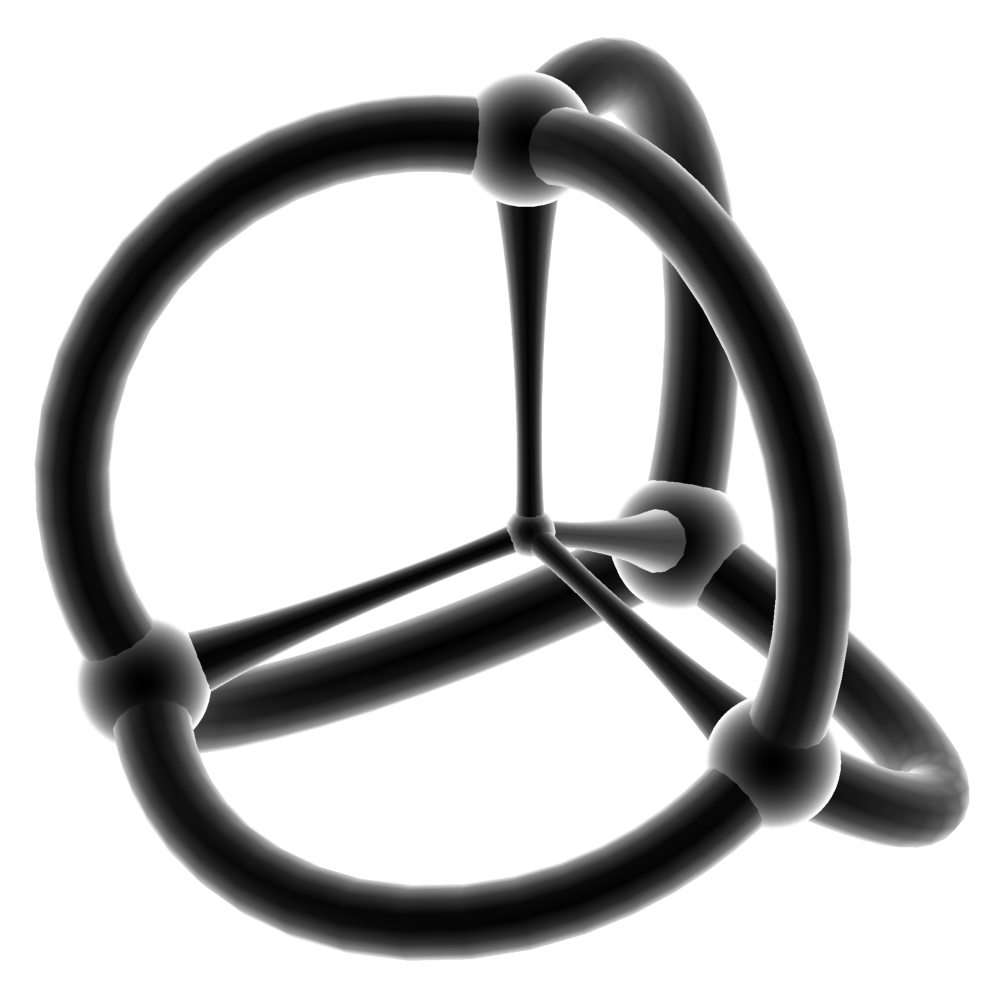
\includegraphics[width=4cm]{matematika/obrazky/4simplex.png}
\caption{Pentachoron}
\end{center}
\end{figure}

Nyní přistupme k formální definici úlohy lineárního programování.

\medskip
\ramcek{14cm}{
\noindent{\bf\textsf{Úloha lineárního programování}} \\
Je dán konvexní polytop v prostoru $\mathbb{R}^n$ popsaný $m$ nerovnostmi.
Maticově to můžeme zapsat ve tvaru $Ax\leq b$, kde $A$ je reálná matice
řádu $m\times n$ a $b$ je vektor $m$ reálných čísel. Dále je dán vektor
$c\in\mathbb{R}^n$. Funkce, kterou chceme maximalizovat, je $\sum_{i=1}^n c_ix_i$,
neboli vektorově $c^Tx$.
Ještě navíc hledáme pouze mezi body se všemi souřadnicemi
nezápornými (tj. $x_i\geq 0$ pro $i=1,\dots, n$).
}

\noindent\textsf{Terminologie}
\begin{penumerate}
 \item Vektoru $c$ říkáme {\it cenový vektor}, funkci $c^Tx$ pak {\it účelová funkce}.
 \item Nerovnosti $Ax\leq b$ a $x\geq 0$ jsou {\it omezující podmínky}, vektor $b$ je {\it pravá strana úlohy}.
 \item Konkrétní zadání úlohy lineárního programování (tj. matice $A$ a vektory $b$, $c$) je {\it přípustné},
pokud existuje nějaký bod splňující $x\geq 0$ a $Ax\leq b$. Jinak je zadání {\it nepřípustné}.
 \item Úloha je {\it neomezená}, pokud můžeme účelovou funkcí dosáhnout na přípustných bodech libovolně veliké hodnoty.
Jinak je {\it omezená}.
\end{penumerate}

\begin{veta}
Pro přípustnou a omezenou úlohu lineárního programování\,\footnote{Tedy existuje alespoň jedno řešení
a účelová funkce je shora omezená.} existuje bod, ve kterém účelová funkce nabývá maxima. Těchto
bodů obecně může být více a říkáme jim optimální řešení.
\end{veta}

\subsection{Simplexová metoda}

Simplexová metoda je označení pro algoritmus řešící úlohu lineárního programování. Byla publikována
v roce 1947 jedním ze zakladatelů lineárního programování američanem Georgem Dantzigem.

\medskip
\begin{center}
{\bf\textsf{Idea}}
\end{center}
\ramcek{14cm}{
Zkonstruujeme přípustné řešení v některém vrcholu polytopu. Poté jdeme po hranách do vrcholů
s vyšší hodnotou účelové funkce.}

Omezující podmínku $Ax\leq b$ tedy změníme na $Ax=b$. Toho docílíme přidáním jedné nezáporné proměnné pro každou podmínku ( $\sum{x}<b$ je totiž ekvivalentní $\sum{x}+y=b$ kde $y\in\mathbb{R}^+$). Tuto úpravu lze také zapsat jako $A:=(A\ I)$. Dále předpokládáme, že matice $A$ má lineárně nezávislé řádky.
Pro podmnožinu indexů $I\subseteq \{1, 2, \dots, n\}$
označme $A_I$ matici $A$, ze které ponecháme pouze sloupce, které jsou v~$I$. Analogicky pro libovolný vektor $w\in\mathbb{R}^n$
označme jako $w_I$ vektor, z něhož ponecháme jenom souřadnice z~$I$ (má dimenzi $n-|I|$).

\ramcek{14cm}{
{\it Báze} (a to nemá nic společného s bází vektorového prostoru) je libovolná podmnožina indexů $B\subseteq \{1, 2, \dots, n\}$ taková, že matice $A_B$ je regulární.
Navíc řekneme, že báze je {\it přípustná}, pokud rovnice $A_Bx_B=b$ má nezáporné řešení.
Vektor $x\in\mathbb{R}^n$ je tzv. {\it bazické řešení}\,\footnote{Někdy též bázové řešení.}, pokud existuje báze $B$ taková, že
$A_Bx_B=b$ a $x_i=0$ pro každé $i\in\{1,2,\dots,m\}\backslash B$.
}
Poznamenejme jen, že bazické řešení ještě nemusí být přípustné. Je-li navíc i přípustné,
říkáme mu přirozeně {\it přípustné bazické řešení}. Proměnným $x_j$ pro $j\in B$, kde
$B$ je báze, říkáme bazické.

\begin{veta}
Nechť $x\in\mathbb{R}^n$ je přípustné řešení. Pak $x$ je bazické řešení, právě když
sloupce matice $A$ odpovídající kladným proměnným jsou lineárně nezávislé.
\end{veta}
%\begin{dukaz}
%Jako $K$ označme množinu těch indexů, pro které je $x_j>0$. Implikace $\Rightarrow$ je jednoduchá,
%neboť je-li $x$ bazické řešení, pak existuje báze $B$ tak, že $A_B$ je regulární a $x_{[n]\backslash B}=0$.
%Jelikož jsou ale všechny souřadnice $x$ vně $B$ nulové, je nutně $K\subseteq B$, a tedy $A_K$ je rovněž regulární.
%Nyní ukažme implikaci $\Leftarrow$.
%\end{dukaz}

\begin{veta}
Nechť $B$ je $m$--prvková indexová množina $B\subseteq \{1,\dots, n\}$ a $A_B$ je regulární. Pak existuje
nejvýše jedno přípustné bazické řešení $x$ ($x_i\neq 0 \Leftrightarrow i\in B$).
\end{veta}

Mezi první tvrzeními jsme uvedli, že má-li daná úloha lineárního programování nějaké přípustné
řešení a je-li zároveň účelová funkce na množině přípustných řešení omezená, pak existuje
optimální řešení (tj. nabývá se maxima). Dá se ale dokázat dokonce následující.

\ramcek{14cm}{
\begin{veta}
Má-li daná úloha optimální řešení, pak i některé bazické řešení je optimální.
\end{veta}}
Tato věta má obrovskou důležitost, neboť je jasné, že {\bf bazických řešení je jen konečně mnoho}.
Ukažme si fungování simplexové metody na konkrétním příkladu.
\begin{priklad}
Maximalizujte funkci $z(x_1,\dots,x_5) = x_1+x_2$ za omezujících podmínek $x_i\geq 0$ ($i=1,\dots, 5$) a
\begin{center}
\fbox{
\begin{tabular}{rrrrrl}
$-x_1$ & $+x_2$ & $+x_3$ & & & $=1$     \\
$+x_1$ & & & $+x_4$ &  & $=3$       \\
& $+x_2$ & & & $+x_5$ & $=2$       \\
\end{tabular}}
\end{center}
\end{priklad}

\begin{proof}[Řešení]
Nejprve najdeme libovolné přípustné bazické řešení. Matice $A$ a vektor $b$ této úlohy jsou ze zadání
\[
A=
\left(
\begin{array}[h]{ccccc}
-1 & 1 & 1 & 0 & 0      \\
1 & 0 & 0 & 1 & 0       \\
0 & 1 & 0 & 0 & 1
\end{array}\right),\quad
b=\left(\begin{array}[h]{c}
   1 \\ 3 \\ 2
  \end{array}\right)
\]
a $m=3, n=5$. Vidíme tedy, že jedním z bazických řešení je $R_1 = (0,0,1,3,2)^T$. Odpovídající
báze indexů je $B=\{3,4,5\}$ (matice $A_B$ je jednotková, a tedy regulární). Na základě tohoto
vytvoříme tzv. {\it simplexovou tabulku} (počáteční přípustnou tabulku) tak, že vyjádříme bazické proměnné
pomocí nebazických a přidáme jeden řádek s vyjádřenou účelovou funkcí pomocí nebazických proměnných.
\[
\begin{array}{c|ccc}
x_3=& 1 & +x_1 & -x_2   \\
x_4=& 3 & -x_1 &        \\
x_5=& 2 & & -x_2        \\
\hline
z=& & x_1 & +x_2
\end{array}, \quad R_1 = (0,0,1,3,2)^T, \quad z=0
\]

V bodě $R_1$ je $z(R_1) = 0$. Nyní budeme, jak bylo naznačeno, postupně zvyšovat
hodnotu funkce $z$, dokud nezjistíme, že jsme nalezli optimální řešení. Hodnotu funkce $z$ budeme
zvětšovat zvětšením hodnoty některé nebazické (volné) proměnné.

Ponechejme $x_1=0$ a zvětšeme $x_2$ z $0$ na $1$ (jednička je nejlepší možná, viz první rovnici a $x_3\geq 0$).
Pak pomocí tabulky dostaneme nové přípustné řešení, konkrétně $R_2=(0,1,0,3,1)^T$. Z první rovnice teď
vyjádříme $x_2$:
\[
x_2 = 1+x_1-x_3
\]
a nahradíme touto rovnicí původní první rovnici $x_3=1+x_1-x_2$. Toto řešení odpovídá bázi $B=\{2,4,5\}$.
Snadno zjistíme, že $z(R_2) = 0+1 = 1$. Nyní se stalo, že proměnná $x_2$ nahradila proměnnou $x_3$ v bázi.
Tomuto procesu říkáme, že proměnná $x_2$ \uv{vstoupila do báze}, $x_3$ z ní \uv{vystoupila}.
\smallskip

Dostáváme tak novou simplexovou tabulku
\[
\begin{array}{c|ccc}
x_2=& 1 & +x_1 & -x_3   \\
x_4=& 3 & -x_1 &        \\
x_5=& 1 & -x_1& +x_3        \\
\hline
z=& 1& +2x_1 & -x_3
\end{array}, \quad R_2=(0,1,0,3,1)^T, \quad z=1
\]
Nyní budeme zvyšovat $x_1$. První rovnice $x_1$ neomezuje, druhá říká $x_1\leq 3$ a třetí nyní říká $x_1\leq 1$
(jelikož $x_3=0$). Položme tedy $x_1=1$. Dostáváme nové řešení $R_3=(1,2,0,2,0)^T, z(R_3) = 3$. Proměnná
$x_1$ vstoupí do báze místo proměnná $x_5$. Nová báze je $B=\{1,2,4\}$.
\smallskip

Dostáváme další simplexovou tabulku
\[
\begin{array}{c|ccc}
x_1=& 1 & +x_3 & -x_5   \\
x_2=& 2 &  &  -x_5       \\
x_4=& 2 & -x_3& +x_5        \\
\hline
z=& 3& +x_3 & -2x_5
\end{array}, \quad R_3=(1,2,0,2,0)^T, \quad z=3
\]
Zvětšíme $x_3$ z $0$ na $2$ ($x_3\leq 2$ plyne ze třetí rovnice tabulky) a tím obdržíme
další řešení $R_4=(3,2,2,0,0)^T$, báze je $B=\{1,2,3\}$, $z(R_4)=5$. Odpovídající nová
simplexová tabulka je
\[
\begin{array}{c|ccc}
x_1=& 3 & -x_4 &    \\
x_2=& 2 &  &  -x_5       \\
x_3=& 2 & -x_4& +x_5        \\
\hline
z=& 5& -x_4 & -x_5
\end{array}, \quad R_4=(3,2,2,0,0)^T, \quad z=5
\]
Nyní je jasné, že libovolné zvýšení volné proměnné $x_4$ nebo $x_5$ sníží hodnotu účelové funkce.
Z konstrukce simplexové metody plyne, že řešení $R_4$ je již optimální, neboť jsme prováděli pouze
ekvivalentní rovnicové úpravy. Optimálním řešením dané úlohy je tedy bod $(3,2,2,0,0)$.



\end{proof}




Časová složitost simplexové metody je $O(2^n)$.
Jeden z nejhorších případů můžeme vzít $n$--dimenzionální krychli,
která má přesně $2^n$ vrcholů. Na této krychli algoritmus
může postupně navštívit všechny její vrcholy. 

Simplexová metoda nachází uplatnění převážně při řešení optimalizačních úloh v inženýrství nebo ekonomii.

\subsection{Duální úloha}

Problém lineárního programování tak, jak byl popsán výše, označujeme jako {\it primární}.
Ke každému primárnímu problému můžeme zkonstruovat {\it duální úlohu}. Připomeňme, že
primární úloha byla najít
\[
\max\{ c^Tx : x\in\mathbb{R}^n, Ax\leq b, x\geq 0 \}.
\]
Duální úloha k této pak je najít
\[
\min\{ b^Ty : y\in\mathbb{R}^m, A^Ty\geq c, y\geq 0 \}.
\]
Základem teorie duality lineárního programu jsou následující dvě věty -- {\it (Slabá) věta o dualitě}.

\begin{vetaN}{Slabá věta o dualitě}
Pokud je $x$ přípustné řešení primární úlohy a $y$ přípustné řešení duální úlohy, pak
hodnota duální účelové funkce v bodě $y$ je alespoň tak veliká jako hodnota primární účelové
funkce v bodě $x$.
\end{vetaN}

\begin{vetaN}{Věta o dualitě}
Nechť $x_*$ je optimální řešení primární úlohy. Pak existuje optimální řešení $y_*$ duální úlohy takové, že
\[
c^Tx_* = b^Ty_*.
\]
\end{vetaN}
\bigskip

\noindent{\bf\textsf{Duální úloha ze života}}

\dots 

%Mějme malou pekárničku na rohu ulice a školačku Kačenku, která si chce koupit
%něco dobrého ke~svačině. V pekárničce prodávají dva druhy zboží -- bábovky a pařížské dorty.
%Bábovka stojí 80 Kč, pařížský dort 50 Kč. Pekárníčku vlastní jedna hodná paní ze sousedství, a proto
%si můžete vzít i jen kousek bábovky nebo dortíku. Na pařížský dortík jsou potřeba
%3 unce čokolády, 2 unce cukru a 2 unce krému. Na bábovku pak jsou potřeba
%4 unce cukru a 5 uncí krému. Jelikož ale Kačenka dá na správnou výživu,\footnote{A daří se jí to převelice.}
%ví, že musí jíst hodnotně, a proto si stanovila, že chce, aby její svačinka měla alespoň 6
%uncí čokolády, 10 uncí cukru a 8 uncí krému. Jelikož má ale malinkatou peněženku, do které se jí
%nevešelo moc penízků, chce, aby si svačinku splňující daná kritéria nakoupila co nejlevněji.
%Pomůžete milé Kačence?
%\medskip


%Zaveďme nyní $m$ nových proměnných $x_{n+1}, x_{n+2}, \dots, x_{n+m}$ pomocí vztahu
%\[
%x_{n+i} = b_i - \sum_{j=1}^n A_{ij}x_j,\quad i=1, 2, \dots, m
%\]
%a přidejme pro každou takto nově vytvořenou proměnnou ještě omezující podmínku $x_{n+i}\geq 0$.
%Každá proměnná $x_{n+i}$ je tedy jakousi \uv{chybou} (rozdílem) hodnoty pravé strany
%a hodnoty levé strany $i$--té nerovnosti.

\newpage
\def\Nat{\mathbb{N}}
\def\Real{\mathbb{R}}
\def\Pot{\mathcal{P}}

\section{Diskrétní matematika}

\begin{pozadavky}
\begin{pitemize}
\item Uspořádané množiny
\item Množinové systémy, párování, párování v bipartitních grafech (systémy různých reprezentantů)
\item Kombinatorické počítání
\item Princip inkluze a exkluze
\item Latinské čtverce a projektivní roviny.
\end{pitemize}
\end{pozadavky}

\subsection{Uspořádané množiny}

\begin{definiceN}{Kartézský součin}
Nechť $X$ a $Y$ jsou množiny. Symbolem $X \times Y$ označíme množinu všech uspořádaných dvojic tvaru $(x,y)$, kde $x \in X$ a $y \in Y$. Formálně zapsáno:
$X \times Y = \{ (x,~y); x \in X, y \in Y \}$ se nazývá \emph{kartézský součin} množin $X$ a $Y$.

Kartézský součin $X \times X$ někdy značíme jako $X^2$. 
\end{definiceN}

\begin{definiceN}{relace}
Relace R je množina uspořádaných dvojic. Jsou-li $X$ a $Y$ množiny, nazývá se libovolná podmnožina kartézského součinu $X \times Y$ \emph{relací} mezi $X$ a $Y$. Zdaleka nejdůležitější případ je $X=Y$. V takovém případě mluvíme o relaci na $X$, což je tedy libovolná podmnožina $X^2$.

Náleží-li $(x,y)$ relaci $R$, tedy $(x,y) \in R$, říkáme, že $x$ a $y$ jsou v relaci $R$. Značíme $xRy$.
\end{definiceN}

\begin{definiceN}{druhy relací}
Relace $X$ může být:
\begin{pitemize}
	\item \emph{reflexivní}, jestliže pro každné $x \in X$ platí $xRx$
	\item \emph{ireflexivní}, jestliže platí $xRy\ \Rightarrow\ x\neq y$
	\item \emph{symetrická}, jestliže $xRy \Rightarrow yRx$
	\item \emph{tranzitivní}, jestliže $xRy \wedge yRz \Rightarrow xRz$
	\item \emph{antisymetrická}, jestliže $xRy \wedge yRx \Rightarrow x=y$
\end{pitemize}
\end{definiceN}

\begin{definiceN}{ekvivalence}
Řekneme, že relace $R$ na $X$ je \emph{ekvivalence} na $X$, jestliže je symetrická, reflexivní a tranzitivní.
\end{definiceN}

\begin{definiceN}{uspořádání, uspořádaná množina}
\emph{Uspořádání} na nějaké množině $X$ je každá relace na $X$, která je reflexivní, tranzitivní a antisymetrická. \emph{Uspořádaná množina} je dvojice $(X,R)$, kde $X$ je množina a $R$ je uspořádání na $X$.

Pro uspořádání se používá značení $\le$ nebo $\preceq$. Pro každé uspořádání lze odvodit \uv{ostrou nerovnost} $<$ nebo $\prec$, kde platí, že $x<y \Leftrightarrow x \le y \wedge x \neq y$.
\end{definiceN}

\begin{priklady}
Uspořádané množiny:
\begin{pitemize}
    \item $(\Nat,\leq)$
    \item $(\Nat,|)$, kde \uv{$|$} je relace \uv{dělí}
    \item $(\Pot(X),\subseteq)$, kde $\Pot(X)$ označuje množinu všech podmnožin a $\subseteq$ normální množinovou inkluzi
    \item orientovaný acyklický graf $(V,E)$ s relací $\rho:(a,b)\in\rho \equiv^{def} \textit{ existuje cesta z }a\textit{ do }b $
\end{pitemize}
\end{priklady}

\begin{definiceN}{lineární uspořádání}
\emph{Lineární uspořádání} je takové uspořádání, kde pro každé dva prvky $x$ a $y$ platí buď $x \leq y$ nebo $y \leq x$. Někdy se také nazývá \emph{úplné uspořádání}.

Uspořádání, které není úplné, nazýváme \emph{částečným uspořádáním}.
\end{definiceN}

\begin{definiceN}{bezprostřední přechůdce}
\emph{Bezprostřední předchůdce} prvku $y$ je takový prvek $x$, pro který platí $x < y$, a neexistuje žádné takové $t$, že $x < t < y$.
\end{definiceN}

\begin{poznamkaN}{Hasseův diagram}
Při znázorňovaní se uspořádaná množina zakresluje pomocí bodů a šipek, jako kterákoliv jiná relace. Protože těchto šipek by bylo mnoho, vychází se z tranzitivity a znázorňují se šipky pouze mezi prvky a jejich bezprostředními předchůdci. Přijmeme-li navíc konvenci, že v obrázku povedou všechny šipky nahoru, není třeba zakreslovat směr šipek, pouze spojnice bodů. Takovéto znázornění se pak nazývá \emph{Hasseův diagram}.
\end{poznamkaN}

\begin{poznamkaN}{uspořádání na kartézském součinu}
Mám-li dvě množiny $A$ a $B$ a na nich uspořádání $\leq_A$ a $\leq_B$ můžu definovat \uv{složené uspořádání}
\begin{pitemize}
    \item \uv{po složkách} -- $(a_1,b_1)\leq(a_2,b_2)\equiv^{\textrm{def}} a_1\leq_A a_2 \wedge b_1 \leq_B b_2$
    \item \uv{lexikograficky} -- $(a_1,b_1)\leq(a_2,b_2)\equiv^{\textrm{def}} a_1\leq_A a_2 \vee ( a_1=a_2 \wedge b_1\leq_B b_2)$
\end{pitemize}
\end{poznamkaN}

\begin{definice}
Říkáme, že $(X,R)$ a $(Y,P)$ jsou \emph{isomorfní uspořádané množiny}, pokud existuje nějaké vzájemně jednoznačné zobrazení $f:X \rightarrow Y$ takové, že pro každé $x,y \in X$ platí $xRy$ právě když $f(x) P f(y)$.
\end{definice}

\begin{definiceN}{Předuspořádání}
\emph{Předuspořádání} nazveme každou relaci, která je reflexivní a transitivní (nebudeme tedy požadovat antisymetrii -- mohou vznikat \uv{cykly}).
\end{definiceN}

\begin{poznamka}
Mám-li množinu $X$ s relací $\sim$, která je předuspořádání, potom relace $\sim$ je uspořádání na množině $X/\rho$ (rozklad podle tříd ekvivalence $\rho$), kde $a\rho b\equiv (a\sim b \wedge b\sim a)$.
\end{poznamka}

\begin{definice}
\emph{Nezávislý systém $M$ podmnožin množiny $X$} je podmnožina $P(X)$ taková, že každé dvě množiny $A, B \in M$ jsou neporovnatelné relací náležení.
\end{definice}

\begin{vetaN}{Spernerova}
Libovolný nezávislý systém podmnožin $n$-prvkové množiny má nejvýš $\binom{n}{\lfloor\frac{n}{2}\rfloor}$ množin.
\end{vetaN}

TODO: Patří sem dobré uspořádání a Zernelova věta??? (to by znamenalo přidat sem i supremum, infimum, řetězec, nejmenší a největší prvek)

\subsection{Množinové systémy, párování, párování v bipartitních grafech (systémy různých reprezentantů)}

\begin{definice}
Nechť $X$ a $I$ jsou množiny. \emph{Množinovým systémem nad $X$} nazveme $|I|$-tici $M=\{M_i; i \in I\}$, kde $M_i \subseteq X$

Je tedy možné, aby se tam táž množina objevila víckrát.
\end{definice}

\begin{definiceN}{systém různých reprezentantů}
\emph{Systém různých reprezentantů} (SRR) je funkce $f: I \rightarrow X$ taková, že $\forall i \in I: f(i) \in M_i$ a $f$ je prostá.

Jinými slovy, SRR je výběr jednoho prvku z každé množiny $M_i$ tak, že všechny vybrané prvky jsou navzájem různé. Obecně se tedy neuvažují nekonečné systémy.
\end{definiceN}

\begin{definiceN}{párování}
\emph{Párování v grafu} $G$ je množina hran $F \subseteq E(G)$ taková, že každý vrchol grafu $G$ patří nejvýše do jedné hrany z $F$.

Ekvivalentní definice jsou přes stupeň vrcholu (každý vrchol má stupeň nejvýše 1) nebo přes disjunktnost hran (každé dvě jsou disjunktní - žádné dvě nemají společný vrchol).
\end{definiceN}

\begin{definiceN}{bipartitní graf}
\emph{Bipartitní graf} je takový graf $G$, kde množinu vrcholů $V(G)$ můžeme rozdělit na dvě disjunktní podmnožiny $V_1$ a $V_2$ takové, že každá hrana z $E(G)$ spojuje vždy vrchol z $V_1$ s vrcholem z $V_2$.
\end{definiceN}

\begin{definice}
\emph{Incidenčním grafem} množinového systému $M$ nad množinou $X$ nazveme bipartitní graf
$$
B_M = \left( I \cup X, \left\{ \{i,x\}, x \in M_i \right\} \right)
$$
\noindent
V podstatě si každý prvek z $X$ i každý index $I$ označíme vrcholem a spojíme každý index $i$ s prvky $x$, které náleží do $M_i$. Z incidenčního grafu pak lze nahlédnout existenci SRR - ten existuje, právě když v incidenčním grafu existuje párování velikosti $|I|$.
\end{definice}

\begin{vetaN}{Hallova}
Systém různých reprezentantů v $M$ existuje, právě když pro každou $J \subseteq I$ je $$\left| \bigcup_{j \in J} M_j\right| \ge |J|$$
\end{vetaN}

\begin{definiceN}{perfektní párování}
\emph{Perfektním párováním} nazveme párování $M$ v grafu $G$, pro které platí $$|M| = \frac{|V(G)|}{2}$$

\noindent
Tedy perfektní párování je takové, kde je každý vrchol spárovaný s nějakým jiným vrcholem. Dalším důležitým pojmem je \emph{maximální párování}, což je v podstatě nejlepší možné párování (pokrývá největší možný počet vrcholů), jakého jsme v daném grafu schopni dosáhnout.
\end{definiceN}


\begin{vetaN}{O párování v bipartitním grafu}
Buď $G=(A\cup B,E)$ graf se dvěma partitami $A$ a $B$ a $E$ neprázdná množina hran. Jestliže platí $\deg u \geq \deg v\ \forall u\in A,\forall v\in B$, potom existuje párování velikosti $|A|$. Díky tomu pokud má bipartitní graf všechny vrcholy stejného stupně, pak má perfektní párování.

\begin{dukaz}
Převede se na Hallovu větu s použitím \uv{okolí} vrcholů (tj. bodů přímo spojených s vrcholem hranou).
\end{dukaz}
\end{vetaN}

\begin{vetaN}{Tutteova}
Graf $(V,E)$ má perfektní párování, právě když pro každou množinu vrcholů $A\subseteq V$ platí:
$$c_l(G\setminus A)\leq |A|$$
(tj. počet komponent souvislosti s lichých počtem vrcholů v indukovaném podgrafu je menší než velikost množiny vrcholů). Této vlastnosti se také někdy říká \emph{Tutteova podmínka}.
\end{vetaN}

\begin{algoritmusN}{Edmondsův algoritmus na perfektní párování}
Vstupem algoritmu je graf $G=(V,E)$ a libovolné párování $M$ (i prázdné). Výstupem je párování $M'$, které alespoň o 1 větší než $M$, pokud je něčeho takového možné dosáhnout. Postup výpočtu:
\begin{penumerate}
    \item Vybudujeme maximální možný \uv{Edmondsův les} párování $M$ -- do nulté hladiny umístíme volné vrcholy a prohledáváním do šířky sestrojíme max. strom takový, že se střídají párovací a nepárovací hrany (mezi sudou a lichou hladinou jen nepárovací, mezi lichou a sudou jen párovací).

Některé vrcholy se v lese vůbec neobjeví -- nazveme je \uv{kompost}. Ty jsou už nějak spárovány mezi sebou a nebudeme je potřebovat.
    \item Pokud existuje hrana mezi sudými hladinami různých stromů, máme \uv{volnou střídavou cestu} (tj. cestu liché délky mezi 2 volnými vrcholy, na které se střídají nepárovací a párovací hrany), na níž můžeme zalternovat hrany párování a to tak zvětšit o 1 a skončit.
    \item Pokud existuje hrana mezi sudými hladinami téhož stromu, máme \uv{květ} (tj. kružnici liché délky, na které se střídají párovací a nepárovací hrany). Květ můžeme zkontrahovat a algoritmus rekurzivně pustit na takto získaný graf. Pokud dostaneme
    \begin{penumerate}
	\item staré párování beze změny, vrátíme $M'=M$
	\item jiné (větší) párování $\hat M$, prohodíme párování na cestě v $\hat M$ od vrcholu květu v nejvyšší hladině (kam jsme květ zkontrahovali) k volnému vrcholu a přidáme květ zpátky (a párování sedí a je větší než $M$)
    \end{penumerate}
    \item Není-li žádná hrana mezi sudými hladinami, vydej $M'=M$.
\end{penumerate}
\par\medskip\noindent
Hlavní algoritmus jen opakuje výše popsaný krok, dokud vrací větší párování než bylo předchozí. Celková složitost jednoho kroku je $O((m+n)n)$ a pro celý algoritmus $O((m+n)n^2)$.
\end{algoritmusN}


\subsection{Kombinatorické počítání}

\begin{veta}
Nechť $N$ je nějaká $n$-prvková množina a $M$ je $m$-prvková množina ($m > 0$). Potom počet všech zobrazení $f: N \rightarrow M$ je $m^n$.
\end{veta}

\begin{veta}
Libovolná $n$-prvková množina $X$ má právě $2^n$ podmnožin.
\end{veta}

\begin{veta}
Nechť $n>0$. Každá $n$-prvková množina má právě $2^{n-1}$ podmnožin sudé velikosti a právě $2^{n-1}$ podmnožin liché velikosti.
\end{veta}

\begin{veta}
Pro $m,n \ge 0$ existuje právě $m(m-1)(m-2) \dots (m-n+1)$ prostých zobrazení $n$-prvkové množiny do $m$-prvkové množiny.
\end{veta}

\begin{definice}
Prostá zobrazení množiny $X$ do sebe se nazývá \emph{permutace množiny} $X$. Tato zobrazení jsou zároveň na.

Permutace si můžeme představit jako přerovnání množiny - např. $\{4 2 1 3\}$ je permutací množiny $\{1 2 3 4\}$. Jiný zápis permutací je pomocí jejich cyklů (\emph{cyklus} v permutaci je pořadí prvků, kde začnu u nějakého prvku, pokračuji jeho obrazem v permutaci a toto opakuji, dokud nenarazím na první prvek). U cyklů znázorníme každý prvek množiny jako bod. Z každého bodu vychází a do každého vchází právě po jedné šipce. Šipka vycházející z prvního prvku množiny ukazuje na první prvek permutace, šipka z druhého prvku množiny na druhý prvek permutace atd. Zápis se pak provádí tak, že každou kružnici zapíšeme po řadě zvlášť (např. $p=((1,4,5,2,8)(3)(6,9,7))$ je zápis permutace $(4 8 3 5 2 9 6 1 7)$.
\end{definice}

\begin{vetaN}{Faktoriál}
Počet permutací na $n$-prvkové množině je $n\cdot(n-1)\cdot\dots\cdot 1$. Toto číslo pojmenujeme \emph{faktoriál} $n$ a značíme $n!$.
\end{vetaN}

\begin{definiceN}{Binomické koeficienty}
Nechť $n \ge k$ jsou nezáporná celá čísla. \emph{Binomický koeficient} neboli kombinační číslo $\binom{n}{k}$ (čteme $n$ nad $k$) je funkce proměnných $n$, $k$, daná jako $$\binom{n}{k}=\frac{n(n-1)(n-2)\dots(n-k+1)}{1 \cdot 2 \cdot \dots \cdot k}=\frac{\prod^{k-1}_{i=0} (n-i)}{k!}$$ nebo $$\binom{n}{k}=\frac{n!}{k!(n-k)!}$$
\end{definiceN}

\begin{definice}
Nechť $X$ je množina a $k$ je nezáporné celé číslo. Pak $\binom{X}{k}$ budeme značit \emph{ množinu všech $k$-prvkových podmnožin} množiny $X$.
\end{definice}

\begin{veta}
Pro každou konečnou množinu $X$ je počet všech jejích $k$-prvkových podmnožin roven $\binom{|X|}{k}$.
\end{veta}

\begin{vetaN}{Vlastnosti kombinačních čísel}
Platí:
$$
\binom{n}{k} = \binom{n}{n-k}
$$

$$
\binom{n-1}{k-1} + \binom{n-1}{k} = \binom{n}{k}
$$

\begin{dukaz}
První je zřejmé ze vzorce pro kombinační čísla, druhé se ukaže jednoduše pro použití komb. čísel -- mějme množinu $X$ a v ní prvek $a$. Kolik je podmnožin $X$ obsahujících, resp. neobsahujících $a$?
\end{dukaz}
\end{vetaN}

\begin{dusledek}
Z druhé vlastnosti plyne vzhled \emph{Pascalova trojúhelníku}, tedy že v $n+1$. řádku jsou vždy právě binomické koeficienty $\binom{n}{0},\binom{n}{1},\dots,\binom{n}{n}$.
\end{dusledek}

\begin{vetaN}{O počtu způsobů zápisu}
Nezáporné celé číslo $m$ lze zapsat jako součet $r$ nezáporných sčítanců právě $\binom{m+r-1}{r-1}$ způsoby.

\begin{dukaz}
Důkazem je onen pokus s rozdělováním $m$ kuliček mezi $r$ přihrádek (nebo spíš vkládání přihrádek mezi kuličky v řadě).
\end{dukaz}
\end{vetaN}

\begin{vetaN}{Binomická věta}
Pro nezáporné celé číslo $n$ a libovolná $x,y\in\Real$ platí: $$(x+y)^n=\sum_{k=0}^{n} \binom{n}{k} x^k y^{n-k}$$
\end{vetaN}

\begin{vetaN}{Multinomická věta}
Pro libovolná čísla $x_1,\dots,x_m\in\Real$ a $n\in\Nat_0$ platí: 
$$(x_1+\dots+x_m)^n=\sum_{\genfrac{}{}{0pt}{}{k_1+\dots+k_m=n}{k_1,\dots,k_m\geq 0}}\binom{n}{k_1,\dots,k_n}x_1^{k_1}x_2^{k_2}\cdot\dots\cdot x_m^{k_m}$$
kde ta věc uprostřed v tom vzorci je \emph{multinomický koeficient}, definovaný:
$$\binom{n}{k_1,\dots,k_n}=\frac{n!}{k_1!k_2!\dots k_n!}$$
\end{vetaN}

\subsection{Princip inkluze a exkluze}

\begin{vetaN}{Princip inkluze a exkluze}
Pro každý soubor $A_1, A_2, \dots, A_n$ konečných množin platí

$$
\left| \bigcup_{i=1}^{m}A_i \right| = \sum_{k=1}^{n} (-1)^{k-1} {\sum_{I \in \binom{\{1,2,\dots,n\}}{k}} {\left| \bigcap_{i \in I} A_i \right|} }
$$
\end{vetaN}

\begin{dukaz}
Nechť x je libovolný prvek $A_1 \cup A_2 \cup \dots \cup A_n$. Kolikrát přispívá x vlevo a kolikrát vpravo?

\emph{Vlevo}: jednou - triviální
\emph{Vpravo}: Nechť j ($1 \le j \le n$) označuje počet množin $A_i$, do kterých patří $x$. Můžeme množiny přejmenovat aby platilo $x~\in~A_1,~A_2,~\dots,~A_j$ a $x~\notin~A_{j+1},~\dots,~A_n$. Prvek se tedy objevuje v průniku každé $k$-tice množin $A_1,~A_2,~\dots,~A_j$ (a v žádných jiných). Protože existuje právě $\binom{j}{k}$ $k$-prvkových podmnožin $j$-prvkové množiny, bude se $x$ objevovat v $\binom{j}{k}$ průnicích $k$-tic vybraných ze všech $n$ prvků. Velikosti $k$-tic jsou přitom započteny se znaménkem $(-1)^{k-1}$, tudíž $x$ na pravé straně přispívá veličinou

\begin{align*}
j - \binom{j}{2} & + \binom{j}{3} - \dots + (-1)^{j-1}\binom{j}{j} =\\
& = 1 - \binom{j}{0} + \binom{j}{1} - \binom{j}{2} \dots + (-1)^{j-1}\binom{j}{j} =\\
& = 1 - \sum_{i=0}^{j} \binom{j}{i} (-1)^{i}  = 1 - (1-1)^{j} = 1
\end{align*}
\begin{flushright}
$\square$
\end{flushright}
\end{dukaz}


\subsection{Latinské čtverce a projektivní roviny}

\begin{definiceN}{Projektivní rovina}
\emph{Konečná projektivní rovina} je množinový systém $(B,P)$, kde $B$ je konečná množina a $P$ je systém podmnožin množiny $B$, splňující:
\begin{penumerate}
	\item $\forall p \neq p' \in P: |p \cap p'| = 1$
	\item $\forall x \neq y \in B~\exists p \in P: x,y \in p$
	\item $\exists \textit{ 4 body } a,b,c,d \in B: \forall p \in P: |\{a,b,c,d\} \cap p| \leq 2$
\end{penumerate}

Projektivní rovinu si lze představit jako množinu bodů $B$ a množinu \emph{přímek} $P$ (jak se ostatně prvky těchto množin nazývají). Pak si lze podmínky představit takto:
\begin{penumerate} 
    \item Každé dvě přímky se protínají právě v jednom bodě. 
    \item Pro každé dva různé body $x$ a $y$ existuje přímka, která jimi prochází. 
    \item Existují čtyři body tak, že žádné 3 z nich neleží na jedné přímce (body v obecné poloze).
\end{penumerate}
\end{definiceN}

\begin{veta}
Buď $(B,P)$ projektivní rovina. Potom všechny její přímky mají stejný počet bodů, tedy $\forall p,q \in P: |p| = |q|$
\end{veta}

\begin{definice}
\emph{Řád projektivní roviny} $(B, P)$ je číslo $|p|-1$, kde $p$ je libovolná přímka z $P$ ($p \in P$).
\end{definice}

\begin{veta}
Nechť $(B,P)$ je projektivní rovina řádu $n$. Potom platí, že každým bodem prochází právě $n+1$ přímek a $|B|=|P|=n^2+n+1$
\end{veta}

\begin{veta}
Jestliže $n=p^2$, kde $p$ je prvočíslo, pak existuje konečná projektivní rovina řádu $n$.
\end{veta}

\begin{definiceN}{Latinský čtverec}
\emph{Latinský čtverec} řádu $n$ je matice $A \in \{1, \dots, n\}^{n \times n}, \;\forall i, j \neq j': A_{ij}~\neq~A_{ij'}$ a $A_{ji}~\neq~A_{j'i}.$

V podstatě se jedná o čtverec $n$ krát $n$, kde v každém řádku i sloupci jsou vepsaná všechna čísla od $1$ do $n$.
\end{definiceN}

\begin{definice}
Mějme dva latinské čtverce $A, B$ stejných rozměrů $n \times n$. Pak řekneme, že je \emph{ortogonální} (značíme $A \bot B$), jestliže platí:
$$\forall a,b \in \{1,\dots,n\} \;\exists i,j: A_{ij}=a, B_{ij}=b$$

Pokud tedy ty dva latinské čtverce \uv{položíme přes sebe}, vznikne nám na každé pozici dvojice čísel od $1$ do $n$ s tím, že každá dvojice je unikátní.
\end{definice}

\begin{veta}
Nechť $M$ je množina latinských čtverců řádu $n$, z nichž každé dva jsou navzájem ortogonální. Potom $|M| \le n-1$
\end{veta}

\begin{veta}
Pro $n \ge 2$, projektivní rovina řádu $n$ existuje právě tehdy, když existuje soubor $n-1$ vzájemně ortogonálních latinských čtverců řádu $n$.
\par\medskip
\begin{dukaz}
\begin{enumerate}
    \item \emph{Implikace $\Leftarrow$:} Vezmu jednu -- \uv{vnější} -- přímku projektivní roviny. Na ní leží $n+1$ bodů, které nazvu $A_0,\dots,A_n$. Přímky jdoucí z krajních bodů $A_0$ a $A_n$ tvoří mřížku (nazvu ji $T$) -- protínají se v $n^2$ bodech. 

Potom každý z vnitřních bodů $A_i\ (1 ? i ? n-1)$ definuje lat. čtverec: každá přímka jdoucí z nějakého z vnitřních bodů $A_i$ se s přímkami z $A_0$ a z $A_n$ protne právě jednou a každé 2 přímky z $A_i$ prochází mimo vnější přímku různými body. Každá přímka proch. každým řádkem i sloupcem mřížky $T$ právě jednou $\Rightarrow$ dostávám latinský čtverec: 
$$(L^k)_{ij} = l \Leftrightarrow T_{ij} \in p^k_l$$
kde $L^k$ značí $k$-tý lat. čtverec, $T_{ij}$ bod mřížky $T$ na souřadnicích $(i,j)$ a $p^k_l$ $l$-tou přímku jdoucí z bodu $A_k$. 

Čtverce jsou ortogonální - sporem nechť pro mají dva čtverce ($k$-tý a $k'$-tý) na souřadnicích stejnou uspořádanou dvojici hodnot $(a,b)$ na dvou různých místech. Pak by se přímky $p^k_a$ a $p^{k'}_b$ protínaly ve 2 bodech.

    \item \emph{Implikace $\Rightarrow$:} Vytvořím přímku $q$ s body $A_0,\dots,A_n$ a mřížku $T$ o $n\times n$ bodech. Do ní přidám přímky $p_{1,1},\dots,p_{n-1,n}$: 
$$p_l^k = \{A_k\} \cup \{T_{ij} | L^k_{ij} = l \}$$ 
Pak je třeba ověřit axiomy projektivní roviny. 
\end{enumerate}
\end{dukaz}
\end{veta}

\newpage
\section{Teorie grafů}

\begin{poziadavky}
\begin{pitemize}
    \item Základní pojmy teorie grafů, reprezentace grafu.
    \item Stromy a jejich základní vlastnosti, kostra grafu.
    \item Eulerovské a hamiltonovské grafy.
    \item Rovinné grafy, barvení grafů.
\end{pitemize}
\end{poziadavky}

\subsection{Základní pojmy teorie grafů, reprezentace grafu}

\begin{definiceN}{Graf}
Graf $G$ je uspořádaná dvojice $(V,E)$, kde $V$ je nějaká množina a $E$ je množina dvouprvkových podmnožin množiny $V$ (takže neuspořádaných dvojic). Prvky množiny $V$ se jmenují \textbf{vrcholy grafu $G$} a prvky množiny $E$ \textbf{hrany grafu $G.$}
\end{definiceN}

\begin{definiceN}{Orientovaný graf}
$G$ je dvojice $(V,E),$ kde $E$ je podmnožina kartézského součinu $V \times V$. Prvky $E$ (tj. uspořádané dvojice prvků z $V$) nazýváme orientované hrany grafu.
\end{definiceN}

\begin{definiceN}{Symetrizace grafu}
Orientovanému grafu $G=(V,E)$ přiřadíme neorientovaný graf $\mathrm{sym}(G) = (V,\bar E) $ kde $\bar E=\{\{x,y\};$ $(x,y) \in E \lor (y,x) \in E \}.$ Graf $\mathrm{sym}(G)$ se nazývá \textbf{symetrizace} grafu $G.$ \textit{(Z orientovaného grafu se odstraní údaje o směru hran.)}
\end{definiceN}

\begin{definiceN}{Důležité typy grafů}
\begin{pitemize}
\item \textbf{úplný graf $K_n$:} $V=\{1,\dots,n\}, E=\binom{V}{2}$ \textit{(Každý vrchol je spojen hranou s každým např. $K_5$ --- \uv{pentagram}.)}
\item \textbf{kružnice $C_n$:} $V=\{1,\dots,n\}, E=\{\{i, i+1\}; i=1,\dots,n-1\} \cup\{\{1,n\}\}$ \textit{(V~kružnici se nesmí opakovat vrcholy.)}
\item \textbf{cesta $P_n$:} $V=\{0,1,\dots,n\}, E=\{\{i-1,i\}; i=1,\dots,n\}$ \textit{(Jako kružnice, ale bez poslední hrany.)}
\item \textbf{bipartitní graf:} $V=\{u_1,\dots,u_n\} \; \cup \; \{v_1,\dots,v_m\}$, $E \subseteq \{\{u_i,v_j\}; i=1,\dots,n, j=1,\dots,m\}$; v \textbf{úplném bipartitním grafu} je $E = \{\{u_i,v_j\}; i=1,\dots,n, j=1,\dots,m\}$ \textit{(Každý vrchol z jedné partity je spojen hranou pouze s některými (v úplném z každým) vrcholem druhé partity. Např. $K_{3,3}$, úplný bipartitní graf na 3 a 3 vrcholech.)}
\end{pitemize}
\end{definiceN}

\begin{definiceN}{Sled, tah}
Pro graf $G=(V,E)$ definujeme \textbf{sled} jako posloupnost $(v_0,e_1,v_1,\dots,e_n,v_n),$ kde $e_i=\{v_{i-1},v_i\} \in E$ pro $i=1,\dots,n.$ \textbf{Tah} je sled, ve kterém se žádná hrana neopakuje.
\end{definiceN}

\begin{definiceN}{Isomorfismus grafů}
Dva grafy $G, G'$ považujeme za \textbf{isomorfní} (značíme $G\simeq G'$), pokud se liší jen v označení vrcholů a hran, tj. pokud existuje vzájemně jednoznačné zobrazení $f: G \rightarrow G'$ tak, že platí $\{x,y\}\in E \Leftrightarrow \{f(x),f(y)\} \in E'.$
\end{definiceN}

\begin{definiceN}{Podgraf, indukovaný podgraf}
Graf $G$ je \textbf{podgrafem} grafu $G',$ jestliže $V(G)\subseteq V(G')$ a $E(G)\subseteq E(G') \cap \binom{V(G)}{2}$. Pro \textbf{indukovaný podgraf} $G$ grafu $G'$ platí, že $V(G)\subseteq V(G')$ a $E(G) = E(G') \cap \binom{V(G)}{2}.$ \textit{(Indukovaný podgraf dostaneme vymazáním některých vrcholů původního grafu a všech hran tyto vrcholy obsahujících.)}
\end{definiceN}

\begin{definiceN}{Souvislost}
Neorientovaný graf je \textbf{souvislý}, jestliže mezi každými jeho dvěma vrcholy v něm existuje cesta. Pro orientované grafy definujeme \textbf{slabou souvislost} --- po symetrizaci se z něj stane souvislý neorientovaný graf --- a \textbf{silnou souvislost} --- každé dva vrcholy lze spojit orientovanou cestou v obou směrech.
\end{definiceN}

\begin{poznamka}
Pro orientované grafy není samotný pojem \uv{souvislost} definován.
\end{poznamka}

\begin{definiceN}{$n$-souvislost}
Graf je vrcholově \textbf{$n$-souvislý}, pokud má alespoň $n+1$ vrcholů a po odebrání libovolných $n-1$ vrcholů dostaneme vždy souvislý graf. Podobně (přes odebírání hran) definujeme \textbf{hranovou $n$-souvislost.}
\end{definiceN}

\begin{poznamka}
Vrcholová $n$-souvislost je silnější podmínka než hranová $n$-souvislost, protože při odebírání $n-1$ vrcholů můžeme (a většinou musíme) odebrat více než $n-1$ hran.
\end{poznamka}

\begin{definiceN}{Komponenta souvislosti}
\textbf{Komponenta souvislosti grafu} je jeho maximální souvislý podgraf. (Sjednocením všech komponent grafu dostaneme původní graf).
\end{definiceN}

\begin{definiceN}{Most}
\textbf{Most} je hrana, která neleží ve 2-souvislém podgrafu (po jejím odstranění se zvětší počet komponent).
\end{definiceN}

\begin{definiceN}{Blok}
Blok je maximální vrcholově 2-souvislý podgraf grafu. Samotný graf o~2 vrcholech spojených jednou hranou je také blok. \textit{(2-souvislý podgraf, ke kterému se nedá přidat žádný vrchol, protože by přestal být 2-souvislý.)}
\end{definiceN}

\begin{definiceN}{Artikulace}
Artikulace je vrchol $v$ souvislého grafu $G$ takový, že $G - v$ není souvislý.
\end{definiceN}
%\input blok.pic

\begin{definiceN}{Blokový graf}
je graf incidence (sousednosti) bloků a artikulací --- artikulacím a blokům odpovídají vrcholy, hrany značí incidenci bloků a artikulací.
\end{definiceN}

\begin{veta}
Blokový graf souvislého grafu je strom.
\end{veta}

\begin{definiceN}{Hranové pokrytí}
Množinu $C \subseteq E$ v grafu $G=(V,E)$ nazveme \textbf{hranovým pokrytím,} pokud každý vrchol $v \in V$ je obsažen alespoň v jedné hraně $e \in C.$
\end{definiceN}

\begin{definiceN}{Stupeň vrcholu}
\textbf{Stupeň vrcholu,} $\deg_{G}(v),$ je počet hran grafu $G$ obsahujících vrchol $v.$ V případě orientovaného grafu rozlišujeme \textbf{vstupní stupeň vrcholu,} $\deg^+_G(v),$ což je počet vstupních hran, podobně \textbf{výstupní stupeň vrcholu.}
\end{definiceN}

\begin{definiceN}{Párování}
Každá množina vzájemně disjunktních hran v grafu se nazývá \textbf{párování}.
\end{definiceN}

\begin{definiceN}{k-faktor grafu}
\textbf{k-faktor} je podgraf $G'=(V,E')$ grafu $G=(V,E)$ takový, že $(\forall v \in V) \deg_{G'}(v)=k.$
\end{definiceN}

\begin{poznamkaN}{1-faktor grafu}
\textbf{1-faktor} je vlastně párování na všech vrcholech (úplné párování).
\end{poznamkaN}

\begin{vetaN}{Princip sudosti}
$\sum_{v \in V} \deg_G(v) = 2 |E(G)|$ \end{vetaN}

\begin{definiceN}{Skóre grafu}
\textbf{Skóre grafu} je posloupnost stupňů vrcholů grafu, přičemž nezáleží na pořadí, v jakém jsou uváděny.
\end{definiceN}

\begin{vetaN}{Věta o skóre}
Nechť $D=(d_1,\dots,d_n)$ je posloupnost přirozených čísel. Předpokládejme, že $d_1\leq d_2 \leq \dots \leq d_n$ a označme symbolem $D'$ posloupnost $(d'_1, \dots, d'_{n-1}),$ kde
$$
d'_i =
\begin{cases}
d_i & \text{pro $i < n-d_n$}\\
d_i-1 & \text{pro $i \geq n-d_n$}
\end{cases}
$$
Potom $D$ je skóre grafu, právě když je $D'$ skóre grafu. \textit{(Jakoby odebereme poslední vrchol ($V_n$) a myslíme si, že byl propojen s předchozími $d_n$ vrcholy.)}

\medskip
\begin{dukaz}
Jedna implikace je triviální, druhá (máme $D$ skóre grafu -- a tedy k němu nějaký graf $G$ a dokazujeme, že $D'$ je taky skóre grafu $G'$) není o moc těžší -- \uv{přepojíme} hrany tak, aby z vrcholu $v_n$ šly právě do $v_{n-d_n},\dots v_{n-1}$ a $v_n$ odebereme.
\end{dukaz}
\end{vetaN}


\begin{definiceN}{Metrika grafu}
Pro souvislý graf $G$ definujeme \textbf{metriku} jako funkci $d_G: V \times V \rightarrow \textbf{R},$ kde číslo $d_G(v,v')$ představuje délku nejkratší cesty z $v$ do $v'.$ Funkce $d_G$ má následující vlastnosti (tj. splňuje axiomy metriky, jak ji známe z metrických prostorů):
\begin{penumerate}
\item $d_G(v,v') \geq 0,$ a $d_G(v,v')=0 \Leftrightarrow v=v';$
\item $(\forall v, v' \in V)(d_G(v,v')=d_G(v',v))$ \hfill \textit{(symetrie)}
\item $(\forall v, v', v'' \in V)(d_G(v, v'')\leq d_G(v,v')+d_G(v',v''))$ \hfill \textit{(trojúhelníková nerovnost)}
\end{penumerate}
\end{definiceN}


\begin{definiceN}{Některé grafové operace}
Nechť $G=(V,E)$ je graf. Definujeme
\begin{pitemize}
\item \textbf{odebrání hrany:} $G-e=(V,E \setminus \{e\}),$ kde $e \in E$ je hrana grafu G
\item \textbf{přidání nové hrany:} $G+\bar e=(V,E \cup \{\bar e\}),$ kde $\bar e$ je dvojice vrcholů, která není hranou v $G$
\item \textbf{odebrání vrcholu:} $G-v=(V \setminus \{v\}, \{e \in E; v \not \in e\}),$ kde $v \in V$ (odebereme vrchol $v$ a všechny hrany do něj zasahující)
\item \textbf{dělení hrany:} $G\%e=(V \cup \{z\},((E \setminus \{\{x,y\}\}) \cup \{\{x,z\},\{z,y\}\}),$ kde $\{x,y\} \in E$ je hrana a $z \not \in V$ je nový vrchol (na hranu $\{x,y\}$ \uv{přikreslíme} nový vrchol~$z$).
\end{pitemize}
Řekneme, že graf $G'$ je \textbf{dělení} grafu G, pokud $G'$ je isomorfní grafu vytvořenému z grafu $G$ postupným opakováním operace dělení hrany.
\end{definiceN}


\subsection{Reprezentace grafu}

\begin{definiceN}{Nakreslení}
Graf lze reprezentovat např. jeho nakreslením -- lze si pod tím představit i grafické znázornění na papír. Formální definici nakreslení provedeme v sekci o rovinných grafech.
\end{definiceN}

\begin{definiceN}{Matice sousednosti}
Mějme graf $G=(V,E)$ s $n$ vrcholy $v_1,\dots,v_n.$ \textbf{Matice sousednosti} grafu $G$ je čtvercová matice $A_G=(a_{ij})^n_{i,j=1}$ řádu $n$ definovaná předpisem
$$
a_{ij} =
\begin{cases}
1 & \text{pro $\{v_i,v_j\} \in E$}\\
0 & \text{jinak}
\end{cases}
$$
(Po umocnění matice sousednosti $A^k$ představuje číslo $a_{ij}^{(k)}$ počet sledů délky $k$ z vrcholu $v_i$ do vrcholu $v_j$ v grafu $G.$)
\end{definiceN}

\begin{definiceN}{Matice vzdáleností}
Pro grafy s ohodnocenými hranami lze zkonstruovat \textbf{matici vzdáleností} --- je to matice sousednosti, do které se v případě, že hrana existuje, ukládá místo jedničky její ohodnocení.
\end{definiceN}

\begin{definiceN}{Laplaceova matice}
$$
(L_G)_{uv} =
\begin{cases}
\deg u & u=v\\
-1 & \{u,v\} \in E\\
0 & u \not= v \land \{u,v\} \not \in E
\end{cases}
$$
\textit{(Na hlavní diagonále je stupeň vrcholu, kde vede hrana, tam je -1, jinde 0. % predpokladal bych ze kdo si precetl predchozi sekci, vi o co jde :-) ... Stupeň vrcholu viz odst. \ref{stupen_vrcholu} 
)}

\begin{poznamka}
Laplaceovu matici lze použít mj. k výpočtu počtu koster grafu, jak uvidíme v následující sekci.
\end{poznamka}
\end{definiceN}

\begin{definiceN}{Matice incidence}
Řádky matice odpovídají vrcholům, sloupce odpovídají hranám. Prvek matice se rovná $-1$, pokud v tomto vrcholu začíná daná hrana, $+1$ pokud tam tato hrana končí, $0$ jinak. Neorientované grafy mají u obou vrcholů hrany hodnotu $+1$.
\end{definiceN}

\begin{definiceN}{Seznam sousedů}
Pomocí dvou polí; v jednom čísla všech následníků, v druhém poli indexy určující, kde začíná sekvence sousedů daného vrcholu.
\end{definiceN}

\begin{definiceN}{Seznam hran}
Pole s prvky o dvou složkách, zaznamenávají se do něj hrany ve formě obou jejich vrcholů; pro orientované grafy lze stanovit, že první složka bude reprezentovat počáteční a druhá koncový vrchol hrany.
\end{definiceN}

\pagebreak[3]
\subsection{Stromy a jejich základní vlastnosti}

\begin{definiceN}{Strom, list}
\textbf{Strom} je souvislý graf neobsahující kružnici. \textbf{List} (koncový vrchol) je vrchol stupně 1.
\end{definiceN}

\begin{veta}
Počet stromů na $n$-vrcholové množině je $n^{n-2}.$
\end{veta}

\begin{vetaN}{Charakterizace stromů}
Pro graf $G=(V,E)$ jsou následující podmínky ekvivalentní:
\begin{penumerate}
\item $G$ je strom.
\item Pro každé dva vrcholy $x,y \in V$ existuje právě jedna cesta z $x$ do $y.$ \textit{(jednoznačnost cesty)}
\item Graf $G$ je souvislý a vynecháním libovolné hrany vznikne nesouvislý graf. \textit{(minimální souvislost)}
\item Graf $G$ neobsahuje kružnici a každý graf vzniklý z $G$ přidáním hrany již kružnici obsahuje. \textit{(maximální graf bez kružnic)}
\item $G$ je souvislý a $|V|=|E|+1.$
\item $G$ je acyklický a $|V|=|E|+1.$
\end{penumerate}
\end{vetaN}

\begin{definiceN}{Kostra grafu}
\textbf{Kostra grafu} $G$ je strom, který je podgrafem $G$ a obsahuje všechny vrcholy grafu~$G$.
\end{definiceN}

\begin{vetaN}{Počet koster}
Počet koster grafu $G$ je $\det(L'_G),$ kde $L'_{G}$
je matice, která vznikne odstraněním $i$-tého řádku a $i$-tého sloupce z~Laplaceovy matice charakterizující graf.

??? Dukaz
\end{vetaN}

\subsection{Eulerovské a hamiltonovské grafy}

\begin{definiceN}{Eulerovský graf}
Graf $G=(V,E)$ se nazývá \textbf{eulerovský}, jestliže existuje takové pořadí všech hran $e_1,\dots,e_n,$ že $e_i \cap e_{i+1} \not = 0 \land e_1 \cap e_n \not = 0,$ tedy každé dvě po sobě jdoucí hrany mají společný vrchol a rovněž první a poslední hrana se protínají, žádná hrana se neopakuje. Jinými slovy: graf je eulerovský, pokud v něm existuje uzavřený sled $(v_0,e_1,v_1,\dots,e_{m-1},v_{m-1},e_m,v_0),$ v němž se každá hrana vyskytuje právě jednou. Takový tah nazýváme \textbf{uzavřeným eulerovským tahem.}
\end{definiceN}

\begin{vetaN}{Charakteristika eulerovského grafu}
Graf $G=(V,E)$ je eulerovský právě tehdy, když je souvislý a každý vrchol $G$ má sudý stupeň.

\medskip
\begin{dukaz}
\uv{$\Rightarrow$}: tato implikace je triviální --- eulerovský graf musí být souvislý, do každého vrcholu musím vstoupit i z něj vystoupit, což zvýší stupeň vždy o 2.

\bigskip
\noindent \uv{$\Leftarrow$}: Mějme tah maximální délky $v_0,e_1,\dots,e_m,v_m.$ První a poslední vrchol tahu jsou totožné, jinak by do prvního vrcholu vedl lichý počet hran, a jelikož graf má všechny stupně sudé, dal by se tah prodoužit. Vidíme, že každou hranou v grafu vede nějaký uzavřený tah (nejdelší tah hranou je uzavřený, protože jinak by šel z vrcholu ze sudým stupněm prodlužovat). 

Náš maximální tah obsahuje všechny hrany a vrcholy, protože pokud ne, ze souvislosti jistě existuje vrchol, který je v max. tahu, z něhož vede hrana, která v max. tahu není. Tou vede uzavřený tah a pokud ho spojíme s naším maximálním tahem, dostaneme delší, což je spor.
\end{dukaz}
\end{vetaN}

\begin{definiceN}{k-hamiltonovský graf}
Graf je \textbf{k-hamiltonovský}, pokud existuje posloupnost všech vrcholů $v_1,\dots, v_n$ taková, že $d_G(v_i,v_{i+1}) \leq k \land d_G(v_n,v_1) \leq k.$ \textit{(Do každého vrcholu smíme jen jednou.)} O grafu říkáme jednoduše, že je \textbf{hamiltonovský}, pokud je 1-hamiltonovský.
\end{definiceN}

\begin{definiceN}{Hamiltonovská kružnice}
Hamiltonovská kružnice je kružnice procházející každým vrcholem grafu právě jednou. Graf má takovou kružnici, právě když je hamiltonovský. Její nalezení je NP-úplný problém.

\begin{poznamka}
Problém nalezení hamiltonovské kružnice se dá upřesnit na problém nalezení hamiltonovské kružnice s nejmenší vahou v ohodnoceném grafu, což je známý problém obchodního cestujícího. Je tedy také NP-úplný, ale existují algoritmy, jejichž řešení jsou blízká optimálnímu.
\end{poznamka}
\end{definiceN}


\begin{vetaN}{Diracova}
Graf $G=(V,E)$ je hamiltonovský, pokud platí:
$$\forall v\in V: \deg v\geq \frac{|V|}{2}$$

\medskip
\begin{dukaz}
Dokážeme o něco silnější lemma pro jeden vrchol, z kterého Diracova věta plyne: pro dva vrcholy $u,v$ v grafu $G$ nespojené hranou platí, že pokud $\deg u +\deg v \geq |V|$, potom je graf $G$ hamiltonovský, právě když $G$ s přidanou hranou je hamiltonovský.

\medskip\noindent
Jedna implikace je triviální, takže vezmeme tu druhou. Máme v grafu $G+\{u,v\}$ hamiltonovskou kružnici $C$. Pokud ta neobsahuje $\{u,v\}$ tak je i v grafu $G$ a končíme, pokud tuto hranu obsahuje, označíme pro vrcholy grafu v pořadí, v jakém je prochází hamiltonovská kružnice $u = v_1,v_2,\dots,v_n= v$:
\begin{align*}
A & :=\{i,\{u,v_i\}\in E\} \\
B & :=\{i + 1,\{v,v_i\}\in E\}
\end{align*}
Pokud mají tyto množiny neprázdný průnik, nalezneme vrcholy $v_k$ a $v_{k+1}$, přes které můžeme kružnici \uv{přepojit}. $A$ ani $B$ neobsahují \uv{$1$}, takže $|A\cup B|\leq n-1$. Potom
$$|A\cap B|=|A|+|B|-|A\cup B|\geq |V|- |A\cup B|\geq 1$$
\noindent takže takový bod $v_k$ existuje.
\end{dukaz}
\end{vetaN}

\begin{veta}
Každý souvislý graf je 3-hamiltonovský.

\medskip
\begin{dukaz}
$G=(V,E)$ je souvislý, existuje v něm tedy kostra $T=(V,E'),$ která je souvislá. Kostra vznikla ubráním některých hran, takže $d_T(x,y) \geq d_G(x,y) (\forall x,y \in V).$ Stačí tedy dokázat, že kostra $T$ je 3-hamiltonovská.
\end{dukaz}
\end{veta}

\begin{lemma}
Každý strom je 3-hamiltonovský.

\medskip
\begin{dukaz}
Indukcí:
\begin{penumerate}
\item pro $n \leq 4$ triviální
\item Máme dvě komponenty $T_1,T_2,$ každá je 3-hamiltonovská. Graf je souvislý $\rightarrow$ existuje most z $T_1$ do $T_2.$ Most vede přes vrcholy $x',x,y,y',$ kde $x,x' \in T_1, y,y' \in T_2.$ Potom existuje 3-hamiltonovské propojení komponent $T_1,T_2: x,(T_1),x',y',(T_2),y.$
\end{penumerate}
\end{dukaz}
\end{lemma}

\begin{veta}
Graf je vrcholově 2-souvislý, právě když v něm mezi každými dvěma různými vrcholy existují dvě vrcholově disjunktní cesty.

\medskip
\begin{dukaz}
Implikace $\Leftarrow$ je zřejmá, opačná se dá ukázat sporem -- nechť ve dvousouvislém grafu mezi nějakými dvěma vrcholy neexistují dvě vrcholově disjunktní cesty. Pak vezmu vrchol, který je na každé cestě mezi těmito dvěma a odeberu ho -- a tím se graf stane nesouvislým, což je spor.
\end{dukaz}
\end{veta}

\begin{veta}
Graf je vrcholově 2-souvislý, právě když jej lze vytvořit z trojúhelníku (t.j. z $K_3$) posloupností dělení a přidávání hran (definice těchto operací jsou na začátku kapitoly).
\end{veta}

\begin{veta}
Každý 2-souvislý graf je 2-hamiltonovský.

\medskip
\begin{dukaz}
??? Do každého vrcholu vedou 2 vrcholově i hranově disjunktní cesty --- při zpáteční cestě použiju druhou. Důkaz podobně jako u věty o 3-hamiltonovských grafech.
\end{dukaz}
\end{veta}


\subsection{Rovinné grafy}

\begin{definiceN}{Oblouk}
\textbf{Oblouk} je podmnožina roviny tvaru $o=\gamma(\langle0,1\rangle)=\{\gamma(x); x \in \langle0,1\rangle\}$, kde $\gamma:\langle0,1\rangle \to \mathbb{R}^2$ je nějaké prosté spojité zobrazení intervalu $\langle0,1\rangle$ do roviny. Přitom body $\gamma(0)$ a $\gamma(1)$ nazýváme \textbf{koncové body} oblouku $o$.
\end{definiceN}

\begin{definiceN}{Nakreslení grafu}
\textbf{Nakreslením grafu} $G=(V,E)$ rozumíme přiřazení, které každému vrcholu v grafu $G$ přiřazuje bod $b(v)$ roviny a každé hraně $e=\{v,v'\}$ přiřazuje oblouk $o(e)$ v rovině s koncovými body $b(v)$ a $b(v').$ Zobrazení $b(v)$ je prosté (různým vrcholům odpovídají různé body) a žádný z bodů tvaru $b(v)$ není nekoncovým bodem žádného z oblouků $o(e).$ Graf spolu s nakreslením nazýváme \textbf{topologický graf.}
\end{definiceN}

\begin{definiceN}{Rovinný graf}
Nakreslení grafu $G,$ v němž oblouky odpovídající různým hranám mají společné nanejvýš koncové body, se nazývá \textbf{rovinné nakreslení}. Graf $G$ je \textbf{rovinný,} má-li alespoň jedno rovinné nakreslení.
\end{definiceN}

\begin{definiceN}{Stěna grafu}
Mějme $G$ rovinný topologický graf. Množinu $A \subseteq \mathbb{R}^2\setminus X$ bodů roviny (kde $X$ je množina všech bodů všech oblouků nakreslení grafu $G$) nazveme \textbf{souvislou,} pokud pro libovolné dva body $x,y \in A$ existuje oblouk $o \subseteq A$ s koncovými body $x,y.$  Relace souvislosti rozdělí množinu všech bodů roviny, které neleží v žádném z oblouků nakreslení, na třídy ekvivalence. Ty nazýváme \textbf{stěnami} topologického rovinného nakreslení grafu $G$.
\end{definiceN}

\begin{definiceN}{Topologická kružnice}
Uzavřená křivka v rovině neprotínající sebe sama; formálně se definuje jako oblouk, jehož koncové body splývají.
\end{definiceN}

\begin{vetaN}{Jordanova, o kružnici}
Každá topologická kružnice $k$ rozděluje rovinu na právě dvě souvislé části (\uv{vnitřek} a \uv{vnějšek}), přičemž $k$ je jejich společnou hranicí.
\end{vetaN}

\begin{vetaN}{Kuratowského}
Graf $G$ je rovinný, právě když žádný jeho podgraf není isomorfní dělení grafu $K_{3,3}$ ani $K_5.$
\end{vetaN}

\begin{vetaN}{Eulerův vzorec}
Nechť $G=(V,E)$ je souvislý rovinný graf, a nechť $s$ je počet stěn nějakého rovinného nakreslení $G.$ Potom platí $|V|-|E|+s = 2.$

\medskip
\begin{dukaz}
Indukcí podle počtu hran. Pro graf sestávající pouze z jednoho vrcholu vzorec platí.
\begin{penumerate}
\item Pokud přidaná hrana nevytvoří kružnici, nezměnil se počet stěn, ale o jednu se zvětšil počet vrcholů a hran (graf musí být vždy souvislý, takže jediná možnost jak tohoto dosáhnout, je připojit další vrchol).
\item Pokud přidaná hrana vytvoří kružnici, zvětší se počet stěn o jednu (přidaná hrana sousedí se dvěma různými stěnami --- podle Jordanovy věty o kružnici --- které před přidáním byly stěnou jedinou), počet hran také o jednu, a počet vrcholů se nezmění.
\end{penumerate}
Vzorec tedy v obou případech platí.
\end{dukaz}
\end{vetaN}

\begin{vetaN}{2-souvislý rovinný graf}
Dvousouvislý rovinný graf má hranice libovolné stěny libovolného nakreslení jako kružnice.
\end{vetaN}

\begin{vetaN}{Maximální počet hran rovinného grafu}
Nechť $G$ je rovinný graf s alespoň 3 vrcholy. Potom $|E|\leq 3|V|-6.$ Rovnost nastává pro každý maximální rovinný graf, t.j. rovinný graf, ke kterému nelze již přidat žádnou hranu (při zachování množiny vrcholů) tak, aby zůstal rovinný. Pokud graf $G$ navíc neobsahuje trojúhelník (t.j. $K_3$ jako podgraf) a má-li alespoň 3 vrcholy, potom $|E|\leq 2|V|-4.$

\medskip
\begin{dukaz}
Obě tvrzení můžeme dokázat pro maximální rovinný graf. V prvním případě je určitě dvousouvislý, protože jinak můžu ještě nějaké dva body spojit. Navíc každá stěna musí být trojúhelník (je-li čtverec nebo něco většího, také jdou ještě nějaké dva body spojit). Tím dostanu, že $3s=2|E|$ a zbytek vyjde z Eulerova vzorce.

Druhý případ má jednu zvláštnost -- takový graf může být hvězda. Pro tu je ale tvrzení splněno. Pokud není hvězda, už musí být dvousouvislý a všechny stěny musí být čtverce, takže dostanu $4s=2|E|$ a z Eulerova vzorce i celý výsledek.
\end{dukaz}
\end{vetaN}

\begin{dusledek}
Rovinný graf má alespoň jeden vrchol stupně nejvýše 5.
\end{dusledek}

\subsection{Barvení grafu}

\begin{definiceN}{Neorientovaný graf s násobnými hranami (multigraf)}
je trojice $(V,E,\varepsilon),$ kde $V$ a $E$ jsou disjunktní množiny a $\varepsilon: E \to \binom{V}{2} \cup V$ je zobrazení \textit{(hrany prohlásíme za \uv{abstraktní} objekty a $\varepsilon$ určuje pro každou hranu dvojici vrcholů, které jsou jejími \uv{konci}).}
\end{definiceN}

\begin{poznamka}
Pro orientovaný graf je pojem definován obdobně, pouze hrany jsou přiřazeny uspořádané dvojici vrcholů, tedy: $\varepsilon: E \to \langle v_1,v_2 \rangle \cup V$.
\end{poznamka}

\begin{definiceN}{Geometrický duál grafu}
Nechť $G$ je topologický rovinný graf. Označme $S$ množinu stěn $G.$ Jako \textbf{(geometrický) duál grafu} definujeme multigraf tvaru $(S,E,\varepsilon),$ kde $\varepsilon$ se definuje předpisem $\varepsilon(e)=\{S_i,S_j\},$ jestliže hrana $e$ je společnou hranicí stěn $S_i$ a $S_j$ (přičemž může být $S_i=S_j,$ jestliže z obou stran hrany $e$ je tatáž stěna). Značíme jej $G^*.$ \textit{(Sice opravdu platí $G^{**}=G$, ale pak již pro spočítání druhého duálu potřebujeme znát duál i~pro multigrafy!)}
\end{definiceN}

\begin{obecne}{Úloha \textit{(barvení mapy)}}
Uvažme politickou mapu, na níž jsou vyznačeny hranice států. Předpokládejme, že každý stát tvoří souvislou oblast ohraničenou nějakou topologickou kružnicí. Dvě oblasti pokládáme za sousední, jesliže mají společný aspoň kousek hranice. Každý stát na takové mapě chceme vybarvit nějakou barvou tak, že sousední státy nikdy nebudou mít stejnou barvu. Jaký minimální počet barev je potřeba?
\end{obecne}

\begin{definiceN}{Barevnost grafu}
Buď $G=(V,E)$ graf, $k$ přirozené číslo. Zobrazení $b: V \rightarrow \{1,\dots,k\}$ nazveme \textbf{obarvením grafu} $G$ pomocí $k$ barev, pokud pro každou hranu $\{x,y\}\in E$ platí $b(x) \not = b(y).$ \textbf{Barevnost (chromatické číslo) grafu} $G,$ označovaná $\chi(G),$ je minimální počet barev potřebný k obarvení $G.$
\end{definiceN}

\begin{lemma}
Duální graf rovinného grafu je rovinný graf.
\end{lemma}

\begin{obecne}{Převod úlohy barvení mapy na úlohu hledání barevnosti grafu}
Máme-li mapu, kterou chápeme jako nakreslení nějakého grafu $G,$ potom otázka obarvitelnosti mapy pomocí $k$ barev je ekvivalentní s obarvitelností duálního grafu $G^*$ pomocí $k$ barev. Na druhé straně platí, že každý rovinný graf se vyskytne jako podgraf duálního grafu nějakého vhodného grafu. Takto lze převést problém barvení map na problémy barevnosti rovinných grafů.
\end{obecne}

\begin{vetaN}{Věta o pěti barvách}
Pro každý rovinný graf $G$ platí $\chi(G)\leq 5.$

\medskip
\begin{dukaz}
Indukcí dle počtu vrcholů grafu. Pro $|V|\leq 5$ je tvrzení triviální. Podle důsledku věty o počtu hran v rovinném grafu existuje vrchol stupně $\leq 5.$ Pokud má vrchol $v$ stupeň $< 5,$ použijeme indukční předpoklad: obarvíme graf $G-v$ 5 barvami a $v$ přiřadíme barvu, která není mezi barvami jeho (nejvýše čtyř) sousedů. Zbývá tedy případ, kdy má $v$ stupeň 5 a jeho sousedi jsou obarveni různými barvami. Graf $G$ má pevně zvolené rovinné nakreslení a v tomto nakreslení budou $t,u,x,z,y$ sousedé vrcholu $v$ v takovém pořadí, v jakém příslušné hrany vycházejí z vrcholu $v$ (např. po směru hodinových ručiček). Uvažme vrcholy $x$ a $y$ a nechť $V_{x,y}$ je množina všech vrcholů grafu $G'=G-v$ obarvených barvami $b(x)$ nebo $b(y).$ Zřejmě $x,y \in V_{x,y}.$

\medskip \noindent Nastávají dva případy:
\begin{penumerate}
\item Neexistuje cesta z $x$ do $y$ používající pouze vrcholů z $V_{x,y}.$
Mějme $V'_{x,y}$ množinu vrcholů, které jsou v $G'$ spojeny s $x$ cestou
používající jen vrcholy z $V_{x,y}.$ Definujeme nové obarvení $b'$ takto:
$b'(s) = b(s),$ pokud $s \not \in V'_{x,y};$ a pokud $s \in V'_{x,y},$
změníme barvu $s$ z $b(y)$ na $b(x)$ nebo z $b(x)$ na $b(y)$ (tzn. na
množině $V_{x,y}$ zaměníme barvy). Zřejmě $b'$ je obarvení, a protože
$b'(x)=b'(y)=b(y),$ můžeme položit $b'(v)=b(x).$ Tedy $b'$ je obarvení
grafu $G$ 5 barvami.
\item Pokud taková cesta existuje (označme ji $P$), uvažme vrcholy $t$ a $z.$
Zřejmě $V_{x,y}$ a $V_{t,z}$ jsou disjunktní množiny. Cesta $P$ spolu
s hranami $\{v,x\}$ a $\{v,y\}$ tvoří kružnici, která odděluje $t$ a
$z,$ a proto by každá cesta z $t$ do $z$ musela použít některý vrchol této
kružnice. Neexistuje tedy cesta z $t$ do $z$ používající pouze vrcholů z
$V_{t,z}$ a obarvení grafu G 5 barvami lze zkonstruovat stejně jako v
předchozím případě, pouze musíme začít s vrcholy $z$ a $t.$
\end{penumerate}
\end{dukaz}
\end{vetaN}

\begin{vetaN}{Problém čtyř barev}
Je možné každou mapu obarvit 4 barvami?

\medskip
\begin{dukaz}
Věta platí, ale je velmi těžké ji dokázat (probírání mnoha případů počítačem).
\end{dukaz}
\end{vetaN}

\begin{poznamka}
NP-úplné problémy: je dán neorientovaný graf $G$ a číslo $k.$
\begin{penumerate}
\item Je možné $G$ obarvit $k$ barvami?
\item Totéž, ale předem víme, že k=3.
\item Totéž, ale graf je rovinný.
\item Totéž, ale stupeň libovolného vrcholu je nejvýše 4.
\item Je dáno obarvení třemi barvami, dotaz na netriviálně jiné.
\end{penumerate}
\end{poznamka}


\subsection{Základní grafové algoritmy}

\ramcek{10cm}{Tato sekce není požadovaná ke zkoušce!\\
\\
(Nebo teda je požadovaná, ale v informatice, kde je vypracovaná zvlášť)
}

V tomto oddíle zavedeme pro odhady časových složitostí algoritmů značení $n=|V(G)|$ a $m=|E(G)|.$

\begin{algoritmusN}{Dijkstrův algoritmus pro hledání nejkratší cesty}
Máme graf $G,$ jehož hrany jsou ohodnoceny kladnými čísly, tzn. že je dáno zobrazení $w: E(G) \to (0,\infty).$ (Ohodnocení $w(e)$ hrany $e$ si představujeme jako její délku. Délka cesty je rovna součtu délek jejích hran a vzdálenost $d_{G,w}(u,v)$ vrcholů $u,v$ je rovna nejmenší z délek všech cest spojujících $u,v.$ \uv{Obyčejná} grafová vzdálenost je speciální případ, totiž je-li $w(e)=1$ pro každou hranu $e.$) Hledáme nejkratší cestu z vrcholu $s$ do všech ostatních vrcholů.
\begin{penumerate}
\item (Inicializace) \hfil \\
    \uv{Odhad} vzdálenosti $d(\cdot)$ u počátečního vrcholu $s$ nastavíme na 0,
    odhady u všech ostatních vrcholů na $\infty$ (známe cestu délky 0 z $s$ do
    $s,$ délky ostatních cest neznáme). Do množiny $A$ vrcholů, u nichž
    ještě není odhad definitivní, dáme všechny vrcholy kromě $s$.
\item (Volba množiny $N$) \hfil \\
    Do množiny $N$ právě zpracovávaných vrcholů uložíme všechny vrcholy z $A,$ které mají ze všech vrcholů z $A$ minimální odhad vzdálenosti; tyto vrcholy z $A$ vyřadíme.
\item (Aktualizace odhadů) \hfil \\
    Pro každou hranu $e=\{v,y\} \in E,$ kde $v \in N, y\in A,$ porovnáme hodnoty $d(y)$ a $d(v)+w({v,y}).$ Pokud $d(v)+w({v,y}) < d(y)$ (přes vrchol $v$ vede do $y$ kratší cesta, než jsme zatím znali), nastavíme $d(y)$ na tuto hodnotu. Po vyčerpání všech takových hran pokračujeme dalším krokem.
\item (Test ukončení) \hfil \\
    Jestliže odhady vzdáleností všech vrcholů v množině $A$ jsou $\infty,$ algoritmus končí, jinak pokračuje krokem 2.
\end{penumerate}
Po skončení algoritmu je buď $A = 0$ (je-li $G$ souvislý) nebo $A$ obsahuje pouze vrcholy nedosažitelné cestou z vrcholu $s.$

??? Algoritmus jsem opravil, i když je to vcelku zbytečné ... kdyžtak to někdo zkontrolujte. % -- Tuetschek
\end{algoritmusN}

\begin{vetaN}{Složitost Dijkstrova algoritmu}
Lze ho implementovat v čase $O(n \log n + m)$ --- např. pomocí Fibonacciho hald.
\end{vetaN}

\begin{poznamka}
Pokud hledáme nejkratší cestu pouze do jednoho zadaného vrcholu $c,$ můžeme ukončit Dijkstrův algoritmus hned poté, co tento vrchol opustí množinu $A$ (jeho vzdálenost se stane definitivní). Výpočet také můžeme urychlit následující heuristikou: máme funkci $h: V(G) \to \langle0,\infty)$ splňující $h(c)=0$ a pro každou hranu $e=\{u,v\} \in E$ platí $|h(u)-h(v)| \leq w(e)$ (v problémech dopravního spojení to může být např. vzdálenost vzdušnou čarou od cíle). Potom při volbě množiny $N$ vybíráme prvky s minimálním součtem dosavadního odhadu a heuristické funkce --- $d(v)+h(v).$ Je-li $h$ kvalitní, dá se čekat, že algoritmus najde definitivní vzdálenost do $c$ rychleji.
\end{poznamka}


\begin{algoritmusN}{Prohledávání do šířky}
Máme graf $G=(V,E)$ a počáteční vrchol $s.$ Na začátku položíme $V_0 = \{s\},$ v dalších krocích položíme $V_{i+1} = \{v \in V \setminus (V_0 \cup \dots \cup V_i): \exists u \in V_i, \{u,v\} \in E\}.$ Složitost algoritmu je $O(n+m).$
\end{algoritmusN}

\begin{algoritmusN}{Prohledávání do hloubky}
??? Poměrně jasné, často vede k exponenciální složitosti. Nutno rozlišovat metodu zpracování prvků --- \textbf{preorder, inorder} nebo \textbf{postorder.}
\end{algoritmusN}

\begin{algoritmusN}{Hladový (Kruskalův) algoritmus na hledání minimální kostry}
Mějme souvislý graf $G=(V,E)$ s ohodnocením hran $w.$ Hrany máme uspořádány vzestupně podle váhy, $w(e_1) \leq \dots \leq w(e_n).$
\begin{penumerate}
\item Položme $E_0=0$
\item Z množiny $E_{i-1}$ spočítáme množinu $E_i$ následovně:
$$
E_i =
\begin{cases}
E_{i-1} \cup \{e_i\} & \text{neobsahuje-li graf $(V,E_{i-1} \cup \{e_i\})$ kružnici}\\
E_{i-1} & \text{jinak}
\end{cases}
$$
\end{penumerate}
Algoritmus se zastaví, pokud $E_i$ má $n-1$ hran. Poslední množina $E_i$ jsou hrany minimální kostry grafu $G.$
\end{algoritmusN}

\begin{vetaN}{Složitost Kruskalova algoritmu}
Při implementaci potřebujeme v podstatě vyřešit úlohu udržování ekvivalence (UNION-FIND): máme množinu vrcholů, na počátku je rozdělena do jednoprvkových tříd ekvivalence. Navrhněte datové struktury a algoritmus, který efektivně vykonává dvě operace:
\begin{penumerate}
\item Sjednocení tříd (UNION): učinit dva vrcholy ekvivalentními t.j. nahradit třídy je obsahující jejich sjednocením.
\item Testování ekvivalence (FIND): Pro dané dva vrcholy rozhodnout, zda jsou momentálně ekvivalentní.
\end{penumerate}
V průběhu algoritmu hledání minimální kostry vykonáme $n-1$ operací UNION --- jednu při každém přidání hrany, a $m$ operací FIND --- při každém testování, zda přidávaná hrana nevytvoří kružnici. \textit{(pozn.: Vrcholy této hrany musí ležet v různých komponentách.)}

Řešení: vrcholy mají přiřazenu značku určující třídu ekvivalence, do které patří; a pro každou třídu ekvivalence existuje seznam jejích vrcholů. Testování ekvivalence je pak porovnání dvou značek o složitosti $O(1)$ a při sjednocení tříd musím přeznačit a přemístit vrcholy jedné ze tříd, což zabere $O(n)$ času. Pokud přeznačujeme vždy menší třídu, vyjde odhad potřebného času $O(n \log n + m).$
\end{vetaN}

\begin{algoritmusN}{Jarníkův (Primův) algoritmus na hledání minimální kostry grafu}
Je dán souvislý graf $G=(V,E).$ Budeme postupně vytvářet množiny $V_0, V_1, \dots \subseteq V$ vrcholů a $E_0, E_1,\dots \subseteq$ hran, přičemž $E_0=0$ a $V_0=\{v\},$ kde $v$ je libovolně zvolený vrchol. V $i$-tém kroku algoritmu vybereme z množiny hran $\{\{x,y\} \in E(G); x \in V_{i-1} \land y \in V \setminus V_{i-1}\}$ tu s minimálním ohodnocením (bude to $e_i=\{x_i,y_i\}$) a položíme $V_i=V_{i-1} \cup \{y_i\}$ a $E_i=E_{i-1} \cup \{e_i\}.$ Pokud žádná taková hrana neexistuje, algoritmus končí, to nastane v $(n-1)$-ním kroku a $E_{n-1}$ je množina hran minimální kostry grafu. \textit{(Kostru tedy začínám budovat od jediného vrcholu a v každém kroku k ní přidám nejkratší z hran mezi vrcholy kostry a zbytkem vrcholů.)} \poznamka{Jarníkův algoritmus lze implementovat v čase $O((n+m) \log n).$}
\end{algoritmusN}

\begin{algoritmusN}{Topologické třídění}
\textbf{Problém:} V orientovaném grafu $G=(V,E)$ sestrojte prosté zobrazení $f: V \to \{1\dots|V(G)|\}$ tak, aby $\forall (v_1,v_2) \in E; f(v_1)<f(v_2).$ \textit{(Tedy máme očíslovat vrcholy prvními přirozenými čísly tak, aby hrany vedly jen z vrcholu s nižším číslem do vrcholu s vyšším číslem.)}\hfil\break \textbf{Algoritmus:} Nejprve nastavíme čítač na 1. Nalezneme vrchol, do kterého nevede žádná hrana; tento vrchol očíslujeme čítačem a odtrhneme ho od grafu (sestrojíme indukovaný podrgraf) a zvýšíme čítač. Tento krok opakujeme, dokud množina vrcholů grafu není prázdná. Pokud nemůžeme v nějakém kroku nalézt bod, do kterého nevede žádná hrana, nelze graf topologicky setřídit.\hfil\break \textbf{Využití:} Odpovídají-li vrcholy grafu jednotlivým krokům nějakého postupu a hrany časovým závislostem, které je třeba zachovat, odpovídá topologické setřídění tohoto grafu (jednomu z) pořadí, ve kterém je nutné kroky vykonávat.
\end{algoritmusN}


\end{document}
